\documentclass[a4paper]{report}
\usepackage{slovak}
\usepackage[utf8]{inputenc}
\usepackage{a4wide}

\usepackage{amssymb}
\usepackage{amsmath}
\usepackage{amsthm}
\usepackage{color}
\usepackage{hyperref}
\usepackage{stmaryrd}
\usepackage{subfigure}
\usepackage{latexsym}

\usepackage[T1]{fontenc}
\usepackage[dvips]{graphicx}

\def\mytitle{Teória paralelných výpočtov}
\title{\mytitle}

\topmargin=0pt
\textwidth=147mm
\oddsidemargin=20pt
\evensidemargin=20pt

\begin{document}
% vim: set fdm=marker:
%% Original by Michal Forisek

\ifx \RestyleAlgo \undefined
    \def\RestyleAlgo#1{\restylealgo{#1}}
\fi

\RestyleAlgo{boxed} %% nastav styl algorithm2e

%% zakladne definicie
\newcommand{\quoteme}[1]{\clqq#1\crqq}
\def\todo#1{[{\color{red} TODO:} {\bf  #1}]}
\def\fixme#1{[{\color{red} FIXME:} {\bf  #1}]}
\def\verify#1{\todo{verify: #1}}

\def\xor{\oplus}
\def\concat{\|}
%\def\inr{\in_{R}}
\def\toa #1 {\overset{#1}{\rightarrow}}
\def\inr{\overset{\$}{\leftarrow}}
\def\assign{\leftarrow}
\def\send{\rightarrow}
\def\isomorph{\cong}
\def\nsd{NSD}
\def\union{\cup}
\newcommand{\unit}[1]{\ensuremath{\, \mathrm{#1}}}
\DeclareMathOperator{\dlog}{dlog}

\def\compactlist{
  \setlength{\itemsep}{1pt}
  \setlength{\parskip}{0pt}
  \setlength{\parsep}{0pt}
}
\def\mod{\,{\rm mod}\,}

%%% original od Misofa:
%% {{{

\catcode`\@=11

\def\R{{\cal R}}
\def\cent{{c\kern-0.3em|\kern0.1em}}
\def\N{{N}} % FIXME FIXME 

\let\eps=\varepsilon

\def\relupdown#1#2#3{\mathrel{\mathop{#1}\limits^{#2}_{#3}} }

\let\then=\Rightarrow
\let\neht=\Leftarrow

\def\krok#1{\relupdown{\Longrightarrow}{}{#1}}
\def\thenrm{\relupdown{\Longrightarrow}{}{rm}}

\def\bicik{\upharpoonright}
\def\B{{\mathbf B}}
\def\kodTS#1{{\tt <}#1{\tt >}}

\newtheorem{definicia}{Definícia}[section]
\newtheorem{HLPpoznamka}{Poznámka}[section]
\newtheorem{HLPpriklad}{Príklad}[section]
\newtheorem{HLPcvicenie}[HLPpriklad]{Cvičenie}
\newtheorem{zadanie}{Úloha}[section]
\newenvironment{poznamka}{\begin{HLPpoznamka}\rm}{\end{HLPpoznamka}}
\newenvironment{priklad}{\begin{HLPpriklad}\rm}{\end{HLPpriklad}}
\newenvironment{cvicenie}{\begin{HLPcvicenie}\rm}{\end{HLPcvicenie}}
\newtheorem{veta}{Veta}[section]
\newtheorem{lema}[veta]{Lema}
\newtheorem{dosledok}[veta]{Dôsledok}
\newtheorem{teza}[veta]{Téza}
% \newtheorem{dokaz}{Dôkaz}[section]

\long\def\odsadene#1{
\leftskip=\parindent
\parindent=0pt
\vskip-5pt

\parskip=5pt
#1
\parskip=0pt

\parindent=\leftskip
\leftskip=0pt

} % end \odsadene




%%%%%%%%%%% PROSTREDIE PRE PISANIE KOMENTAROV

%\newenvironment{komentar}{%
%\vskip\baselineskip
%\tabularx{0.95\textwidth}{|X|}
%\sl
%}
%{\endtabularx
%\vskip\baselineskip
%}

\newenvironment{komentar}{%
\vskip\baselineskip\noindent
\tabularx{\textwidth}{>{\hsize=.2\hsize}X>{\hsize=1.8\hsize}X}
\sl ~ & \sl
}
{\endtabularx
\vskip\baselineskip
}

%\newenvironment{komentar}{%
%\vskip\baselineskip
%\trivlist\vspace{-4pt}\raggedleft\item\relax\tabularx{0.9\textwidth}{X}\sl}
%{\endtabularx\vspace{-4pt}\endtrivlist
%\vskip\baselineskip
%}

\newenvironment{dokaz}{\trivlist
  \item[\hskip \labelsep{\bfseries Dôkaz.}]}{\endtrivlist}
  
%\newenvironment{dokaz}{%
%\vskip\baselineskip\noindent
%\tabularx{\textwidth}{||X||}
%\sl
%}
%{\endtabularx
%\vskip\baselineskip
%}

%%%%%%%%%%% PROSTREDIE PRE MOJE ITEMIZE 

\newenvironment{myitemize}{%
\begin{itemize}
\itemsep-3pt
}
{\end{itemize}
}

%%%%%%%%%%% MATICKE MAKRA

\font\tenrm=csr10

\def\eps{\varepsilon}
% \def\R{{\mathbb R}}
\def\lvec#1{\overrightarrow{#1}}
\def\uhol{{\measuredangle}}
\def\then{\Rightarrow}
% \def\lg{{\rm lg}}
\def\lg{\log_2}
%\def\div{\mathbin{\rm div}}
\def\div{{\rm div}}

%%%%%%%%%%% PDF

\newif\ifpdf
\ifx\pdfoutput\undefined
  \pdffalse
\else
  \pdfoutput=1 \pdftrue
\fi

%%%%%%%%%%% OBRAZKY 

\newcommand{\myincludegraphics}[2][]{\includegraphics[#1]{images/#2}}

%%%%%%%%%%% SLOVNICEK

\openout2=\jobname.slo

\newcommand{\definuj}[3][]{%
\def\tmpvoid{}\def\tmpfirst{#1}%
\ifx\tmpvoid\tmpfirst%
  {\sl #2}\label{definicia:#2}\write2{#2 & #3 & \pageref{definicia:#2} \cr}%
\else%
  {\sl #2}\label{definicia:#2}\write2{#1 & #3 & \pageref{definicia:#2} \cr}%
\fi}

\newcommand{\definujsilent}[2]{%
\label{definicia:#1}\write2{#1 & #2 & \pageref{definicia:#1} \cr}%
}

\newcommand\myglossary{
  \immediate\closeout2 
  %\if@twocolumn\@restonecoltrue\onecolumn\else\@restonecolfalse\fi
  \chapter{Slovníček pojmov}
  \begin{tabular}{|l|l|r|}
  \hline
  {\bfseries slovenský pojem} & {\bfseries anglický preklad} & {\bfseries str.} \\ 
  \hline
  \InputIfFileExists{\jobname.srs}{}{~ & ~ & ~ \\}
  \hline
  \end{tabular}
  %\if@restonecol\twocolumn\fi
}

%%%%%%%%%%% UVODZOVKY

\catcode`\"=13
\def "{\begingroup\clqq\def "{\endgroup\crqq}}
\def\dospecials{\do\ \do\\\do\{\do\}\do\$\do\&%
  \do\#\do\^\do\^^K\do\_\do\^^A\do\%\do\~\do\"}

%%%%%%%%%%% DANGER BENDS 

\font\manual=manfnt % font used for the METAFONT logo, etc.
\def\dbend{{\manual\char127}} % dangerous bend sign

\newlength{\bendwidth}   \settowidth{\bendwidth}{\dbend}    \newlength{\hangwidth}

\def\hangone{%
  \hangwidth=\bendwidth%
  \advance\hangwidth 5pt%
  \hangindent\hangwidth%
}
\def\hangtwo{%
  \hangwidth=\bendwidth%
  \multiply\hangwidth 2%
  \advance\hangwidth 6pt% 
  \hangindent\hangwidth%
}

\def\medbreak{\par\ifdim\lastskip<\medskipamount \removelastskip\penalty-100\medskip\fi}
\let\endgraf=\par

\def\d@nger{\medbreak\begingroup\clubpenalty=10000
%\def\d@nger{\begingroup\clubpenalty=10000
%  \def\par{\endgraf\endgroup\medbreak} \noindent\hangone\hangafter=-2
  \def\par{\endgraf\endgroup} \noindent\hangone\hangafter=-2
  \hbox to0pt{\hskip-\hangindent\dbend\hfill}}
\outer\def\danger{\d@nger}

\def\dd@nger{\medbreak\begingroup\clubpenalty=10000
%  \def\par{\endgraf\endgroup\medbreak} \noindent\hangtwo\hangafter=-2
  \def\par{\endgraf\endgroup} \noindent\hangtwo\hangafter=-2
  \hbox to0pt{\hskip-\hangindent\dbend\kern1pt\dbend\hfill}}
\outer\def\ddanger{\dd@nger}

\def\enddanger{\endgraf\endgroup} % omits the \medbreak
\def\enddangerhop{\endgraf\endgroup\medbreak}




\def\@nakedcite#1#2{{#1\if@tempswa , #2\fi}}
\DeclareRobustCommand\nakedcite{%
  \@ifnextchar [{\@tempswatrue\@nakedcitex}{\@tempswafalse\@nakedcitex[]}}
\def\@nakedcitex[#1]#2{%
  \let\@citea\@empty
  \@nakedcite{\@for\@citeb:=#2\do
    {\@citea\def\@citea{,\penalty\@m\ }%
     \edef\@citeb{\expandafter\@firstofone\@citeb\@empty}%
     \if@filesw\immediate\write\@auxout{\string\citation{\@citeb}}\fi
     \@ifundefined{b@\@citeb}{\mbox{\reset@font\bfseries ?}%
       \G@refundefinedtrue
       \@latex@warning
         {Citation `\@citeb' on page \thepage \space undefined}}%
       {\hbox{\csname b@\@citeb\endcsname}} }}{#1}}

\long\def\FIXME#1{
  \begin{center}
  \begin{minipage}{0.8\textwidth}
  {\bf FIXME:~}\sl #1
  \end{minipage}
  \end{center}
}


\catcode`\@=12
%% }}}



\thispagestyle{empty}
\begin{minipage}{0.25\textwidth}

\includegraphics[width=0.9\textwidth]{img/komlogo-new}
\end{minipage}
\begin{minipage}{0.69\textwidth}
\begin{center}
\sc Katedra Informatiky \\
Fakulta Matematiky, Fyziky a Informatiky \\
Univerzita Komenského, Bratislava
\end{center}
\end{minipage}

\vfill
\begin{center}
\begin{minipage}{0.8\textwidth}
\hrule
\bigskip\bigskip
\centerline{\LARGE\sc \mytitle}
\smallskip
\centerline{(skriptá)}
\bigskip
\bigskip
\centerline{\large\sc Dušan Krcho, Martin Králik, Peter Perešíni}
\bigskip
\centerline{\large\sc (prednášal Prof. RNDr. Branislav Rovan PhD.)}
\bigskip\bigskip
\hrule
\end{minipage}
\end{center}
\vfill
{~}
\hfill verzia zo dňa {\bf\today} 
\eject % EOP i

\section*{Úvod a disclaimer}

Tieto poznámky obsahujú študijné materiály k predmetu 
\emph{Teória paralelných výpočtov}
na Fakulte matematiky, fyziky a informatiky UK.
Základná verzia bola spísaná podľa prednášky
Prof. RNDr. Branislava Rovana PhD. v
roku 2001, kedy vznikla verzia 0.8 prednášok, za čo by som chcel
poďakovať hlavne autorom tejto verzie -- Dušanovi Krchovi a Martinovi
Králikovi a tiež ich predchodcom (ktorých mená upadli do zabudnutia).

Poznámky sa snažia byť oficiálny študijný materiál, ale
autori neručia za ich aktuálnosť a vhodnosť na štúdium. Predovšetkým,
stále chýba kapitola venujúca sa redukcii a ťažkosti problémov.

Aby sme umožnoli jednoduchšie spravovanie a udržali poznámky dlhšie
aktuálne, rozhodli sme sa verejne publikovať zdrojové kódy na stránke
\url{http://code.google.com/p/skripta-tpv}. Ak máte akékoľvek pripomienky,
návrhy, opravy, môžete nám ich prostredníctvom tejto stránky oznámiť.

Za autorov Peter Perešíni.


\tableofcontents

\chapter{Paralelné gramatiky}

Skúsme sa trochu zamyslieť nad tým, aký paralelizmus by sme v
gramatikách mohli zaviesť. Jednou z možností by bolo, na rozdiel
od gramatík Chomského hierarchie, kde sa v jednom kroku odvodenia
prepisuje iba jeden neterminál, prepísať naraz všetky neterminály
vo vetnej forme. Inou by mohlo byť prepisovanie rovnakých
neterminálov na jeden krok a ako uvidíme, existuje množstvo
ďalších modifikácií

\section{Lindenmayerove systémy ($L$-systémy)}

\begin{motiv}
%%% {{{
    Pôvodná motivácia, ktorá dala vzniknúť teoretickému modelu, o
    ktorom si teraz niečo bližšie povieme, nebola ani zďaleka taká
    blízka teórii jazykov, ako by si niekto mohol chybne myslieť. Pán
    Lindenmeyer, podľa ktorého je tento model pomenovaný, skúmal
    správanie sa istého druhu fylamentóznych organizmov, ktoré
    vyzerali asi takto: tvorila ich reťaz buniek, pričom každá bunka
    (okrem krajných, ktoré majú po jednom) mala práve dvoch susedov,
    ktorí ju mohli, resp. nemuseli v jej správaní ovplyvňovať. Celý
    mechanizmus fungoval akoby v taktoch tak, že sa niekedy pár buniek
    rozhodlo, že sa rozmnoží (presnejšie, že sa každá z nich
    rozmnoží), niekedy zasa niektoré bunky odumreli, a teda z reťazca
    akoby zmizli a inokedy sa s nimi nič nedialo
%%% }}}    
\end{motiv}

\subsection{$OL$-systémy}

\begin{definicia}[$OL$-systém]
%%% {{{
    Lindenmayerovým $OL$-systémom nazveme
    trojicu $G=(V,P,w)$, kde $V$ je abeceda symbolov,
    $P\subseteq V\times V^{*}$ je množina prepisovacích
    pravidiel takých, že $proj_{1}(P)=V$ 
    (teda musí existovať pravidlo pre každý symbol abecedy $L$-systému)
    a $w\in V^{+}$ nazývame axiom, alebo
    počiatočné slovo.\footnote{Je dobré si hneď na začiatku uvedomiť
        rozdiel medzi $L$-systémami a gramatikami, s ktorými sme sa
        stretli v Chomského hierarchii. Počiatočné slovo
        $L$-systému nemusí tvoriť iba jeden symbol, ba dokonca tu
        nerozlišujeme medzi terminálmi a neterminálmi}
%%% }}}        
\end{definicia}

\begin{definicia}[Krok odvodenia]
%%% {{{
    Krok odvodenia v $OL$-systéme je relácia $\odvodenie$ na $V^{*}$ definovaná
    nasledovne: $u\odvodenie v$ práve vtedy, ak $u=a_{1} \dots a_{n}$,
    $\forall i: a_{i} \in V$, $v=b_{1} \dots b_{n}$, 
    $\forall i: b_{i} \in V^{*}$ a 
    $\forall i: a_{i} \pravidlo b_{i} \in P$. 
    Inak povedané, naraz prepíšeme všetky písmená, každé nejakým
    pravidlom.
%%% }}}
\end{definicia}

\begin{definicia}[Jazyk generovaný $OL$-systémom]
%%% {{{
    Jazyk generovaný $OL$-systémom $G$ je 
    $L(G)=\{u\in V^{*} \mm w \odvodeniena{*} u\}$.\footnote{teda prakticky
        každá vetná forma, ktorú z
        počiatočného slova dostaneme (vrátane jeho samého), patrí do
        jazyka $L(G)$, ak $G$ je $L$-systém
        }
%%% }}}        
\end{definicia}

\begin{definicia}[$DOL$-systém]
%%% {{{
    Deterministický $OL$-systém je taký $OL$-systém,
    kde $\forall a\in V$ existuje práve jedno pravidlo
    $a \pravidlo u\in P, u\in V^*$.
%%% }}}    
\end{definicia}

\begin{definicia}[$POL$-systém]
%%% {{{
    Propagating/pokračujúci $OL$-systém je taký $OL$-systém, ktorý
    je bez-$\eps$.\fixme{Znamena to, ze nema epilon alebo ze
        nema epsilonove pravidla}
%%% }}}        
\end{definicia}

\begin{priklad}
%%% {{{ priklad a^{2^n}
    Uvažujme systém $G_1=(\{ a \},\{ a \pravidlo a^2\}, a)$.
    Potom $L(G_1)=\{ a^{2^n} \mm n \ge 0\}$.
    Ukážka odvodzovania slova v tomto OL systéme je na obrázku 
    \ref{img:ol_priklad_1}.
    Ako vidieť, $OL$-systém $G_1$ nám úplne jednoducho 
    (použitím jediného pravidla) umožňuje
    generovať jazyk, na ktorý by nám v Chomského hierarchii
    nestačili ani bezkontextové prostriedky.
    Sila $OL$-systémov spočíva v paralelnom prepisovaní,
    kedy v jednom kroku odvodenia
    musíme použiť prepisovacie pravidlá na všetky symboly.
    Skúsme ale do $G_1$ pridať jedno pravidlo:\\
    $G_{1}'=(\{ a \},\{ a\pravidlo a,
    a \pravidlo a^2 \}, a)$ potom $L_{G_1'}=a^{+}$ a veľká sila je razom
    preč. Je tomu tak preto, lebo pridaním pravidla $a\pravidlo a$ sme
    umožnili akoby rozsynchronizovať odvodenie, a teda symboly sa
    teraz neprepisujú naraz, ale každý v inom čase.

    \begin{figure}[htp]
        \centering
        \includegraphics{img/1paralelne_gramatiky/ol_priklady.1.mps}
        \caption{Príklad generovanie jazyka $a^{2^n}$}
        \label{img:ol_priklad_1}
    \end{figure}
%%% }}}    
\end{priklad}


\begin{priklad}
%%% {{{ fibonacciho postupnost
    Uvažujme systém $G_{2}=(\{a,b\},\{ a \pravidlo b, b \pravidlo ab \},a)$.
    Jazyk $L(G_{2})$ budú
    tvoriť slová, ktorých dĺžky sú členy Fibonacciho postupnosti, ako
    možno vidieť na obrázku \ref{img:ol_priklad_2}. Máme teda
    opäť jeden dosť zložitý, zrejme nie bezkontextový jazyk,
    ktorý dokážeme $OL$-systémom pomerne jednoducho generovať.
    \begin{figure}[htp]
        \centering
        \includegraphics{img/1paralelne_gramatiky/ol_priklady.2.mps}
        \caption{Generovanie Fibonnaciho postupnosťi}
        \label{img:ol_priklad_2}
    \end{figure}
%%% }}}    
\end{priklad}


\begin{priklad}
%%% {{{ stvorce
    Zoberme $G_3=(\{a,b,c\},\{a \pravidlo abcc,b \pravidlo bcc,
        c \pravidlo c\},a)$. Dĺžky
    slov jazyka $L(G_3)$ tvoria postupnosť štvorcov (druhých mocnín)
    prirodzených čísel (obr. \ref{img:ol_priklad_3}).

    \begin{figure}[htp]
        \centering
        \includegraphics{img/1paralelne_gramatiky/ol_priklady.3.mps}
        \caption{Generovanie štvorcov}
        \label{img:ol_priklad_3}
    \end{figure}
%%% }}}
\end{priklad}


\begin{definicia}[$\mathcal{AFL}$]
%%% {{{
    Abstract Family of Languages je každá trieda
    jazykov obsahujúca nejaký neprázdny jazyk, ktorá je uzavretá na
    zjednotenie $\union$, zreťazenie $\cdot$, kladnú iteráciu $^+$,
    nevymazávajúci homomorfizmus $h_{\eps}$,
    inverzný homomorfizmus $h^{-1}$ a prienik s regulárnym jazykom
    $\intersect\mathcal{R}$.
%%% }}}    
\end{definicia}

\begin{veta}
    $\Lang_{OL}$ je anti-$\mathcal{AFL}$ (t.j. nie je uzavretá
    na žiadnu $\mathcal{AFL}$ operáciu)
\end{veta}

\begin{dokaz}
    Pre každú $\mathcal{AFL}$ operáciu ukážeme, že trieda
    $\Lang_{OL}$ na ňu nie je uzavretá

    \begin{itemize}
    \item[$\union:$] Nech $L_1 = \{ a \}, L_2=\{ a^2 \}$.
        Platí $L_1,L_2 \in \Lang_{OL}$ a sporom
        predpokladajme, že $L=L_1 \union L_2 = \{ a, a^2 \}\in \Lang_{OL}$.
        Potom existuje nejaký $OL$-systém $G$, ktorý jazyk $L$
        generuje. Ten ale musí mať nejaký axiom, môžu nastať dve možnosti:
        %%% {{{
        \begin{enumerate}
        \item axiom je $a$ - potom ale v $G$ existuje pravidlo 
            $a\pravidlo a^2$,
            lebo keby neexistovalo, tak by sme slovo $a^2$ nikdy
            nevyrobili, resp. by sme vyrobili iné slová, ktoré do $L$
            nepatria. Keďže máme toto pravidlo, tak môžeme vyrobiť aj slová,
            ktoré do $L$ nepatria (napr. $a^4$), čo je spor s tým, že
            $G$ generuje $L$.

        \item axiom je $a^{2}$ - potom ak z neho chceme vyrobiť $a$, tak
            musíme v $G$ mať pravidlo $a\pravidlo\eps$,
            ale aj $a\pravidlo a$, lebo
            keby sme ho nemali, tak vďaka paralelnému prepisovaniu symbolov by
            sme dostali $\eps \in L$. My ale vieme, že
            $\eps\not\in L$. No a ak tu už máme tieto dve pravidlá, tak
            $\eps$ chtiac-nechtiac niekedy vyrobíme, čo je opäť v spore
            s tým, že $\eps\not\in L$
        \end{enumerate}

        Teda dostávame $L\not\in\mathcal{L}_{OL}$.\footnote{Dostávame sa
        teda k možno trošku prekvapujúcemu výsledku. Ukazuje sa, že i keď
        $L$-systémy v predchádzajúcom texte zvládli taký krkolomný jazyk
        ako bol $L(G_{1})$, neporadia si s evidentne regulárnym jazykom
        obsahujúcim iba dve slová}
        %%% }}}

    \item[$\cdot:$] Zvolíme $L_1=\{a\}\in \Lang_{OL},
        L_2=\{\eps,a\}\in\Lang_{OL}$ ale $L_1 \cdot
        L_2=\{a,a^2\}\not\in \Lang_{OL}$ ako sme v
        predchádzajúcej časti ukázali.

    \item[$ ^+:$] Definujme 
        $L=\{aa\} \union \{ b^{2^n} \mm n \ge 2 \}
            \in\Lang_{OL}$. Dôkaz urobíme sporom -- nech $G$ je
        $OL$-systém pre $L^{+}$:

        \begin{enumerate}
        \item uvedomme si, že axiomom $G$ môže byť jedine $aa$, ak by tomu
            tak nebolo, axiomom by muselo byť $b^{i}$ pre nejaké $i\geq4$.
            To by sme ale nutne museli mať pravidlo $b\pravidlo a$ alebo 
            $b\pravidlo a^2$, lenže potom by sme vyrobili aj slovo tvaru 
            $b^i a^j$ kde  $i,j\neq0$ a  také slovo do jazyka $L^{+}$
            nepatrí.
        \item $\eps \not \in L^{+} \then G$ je $POL$-systém

        \item $a^4 \in L^{+} \then a\pravidlo a^2\in P$ (nesmú tu byť
            pravidlá tvaru $a\pravidlo a,a\pravidlo a^3$,
            pretože by sme mohli vyrobiť
            aj slovo $ab^{i}\not\in L^{+}$)

        \item $a^2 \odvodeniena{*} b^4 \then a\pravidlo b^{i}\in P$ 
            pre $1\le i\le 3$. Ak teraz použijeme 
            $a\pravidlo a^2$ a $a\pravidlo b^{i}$ dostaneme 
            $a^2 \odvodenie a^2 b^i \not\in L^{+}$
        \end{enumerate}

    \item[$h_{\eps}:$] Uvažujme jazyk
        $L=\{\eps,a,a^2\}\in \Lang_{OL}$ a definujme
        homomorfizmus $h$ nasledovne: $h(a)=a^2$, potom
        $h(L)=\{\eps,a^2,a^4\} \not \in \Lang_{OL}$, čo sa
        dokáže rozbitím na prípady podobne ako pre $\union$

    \item[$h^{-1}:$] Uvažujme jazyk $L=\{a\}\in \Lang_{OL}$ a
        homomorfizmus $h$ daný predpisom $h(a)=a^2$. Potom
        $h^{-1}(L)=\emptyset \not\in \Lang_{OL}$

    \item[$\intersect\mathcal{R} :$] Uvažujme jazyk
        $L_1=\{\eps,a,a^2\} \in \Lang_{OL}$ a regulárny
        jazyk $L_2=\{a^3\}^{*}$.
        Dostávame rovnosť $L_1 \intersect
        L_2 =\{\eps\}\not\in \Lang_{OL}$.\footnote{
            $\{\eps\}\not\in\mathcal{L}_{OL}$, pretože každý
            $OL$-systém, ktorý by tento jazyk generoval, by musel mať ako
            axiom $\eps$, čo je z definície axiomu nemožné}
    \end{itemize}
\end{dokaz}

\begin{dosledok}
    $\mathcal{L}_{OL}$ nie je uzavretá na substitúciu ani na
    zobrazenie $a$-prekladačom a nie je uzavretá ani na $\intersect$ a
    $^{C}$ (komplement)
\end{dosledok}

\begin{dokaz}
    Čo sa týka uzavretosti tejto triedy na zobrazenie $a$-prekladačom,
    princíp dôkazu je podobný ako pri predchádzajúcich uzáverových
    vlastnostiach. Keďže $\mathcal{L}_{OL}$ nie je uzavretá na
    $\intersect\mathcal{R}$, tak nemôže byť uzavretá ani na $\intersect$
    všeobecne. Uzavretosť na $^{C}$ nechávame na čitateľa
\end{dokaz}

\begin{veta}
    $\mathcal{L}_{OL}$ je uzavretá na zrkadlový obraz
\end{veta}

\begin{dokaz}
    Idea je rovnaká ako pre bezkontextové gramatiky. Je daný jazyk
    $L$. Nech $G=(V,P,w)$ je $OL$-systém taký, že $L(G)=L$. Zostrojíme
    $OL$-systém $G'=(V',P',w')$ tak, že $V=V'$, ak $a\ra b_{1}\dots
    b_{n}\in P$, potom $a\ra b_{n}\dots b_{1}\in P^{'}$ a ak
    $w=w_{1}\dots w_{m},\forall i\med w_i\in V$, tak $w'=w_{m}\dots
    w_{1}$. Je zrejmé, že $L(G')=L^{R}$
\end{dokaz}

\begin{veta}
    Nech $L\in\mathcal{L}_{OL}$ je jazyk $L\subseteq a^{*}$, potom
    $L^{*}\in\mathcal{L}_{OL}$
\end{veta}

\begin{dokaz}
    Nech $L=L(G)$ kde $G=(\{a\},P,a^{m}),m\geq1$

    \begin{enumerate}
    \item $L$ je konečný:
        \begin{enumerate}
        \item $L=\{a\}$ alebo $L=\{\eps,a\}\rightsquigarrow
            L^{*}=a^{*}\in\mathcal{L}_{OL}$
        \item nech $L=\{w_{1},\dots,w_{n}\}$, kde
            $w_{1}\neq\eps,w_{1}\neq a$ (jazyk musí obsahovať slovo
            dlhšie ako $|a|$), potom $L^{*}=L(G')$, kde $G'=(\{a\},\{a\ra
            w_{1},\dots,a\ra w_{n},a\ra\eps\},w_{1})$
        \end{enumerate}

    \item $L$ je nekonečný: $\forall i\med 1\leq i\leq m$ nech
        $v_{i}$ je najkratšie slovo v $L$ také, že $|v_{i}|\cong i\med
        mod\med m$ ak existuje, inak ho nedefinujeme. Nech $G'$ je
        $OL$-systém tvaru $G'=(\{a\},P',a^{m})$, kde
        $P'=\{a\ra\eps\}\union\{a\ra u\mm
        a^{m}\underset{G}\Rightarrow u$ alebo $\exists i\med
        v_{i}\underset{G}\Rightarrow u\}$. Tvrdíme, že $L(G')=L^{*}$

        \begin{description}
        \item{$\subseteq$:} Každé $u$ v pravých stranách $P'$ patrí do
        $L$ a teda všetky slová generované $OL$-systémom $G'$ patria do
        $L^{*}$, pretože začíname z $a^{m}\in L$, v ďalšom kroku prepíšeme
        každý symbol buď na $\eps$ (a teda sa ho zbavíme), alebo ho
        prepíšeme na slovo $\in L$, vetná forma má teda v každom kroku
        tvar $w=w_{1}\dots w_{n},\med\forall i\med i=1\dots n\med w_{i}\in
        L\rightsquigarrow w\in L^{*}$
        \item{$\supseteq$:} Opäť budeme kvôli lepšej zrozumiteľnosti
        rozlišovať dva prípady:
        \begin{description}
        \item{A)} $L\subseteq L(G')$ ukážeme MI vzhľadom na počet krokov
        odvodenia nasledovne:
        \begin{description}
        \item{$1^{\circ}$} $a^{m}\in L$, súčasne $a^{m}\in L(G')$
        \item{$2^{\circ}$} ak $x\in L$ a $x\underset{G}\Rightarrow y$, potom
        $x\underset{G'}\Rightarrow y$, lebo $x=(a^{m})^{j}v_{i}$ pre
        nejaké $i,j$
        \[
        \overbrace{\underbrace{aa\dots a}_{m}\underbrace{aa\dots
        a}_{m}\dots\underbrace{aa\dots a}_{m}
        \underbrace{\underbrace{aa\dots a}_{m}\dots\underbrace{aa\dots
        a}_{m}\underbrace{aa\dots a}_{i}}_{v_{i}}}^{x}
        \]

        Pri prepisovaní $x$ na $y$ budeme postupovať nasledovne: prvé
        písmenko zo skupiny $a^{m}$ prepíšeme na to, na čo by sa to
        prepísalo celé v $G$, zvyšok prepíšeme na $\eps$, to isté
        urobíme v časti $v_{i}$, inak povedané $y=u_{1}u_{2}\dots
        u_{j}u_{j+1}$, kde $a^{m}\underset{G}\ra u_{i},1\leq i\leq j,
        v_{i}\underset{G}\ra u_{j+1}$, teda $x\underset{G'}\ra y$

        \end{description}
        \item{B)} Nech $w\in L^{*}$: ak $w=\eps, w\in L$, tak je to
        zrejmé z A). Nech $w=w_{1}\dots w_{k},$ \mbox{$w_{i}\in L$},
        $\forall i\med w_{i}\neq\eps, k\geq2,\forall i\med
        a^{m}\overset{*}{\underset{G'}\Rightarrow}w_{i}$\\
        $a^{m}\overset{*}\Ra (a^{m})^{k}x$ pre nejaké $x\in a^{*}$ teda
        $a^{m}\overset{*}{\underset{G'}\Ra}a^{mk}\overset{*}{\underset{G'}\Ra}
        w^{1}\dots w_{k}$ teda sme našli nejaké odvodenie slova $w$, no
        ešte musíme zabezpečiť, aby slová $w_{1},\dots,w_{k}$ vznikali
        synchrónne na rovnaký počet krokov (musíme akosi ntiahnuť
        odvodenie tých $w_{i}$, ktoré vznikajú skôr ako ostatné. Urobíme
        to nasledovne: ak $a\underset{G'}\Ra y$, tak odvodenie
        natiahneme\footnote{toto máme existenciou neepsilonových pravidiel
        zabezpečené} $a^{m}\underset{G'}\Ra a^{m}a^{t}\underset{G'}\Ra
        y\eps$. Našli sme teda (existuje) odvodenie, kde odvodenia
        $w_{i}$ majú rovnakú dĺžku $\forall i$
        \end{description}
        \end{description}

    \end{enumerate}
\end{dokaz}

\begin{poznamka}
    Keď $L\subseteq a^{*}$ je konečný, tak $L^{*}\in\mathcal{L}_{OL}$
\end{poznamka}

\begin{definicia}
    $M$-množina je množina prirodzených čísel
    $M(n,m_{1},\dots,m_{s})$, ktorej tvar je
    \mbox{$M(n,m_{1},\dots,m_{s})=\{n\}\union\{k_{1}m_{1}
    +\dots+k_{s}m_{s}\mm k_{i}\geq0,1\leq i\leq s\}$}
\end{definicia}

\begin{veta}
    \label{nekon_ol} (Charakterizácia nekonečných OL-jazykov
    obsahujúcich $\eps$)
    \\ Nech $L\subseteq a^{*}$ je
    ne\-ko\-neč\-ný a obsahuje $\eps$. Potom
    $L\in\mathcal{L}_{OL}\Longleftrightarrow$ keď existuje $M$-množina
    $M_{L}$ taká, že $L=\{a^{i}\mm i\in M_{L}\}$
\end{veta}

\begin{dokaz}
    Dokážeme obe implikácie:
    \begin{description}
    \item{``$\Ra$''} Keďže $L\in\mathcal{L}_{OL}$, tak existuje nejaký
    $OL$-systém $G$, ktorý ho generuje, určite musí obsahovať (keďže
    $\eps\in L$) pravidlo $a\ra\eps$. Bez ujmy na
    všeobecnosti môžeme predpokladať, že pravidlá v $G$ majú
    nasledovný tvar: $P=\{\med a\ra\eps,a\ra
    a^{m_{1}},\dots,a\ra a^{m_{s}}\med\}$, pričom $m_{1}<\dots<m_{s}$
    a $G=(\{a\},P,a^{n})$. $M$-množinu navrhneme nasledovne
    $M_{L}=\{n\}\union\{k_{1}m_{1}+\dots+k_{s}m_{s}\}$. Tvrdíme, že
    $L(G)=L(M_{L})$
    \begin{description}
    \item{$\subseteq:$} pre axiom $a^{n}$ máme v $M_{L}$
    charakterizačný prvok $n$, vezmeme si teraz nejaké odvodenie v $G$
    a k nemu nájdeme príslušný prvok $m\in M_{L}$, ktorý ho
    charakterizuje. Odvodenie má tvar\footnote{takto musí vyzerať
    každé odvodenie, lebo v každom kroku sa $a$ prepíše na nejaké
    $a^{m_{i}}$ alebo na $\eps$} $a^{n}\underset{G}\Ra
    a^{m_{i_{1}}}\dots a^{m_{i_{k}}}(k\leq
    n)\underset{G}\Ra\dots\underset{G}\Ra
    a^{k_{1}m_{1}}a^{k_{2}m_{2}}\dots a^{k_{s}m_{s}}$, pričom niektoré
    $k_{i}$ (možno aj všetky, vďaka $a\ra\eps$) sa môže rovnať
    $0$, stačí zvoliť $m=k_{1}m_{1}+\dots+k_{s}m_{s}$, pričom $\forall
    i$ je $k_{i}$ rovnaké ako v odvodení
    \item{$\supseteq:$} zoberme prvok $m\in M_{L}$ a k nemu hľadajme
    odvodenie slova $w\in L(G)$ takého, že $|w|=m$. Ak $m=n$, tak
    $w=a^{n}$ je axiom jazyka $L(G)$ a sme hotoví, majme teda
    $m=k_{1}m_{1}+\dots+k_{s}m_{s}\in M_{L}$. Odvodenie nájdeme
    nasledovným spôsobom: najskôr si vyrobíme dostatočne veľa symbolov
    $a$, konkrétne  toľko, aby ich bolo viac ako
    $\Sigma_{i=1}^{s}k_{i}$ (to ide, pretože $L$ je nekonečný jazyk a
    tak v $G$ musí existovať pravidlo s počtom symbolov na pravej
    strane väčším ako $1$), keď tieto symboly máme vyrobené, v jedinom
    ďaľšom kroku vyrobíme slovo $w$ tak, že prvých
    $\Sigma_{i=1}^{s}k_{i}$ symbolov prepíšeme na $a^{k_{1}m_{1}}\dots
    a^{k_{s}m_{s}}$ (to ide jednoducho tak, že na prvých $k_{1}$
    symbolov aplikujeme pravidlo\footnote{nesmieme zabúdať na to, že
    pracujeme v $OL$-systéme, a teda v jednom kroku odvodenia musíme
    pravidlá aplikovať na všetky symboly vo vetnej forme} $a\ra
    a^{m_{1}}$, na ďaľších $k_{2}$ symbolov pravidlo $a\ra a^{m_{2}}$
    a tak ďalej, až na posledných $k_{s}$ symbolov aplikujeme pravidlo
    $a\ra a^{m_{s}}$), na zvyšné symboly aplikujeme pravidlo
    $a\ra\eps$ a sme hotoví, pretože sme našli odvodenie $w$ v
    $G$
    \end{description}
    \item{``$\Leftarrow$''} Je daná $M$-množina
    $M_{L}(n,m_{1},\dots,m_{s})$ taká, že $L(M_{L})=\{a^{i}\mm i\in
    M_{L}\}$, potom $L(M_{L})\in\mathcal{L}_{OL}$. Našou úlohou je
    teda nájsť $OL$-systém $G'$ taký, že $L(G')=L(M_{L})$. Zvoľme
    $G'=G$. Dôkaz je potom úplne identický dôkazu prvej implikácie
    \end{description}
\end{dokaz}

\begin{poznamka}
    $L_{1}=\{a^{2^{n}}\mm n\geq0\}\in\mathcal{L}_{OL}$, ale
    $L_{1}\union\{\eps\}\not\in\mathcal{L}_{OL}$. Tu sa ukazuje,
    aká dôležitá je existencia, resp. neexistencia prázdneho slova v
    jazyku
\end{poznamka}

\subsection{Porovnanie $\mathcal{L}_{OL}$ s Chomského hierarchiou}

\begin{veta}
    Každá z tried $\mathcal{R},\mathcal{L}_{CF} - \mathcal{R},
    \mathcal{L}_{CS} - \mathcal{L}_{CF}$ obsahuje aj jazyky, ktoré sú
    v $\mathcal{L}_{OL}$, aj jazyky, ktoré nie sú v $\mathcal{L}_{OL}$
\end{veta}

\begin{dokaz}
    $OL$-jazyky v jednotlivých triedach sú:

    \begin{enumerate}
    \item $\{a\}\in\mathcal{R}$
    \item $\{a^{i}ba^{i}\mm i\geq0\}\in\mathcal{L}_{CF} - \mathcal{R}$
    \item $\{a^{2^{n}}\mm n\geq0\}\in\mathcal{L}_{CS} - \mathcal{L}_{CF}$
    \end{enumerate}

    Jazyky v príslušných triedach, ktoré nie sú v $\mathcal{L}_{OL}$:

    \begin{enumerate}
    \item $\{a,a^{2}\}\in\mathcal{R}$
    \item $\{a^{i}b^{i}\mm i\geq0\}\in\mathcal{L}_{CF} - \mathcal{R}$
    \item $\{a^{2^{n}}\mm n\geq0\}\union\{a^{3}\}\in\mathcal{L}_{CS}
    - \mathcal{L}_{CF}$
    \end{enumerate}
\end{dokaz}

\begin{poznamka}
    Konečné jazyky v $\mathcal{L}_{OL}$ sú (v abecede $\{a\}$) tvaru:
    \begin{enumerate}
    \item $\{a^{m}\}$ kde $m\geq1$
    \item $\{\eps,a^{m}\}$ kde $m\geq1$
    \item $\{a^{m},a^{m-1},\dots,\eps\}$ kde $m\geq1$
    \end{enumerate}
\end{poznamka}

\begin{veta}
    Každý $OL$-systém (jazyk) obsahujúci $\eps$, ktorý je v
    abecede $\{a\}$ je regulárny
\end{veta}

\begin{dokaz}
    Nech $L\in\mathcal{L}_{OL}$. Rozlíšime dva prípady:
    \begin{enumerate}
    \item $L$ je konečný: vieme, že každý konečný jazyk je regulárny
    \item $L$ je nekonečný: podľa vety \ref{nekon_ol} vieme, že ak
        $L\in\mathcal{L}_{OL}$, tak existuje $M$-množina $M_L$ taká, že
        $L=\{a^i\mm i\in M_L\}$. Nech $M_L=\{n,m_1,\dots,m_k\}$. Potom
        regulárna gramatika pre jazyk $L$ bude:
        $G=(\{\sigma,A\},\{a\},\{\sigma\ra a^n,\sigma\ra A,A\ra
        a^{m_1}A,\dots,A\ra a^{m_k}A,A\ra \eps\},\sigma)$
    \end{enumerate}
\end{dokaz}

\begin{poznamka}
    Každý jazyk generovaný $OL$-systémom, v ktorom $a\ra a\in P$ pre
    každé $a\in V$, je bezkontextový\footnote{pravidlo $a\ra a,\forall
    a\in V$ nám umožní si pri každom kroku vybrať jeden symbol a
    nahradiť ho príslušnou pravou stranou pravidla a na ostatné
    symboly použiť pravidlo $a\ra a$}
\end{poznamka}

\begin{poznamka}
    Každý jazyk $L\in\mathcal{L}_{CF}$ je tvaru $L'\intersect R$ pre
    $L'\in\mathcal{L}_{OL},R\in\mathcal{R}$
\end{poznamka}

\begin{lema}
    \label{linear} Nech $G=(V,P,w_0)$ je $OL$-systém, potom $\forall
    w\in L(G)$ existuje odvodenie, ktoré používa ma\-xi\-mál\-ne
    $k|w|$ priestoru, kde k je konštanta závislá od $G$
\end{lema}

\begin{dokaz}
    Definujme najskôr $OL$-systém $G'$ nasledovne:
    $G'=(V\union\{x_0\},P\union\{x_0\ra w_0\},x_0)$, $x_0\not\in V$, platí
    $L(G')=L(G)\union \{x_0\}$. Teraz ku každému odvodeniu v $G'$
    uvažujme jeho strom\footnote{ako pre bezkontextové gramatiky -
    koreň tvorí $x_0$,  návestia vrcholov sú symboly $\in
    V\union\{x_0\}$, hrany sú orientované a množina orientovaných hrán
    vycházdajúca z vrchola $v$ má tvar
    $E(v)=\{v_1,\dots,v_k\}\Longleftrightarrow v\ra v_1\dots v_k\in
    P\union\{x_0\ra w_0\}$}. Hovoríme, že odvodenie je redukované, keď
    jemu zodpovedajúci strom spĺňa nasledujúcu podmienku: neexistuje
    podstrom $T$ taký, že súčasne platí:
    \begin{enumerate}
    \item všetky listy $T$ sú $\eps$
    \item $T$ obsahuje vetvu, v ktorej majú dva vrcholy rovnaké
    návestie
    \end{enumerate}
    Pre každé odvodenie slova $w$ existuje redukované odvodenie (obr.
    \ref{strom}), toto získame jednoducho tak, že ztotožníme rovnaké
    uzly v jednej vetve v podstrome $T$ (ktorý obsahuje ako listy iba
    $\eps$) originálneho stromu odvodenia.

    \begin{figure}[!ht]
    \centering
    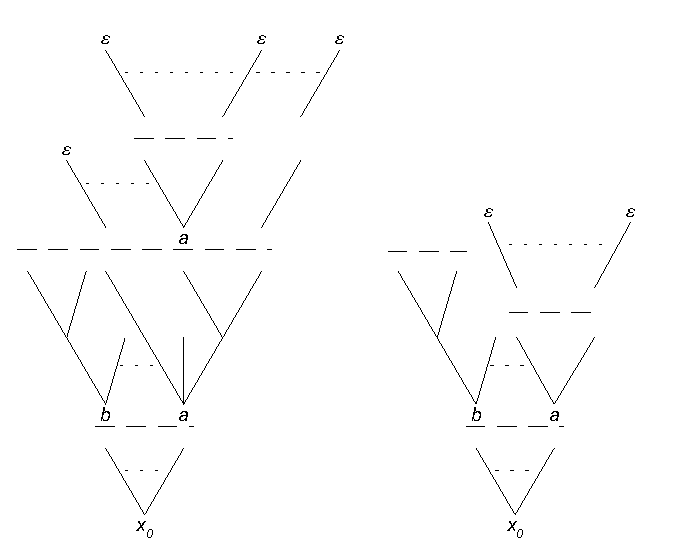
\includegraphics{img/stromy}
    \caption{Vytváranie redukovaného odvodenia} \label{strom}
    \end{figure}

    Označme $m$ dĺžku najdlhšej pravej strany spomedzi všetkých
    pravidiel $G'$ a $n=|V\union\{x_0\}|$. Tvrdíme, že stačí zvoliť:
    \[
    k=3m^n
    \]
    Pre $\forall w\neq\eps,w\in L(G')$ s odvodením $x_0\Ra
    w_0\Ra w_1\Ra\cdots\Ra w_n\equiv w$ bez újmy na všeobecnosti
    predpokladajme, že toto je redukované. Výskyt symbolu $a$ v jednom
    zo slov $w_i$ nazveme neproduktívny $\Longleftrightarrow$ ak tento
    výskyt je návestím koreňa podstromu, ktorého všetky listy majú
    návestie $\eps$. Inak výskyt nazveme produktívny. Pokiaľ
    $w\neq\eps$, tak $w_i$ obsahuje najmenej jeden produktívny
    symbol, navyše počet produktívnych symbolov vo $w_i\leq|w|$. Stačí
    nám ukázať, že $\forall i$, keď $Q$ je podslovo $w_i$ a platí
    $|Q|=3m^n$, potom $Q$ obsahuje najmenej jeden produktívny symbol.
    Pre $i<n$ žiadne podslovo $w_i$ nie je dlhšie ako $3m^n$. Pre
    $i=n+j,j\geq0$ predpokladajme, že $Q$ je podslovo $w_i,|Q|=3m^n$.
    $Q$ môžeme zapísať nasledovne:
    \[
    Q=Q_1Q_2Q_3,|Q_1|=|Q_2|=|Q_3|=m^n
    \]
    Predpokladajme, že $Q$ obsahuje iba neproduktívne symboly.
    Uvažujme nejaký výskyt symbolu $a$ v $Q_2$. Existuje jediný výskyt
    symbolu $b$ vo $w_{i-n}$ taký, že $a$ je návestie v strome $T$,
    ktorého koreň má návestie $b$. Ďalej, voľbou $Q,m,n$ všetky listy
    v $T$ majú návestia $\eps$. To je spor, lebo potom existuje
    v $T$ vetva s dvoma uzlami s rovnakým návestím
\end{dokaz}

\begin{veta}
    (O lineárnom priestore)
    \\ Nech $A$ je Turingov
    stroj\footnote{definície, popis modelu a iné v \cite{Hopc}} (TS)
    taký, že existuje $k$ také, že pre každé slovo $w$ tento TS
    použije pri práci na $w$ najviac $k|w|$ políčok. Potom
    $L(A)\in\mathcal{L}_{ECS}$
\end{veta}

\begin{veta}
    $\mathcal{L}_{OL}\subseteq\mathcal{L}_{ECS}$
\end{veta}

\begin{dokaz}
    Použijeme lemu \ref{linear} a na základe vety o lineárnom
    priestore, ktorá potom pre $OL$-jazyky platí, dostávame
    $L(G)\in\mathcal{L}_{ECS}$
\end{dokaz}

\subsection {Rozšírené $OL$-systémy ($EOL$-systémy)}

Ako sa pri $OL$-systémoch ukázalo, paralelné prepisovanie symbolov
nám istú silu pridalo, no fakt, že do jazyka sme museli zahrnúť
všetko, čo sme vyrobili (každú vetnú formu), nám veľkú časť nášho
optimizmu odobral. $EOL$-systémy nám dovolia opäť (ako pri
gramatikách Chomského hierarchie) filtrovať vetné formy rozdelením
množiny symbolov na terminály a neterminály. Do akej miery sa nám
tým náš model zosilní (malo by byť jasné, že jeho sila bude
minimálne taká, ako sila $OL$-systémov) si ukážeme na príklade
neskôr

\begin{definicia}
    $EOL$-systém je štvorica $G=(N,T,P,w), P\subseteq (N\union
    T)\times(N\union T)^{*}$ a $\forall a\in (N\union T)$ existuje v $P$
    pravidlo
\end{definicia}

\begin{definicia}
    Krok odvodenia je relácia $\Ra$ na $(N\union T)^{*}$ definovaná
    nasledovne: \mbox{$u\Ra v$} práve vtedy, keď $u=a_{1}\dots
    a_{n},\forall i\med a_{i}\in(N\union T),v=b_{1}\dots b_{n},\forall
    i\med b_{i}\in(N\union T)^{*}$ a $\forall i\med a_{i}\ra b_{i}\in P$
\end{definicia}

\begin{definicia}
    Jazyk generovaný $EOL$-systémom $G$ je $L(G)=\{x\in T^{*}\mm
    w\overset{*}\Ra x\}$
\end{definicia}

\begin{priklad}
    $G_{1}=(\{\sigma\},\{a,b\},\{\sigma\ra a,\sigma\ra b,a\ra
    a^{2},b\ra b^{2}\},\sigma)$, potom zjavne jazyk
    $L(G_{1})=\{a^{2^{n}}\mm n\geq0 \}\union\{b^{2^{n}}\mm
    n\geq0\}\not\in\mathcal{L}_{OL}$\\ Tento príklad ukazuje, že
    $EOL$-systémy sú silnejšie ako obyčajné $OL$-systémy a tým sme
    vlastne dali odpoveď na otázku, ktorú sme si položili na začiatku
    kapitoly, v tomto prípade sa sila neterminálu prejavila v tom, že
    nám umožnila spraviť zjednotenie dvoch jazykov
\end{priklad}

\begin{priklad}
    $G_{2}=(\{A\},\{a,b\},\{A\ra A,A\ra a,a\ra a^{2},b\ra b\},AbA)$
    potom jazyk ge\-ne\-ro\-va\-ný $G$ je
    $L(G_{2})=\{a^{2^{n}}ba^{2^{m}}\mm
    m,n\geq0\}\not\in\mathcal{L}_{OL}$
\end{priklad}

\begin{priklad}
    \label{efko}
    $G_{3}=(\{S,A,B,C,\bar{A},\bar{B},\bar{C},F\},\{a,b,c\},P,S)$
    \begin{tabbing}
    \= xxx \= $P=\{\med$ \= xxxxxxxxxx \= xxxxxxxxxx \= xxxxxxxxxx
    \= xxxxxxxxxx
    \kill
    \> \> $P=\{\med$ \> $S\ra ABC$ \> $a\ra F$ \> $b\ra F$ \> $c\ra
    F$\\
    \> \> \> $A\ra A\bar{A}$ \> $A\ra a$ \> $\bar{A}\ra\bar{A}$ \> $\bar{A}\ra
    a$\\
    \> \> \> $B\ra B\bar{B}$ \> $B\ra b$ \> $\bar{B}\ra\bar{B}$ \> $\bar{B}\ra
    b$\\
    \> \> \> $C\ra C\bar{C}$ \> $C\ra c$ \> $\bar{C}\ra\bar{C}$ \> $\bar{C}\ra
    c$\\
    \> \> \> $F\ra F\med\}$
    \end{tabbing}
    Možno niekoho prekvapí fakt, že $L(G_{3})=\{a^{n}b^{n}c^{n}\mm
    n\geq1\}$, no ak sa nad systémom $G_{3}$ trošku zamyslíme, tak sa
    nám táto skutočnosť ihneď vyjasní. Ide tu totiž o rafinované
    využitie neterminálu $F$ na to, aby terminálne slová vznikali
    naraz (teda slová z jazyka $L(G_{3})$ vznikajú v jednom kroku
    odvodenia prepísaním všetkých neterminálov na terminálne symboly).
    Ako si v nasledovnej vete ukážeme, tento jav nie je ani zďaleka
    taký zriedkavý, ako by sa mohlo zdať
\end{priklad}

\begin{veta}(Synchronizovaný tvar $EOL$-systému)
    \\ Nech $G=(N,T,P,w)$ je $EOL$-systém pre jazyk $L$. Potom existuje
    taký $EOL$-systém $G'$, $L(G')=L(G)$, že všetky jeho terminálne
    slová vznikajú z neterminálnych vetných foriem v jednom kroku
    odvodenia\footnote{teda keď sa vo vetnej forme objaví prvý
    terminál, tak nutnou podmienkou, aby sme niekedy vygenerovali
    terminálne slovo je, aby v kroku odvodenia, kedy sa do vetnej
    formy dostal, ``zterminálnela'' vetná forma celá}
\end{veta}

\begin{dokaz}
    Ukážeme konštrukciu synchronizovaného $EOL$-systému $G'$. Najskôr
    si vytvoríme nové neterminály, ktoré budeme potrebovať:
    \begin{itemize}
    \item $\forall a\in T$ vytvoríme $\xi_a$ (ak $a,b\in T$, tak
    $\xi_a\neq\xi_b$)
    \item $F,\sigma'$, budú predstavovať FALSE, resp. nový počiatočný
    symbol
    \end{itemize}
    Označme $N'=\{\xi_a\mm a\in T\}$. Pre jednoduchosť zaveďme
    niekoľko pojmov, ktoré neskôr využijeme:
    \begin{enumerate}
    \item Nech $S$ je ľubovoľná množina reťazcov z $(N\union T)^*$, pre
    ňu definujeme množinu $A(S)$ nasledovne:
    \begin{enumerate}
    \item reťazec $b_{1}\dots b_{n}\in A(S)\overset{def}
    \Longleftrightarrow$ ak existuje reťazec $a_{1}\dots a_{n}\in S$
    taký, že buď $b_i=a_i$ alebo $a_i\in T$ a $b_i=\xi_i$ (teda
    $b_i\in N'$), potom $A(S)\subset(N\union N'\union T)^*$
    \item ak $S\neq\emptyset$, potom $A(S)\neq\emptyset$, lebo
    $S\subseteq A(S)$
    \end{enumerate}
    \item $\delta_P(a)$ nazveme množinu všetkých pravých strán
    pravidiel pre symbol $a$ z $P$
    \end{enumerate}
    Definujme synchronizovaný $EOL$-systém $G'$ nasledovne: $G'=(N\union
    N'\union\{F,\sigma'\},T,P',\sigma')$, pričom
    \begin{tabbing}
    \= xxx \= $P'\med$: \= xxxxxxxxxxxxxxxx \= xxxxxxxxxxx \kill \>\>
    $P':$ \> $\delta_{P'}(\sigma')=A(\{w\})$\\ \>\>\> $\forall
    a\in(T\union \{F\})$ \> $(a\ra F)\in P'$\\ \>\>\> $\forall a\in N$
    \> $\delta_{P'}(a)=A(\delta_P(a))$\\ \>\>\> $\forall\xi_a\in N'$
    \> $\delta_{P'}(\xi_a)=A(\delta_P(a))$
    \end{tabbing}
    Malo by byť zrejmé, že teminálne slová musia v $G'$ vznikať naraz,
    pretože ak sa náhodou nejaký terminál do venej formy dostane skôr
    ako ostatné, tak sa v ďaľšom kroku prepíše nutne na $F$ a z $F$ sa
    už nikdy terminál nestane. Rovnako zrejmé by malo byť
    $L(G')=L(G)$, pretože nové neterminály $\xi_i$ vo vetnej forme
    akoby nahrádzali terminálne symboly, a tak simulovali odvodenie v
    pôvodnom systéme $G$
\end{dokaz}

\begin{veta}
    Každý konečný jazyk je v $\mathcal{L}_{EOL}$
\end{veta}

\begin{dokaz}
    Nech $L$ je konečný, potom existuje regulárna gramatika $G$ taká,
    že $L=L(G)$. Táto regulárna gramatika je ale zároveň (po doplnení
    pravidiel $a\ra a\med\forall a\in(N\union T)$) aj hľa\-da\-ným
    $EOL$-systémom
\end{dokaz}

\begin{lema}
    \label{norm_tvarEOL} Nech $G$ je $EOL$-systém, potom existuje
    $EOL$-systém $G'$, ktorého všetky pravidlá obsahujúce $a\in T$ na
    ľavej strane sú tvaru $a\ra a$
\end{lema}

\begin{dokaz}
    Zkonštruujeme $EOL$-systém $G'$ nasledovne: pre každé $a\in T$
    zavedieme nový neterminál $\xi_{a}$ a upravíme pravidlá:
    \begin{enumerate}
    \item tie pravidlá, kde sa vyskytujú terminály, nahradíme novými tak,
    že všetky terminály (na ľavej i pravej strane) zmeníme na
    príslušné nové neterminály ($a\in T$ nahradíme $\xi_{a}\in N$)
    \item pre každé $a\in T$ pridáme pravidlo $a\ra a$
    \item pre každé nové $\xi_{a}\in N$ pridáme pravidlo $\xi_{a}\ra a$
    \end{enumerate}
\end{dokaz}

\begin{veta}
    Trieda $\mathcal{L}_{EOL}$ je uzavretá na
    $\union,\cdot,+,\intersect\mathcal{R},h_{\eps}$ a nie je uzavretá
    na $h^{-1}$
\end{veta}

\begin{dokaz}
    Dokážeme iba dve vlastnosti, väčšina ostatných dôkazov sa až na
    malé technické detaily veľmi nelíši od známych konštrukcií pre
    bezkontextové gramatiky:
    \begin{itemize}
    \item $\union :$ Máme $EOL$-systémy $G_{1}$ pre $L_{1}$ a $G_{2}$
    pre $L_{2}$. Ku $G_{1},G_{2}$ spravíme normálne tvary
    $G'_{1},G'_{2}$ podľa konštrukcie z lemy \ref{norm_tvarEOL}. Bez
    ujmy na všeobecnosti môžeme predpokladať, že $N'_{1}\intersect
    N'_{2}=\emptyset$. Vytvoríme $G_{3}$ pre $L_{1}\union L_{2}$
    nasledovne: zavedieme nový neterminál $\sigma_{3}$ tak, že
    $\sigma_{3}\not\in N'_{1}$ \mbox{a $\sigma_{3}\not\in N'_{2}$}.
    Ďalej $N_{3}=N'_{1}\union N'_{2}\union\{\sigma_{3}\}$,
    $T_{3}=T'_{1}\union T'_{2}$, $P_{3}=P'_{1}\union
    P'_{2}\union\{\sigma_{3}\ra\sigma'_{1}|\sigma'_{2}\}$ \mbox{a
    nakoniec} $G_{3}=(N_{3},T_{3},P_{3},\sigma_{3})$
    \item $h^{-1} :$ Zoberme jazyk $L\in\mathcal{L}_{EOL},
    L=\{a^{2^n}\mm n\geq0\}$ a definujme homomorfizmus $h$ nasledovne:
    $h(a)=a, h(b)=\eps$. Potom $h^{-1}(L)=\{w\in\{a,b\}^*\mm
    \#_a w=2^n,n\geq0\}$. Ukážeme, že
    $h^{-1}(L)\not\in\mathcal{L}_{EOL}$. Nech $G$ je $EOL$-systém pre
    $h^{-1}(L)$. Zoberme $w_0\in h^{-1}(L)$, nech $\#_a w_0=n$.
    Zoberme ľubovoľné dve $a$, medzi ktorými sú iba $b$. Ak je medzi
    týmito dvoma $a$ ``príliš veľa''\footnote{tento počet vieme určiť,
    závisí napr. od dĺžky najdlhšej pravej strany pravidla v $G$,
    bližšie v \cite{clos}} $b$, tak takéto slovo nedokážeme vyrobiť
    (nemáme na to dostatok času), čo je spor s tým, že $G$ je
    $EOL$-systém pre $h^{-1}(L)$
    \end{itemize}
\end{dokaz}

\begin{veta}
    $\mathcal{L}_{CF}\subsetneq\mathcal{L}_{EOL}$
\end{veta}

\begin{dokaz}
    Každá bezkontextová gramatika vyhovuje definícii $EOL$-systému (po
    doplnení pravidiel $a\ra a\med\forall a\in(N\union T)$), teda platí
    nevlastná inklúzia $\mathcal{L}_{CF}\subseteq\mathcal{L}_{EOL}$.
    Že platí aj vlastná inklúzia, sme ukázali v príklade \ref{efko},
    kde sme našli $EOL$-systém pre jazyk $L=\{a^{n}b^{n}c^{n}\mm
    n\geq1\}\in\mathcal{L}_{CS} - \mathcal{L}_{CF}$
\end{dokaz}

\begin{poznamka}
    $1L$ a $2L$-systémy sú nejakou analógiou kontextových gramatík, i
    keď o ich sile by sa dali viesť podobné diskusie ako pri
    $OL$-systémoch. Snáď len toľko, že obojstranný kontext je silnejší
    ako jednostranný a oba systémy sú silnejšie ako $OL$-systémy
\end{poznamka}

\subsection{$TOL$-systémy (table)}

Tieto systémy nebudeme striktne definovať, povieme si len základné
veci, ktorými sa od kla\-sic\-kých $OL$-systémov odlišujú.
$TOL$-systém $G=(V,P_{1},\dots,P_{k},w_{0})$ má niekoľko
(konkrétne $k$) sád pravidiel, v danom kroku odvodenia použijeme
na vetnú formu iba jednu sadu pravidiel

\begin{priklad}
    $G=(\{a\},\{a\ra a^{2}\},\{a\ra a^{3}\},a)$, potom
    $L(G)=\{a^{2^{n}}a^{3^{m}}\mm n,m\geq0\}\not\in\mathcal{L}_{OL}$
\end{priklad}

\begin{poznamka}
    Trieda $\mathcal{L}_{TOL}$ zdieľa ``zlé'' uzáverové vlastnosti
    triedy $\mathcal{L}_{OL}$. Podobne ako pre $\mathcal{L}_{OL}$
    platí aj pre $\mathcal{L}_{TOL}$ vzťah
    $\mathcal{L}_{TOL}\subseteq\mathcal{L}_{ECS}$
\end{poznamka}

\section{Ďaľšie paralelné gramatiky}

\subsection{Indické paralelné gramatiky}

\begin{definicia}
    Indická paralelná gramatika (IP) je štvorica $G=(N,T,P,\sigma)$,
    pričom \mbox{$\sigma\in N$} $N\intersect T=\emptyset, P\subseteq
    N\times(N\union T)^{*}$
\end{definicia}

\begin{definicia}
    Krok odvodenia IP $G$ je relácia $\Ra$ keď sa všetky výskyty
    zvoleného neterminálu prepíšu naraz tým istým pravidlom
\end{definicia}

\begin{priklad}
    $G_{1}=(\{\sigma\},\{a\},\{\sigma\ra\sigma\sigma,\sigma\ra
    a\},\sigma)$ potom $L(G_{1})=\{a^{2^{n}}\mm n\geq0\}$
\end{priklad}

\begin{priklad}
    Dyckov jazyk nad dvoma písmenkami $D_{1}$ (jazyk správne
    uzátvorkovaných výrazov) nie je $\mathcal{L}_{IP}$
\end{priklad}

\begin{dokaz}
    Sporom predpokladajme, že $D_{1}\in\mathcal{L}_{IP}$, potom
    existuje IP gramatika $G$ taká, že \mbox{$L(G)=D_{1}$}. Ukážeme,
    že by musela mať nekonečne veľa neterminálov, čo nie je možné. Pre
    jednoduchosť označme $L=D_{1}$. Vytvoríme v $L$ hierarchiu tvarov
    slov nasledovne: definujme rekurentne podmnožiny $L$ a uvedomme
    si, koľko najmenej neterminálov treba na generovanie slov z každej
    z nich:
    \begin{description}
    \item{$\med$} $L_{1}=\{\med a^{n}b^{n}\mm n\geq1\med\}^{+}$ treba aspoň 2
    neterminály
    \item{$\med$} $L_{i+1}=\{\med a^{n}wb^{n}\mm w\in L_{i},n\geq1\med\}^{+}$
    treba aspoň $i+2$ neterminálov
    \end{description}
    Ako vidno, táto hierarchia je nekonečná, teda na generovanie
    $(\bigcup_{i=1}^{\infty}L_{i})\subseteq L$ je treba nekonečne veľa
    neterminálov
\end{dokaz}

\begin{veta}
    $\mathcal{L}_{IP}\intersect\mathcal{L}_{CF}=\mathcal{L}_{DBL}$
\end{veta}

\begin{poznamka}
    $\mathcal{L}_{DBL}$ je trieda {\it Derivation Bounded Languages},
    ku každému jazyku z tejto triedy existuje $k$ také, že počet
    neterminálov v každej vetnej forme je menší ako $k$
\end{poznamka}

\begin{veta}
    $\mathcal{L}_{IP}\subseteq\mathcal{L}_{ECS}$
\end{veta}

\begin{veta}
    $\mathcal{L}_{IP}$ je uzavretá na $\union,\cdot,*,h$
\end{veta}

\begin{veta}
    $\mathcal{L}_{IP}$ je neporovnateľná s $\mathcal{L}_{EOL}$
\end{veta}

\begin{veta}
    $\mathcal{L}_{IP}\subseteq\mathcal{L}_{ETOL}$ (extended $TOL$)
\end{veta}

\subsection{Ruské paralelné gramatiky}

\begin{definicia}
    Ruská paralelná gramatika je pätica $G=(N,T,P_{1},P_{2},\sigma)$,
    pričom $\sigma\in N$, \mbox{$N\intersect T=\emptyset$}, $P_{1}, P_{2}$
    sú konečné množiny pravidiel, $P_{1},P_{2}\subseteq N\times(N\union
    T)^{*}$
\end{definicia}

\begin{definicia}
    Krok odvodenia: všetky výskyty zvoleného neterminálu sa prepíšu
    naraz istým pravidlom z $P_{1}$, alebo sa prepíše práve jeden
    neterminál pravidlom z množiny $P_{2}$
\end{definicia}

\subsection{Absolútne paralelné gramatiky}

\begin{definicia}
    Absolútne paralelná gramatika (AP) je štvorica $G=(N,T,P,\sigma)$,
    kde \mbox{$\sigma\in N$}, $N\intersect T=\emptyset$, $P$ je konečná
    množina pravidiel tvaru
    $(A_{1},\dots,A_{n})\ra(w_{1},\dots,w_{n})$, kde \mbox{$\forall
    A_{i}\in N$}, $w_{i}\in(N\union T)^{*}$
\end{definicia}

\begin{definicia}
    Krok odvodenia je relácia $w\Ra v$ práve vtedy, keď
    $w=u_{1}A_{1}u_{2}A_{2}\dots u_{n}A_{n}u_{n+1}$ \mbox{a
    $v=u_{1}w_{1}u_{2}w_{2}\dots u_{n}w_{n}u_{n+1}$}, pričom
    $u_{1},\dots u_{n+1}\in T^{*}$ (t.j. naraz prepisujeme všetky
    neterminály vo vetnej forme, na každú možnosť výskytu neterminálov
    musíme mať pravidlo)
\end{definicia}

\begin{priklad}
    Pozrime sa na AP gramatiku:\\
    $G=(\{S\},\{a,b,c\},\{(S)\ra(SSS),(S,S,S)\ra (aS,bS,cS),(S,S,S)\ra
    (a,b,c)\},S)$ potom $L(G)=\{a^{n}b^{n}c^{n}\mm n\geq1\}$
\end{priklad}

\begin{veta}
    $\mathcal{L}_{AP}$ je $\mathcal{AFL}$
\end{veta}

\begin{veta}
    $\mathcal{L}_{AP}\intersect 2^{a^{*}}\subseteq\mathcal{R}$ (t.j.
    jednopísmenkové $AP$ jazyky sú regulárne)
\end{veta}

\begin{dokaz}
    Nech $L\in\mathcal{L}_{AP}$ a $G=(N,T,P,A_p)$ je $AP$ gramatika
    taká, že $L(G)=L$. Bez újmy na všeobecnosti môžeme predpokladať,
    že $T=\{a\}$. Nech \mbox{$N=\{A_1,\dots,A_n\}$}. Definujme $N'$
    nasledovne: $N'=\{A_p\}\union\{A_{i_1,\dots,i_k}\mm\forall j\med
    A_{i_j}\in N,\med A_{i_1},\dots,A_{i_k}$ sa nachádzajú na pravej
    strane niektorého (rovnakého) z pravidiel $P$ v tomto poradí$\}$.
    Bez újmy na všeobecnosti môžeme pred\-pokla\-dať, že všetky
    pravidlá z $P$ sú tvaru
    $(A_{i_1},\dots,A_{i_m})\ra(a^{k_1}\pi_1,\dots,a^{k_m}\pi_m)$, kde
    $\forall i\med \pi_i\in N^*$. Definujme
    $\varphi_i=i_1,\dots,i_l\Longleftrightarrow\pi_i=A_{i_1}\dots
    A_{i_l}$ Vytvoríme množinu pravidiel $P'$ nasledovne:
    \[
    A_{i_1,\dots,i_k}\ra
    a^{w_1+\cdots+w_k}A_{\varphi_{i_1},\dots,\varphi_{i_k}}\in
    P'\Longleftrightarrow
    (A_{i_1},\dots,A_{i_k})\ra(a^{w_1}\pi_1,\dots,a^{w_k}\pi_k)\in P
    \]
    Teraz definujme $G'=(N',\{a\},P',A_p)$. $G'$ je zrejme regulárna
    gramatika a z konštrukcie vyplýva, že $L(G')=L(G)$
\end{dokaz}

\begin{veta}
    $\mathcal{L}_{AP}=\mathcal{L}_{2DAP}$
\end{veta}

\begin{poznamka}
    $\mathcal{L}_{2DAP}$ je trieda jazykov, ktoré sú generované
    dvojsmernými determi\-nis\-tic\-ký\-mi $a$-prek\-la\-dač\-mi
\end{poznamka}

\chapter{Generatívne systémy}

Doteraz sme sa zaoberali iba paralelnými modelmi, ktorých
spoločnou črtou bola akási\linebreak ``gramatiková filozofia'',
teda mali sme množinu symbolov, počiatočný symbol, resp.
počiatočné slovo a akúsi množinu prepisovacích pravidiel, ktoré
striktne riadili odvodenie a celý mechanizmus generoval nejaký
jazyk. Ukážeme si trošku iný pohľad na vec, nový z hľadiska
spôsobu prepisovania, kedy zostane zachovaná ``viditeľná
gramatiková časť'', teda symboly, počiatočný symbol, zmení sa však
prepisovací mechanizmus. Ako uvidíme neskôr, pôjde o akúsi
kombináciu gramatikového a automatového pohľadu na jazyky. Pomocou
tohto mechanizmu bude možné simulovať už známe gramatiky, či už z
Chomského hierarchie, alebo skôr spomenuté paralelné gramatiky.
Zaujímavý (a veľmi dôležitý) na tomto modeli je fakt, že pomerne
jednoducho umožní porovnať paralelné a sekvenčné formalizmy z
hľadiska zložitosti, a tým ukázať, v ktorej oblasti nám
paralelizmus pomôže a kde naopak nemá zmysel sa ním veľmi
zaoberať.

\section{Definície a označenia}

\begin{definicia}
Abstraktný generatívny systém je štvorica $G=(N,T,f,\sigma)$ kde
$N$ je množina neterminálov, $T$ je množina terminálov, $f$ je
konečne zadaná funkcia $(N\cup T)^* \ra 2^{(N\cup T)^* }$,
$\sigma$ je počiatočný neterminál pričom $N,T$ nie sú nutne
disjunktné abecedy.
\end{definicia}

\begin{definicia}
Krok odvodenia abstraktného generatívneho sytému je relácia $\Ra$
na $(N\cup T)^* $ definovaná takto: $u\Ra v$ práve vtedy keď $v\in
f(u)$.
\end{definicia}

\begin{definicia}
Jazyk generovaný abstraktným generatívnym systémom $G$ je množina
$L(G)$, pričom \mbox{$L(G)=\{w\in T^* \mm\sigma\overset{* }\Ra
w\}$}.
\end{definicia}

V ďalšom sa budeme zaoberať špeciálnym typom abstraktných
generatívnych systémov, a to generatívnymi systémami.

\begin{definicia}
1-$a$-prekladač je $a$-prekladač
$M=(K,\Sigma_1,\Sigma_2,H,q_0,F)$, v ktorom množina štvoríc je
tvaru\footnote{1-$a$-prekladač nemá pružnú čítaciu hlavu t.j. môže
čítať práve jeden symbol} $H\subseteq K\times\Sigma_1\times
{\Sigma_2}^* \times K$.
\end{definicia}

\begin{definicia}
Generatívny systém ($g$-systém) je abstraktný generatívny systém,
v ktorom $f$ je zobrazenie 1-$a$-prekladačom. Zapisujeme
$G=(N,T,M,\sigma)$ kde $M$ je 1-$a$-prekladač.
\end{definicia}

\begin{definicia}
Krok odvodenia $g$-systému je relácia $\Ra$ na $(N\cup T)^* $
definovaná takto: $u\Ra v$ práve vtedy\footnote{pre vstupné slovo
$u$ 1-$a$-prekladač $M$ vygeneruje výstup $v$} keď $v\in M(u)$.
\end{definicia}

\begin{priklad}
\label{gs_prikl_aprekladac} Zostrojíme $g$-systém  $G=(N,T,M,S)$ pre jazyk
$L=\{ww\mm w\in\{a,b\}^*\}$. Neterminály budú $N=\{S,A\}$,
terminály $T=\{a,b\}$, $a$-prekladač $M$ bude (obr.\ref{fig:gsystem-priklad}).
\begin{figure}[!ht]
  \centering
  \includegraphics{img/gsystems/gsystem-priklad.1.mps}
  \caption{$a$-prekladač $g$-systému pre jazyk $L$ z príkladu
    \ref{gs_prikl_aprekladac}}
  \label{fig:gsystem-priklad}
\end{figure}
\end{priklad}

\begin{oznacenie}
$\mathcal{G}$  trieda všetkých $g$-systémov. \\
$\mathcal{G_\varepsilon}$ trieda všetkých bez-$\varepsilon$
$g$-systémov, t.j. 1-$a$-prekladač nedáva na výstup $\varepsilon$.
\end{oznacenie}

\section{Porovnanie generatívnej sily $g$-systémov s gramatikami Chomského hierarchie}

\begin{veta}
\label{gs_veta_gre} $\mathcal{L}_{\mathcal{G}}=\mathcal{L}_{RE}$
\end{veta}

\begin{dokaz}
Dokážeme obe inklúzie:
\begin{description}
\item{$\subseteq$:} Táto inklúzia vyplýva z Turingovej tézy, ale
iste by sme si vedeli predsaviť aj TS, ktorý dostane na pásku
slovo a na druhej páske simuluje odvodenie tohto slova
$g$-systémom od počiatočného neterminálu a porovnáva, či je slovo
z druhej pásky zhodné so vstupom na prvej páske.
\item{$\supseteq$:} Pomocou $g$-systémov chceme simulovať frázové gramatiky, t.j. ku každej
frázovej gramatike $G$ treba zostrojiť $g$-systém $G'$ taký, že
$L(G')=L(G)$. $G'$ zostrojíme nasledovne:\newline ku každému
pravidlu $a_1a_2\dots a_n\ra b_1b_2\dots b_m$ urobíme v
$g$-systéme cestu ako na\linebreak obrázku \ref{fig:re-to-gsystem}.
\end{description}
\end{dokaz}

\begin{figure}[!ht]
    \centering
    \includegraphics{img/gsystems/re-to-gsystem.1.mps}
    \caption{Konštrukcia $g$-systému ku frázovej gramatike}
    \label{fig:re-to-gsystem}
\end{figure}

\pagebreak

\begin{veta}
\label{gs_veta_gre2}
$\mathcal{L}_{\mathcal{G}_\varepsilon}=\mathcal{L}_{CS}$
\end{veta}

\begin{dokaz}
Dokážeme obe inklúzie:
\begin{description}
\item{$\subseteq$:} K bez-$\varepsilon$ $g$-systému zostrojíme LBA
akceptujúci ten istý jazyk. LBA si, rovnako ako TS\linebreak v
predchádzajúcej vete, vyrobí druhú pásku, na ktorej bude simulovať
odvodenie vstupného slova simulovaným $g$-systémom. Keďže
$g$-systém je bez $\varepsilon$, nemôže sa stať, že pri odvodení
nejakého slova $w$ vznikne vetná forma dĺžky väčšej ako je $|w|$.
Preto na simuláciu stačí priestor ohraničený dĺžkou vstupného
slova, a teda vystačíme s LBA.
\item{$\supseteq$:} Konštrukcia je podobná ako v predchádzajúcej vete
(obr.\ref{fig:cs-to-gsystem}) s využitím toho, že v kontextových gramatikách nie
je pravá strana pravidla kratšia ako ľavá, takže v konštrukcii
1-$a$-prekladača nepotrebujeme pravidlá s $\varepsilon$ výstupom.
\end{description}
\end{dokaz}

\begin{figure}
    \centering
    \includegraphics{img/gsystems/cs-to-gsystem.1.mps}
    \caption{Konštrukcia $g$-systému ku kontextovej gramatike}
    \label{fig:cs-to-gsystem}
\end{figure}

\begin{definicia}
Kopírovací cyklus v 1-$a$-prekladači je štvorica z $H$ tvaru
$(q,a,a,q)$.
\end{definicia}

\begin{definicia}
$g$-systém je sekvenčný, ak jediné cykly v 1-$a$-prekladači sú
kopírovacie cykly v počiatočnom alebo koncovom stave.
\end{definicia}

\begin{oznacenie}
$\mathcal{S}$ trieda všetkých sekvenčných $g$-systémov.\\
$\mathcal{S}_\varepsilon$ trieda všetkých bez-$\varepsilon$
sekvenčných $g$-systémov.
\end{oznacenie}

\pagebreak

\begin{veta}\label{gs_veta_gsek}
$\mathcal{L}_{\mathcal{S}}=\mathcal{L}_{RE},
\mathcal{L}_{\mathcal{S}_\varepsilon}=\mathcal{L}_{CS}$
\end{veta}

\begin{dokaz}
Konštrukcia je tá istá ako vo vete \ref{gs_veta_gre}, resp.
\ref{gs_veta_gre2}, lebo ľahko vidno, že zostrojený $g$-systém je
sekvenčný.
\end{dokaz}

\section{Modelovanie známych gramatík pomocou $g$-systémov}

\begin{priklad}
    Ukážeme si, že pomocou $g$-systémov vieme jednoducho modelovať
    $EOL$ a bezkontextové gramatiky:
    \begin{description}
    \item{$EOL$:} Nech množina pravidiel $EOL$ je
        $P=\{ a_1\pravidlo u_1,a_2\pravidlo u_2,\dots,a_n\pravidlo
        u_n\}$.
        Potom príslušný $g$-systém bude vyzerať ako na obrázku
        \ref{fig:eol-to-gsystem}a.

    \item{$CF$:} Nech množina pravidiel $CF$ je
        $P=\{a_1\pravidlo u_1, a_2\pravidlo u_2,\dots,a_n\pravidlo
        u_n\}$. Príslušný $g$-systém zostrojíme podľa obrázku
        \ref{fig:eol-to-gsystem}b.
    \end{description}

    \begin{figure}[!ht]
        \centering
        \subfigure[EOL]{
            \includegraphics{img/gsystems/eol-to-gsystem.1.mps}
        }
        \subfigure[CF]{
            \includegraphics{img/gsystems/cf-to-gsystem.1.mps}
        }
        \caption{Modelovanie $EOL$-systémov a
                    $CF$-gramatík pomocou $g$-systémov}
        \label{fig:eol-to-gsystem}
    \end{figure}
\end{priklad}

\begin{poznamka}
Gramatika $G$ je bezkontextová práve vtedy, keď existuje sekvenčný
$g$-systém $G'$ s dvoma stavmi taký, že $L(G)=L(G')$. Implikácia
``$\Ra$'' vyplýva z konštrukcie na\linebreak obrázku \ref{fig:eol-to-gsystem}b,
dôkaz opačnej implikácie nie je triviálny a presahuje rámec tohto
textu.
\end{poznamka}

\begin{veta}
Absolutne paralelné gramatiky sú ekvivalentné s $g$-systémami
spĺňajúce nasledujúce podmienky (ozn. $\tilde{\mathcal{G}}$ trieda
takýchto $g$-systémov):
\begin{enumerate}
  \item každý cyklus je kopírovací cyklus pre terminál
  \item v každom stave je kopírovací cyklus pre každé $a\in T$
  \item terminálne symboly sú prepisované len v kopírovacích cykloch
\end{enumerate}
\end{veta}

\begin{dokaz}
Máme dokázať, že
$\mathcal{L}_{AP}=\mathcal{L}_{\tilde{\mathcal{G}}}$
\begin{description}
\item{$\subseteq$:} K danej $AP$ gramatike $G$ zkonštruujeme ekvivalentný $g$-systém
$G'\in\tilde{\mathcal{G}}$ nasledovne. Každému pravidlu v $G$
tvaru $(A_1,\dots A_k)\ra (w_1,\dots w_k))$ zodpovedá v
1-$a$-prekladači $g$-systému $G'$ práve jedna cesta znázornená na
obrázku \ref{fig:ap-to-gsystem}.

\begin{figure}[!ht]
    \centering
    \includegraphics{img/gsystems/ap-to-gsystem.1.mps}
    \caption{Konštrukcia $g$-systému k $AP$ gramatike}
    \label{fig:ap-to-gsystem}
\end{figure}

\item{$\supseteq$:} Pre každú cestu v 1-$a$-prekladači z $q_0$ do $q_F$
(mimo kopírovacích cyklov) v $AP$ gramatike urobíme pravidlo:
$(A_1,\dots A_k)\ra (w_1,\dots w_k))$.
\end{description}
\end{dokaz}

\section{Miery zložitosti}

\begin{itemize}
\item $STATE(G)=$ počet stavov 1-$a$-prekladača $g$-systému $G$
\item $ARC(G)=$ počet pravidiel 1-$a$-prekladača $g$-systému $G$
\item $STATE_U(L)=\min\{ STATE(G)\mm L=L(G), G\in U\}$
\item $ARC_U(L)=\min\{ ARC(G)\mm L=L(G), G\in U\}$
\item $TIME(G,w)=\min\{ k\mm\sigma\overset{k}{\underset{G}{\Ra}} w\}; w\in L(G)$
\item $TIME(G,n)=\max\{ TIME(G,w)\mm w\in L(G), |w|\leq n\}$
\item $TIME_U(f(n))=\{ L \mm \exists G\in U, L=L(G), TIME(G,n)=O(f(n))\}$
\item $\overline{TIME}_U(f(n))=\{ L\mm\forall G\in U, L=L(G), TIME(G,n)=\Omega(f(n))\}$
\item $SPACE(G,w)=\min\{ SPACE(\alpha )\}$; kde $\alpha$ : $\sigma\Ra u_1\Ra\dots\Ra u_n$ je odvodenie $w$ v $G$
a $SPACE(\alpha)=\max\{|u_i|\mm 0\leq i\leq n\}$
\end{itemize}

\begin{veta}
Pre každý nekonečný jazyk $L$ platí:
\begin{enumerate}
\item $L\in\overline{TIME}_{\mathcal{S}}(n)$
\item $L\in\overline{TIME}_{\mathcal{G}}(\log n)$
\end{enumerate}
\end{veta}

\begin{dokaz}
\begin{enumerate}
\item Nech $G\in\mathcal{S}$. Zamyslime sa nad tým, aké najdlhšie
slovo môže vygenerovať $G$ na $n$ krokov. $G$ dokáže v jednom
kroku prepisovať len jeden súvislý úsek vetnej formy. Túto vetnú
formu dokáže $G$ predĺžiť o najviac

\centerline{$m=\max\{$ súčet dĺžok výstupov na jednej ceste v
1-$a$-prekladači - dĺžka tejto cesty $\}$} Majme odvodenie $\sigma
=w_0\Ra w_1\Ra\dots\Ra w_i\Ra w_{i+1}\Ra\dots\Ra w_n$. Potom
platí\linebreak $|w_{i+1}|\leq |w_i| + m$. Keďže $|w_0|=|\sigma
|=1$, tak $|w_n|\leq 1 + nm$. Z toho teda nakoniec plynie, že $G$
potrebuje na vygenerovanie slova dĺžky $n$ aspoň lineárny čas.
\item Nech $G\in\mathcal{G}$. $G$ môže v každej vetnej forme
prepísať všetky symboly. Označme

\centerline{$m=\max\{$ výstup v 1-$a$-prekladači $\}$} Potom platí
$|w_{i+1}|\leq |w_i|.m$. Keďže $|w_0|=|\sigma |=1$, tak $|w_n|\leq
m^n$. Z toho plynie, že $G$ potrebuje na vygenerovanie slova dĺžky
$n$ aspoň logaritmický čas
\end{enumerate}
\end{dokaz}

\section{Porovnanie sekvenčných a paralelných $g$-systémov}
\label{gs_sec_sekvspar}

\begin{veta}
\label{gs_veta_parsek}
$\mathcal{L_G=L_S,L_{G_{\varepsilon}}=L_{S_{\varepsilon}}}$
\end{veta}

\begin{dokaz}
Tvrdenie priamo vyplýva z viet \ref{gs_veta_gre}, \ref{gs_veta_gre2} a
\ref{gs_veta_gsek} a hovorí nám, že paralelné a sekvenčné $g$-systémy
sú z hľadiska generatívnej sily ekvivalentné, no nedáva nám žiadny
návod, ako ku paralelnému $g$-systému nájsť sekvenčný, rovnako nič
nehovorí o tom, aký vplyv bude mať táto konštrukcia na popisnú
zložitosť.

Ukážeme si, ako k ľubovoľnému $g$-systému $G\in\mathcal{G}$
zkonštruujeme $g$-systém $G''\in\mathcal{S}$ \mbox{s ním}
ekvivalentný (t.j. $L(G)=L(G'')$) a potom si povieme, ako sa
``zosekvenčnenie'' odrazí na zložitosti.

Nech $G=(N,T,M,\sigma)$ je ľubovoľný $g$-systém,
$L(G)\in\mathcal{L_G}$, počiatočný stav $M$ je $q_0$ a koncový
$q_F$. Uvedomme si, čo potrebujeme na $G$ prepracovať, aby sme ho
``zosekvenčnili''. \mbox{V prvom} rade potrebujeme mať v
po\-čia\-toč\-nom aj koncovom stave kopírovacie cykly pre
všetky\footnote{ako sa neskôr ukáže, tak nie nutne pre úplne
všetky, stačí pre niektoré} symboly, aby sme sa vo vetnej forme
mohli presunúť ľubovoľne ďaleko, potom niečo $a$-prek\-la\-da\-čom
prepísať a vetnú formu dokopírovať do konca. V druhom rade
potrebujeme odstrániť \mbox{z $G$} vnútorné cykly (teda všetky
také, ktoré nie sú kopírovacími cyklami v počiatočnom,
\mbox{resp.} koncovom stave). Keď sa nám toto podarí, budeme s
konštrukciou hotoví. $G''$ budeme konštruovať v dvoch krokoch:
\begin{enumerate}
  \item Zostrojíme $G'=(N',T,M',\underline{\overline{\sigma}})$
  ekvivalentný s $G$ s užitočnými technickými vlastnosťami, ktoré
  neskôr využijeme:
  \begin{enumerate}
    \item zavedieme nový počiatočný stav $q_0'$ a nový koncový stav
    $q_F'$ a v týchto stavoch zkonštruujeme kopírovacie
    cykly\footnote{Zrejme by nestačilo dodať kopírovacie cykly do
    $q_0$, resp. $q_F$. Mohlo by sa totiž ľahko stať, že by sme takto
    zkonštruovaným 1-$a$-prekladačom akceptovali aj to, čo
    1-$a$-prekladač v $G$ neakceptoval} $\forall a\in(N'\cup T)$, $N'$
    definujeme neskôr, označme množinu týchto kopírovacích cyklov
    $C=\{(q,a,a,q)\mm q\in\{q'_0,q'_F\},a\in(N\cup T)\}$.
    \item $G'$ bude udržovať informáciu o prvom  a poslednom symbole
    vetnej formy tak, že ich označí: prvý symbol horným prúžkom,
    posledný dolným prúžkom. Označené symboly budú nové neterminály, v
    $G'$ musíme vytvoriť nové podčiarknuté aj nadčiarknuté symboly,
    teda $N'=N\cup\{\overline{a}\mm a\in(N\cup T
    )\}\cup\{\underline{a}\mm a\in(N\cup
    T)\}\cup\{\underline{\overline{\sigma}}\}$. Počiatočný neterminál
    $G'$ bude $\underline{\overline{\sigma}}$. Vetná forma bude
    vyzerať nasledovne: $\overline{a}_1 a_2 a_3\dots
    a_{n-1}\underline{a_n}$.
  \end{enumerate}
  Teraz poďme konštruovať $G'$ tak, aby sme zabezpečili obe
  ``dobré'' vlastnosti, ktoré sme uviedli a zároveň aby boli $G$ a
  $G'$ ekvivalentné. Zrejme bude potrebné upraviť prechodovú množinu
  1-$a$-prekladača. Ak $H$ bola prechodová množina $M$, tak $H_{M'}$
  bude prechodová množina $M'$. Zatiaľ definujme $H'$ nasledovne
  (nech $a,d,A,B\in(N\cup T),b,c\in(N\cup T)^*$):
  \[
  H'=H\cup C\cup\{(q'_0,\overline{A},\overline{a}b,q_1)\mm
  (q_0,A,ab,q_1)\in H\}\cup \{(q,\underline{B},c
  \underline{d},q'_F)\mm(q,B,cd,q_F)\in H\}
  \]
  Ak sa nad $H'$ trochu zamyslíme, tak je jasné, že v $q'_0$, resp.
  v $q'_F$ síce máme kopírovacie cykly, ale nebudeme ich používať.
  Keby sme totiž použili ľubovoľný kopírovací cyklus v $q'_0$, tak
  sa už z tohto stavu nikdy nedostaneme, pretože z neho vedú iba
  šípky na nadčiarknutý, teda prvý, symbol vetnej formy. Čo sa týka
  stavu $q'_F$, tak do neho sa možno dostať iba na podčiarknutý,
  teda posledný, symbol vetnej formy.

  Aby sme našu konštrukciu príliš nepretechnizovali, nebudeme sa
  zaoberať detailami oh\-ľa\-dom počiatočného neterminálu
  $\underline{\overline{\sigma}}$ a vynecháme aj prípady, kedy $M$
  ``príliš veľa'' vymazáva, teda ak sa v odvodení môže vyskytnúť
  vetná forma obsahujúca jediný symbol, prípadne $\varepsilon$.
  Pozrime sa teraz na $g$-systém, ktorý sme zkonštruovali. Keby sme
  uvažovali $G\in\mathcal{G_{\varepsilon}}$, tak už teraz máme (až
  na prvý a posledný symbol, s ktorým budeme pracovať neskôr) $G'$
  ekvivalentný s $G$ a splnené (a) aj (b). Ale my uvažujeme
  $G\in\mathcal{G}$. Uvedomme si, aké nepríjemnosti nám môže
  spôsobiť skutočnosť, že 1-$a$-prekladač môže zapisovať na výstup
  $\varepsilon$. Môže sa stať, že v $H$ existuje
  $(q_0,A,\varepsilon,q_1)$. Podľa doterajšej konštrukcie by sme do
  $H'$ pridali $(q'_0,\overline{A},\varepsilon,q_1)$. Tým by sme ale
  vymazali prvý symbol vetnej formy a 1-$a$-prekladač by nepracoval
  v ďaľších krokoch odvodenia správne. Podobne sa nám môže stať,
  že\linebreak v $H$ existuje $(q,B,\varepsilon,q_F)$, potom by sme
  do $H'$ pridali $(q,\underline{B},\varepsilon,q'_F)$, teda by sme
  si zmazali posledný (podčiarknutý) symbol vetnej formy a v ďaľšom
  kroku odvodenia by nastali problémy s akceptovaním. Ukazuje sa
  teda, že predchádzajúcu konštrukciu možno použiť iba na tie
  $(q,a,u,p)$, kde $u\neq\varepsilon$ (zámerne sme do tretej
  komponenty vždy písali reťazec $w\in(N'\cup T)^+$).

  Pre $\varepsilon$-výstupy 1-$a$-prekladača použijeme nasledovnú
  konštrukciu:
  \begin{enumerate}
    \item 1-$a$-prekladaču $M'$ pridáme nové stavy tak, že pre každý
    stav $q$ 1-$a$-prekladača $M$ vyrobíme nový stav $\overline{q}$. V
    týchto stavoch si budeme pamätať, že sme si zmazali prvý symbol
    vetnej formy a keď budeme robiť v danom kroku odvodenia prvý
    ne-$\varepsilon$ výs\-tup, tak prvý symbol z neho bude zároveň aj
    prvým symbolom vetnej formy, a tak mu pridáme čiaru hore. Teraz to
    všetko formálne zapíšeme. Označme $\overline{H}$prechodovú
    množinu, ktorú definujeme nasledovne ($a,b\in (N\cup T)$, $u\in(N\cup T)^*$):
    \begin{tabbing}
      \= xx \= $H$ \= $=$ \= xxxxxxxxxxxxxxxxxxxxxxxxxxxxxxxx \= \kill
      \>\>$\overline{H}$\>$=$\>
      $\{(q'_0,\overline{A},\varepsilon,\overline{q}_1)\mm
      (q_0,A,\varepsilon,q_1)\in H\}\med\cup$\>pamätáme si, že sme
      zmazali $\overline{A}$
      \\ \>\>\>$\cup$\>$\{(\overline{q},a,\varepsilon,\overline{p})\mm
      (q,a,\varepsilon,p)\in H\}\med\cup$\>stále sme nezapísali prvý
      symbol \\ \>\>\>$\cup$\>$\{(\overline{q},a,\overline{b}u,p)\mm
      (q,a,bu,p)\in H\}$\>zapíšeme $\overline{b}u$
    \end{tabbing}
    \item 1-$a$-prekladaču $M'$ pridáme nové stavy tak, že pre každý
    stav $q$ 1-$a$-prekladača $M$\linebreak vyrobíme nový stav $\underline{q}$.
    Tieto stavy budeme používať na to, aby sme si nezmazali posledný
    (podčiarknutý) symbol vetnej formy. Tu to však nebude také
    jedno\-znač\-né ako pri prvom symbole. Pretože 1-$a$-prekladač sa
    nemôže vracať, tak po tom, ako zmaže posledný symbol, už nemôže
    označiť čiarou dole nejaký iný. Na to, že raz zmaže posledný
    symbol vetnej formy, musí prísť ``dostatočne skoro'', využijeme
    možnosť nedeterminizmu. Uhádneme, že istý symbol vo vetnej forme
    je posledný, ktorý reálne zapisujeme, \mbox{a že} to, čo vznikne
    prepísaním symbolov za ním budú iba $\varepsilon$, a potom len
    kontrolujeme, či sme hádali správne. Formálne zapísané v
    prechodovej množine $\underline{H}$ ($w\in(N\cup T)^*$):
    \begin{tabbing}
      \= xx \= $H$ \= $=$ \= xxxxxxxxxxxxxxxxxxxxxxxxxxxxxx \= \kill
      \>\>$\underline{H}$\>$=$\>
      $\{(q,a,w\underline{b},\underline{p})\mm (q,a,wb,p)\in
      H\}\med\cup$\>nedet. zapíše nový posledný symbol\\
      \>\>\>$\cup$\>$\{(\underline{q},a,\varepsilon,\underline{p})\mm
      (q,a,\varepsilon,p)\in H\}\med\cup$\>stále maže všetky symboly\\
      \>\>\>$\cup$\>$\{(\underline{q},\underline{a},\varepsilon,q'_F)\mm
      (q,a,\varepsilon,q_F)\in H\}$\>ak zmaže posledný symbol, akceptuje
    \end{tabbing}
    Vytvorili sme akoby virtuálne $g$-systémy
    $G,\underline{G},\overline{G}$ (obr.\ref{gs_obr_gsp1}), pričom v
    jednom kroku odvodenia sa môžeme medzi nimi pohybovať. Neexistujú
    však žiadne šípky $G\ra\overline{G}$, $\underline{G}\ra
    G$, $\underline{G}\ra\overline{G}$.

    \begin{figure}[!ht]
      \centering
      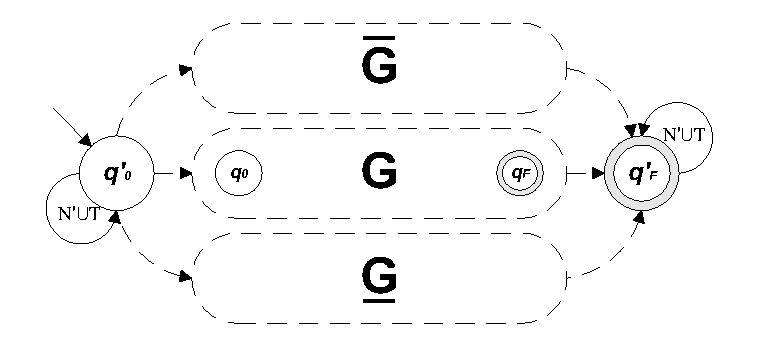
\includegraphics{img/gsystems/g_s_p_1}
      \caption{1-$a$-prekladač $g$-systému $G'$} \label{gs_obr_gsp1}
    \end{figure}

    Na to, aby sme mali $L(G)=L(G')$ ešte potrebujeme v istom kroku
    odznačiť prvý aj posledný označený symbol. Avšak keďže máme v
    1-$a$-prekladači $g$-systému $G'$ šípky z $q'_0$ do iného stavu,
    resp. šípky do $q'_F$ z iného stavu (teda nie kopírovacie cykly v
    týchto stavoch) iba na označený symbol, tak s odznačenou vetnou
    formou už ďalej nepohneme. Z toho plynie, že symboly možno
    odznačiť len v poslednom kroku odvodenia, teda vtedy, ak všetky
    symboly vetnej formy, okrem prvého a posledného, sú terminály a aj
    prvý a posledný symbol (odhliadnuc od označenia) sú terminály.
    Teda opäť nedeterministicky hádame posledný krok. Formálne
    definujme:
    \[
    H_T=\{(q'_0,\overline{a},a,q_T),(q_T,a,a,q_T),
    (q_T,\underline{a},a,q'_F)\mm a\in T\}
    \]
    $q_T$ je nový stav 1-$a$-prekladača $g$-systému $G'$. Zachovali
    sme konzistentnosť v tom zmysle, že z $q'_0$ vychádzajú, okrem
    kopírovacích cyklov, iba šípky na prvý (nad\-čiar\-knu\-tý) symbol
    a do $q'_F$ vchádzajú, okrem kopírovacích cyklov, iba šípky na
    posledný\linebreak (pod\-čiar\-knu\-tý) symbol vetnej formy, teda máme
    $L(G)=L(G')$, pričom\newline $G'=(N',T,M',\underline{\overline{\sigma}})$.
    Čo sa týka $M'$ pre nás je zaujímavé, ako sa zmenila prechodová
    množina: keď v $M$ to bola $H$, tak v $M'$ to bude
    $H_{M'}=H'\cup\overline{H}\cup\underline{H}\cup H_T$. Pokiaľ ide o
    stavy a abecedy, ich konštrukcia by mala byť z už uvedeného
    zrejmá.
  \end{enumerate}
  \item Ku $G'=(N',T,M',\underline{\overline{\sigma}})$
  zostrojíme ekvivalentný $g$-systém $G''$ tak, že prerušíme všetky vnútorné cykly
  (teda tie, ktoré nie sú kopírovacie v počiatočnom alebo koncovom
  stave). Vonkajšou šípkou 1-$a$-prekladača nazveme takú, ktorá buď
  vychádza z počiatočného stavu, alebo vchádza do akceptačného stavu
  (v našom prípade ide o stavy $q'_0,q'_F$). Ostatné šípky nazveme
  vnútorné. Pri odstraňovaní cyklov budeme postupovať nasledovne:
  \begin{enumerate}
    \item stavy budú rovnaké ako v $G'$
    \item všetky vonkajšie šípky necháme tak ako sú
    \item každú vnútornú šípku nahradíme dvoma novými nasledovne: ak
    $(q,a,u,p)\in H_{M'}$, tak $(q,a,u,p)\not\in H_{M''},
    (q,a,[q,a,u,p],q'_{F})\in H_{M''}, (q'_0,[q,a,u,p],u,p)\in
    H_{M''}$, pričom $[q,a,u,p]$ budú nové neterminály\footnote{Ak sa
    čitateľ trochu zamyslí, malo by mu byť jasné, že v každom kroku
    môže byť vo vetnej forme najviac jeden takýto neterminál}
    (obr.\ref{gs_obr_gps2})
  \end{enumerate}

  \begin{figure}[!ht]
    \centering
    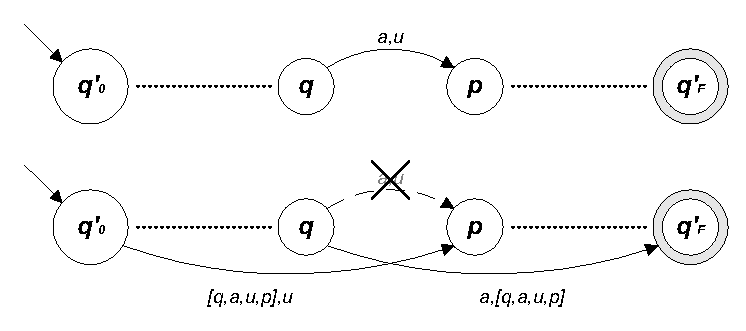
\includegraphics{img/gsystems/g_s_p_2}
    \caption{Nahrádzanie vnútorných šípok v $G''$} \label{gs_obr_gps2}
  \end{figure}

  Môže sa naskytnúť otázka: prečo sme nenahradzovali aj vonkajšie
  šípky? Odpoveď je veľmi jednoduchá: pretože ony žiadne cykly
  vytvárať nemohli, tak sme $G'$ konštruovali. Malo by byť zrejmé,
  že takto sme odstránili všetky cykly, okrem kopírovacích v
  počiatočnom a koncovom stave, lebo teraz všetky šípky vychádzajú z
  $q'_0$ alebo vchádzajú do $q'_F$ a toto sú jediné šípky v $G''$.
  Rovnako zrejmé by malo byť $L(G')=L(G'')$, v $G''$ sme iba
  nahradili jeden paralelný krok $n$ sekvenčnými, kde $n$ je počet
  šípok v jednom paralelnom kroku.
\end{enumerate}
Máme zkonštruovaný $g$-systém $G''$ taký, že $L(G)=L(G'')$ a
$G''\in\mathcal{S}$, teda naše ``zosekvenčňovanie'' $g$-systému
$G$ je na konci.
\end{dokaz}

Nasledujúce tvrdenia hovoria niečo o zložitosti $g$-systému ktorý
sme práve zostrojili v pred\-chá\-dza\-jú\-cej konštrukcii a
priamo z nej vyplývajú.

\begin{veta}
(Vzťah popisnej zložitosti sekvenčných a paralelných $g$-systémov)
\begin{itemize}
  \item $\forall L\med STATE_{\mathcal{S}}(L)\leq
  3.STATE_{\mathcal{G}}(L)+3$
  \item $ARC_{\mathcal{S}}(L)\leq 32.STATE_{\mathcal{G}}(L)+22.\#\Sigma_L$
\end{itemize}
\end{veta}

Je dobré si uvedomiť, že zosekvenčnením $g$-systému sme nepoužili
žiadny priestor navyše, o čom hovorí nasledujúca veta.

\begin{veta}
$SPACE_{\mathcal{S}}(f(n))=SPACE_{\mathcal{G}}(f(n))$ pre $\forall
f(n)$
\end{veta}

\begin{veta}\label{gs_veta_h_odhad}
Pre ľubovoľný jazyk $L$ a ľubovoľný
$G\in\mathcal{G}$ taký, že $L=L(G)$ platí:
\[
L\in
TIME_{\mathcal{S}}(SPACE_{\mathcal{G}}(G,n).TIME_{\mathcal{G}}(G,n))
\]
\end{veta}

Veta \ref{gs_veta_h_odhad} hovorí o akomsi hornom odhade počtu  krokov
sekvenčných \mbox{$g$-sys}té\-mov v porovnaní\linebreak s
paralelnými. Na bližšie pochopenie tohto tvrdenia si stačí
uvedomiť, že sekvenčný $g$-systém môže v jednom kroku vďaka tomu,
že nemá vnútorné cykly, prepísať len istý, vo všeobecnosti malý,
úsek vetnej formy na rozdiel od paralelného $g$-systému, ktorý
môže v jednom kroku prepísať celú vetnú formu. Teda ak chce
sekvenčný $g$-systém odsimulovať jeden krok paralelného\linebreak
$g$-systému, musí urobiť $\{$ rádovo dĺžka vetnej formy $\}$
krokov. Ak chceme sekvenčne odsimulovať celý výpočet paralelného
$g$-systému, dostávame spomínané tvrdenie.

\smallskip
Keď sa na tento problém pozrieme z opačnej strany (keď chceme
jazyk generovaný sekvenčným $g$-systémom, generovať paralelným
$g$-systémom), podobná úvaha nám umožňuje pretransformovať dolný
odhad počtu krokov pre sekvenčné $g$-systémy na dolný odhad počtu
krokov pre paralelné $g$-systémy. Dostávame teda nasledujúce
tvrdenie.

\begin{veta}
\label{gs_veta_d_odhad}
$\overline{TIME}_{\mathcal{S_{\varepsilon}}}(f(n))\subseteq
\overline{TIME}_{\mathcal{G_{\varepsilon}}}(\frac{f(n)}{n})$
\end{veta}

Toto tvrdenie nám ukazuje, že vzťah paralelných a sekvenčných
$g$-systémov je lineárny a teda, že paralelizmus nám vo
všeobecnosti veľmi nepomôže (aspoň nie nejak dramaticky), ako si
však neskôr ukážeme, existujú tzv. ``rýchlo generovateľné''
jazyky, kde je rozdiel výraznejší.

\begin{priklad}
Je známe, že $L=\{wcw\mm
w\in\{a,b\}^*\}\in\overline{TIME}_{\mathcal{S_{\varepsilon}}}(n^2)$,
teda podľa vety \ref{gs_veta_d_odhad} $L\in
TIME_{\mathcal{G_{\varepsilon}}}(n)$. Paralelizmus teda tomuto
jazyku veľmi nepomôže, nie je totiž exponenciálny
\end{priklad}

\section{Normálové tvary $g$-systémov}

\begin{definicia}
Hovoríme, že $g$-systém je v normálovom tvare, ak spĺňa
nasledujúce podmienky:
\begin{enumerate}
\item existuje kopírovací cyklus pre $\forall a\in N\cup T$ v $q_0$ aj v $q_F$
\item iba kopírovacie cykly vstupujú do $q_0$ a vystupujú z $q_F$
\item terminálne symboly sa iba kopírujú
\item $g$-systém je bez $\varepsilon$
\end{enumerate}
\end{definicia}

\begin{oznacenie}
$\mathcal{N}$ je trieda všetkých $g$-systémov v normálnom tvare
\end{oznacenie}

\begin{veta}
$\mathcal{L}_{\mathcal{N}}=\mathcal{L}_{\mathcal{G}_{\varepsilon}}$
\end{veta}

\begin{dokaz}
Inklúzia $\subseteq$ je zrejmá vďaka štvrtej podmienke. Dokážeme
opačnú inklúziu: \\ Nech
$G=(N,T,M,\sigma)\in\mathcal{G}_\varepsilon$. Chceme zostrojiť
$G''\in\mathcal{N}$ taký, že $L(G'')=L(G)$, teda chceme. aby $G''$
spĺňal všetky štyri podmienky z definície $\mathcal{N}$. Keďže
$G\in\mathcal{G}_\varepsilon$ tak podmienka 4 je automaticky
splnená. $G''$ zostrojíme v dvoch krokoch:
\begin{enumerate}
  \item Najskôr zostrojíme $G'=(N',T,M',\sigma)$ taký, že $L(G')=L(G)$ a $G'$ bude
  spĺňať tretiu podmienku z definície $\mathcal{N}$:
  \begin{itemize}
    \item $N'=N\cup\{\xi_a\mm a\in T\}$
    \item $\forall a\in T$ : všetky výskyty
    terminálu $a$ v $H$ nahradíme novým neterminálom $\xi_a$
    \item v $q_0$ nedeterministicky uhádneme, že vetná forma
    obsahuje už len neterminály typu $\xi_a$ a celú ju
    zterminálnime. Do $M'$ pridáme nový stav $q'$ a do $H'$
    pridáme štvorice: pre $\forall\; a\in T$ $(q_0,\xi_a,a,q')$
    a $(q',\xi_a,a,q')$, pričom $q'$ bude akceptačným stavom.
  \end{itemize}
  \item Na $G'$ použijeme konštrukciu podobnú s prvou časťou
  konštrukcie z kapitoly \ref{gs_sec_sekvspar}, ktorá nám zabezpečí
  splnenie podmienok 1 a 2. Všimnime si, že keďže pracujeme s bez
  $\varepsilon$ $g$-sytémami, tak nemusíme strojnásobovať stavy, a
  teda vychádzajú aj lepšie odhady popisnej zložitosti.
\end{enumerate}
\end{dokaz}

\begin{dosledok}
Pre každý jazyk $L\in\mathcal{L}_{\mathcal{G}_{\varepsilon}}$
platí:
\begin{enumerate}
  \item $STATE_{\mathcal{N}}(L)\leq STATE_{\mathcal{G}_{\mathcal{\varepsilon}}}(L)+3$
  \item $ARC_{\mathcal{N}}(L)\leq 12.ARC_{\mathcal{G}_{\varepsilon}}(L)+14.\#\Sigma_L$
  \item $SPACE_{\mathcal{N}}(n)=SPACE_{\mathcal{G}_{\varepsilon}}(n)=\mathcal{L}_{CS}$
  \item $TIME_{\mathcal{N}}(f(n))=TIME_{\mathcal{G}_{\varepsilon}}(f(n))$
\end{enumerate}
\end{dosledok}

\begin{oznacenie}
$STATE_{\mathcal{N}}(n)=\{ L\mm\exists G\in\mathcal{N}, STATE(G)\leq n, L=L(G)\}$
\end{oznacenie}

\begin{veta}
$STATE_{\mathcal{N}}(n)$ je $\mathcal{AFL}$ pre\footnote{pre $n=1$ by boli problémy s
$h^{-1}$} $\forall n>1$
\end{veta}

\begin{oznacenie}
$\mathcal{N}_{i,j}$ - trieda všetkých sekvenčných $g$-systémov v
normálnom tvare, ktoré majú najviac $i$ stavov a najviac $j$
neterminálov, pričom sú dovolené $\varepsilon$ prechody v
1-$a$-prekladači.
\end{oznacenie}

\pagebreak

\begin{veta}
$\mathcal{L}_{\mathcal{N}_{6,2}}=\mathcal{L}_{\mathcal{N}_{5,3}}=\mathcal{L}_{\mathcal{N}_{4,4}}=\mathcal{L}_{RE}$
\end{veta}

Pre $\mathcal{N}_{6,2}$ tvrdenie platí, ak $g$-systém začína svoju
prácu z počiatočného slova, otvoreným\linebreak problémom je, či
platí aj pri použití počiatočného neterminálu.

\medskip
Dôsledkom tejto vety sú niektoré normálové tvary pre frázové
gramatiky:

\begin{dosledok}
K ľubovoľnému jazyku $L\in\mathcal{L}_{RE}$ existuje taká frázová
gramatika, že všetky jej pravidlá sú tvaru:
\begin{enumerate}
  \item $\sigma\ra u$ alebo $AB\ra\varepsilon$ a $CD\ra\varepsilon$ kde $N=\{\sigma
  ,A,B,C,D\}$ a $u\in (N\cup T)^*$
  \item $\sigma\ra u$ alebo $ABBBA\ra\varepsilon$ kde $N=\{\sigma ,A,B\}$ a $u\in (N\cup T)^*$
  \item $\sigma\ra u$ alebo $ABC\ra\varepsilon$ kde $N=\{\sigma ,A,B,C\}$ a $u\in (N\cup T)^*$
\end{enumerate}
\end{dosledok}

Otvorenými problémami zostávajú:
\begin{itemize}
  \item $\mathcal{N}_{5,2}\overset{?}{=}\mathcal{L}_{RE}$
  \item $\mathcal{N}_{4,2}\overset{?}{=}\mathcal{L}_{RE}$
  \item $\mathcal{N}_{4,3}\overset{?}{=}\mathcal{L}_{RE}$
\end{itemize}

\section{Charakterizácia triedy $TIME_{\mathcal{G}}(f(n))$ pomocou
sek\-venč\-ného priestoru}

\begin{definicia}
Nech $D$ je odvodenie slova $w\in L(G)$ $g$-systémom
$G=(N,T,M,\sigma)$, kde $M=(K,\Sigma,\Sigma,H,q_0,q_F)$. Strom
odvodenia (ozn. $T_D$) nazývame strom, ktorého vrcholy sú označené
ako štvorice z $H$, pričom označenie koreňa $T_D$ je tvaru
$(q_0,\sigma,u,q_F)$, kde $u\in (N\cup T)^*$. Vrchol s označením
$(q,a,b_1b_2\dots b_k,p)$ má $k$ synov $(p_1,b_1,u_1,p_2)
(p_2,b_2,u_2,p_3)\dots(p_k,b_k,u_k,p_{k+1})$, kde $\forall i
u_i\in (N\cup T)^*$. Postupnosť štvoríc na každej úrovni stromu je
výpočet 1-$a$-prekladača. Zreťazením tretích komponent štvoríc na
$k$-tej úrovni dostaneme $k$-tu vetnú formu výpočtu $G$. Teda
zreťazením tretích komponent štvoríc na poslednej
úrovni\footnote{hĺbka stromu odvodenia $\geq TIME(G,w)$} dostaneme
slovo $w$.
\end{definicia}

\begin{priklad}
Zoberme si $g$-systém a jeho 1-$a$-prekladač pre jazyk $L=\{ww\mm
w\in\{a,b\}^* \}$ \mbox{z príkladu} \ref{gs_prikl_aprekladac}. Zoberme si
jedno konkrétne odvodenie $S\Ra AA\Ra aAaA\Ra abab$. Jednotlivým
krokom tohto odvodenia zodpovedá v 1-$a$-prekladači výpočet:
\begin{itemize}
  \item $S\Ra AA\rightsquigarrow (q_0,S,AA,q_F)$
  \item $AA\Ra aAaA\rightsquigarrow (q_0,A,aA,q_1)(q_1,A,aA,q_F)$
  \item $aAaA\Ra abab\rightsquigarrow
  (q_0,a,a,q_0)(q_0,A,b,q_4)(q_4,a,a,q_4)(q_4,A,b,q_F)$
\end{itemize}
Strom tohto odvodenia je na obrázku \ref{gs_obr_stromodv}.
\end{priklad}

\pagebreak

\begin{figure}[!ht]
  \centering
  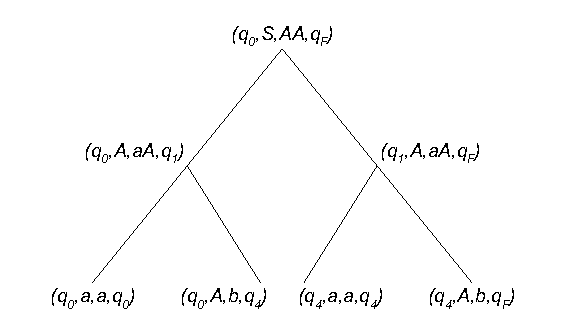
\includegraphics{img/gsystems/stromodv}
  \caption{Strom zodpovedajúci odvodeniu $S\Ra AA\Ra aAaA\Ra abab$}
  \label{gs_obr_stromodv}
\end{figure}

\begin{lema}
$TIME_{\mathcal{G}}(f(n))\subseteq 1NSPACE(f(n))$ pre $\forall
f(n)$.
\end{lema}

\begin{dokaz}
Nech $G=(N,T,M,\sigma)$ je $g$-systém pracujúci v čase $O(f(n))$.
Chceme skonštruovať Turingov stroj $A$ s jednosmernou vstupnou
páskou, ktorý bude simulovať $G$ v priestore $O(f(n))$. Uvažujme
slovo $w\in L(G)$ a jeho príslušný strom odvodenia $T$. Chceme
ukázať, že $A$ akceptuje $w$ práve vtedy, keď $w\in L(G)$.  $A$
bude na svojej pracovnej páske zapisovať cesty z $T$ vedúce od
koreňa k listom (obr.\ref{gs_obr_nspace}). $A$ bude hádať tieto cesty a
overovať, či jednotlivé štvorice na rovnakej úrovni $T$ tvoria
výpočet 1-$a$-prekladača $M$ a či zreťazenie výstupov štvoríc v
listoch $T$ tvoria $w$.

\begin{figure}[!ht]
\centering
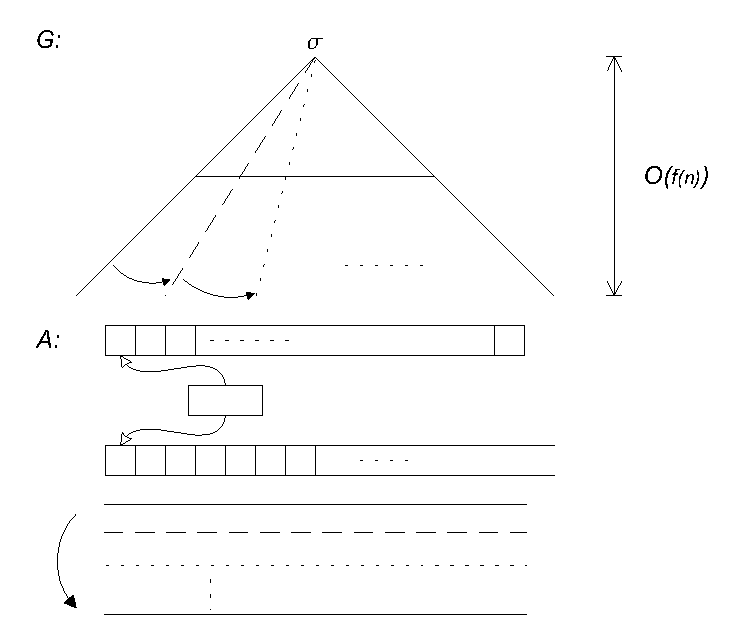
\includegraphics{img/gsystems/nspace}
\caption{Simulácia $g$-systému $G$ Turingovým strojom $A$}
\label{gs_obr_nspace}
\end{figure}

$A$ najprv uhádne a zapíše na pracovnú pásku cestu z koreňa do
najľavejšieho listu $\alpha$, pričom musí skontrolovať či prvá
štvorica je tvaru $(q_0,\sigma,u,q_F)$ a ostatné štvorice musia
začinať v stave $q_0$ a prepisovať prvý symbol výstupu
predchádzajúcej štvorice. Naviac výstup listu $\alpha$ musí byť
prefixom slova $w$. Ak nejaká z týchto podmienok neplatí, tak $A$
neuhádol najľavejšiu cestu správne a zasekne sa. Ak $A$ uhádol,
tak nahradí štvoricu $\alpha$ jeho najľavejším bratom $\beta$ (to
samozrejme tiež uhádne (obr.\ref{gs_obr_nstrom}a) a zaznačí si, že
$\beta$ je druhým synom ich spoločného otca $\gamma$. $A$ overí,
či $\beta$ je dobre uhádnutý t.j. počiatočný stav $\beta$ je
rovnaký ako koncový stav $\alpha$,  $\beta$ prepisuje druhý symbol
výstupu $\gamma$ a výstup $\beta$ je rovnaký ako ďalšia časť $w$
(bez prefixu, ktorý bol vo výstupe $\alpha$). Takto $A$ pokračuje
až kým neuhádne a neoverí posledného syna $\gamma$. Potom $A$
nahradí $\gamma$ jeho najľavejším bratom $\delta$ (podobne ako bol
$\alpha$ nahradený $\beta$). Teda $A$ robí prehľadávanie do hĺbky,
pričom si treba uvedomiť, že pri návrate na vyššiu úroveň v
strome, si $A$ musí pamätať koncové stavy jednotlivých vrcholov,
aby mohol pri hádaní ďalších vrcholov overiť správnu následnosť.

\begin{figure}[!ht]
\centering
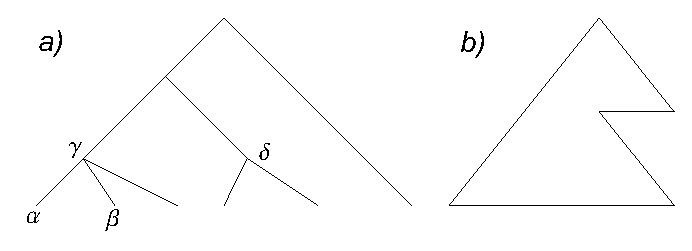
\includegraphics{img/gsystems/nstrom}
\caption{Nahrádzanie hrán v 1-$a$-prekladači $M$} \label{gs_obr_nstrom}
\end{figure}

Týmto spôsobom $A$ pokračuje až kým vo výstupoch listov nenájde
celé slovo $w$. Potom už $A$ vie, že všetky ostatné neoverené
listy musia mať na výstupe $\varepsilon$ (obr.\ref{gs_obr_nstrom}b). Teda
zvyšné cesty bude $A$ hľadať s tým, že v listoch musí byť na
výstupe $\varepsilon$. Keď $A$ dosiahol najpravejší list (to je,
ako inak, opäť uhádnuté), tak $A$ overí či všetky koncové stavy vo
všetkých štvoriciach na celej pracovnej páske sú $q_F$. Ak je to
tak, potom $A$ akceptuje $w$.

Z konštrukcie $A$ je zrejmé, že $A$ akceptuje $w$ práve vtedy, keď
$w\in L(G)$. Keďže $w\in L(G)$, tak hĺbka stromu odvodenia nie je
väčšia ako $c.f(|w|)$ kde $c$ je konštanta nezávislá od $w$, teda
hĺbka stromu odvodenia je $O(f(n))$, a teda $A$ na akceptovanie
slova $w$ nepotrebuje viac políčok na páske ako $O(f(n))$ z čoho
konečne plynie, že $L(G)\in 1NSPACE(f(n))$.
\end{dokaz}

\begin{lema}
$1NSPACE(f(n))\subseteq TIME_{\mathcal{G}}(f(n))$ pre $f(n)=\Omega
(\log n)$.
\end{lema}

\begin{dokaz}
Nech $A$ je nedeterministický Turingov stroj s jednosmernou
vstupnou páskou, ktorý akceptuje v priestore $O(f(n))$. Bez ujmy
na všeobecnosti predpokladajme, že $A$ má len jednu jednosmerne
nekonečnú pracovnú pásku.

Očíslujme políčka pracovnej pásky 0,1,2\dots Chceme skonštruovať
$g$-systém $G$, ktorý simuluje $A$ v čase $O(f(n))$. Jedna vetná
forma $G$ obsahuje informáciu o políčku pracovnej pásky $A$ počas
celého výpočtu. Nasledujúca vetá forma obsahuje informáciu o
nasledujúcom políčku atď. Keďže $A$ pracuje na najviac $O(f(n))$
políčkach, tak $G$ potrebuje na vygenerovanie slova dĺžky $n$
najviac $O(f(n))$ vetných foriem (t.j. $G$ pracuje v čase
$O(f(n))$). Samozrejme $G$ musí zaručiť konzistentnosť medzi
jednotlivými políčkami pásky, stavmi $A$ a symbolmi na vstupnej
páske podľa $\delta$-funkcie $A$.

Uvažujme jeden výpočet $A$ na vstupnom slove $w\in L(A)$. Nech $s$
je priestor a $t$ je čas potrebný na výpočet $w$. Odvodenie slova
$w$ $g$-systémom $G$ je tvaru:

\centerline{$\sigma =w_0\overset{k}\Ra w_k\Ra w_k'\Ra w_{k+1}\Ra
w_{k+1}'\Ra\dots\Ra w_{k+s}\Ra w_{k+s}'\Ra w$} kde vetná forma
$w_{k+j}$ drží obsah $j$-teho a $j+1$. políčka $A$ v celom výpočte
$A(w)$ a vetná forma $w_{k+j}'$ je použitá na overenie či uhádnuté
obsahy sú legálne vzhľadom na $\delta$-funkciu $A$.\\ $i$-ty
symbol vetnej formy $w_{k+j}$ je päťposchodový symbol obsahujúci:

\begin{itemize}
  \item stav $p_i$, v ktorom je $A$ v čase $i$ ($p_{t+1}$ je akceptujúci)
  \item symbol $a_i$, ktorý v čase $i$ číta vstupná hlava $A$, pričom tento symbol si
  označíme, ak v čase $i$ $A$ posúva hlavu na vstupe
  \item symbol $b_{j,i}$, ktorý je na $j$-tom políčku pracovnej pásky $A$ v čase $i$
  \item symbol $b_{j+1,i}$, ktorý je na $j+1$. políčku pracovnej pásky $A$ v čase $i$
  \item špeciálny symbol $0$, ak hlava bola na $j$-tom políčku, špeciálny symbol $1$, ak
  hlava bola na $j+1$. políčku a v ostatných prípadoch špeciálny
  symbol -
\end{itemize}

V prvých $k$-krokoch $G$ odvodí (uhádne\footnote{to sa dá na
$O(f(|w|))$ krokov keďže $A$ pracuje v priestore $O(f(|w|))$ a
teda v čase $O(|w|.c^{f(|w|)})$ pre nejakú konštantu $c$ t.j.
počet všetkých možných konfigurácií $A$ pri výpočte $w$. $g$-systém vie toľkoto
symbolov vygenerovať v logaritmickom čase, čo je v tomto prípade $O(f|w|)$.}) vetnú
formu $w_k$ dĺžky $t+1$ t.j. postupnosť stavov, ktorými $A$
prechádza počas výpočtu na $w$, vstupné slovo a časy, v ktorých
$A$ pohne hlavou na vstupe, obsahy nultého a prvého políčka
pracovnej pásky $A$ počas celého výpočtu a časy výskytu hlavy na
nultom políčku pracovnej pásky. Schématicky vyzerá vetná forma ako
na obrázku \ref{gs_obr_time_g}.

\begin{figure}[!ht]
  \centering
  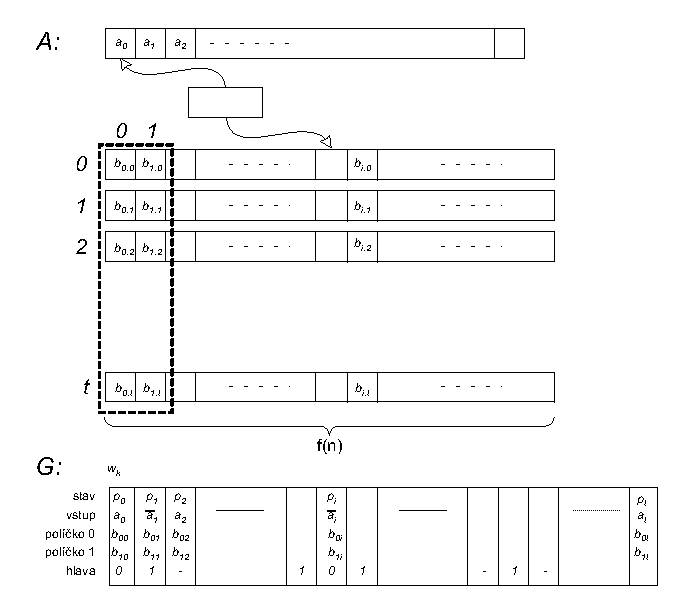
\includegraphics{img/gsystems/time_g}
  \caption{Simulácia TS $A$ $g$-systémom $G$} \label{gs_obr_time_g}
\end{figure}

V kroku $k+1$ $G$ overí či, to čo uhádol v predchádzajúcom kroku
je v súlade s $\delta$-funkciou $A$ a vygeneruje\footnote{tento
krok je naozaj iba overovací, to znamená, že ak $G$ uhádol dobre,
tak $w_k'=w_k$ inak sa $G$ zasekne} $w_k'$. Ak to bolo uhádnuté
dobre, tak $G$ vygeneruje $w_{k+1}$ t.j. prvé a druhé poschodie
bude rovnaké ako v $w_k'$, štvrté poschodie $w_k'$ bude vo
$w_{k+1}$ tretím poschodím, a kde bol v piatom poschodí $w_k'$
špeciálny symbol $1$, tam bude v piatom poschodí $w_{k+1}$
špeciálny symbol $0$, ostatné $G$ uhádne\footnote{t.j. $G$ uhádne
symboly na druhom políčku pracovnej pásky $A$ počas celého výpočtu
a časy výskytu hlavy na prvom políčku} (obr.\ref{gs_obr_time_g2}). V
ďalšom kroku $G$ overí či to čo uhádol teraz je legálne vzhľadom
na $\delta$-funkciu $A$ a vygeneruje $w_{k+1}'$\dots

Overovanie vo všeobecnosti vyzerá tak, že $G$ akoby sa naraz
pozeral na dva susedné päťposchodové symboly, takže vidí isté malé
okolie (2 symboly) pracovnej pásky v istom malom časovom úseku (2
takty TS) a k zmenám na pracovnej páske hľadá príslušnú časť
$\delta$-funkcie, ktorá je schopná takéto zmeny spôsobiť. Ak
takúto časť $\delta$-funkcie $A$ nájde, tak tieto dva
päťposchodové symboly môžu stáť vedľa seba a $G$ sa posunie o
jeden päťposchodový symbol. Takto môže $G$ overiť celú vetnú
formu.

$G$ pokračuje v striedaní hádacích a overovacích krokov, až kým
neodvodí vetnú formu bez špeciálnych symbolov výskytu hlavy na
pracovnej páske $A$ t.j. v piatom poschodí vetnej formy sa
nevyskytuje $0$ ani $1$. To znamená, že $G$ odsimuloval celý
výpočet $A$.

\begin{figure}[!ht]
  \centering
  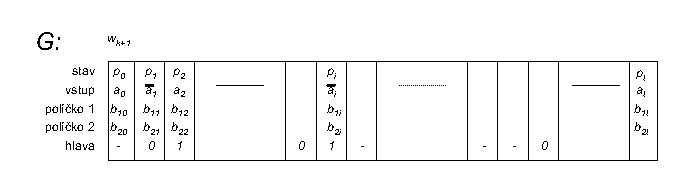
\includegraphics{img/gsystems/time_g2}
  \caption{Posun symbolov vo vetnej forme} \label{gs_obr_time_g2}
\end{figure}

V poslednom kroku $G$ prepíše vetnú formu tak, že každý
päťposchodoví symbol sa prepíše na symbol z druhého poschodia
(t.j. symbol zo vstupnej pásky $A$) ak bol tento symbol označený,
inak sa celý päťposchodový symbol prepíše na $\varepsilon$.

Zrejme $w\in L(G)\Longleftrightarrow$ ak $w$ je akceptované $A$.
Naviac $w$ je vygenerované v čase\newline
$O(f(n))+O(2f(n))=O(f(n))$. Samozrejme dva kroky odvodenia $G$
$w_l\Ra w_l'\Ra w_{l+1}$ sa dajú nahradiť jedným, potom $w$ je
vygenerované v čase $O(f(n))+O(f(n))=O(f(n))$. Tento spôsob
odvodenia sme zvolili iba pre lepšiu čitateľnosť dôkazu.
\end{dokaz}

\medskip
Predchádzajúce dve lemy nám umožňujú vysloviť nasledujúce tvrdenie:

\begin{veta}
$TIME_{\mathcal{G}}(f(n))=1NSPACE(f(n))$ pre $f(n)\geq\log n$.
\end{veta}

Ak si uvedomíme, že pre $f(n)\geq n$ je pracovná páska Turingovho
stroja dosť dlhá, aby sme si na nej zapamätali vstup, potom
$1NSPACE(f(n))=NSPACE(f(n))$.

Ďalším jednoduchým pozorovaním zistíme, že ak $f(n)\geq n$, tak
priestor na $TS$ a na $g$-systémoch je ekvivalentný, teda
$NSPACE(f(n))=SPACE_{\mathcal{G}}(f(n))$.

Môžeme teda vysloviť nasledovné dôsledky predchádzajúcej vety:

\begin{dosledok}
$TIME_{\mathcal{G}}(f(n))=NSPACE(f(n))$ pre $f(n)\geq n$.
\end{dosledok}

\begin{dosledok}
$TIME_{\mathcal{G}}(f(n))=SPACE_{\mathcal{G}}(f(n))$ pre $f(n)\geq
n$.
\end{dosledok}

\pagebreak

\section{Niektoré vlastnosti ``rýchlo generovateľných'' jazykov}

``Rýchlo generovateľné'' jazyky nazývame také jazyky z triedy
$TIME_{\mathcal{G}}(f(n))$, pre ktoré $f(n)<n$.

\begin{veta}
$TIME_{\mathcal{G}}(\log^p n)$ je $\mathcal{AFL}$
pre\footnote{rýchlejšie ako v logaritmickom čase $g$-systém
nedokáže pracovať} $p\geq 1$.
\end{veta}

\begin{veta}
$TIME_{\mathcal{G}}(\log^p n)\subsetneq TIME_{\mathcal{G}}(\log^q
n)$ pre $q>p>1$.
\end{veta}

\begin{dosledok}
Hierarchia $TIME_{\mathcal{G}}(\log^p n)$ pre $p>1$ je nekonečná.
\end{dosledok}

\begin{veta}
Pre každý jazyk $L\in\mathcal{L}_{RE}$ existuje $L'\in
TIME_{\mathcal{G}}(\log n)$ a existuje homomorfizmus $h$ taký, že
$L=h(L')$.
\end{veta}

\begin{dokaz}
Táto veta nám hovorí, že ku každému jazyku $L\in\mathcal{L}_{RE}$
vieme nájsť $g$-systém $G$ pracujúci v logaritmickom čase a
homomorfizmus $h$ taký, že $h(L(G))=L$. Veta \ref{gs_veta_gre} nám
hovorí, že vieme k $L$ nájsť príslušný $g$-systém $G$, ale
nezaručuje, že bude pracovať v logaritmickom čase. $G$ upravíme na
$G'$ nasledovne:
\begin{itemize}
\item Do 1-$a$-prekladača $G$ zavedieme nový terminál $\gamma$
\item Každú štvoricu tvaru $(q_0,\sigma ,u,p)$ nahradíme štvoricou $(q_0,\sigma ,\gamma u,p)$
\item Pridáme štvoricu $(q_0,\gamma,\gamma\gamma,q_0)$
\end{itemize}
Ľahko vidno, že takto upravený $g$-systém $G'$ generuje jazyk

\centerline{$L'=\{\gamma^{2^m} w\mm w\in L(G)$ a $m$ je počet
krokov odvodenia $w$ v $G\}$} Zamyslime sa teraz nad časovou
zložitosťou $G'$. Zoberme si nejaké slovo $u=w{\gamma}^{2^k}\in
L'$ pre nejaké $k$. Zrejme $|u|\geq 2^k$, ale $G'$ toto slovo
vygeneruje v $k$ krokoch, teda v logaritmickom čase, a teda $L'\in
TIME_{\mathcal{G}}(\log n)$. Homomorfizmus $h$ zvolíme takto:
\begin{itemize}
\item $\forall a\in T: h(a)=a$
\item $h(\gamma)=\varepsilon$
\end{itemize}
To znamená, že $h$ vymaže všetky $\gamma$ zo slov $w\in L'$, ktoré
sme zaviedli $g$-systémom $G'$. Teda $h(L')=L$. Ak sa nad touto
konštrukciou ešte raz zamyslíme, zistíme, že my sme $g$-systém
nejakým spôsobom ``nezrýchľovali'', ale to, že sme jazyk dostali
do logaritmickej časovej zložitosti sme dosiahli tým, že dĺžku
slov z tohto jazyka sme natoľko zväčšili, že pri zachovaní počtu
krokov odvodenia bude tento jazyk vygenerovaný v logaritmickom
čase vzhľadom na túto zväčšenú dĺžku slova.
\end{dokaz}

\begin{dosledok}
Trieda $TIME_{G}(f(n))$ nie je uzavretá na ľubovoľný
homomorfizmus.
\end{dosledok}

\section{Záverom o $g$-systémoch}

Je vhodné si uvedomiť niekoľko významných faktov, ktoré nám model
generatívnych systémov priniesol.

Pre známe paralelné gramatiky, ktoré dokážeme simulovať na
$g$-systémoch, dostaneme priestorové ohraničenie najviac
$1NSPACE(f(n))$. Podobne, ak navrhneme nový paralelný model, ktorý
vieme ``tesne'' simulovať na $g$-systémoch, dostaneme priestorové
ohraničenie $1NSPACE(f(n))$. Naviac pre každý jazyk $L\in
1NSPACE(f(n))$ existuje nejaký typ paralelnej gramatiky, ktorá $L$
dokáže generovať v čase $f(n)$.

\chapter{Kooperujúce distribuované systémy gramatík ($CDGS$)}

V tejto kapitole ukážeme ďalšiu možnosť paralelizmu, kde viac gramatík pracuje na jednej
spoločnej vetnej forme: gramatika dostane vetnú formu a pracuje na nej tak dlho, ako je
jej určené...

\begin{definicia}
$CDGS$ je $(n+2)$-tica $\Gamma = (T,G_1,G_2,...,G_n,S)$, kde $ \forall i G_i = (
N_i,T_i,P_i)$ je "bezkontextová gramatika bez počiatočného symbolu". $T\subseteq
\underset{i}\bigcup T_i$ , $S \in \underset{i}\bigcup N_i$ je počiatočný symbol
\end{definicia}

\begin{definicia}
Nech $\Gamma = (T,G_1,G_2,...,G_n,S)$. Krok odvodenia je relácia $\krok{\leq k}{\Gamma}$,
kde $\krok{\leq k}{\Gamma}\med = \med\krok{\leq k}{G_i}i\in \{1,2,...,n\}$
definovaná nasledovne: $\krok{\leq k}{G_i}\med =\med (\underset{j=1} {\overset{k}\bigcup}
 \krok{j}{G_i})$, podobne definujeme aj: $\krok{\geq k}{\Gamma}$, $\krok{=k}{\Gamma} $.
Definujeme $x\krok{\widetilde{t}}{\Gamma}y$\footnote{ďalej budeme písať len $x
\krok{t}{\Gamma}y$ }: $x\krok{t}{\Gamma}y$ = $x\krok{t}{G_i} y\med i\in \{1,2,...n\}$
platí práve vtedy, ak: $x \krok{*}{G_i}y$ a $\not\exists z \not = y:
y\underset{G_i}\Ra z$
\end{definicia}

\begin{definicia}
Nech $f \in \{ t,*,=1,=2,...,\leq 1,\leq 2,...,\geq 1,\geq 2,...\}$ a nech $\Gamma$ je
$CDGS$. Potom jazyk definovaný systémom pri spôsobe prepisovania $f$ je
\[
L_f(\Gamma)=\{w \in T^* \mm \exists r,i_1,i_2,...,i_r\med S\krok{f}{G_{i_1}}w_1
\krok{f}{G_{i_2}}w_2 \krok{f}{G_{i_3}}...\krok{f}{G_{i_r}}w_r\equiv w\}
\]
\end{definicia}

\begin{priklad}
$\Gamma = (\{a,b,c\},G_1,G_2,S)$\\ $G_1 = (\{A,B\},\{A',B',a,b,c\},\{A\ra aA'b,B\ra
cB',A\ra ab, B\ra c\})$ a\\
$G_2 = (\{S,S',A',B'\},\{A,B\},\{S\ra S',S'\ra AB,A'\ra A,
B'\ra B\})$, potom
\begin{description}
\item{}$L_{=1}(\Gamma)=L_{*}(\Gamma)=L_{\leq k}(\Gamma)=L_{\geq 1}(\Gamma)=L_{t}(\Gamma)=
\{a^n b^n c^m \mm n,m\geq 1\}, k\geq 1$
\item{}$L_{=2}(\Gamma)=L_{\geq 2}(\Gamma)=\{a^n b^n c^n \mm n\geq 1 \}$
\item{}$L_{=k}(\Gamma)=L_{\geq k}(\Gamma)=\emptyset$ pre $k\geq 3$
\end{description}
\end{priklad}

\begin{priklad}
$\Gamma = (\{a\},G_1,G_2,G_3,S)$\\ $G_1 = (\{S\},\{A\},\{S\ra AA\})$\\ $G_2 =
(\{A\},\{S\},\{A\ra S\})$ a\\
$G_3 = (\{A\},\{a\},\{A\ra a\})$. Potom $L_t(\Gamma)
=\{a^{2^n} \mm n\geq 1\}$
\end{priklad}

\begin{priklad}
$\Gamma = (\{a,b,c\},G_1,G_2,G_3,S)$\\ $G_1 = (\{S,A,A'\},\{a,b,c\},\{S\ra S, S\ra AcA,
A'\ra A\})$\\ $G_2 = (\{S,A,A'\},\{a,b,c\},\{A\ra aA',a\ra a\})$ a\\
$G_3 =
(\{S,A,A'\},\{a,b,c\},\{A\ra bA', A\ra b\})$. Potom $ L_{=2}(\Gamma) = L_{\geq 2}(\Gamma)
= \{wcw \mm w \in \{a,b\}^+\}$
\end{priklad}

Skúmali sa viaceré možnosti voľby $T$:

\begin{definicia}
Akceptačný štýl definujeme nasledovne:
\begin{description}
\item{arb} $T\subseteq \underset{i}\bigcup T_i$ (arbitrary)
\item{ex}\med $T = \underset{i}\bigcup T_i$ (exactly)
\item{all} $T = \underset{i}\bigcap T_i$
\item{one} $T = T_i$ pre nejaké $i$
\end{description}
\end{definicia}

\begin{oznacenie}
$f \in \{*,t,=1,=2,...,\leq 1,\leq 2,...,\geq 1,\geq 2,...\}=D \med D'=\{*,=1,\geq 1,\leq
1,\leq 2,...\}$\footnote{v $D'$ nie sú tie, ktoré nás nútia robiť viac ako 1 krok}$ \med
A \in \{arb,ex,all,one\}$. \med$(CD_nCF,f,A)$ označuje triedu s bezkontextovými
komponentami (najviac $n$) s akceptačným štýlom $A$. \med$(CD_*CF,f,A)$ označuje triedu s
ľubovoľným počtom bezkontextových komponent s akceptačným štýlom $A$.

\end{oznacenie}

\begin{veta}
$\mathcal{L}(CD_*CF,f,arb)$=$\mathcal{L}(CD_*CF,f,ex)$=$\mathcal{L}(CD_*CF,f,all)$=
$\mathcal{L}(CD_*CF,f,one)$
\end{veta}

\begin{dokaz}
\begin{description}
\item{}$\mathcal{L}(CD_*CF,f,arb)=\mathcal{L}(CD_*CF,f,all)$
\begin{description}
\item{$\subseteq$:} Nech $\Gamma\in \mathcal{L}(CD_*CF,f,arb)$. Zostrojíme ekvivalentnú
$\Gamma '\in \mathcal{L}(CD_*CF,f,all)$: $\Gamma = (T,G_1,...,G_n,S) \med \Gamma
'=(T,G_1',...,G_n',G_{n+1},S')$
\begin{description}
\item{(a)}$f=t \med G_i'=(N_i',T_i',P_i')$, kde $N_i'=\{A'\mm A\in N_i\}$, $T_i'=\{a'\mm a\in T_i\}\cup
T$ -potrebujeme dosiahnuť, aby $T$ bolo prienikom $T_i'$-čiek - môžu tam byť nejaké
navyše. $P_i'=\{A' \rightarrow w'\mm A\rightarrow w \in P_i\}$, kde $w'=a_1',...a_n'$ ak
$w=a_1,...a_n$. $G_{n+1}=(N_{n+1},T_{n+1},P_{n+1})$, kde $N_{n+1}=\{a'\mm a\in
(\underset{i}\bigcup N_i \med\cup\med\underset{i}\bigcup T_i)\}\cup\{F\}\med
T_{n+1}=T$\footnote{Týmto sme zabezpečili, že $(\underset{i}\bigcap T_i'\med\cap \med
T_{n+1})=T$}$\med P_{n+1}=\{a'\rightarrow a\mm a\in T\}\cup\{a'\rightarrow F\mm a\notin
T\}\cup\{F\rightarrow FF\}$
\item{(b)}$f\neq t$ Rovnaká konštrukcia ako v prípade (a), ale $P_{n+1}=\{a'\rightarrow
a'\mm a\in T\}\cup\{a'\rightarrow a\mm a\in T\}$
\end{description}
\item{$\supseteq$:} Táto inklúzia triviálne platí, lebo ak $T=\underset{i}\bigcap T_i$,
tak potom aj $T\subseteq\underset{i}\bigcup T_i$
\end{description}
\item{}$\mathcal{L}(CD_*CF,f,arb)=\mathcal{L}(CD_*CF,f,ex)$
\begin{description}
\item{$\subseteq$:} Nech $\Gamma\in \mathcal{L}(CD_*CF,f,arb)$. Zostrojíme ekvivalentnú
$\Gamma '\in \mathcal{L}(CD_*CF,f,ex)$: $\Gamma = (T,G_1,...,G_n,S) \med \Gamma
'=(T,G_1',...,G_n',G_{n+1},S')$
\begin{description}
\item{(a)}$f=t \med G_i'=(N_i',T_i',P_i')$, kde $N_i'=\{A'\mm A\in N_i\}\cup \{a'\mm a\in
T_i\}$, $T_i'=T$ -potrebujeme dosiahnuť, aby $T$ bolo rovné zjednoteniu $T_i'$-čiek.
$P_i'=\{A' \rightarrow w'\mm A\rightarrow w \in P_i\}$, kde $w'=a_1',...a_n'$ ak
$w=a_1,...a_n$.\\ $G_{n+1}=(N_{n+1},T_{n+1},P_{n+1})$, kde $N_{n+1}=\{a'\mm a\in
(\underset{i}\bigcup N_i \med\cup\med\underset{i}\bigcup T_i)\}\cup\{F\}\med
T_{n+1}=T\med P_{n+1}=\{a'\rightarrow a\mm a\in T\}\cup\{a'\rightarrow F\mm a\notin
T\}\cup\{F\rightarrow FF\}$
\item{(b)}$f\neq t$ Rovnaká konštrukcia ako v prípade (a), ale $P_{n+1}=\{a'\rightarrow
a'\mm a\in T\}\cup\{a'\rightarrow a\mm a\in T\}$
\end{description}
\item{$\supseteq$:} Táto inklúzia triviálne platí, lebo ak $T=\underset{i}\bigcup T_i$,
tak potom aj $T\subseteq\underset{i}\bigcup T_i$
\end{description}
\item{}$\mathcal{L}(CD_*CF,f,arb)=\mathcal{L}(CD_*CF,f,one)$
\begin{description}
\item{$\subseteq$:} Nech $\Gamma\in \mathcal{L}(CD_*CF,f,arb)$. Zostrojíme ekvivalentnú
$\Gamma '\in \mathcal{L}(CD_*CF,f,one)$: $\Gamma = (T,G_1,...,G_n,S) \med \Gamma
'=(T,G_1',...,G_n',G_{n+1},S')$ \\ $G_i'=(N_i',T_i',P_i')$, kde $N_i'=N_i$, $T_i'=T_i$,
$P_i'=P_i$. $G_{n+1}=(N_{n+1},T_{n+1},P_{n+1})$, kde $N_{n+1}=\emptyset$, $T_{n+1}=T$ -
gramatikou $G_{n+1}$ sme dosiahli to, že určite existuje $i$ také, že platí: $T = T_i$
pre nejaké $i$
\item{$\supseteq$:} Táto inklúzia triviálne platí, lebo ak $T = T_i$
pre nejaké $i$, tak potom aj $T\subseteq\underset{i}\bigcup T_i$
\end{description}
\end{description}
\end{dokaz}

V ďalšej časti tejto kapitoly platí: $A$=$all$ a nebudeme ho explicitne písať.

\begin{veta}\footnote{Toto je: "Kilometrová veta s plno tvrdeniami na zamyslenie sa"}
\begin{itemize}
\item $\mathcal{L}(CD_*CF,f) = \mathcal{L}_{CF} \med \forall f \in D'$
\item $\mathcal{L}_{CF} = \mathcal{L}(CD_1CF,f) \varsubsetneq \mathcal{L}(CD_2CF,f)
\subseteq \mathcal{L}(CD_nCF,f) \subseteq \mathcal{L}(CD_*CF,f) \subseteq
\mathcal{L}_{CFMatrix}$\footnote{Maticové bezkontextové gramatiky - istým spôsobom sa
reguluje, akým spôsobom sa používajú pravidlá. $P$: množina -tíc; vyberieme jednu z nich
a už musíme použiť všetky pravidlá, ktoré sú v nej} $\forall f \in D-D'$,$\med n\geq 3$
\item $\mathcal{L}(CD_nCF,=k)\subseteq \mathcal{L}(CD_nCF,=s.k)\med \forall k,n,s\geq 1$
\footnote{toto tvrdenie sa nepodarilo doposiaľ dokázať všeobecnejšie, len pre násobky}
\item $\mathcal{L}(CD_nCF,\geq k)\subseteq \mathcal{L}(CD_nCF,\geq k+1)\med \forall n,k\geq 1$
\item $\mathcal{L}(CD_*CF,\geq)\subseteq \mathcal{L}(CD_*CF,=)$, kde
$\mathcal{L}(CD_*CF,\geq) = \mathcal{L}(CD_*CF,\geq 1)\cup \mathcal{L}(CD_*CF,\geq 2)\cup
...\med$a$\med \mathcal{L}(CD_*CF,=) = \mathcal{L}(CD_*CF,= 1)\cup \mathcal{L}(CD_*CF,=2)
\cup ...$
\item $\mathcal{L}_{CF}=\mathcal{L}(CD_1CF,t)=\mathcal{L}(CD_2CF,t)\varsubsetneq
\mathcal{L}(CD_3CF,t)=\mathcal{L}(CD_*CF,t)=\mathcal{L}(ETOL)$\footnote{tabuľkové
rozšírené $0L$ - systémy}
\end{itemize}
\end{veta}

\begin{dokaz}
Za všetky len jeden príklad: $\mathcal{L}(CD_*CF,t)\subseteq\mathcal{L}(CD_3CF,t)$:\\
Nech $\Gamma \in \mathcal{L}(CD_*CF,t)$. Zostrojíme $\Gamma' \in \mathcal{L}(CD_3CF,t)$.
V $\Gamma'$ to bude vyzerať nasledovne: V prvej gramatike budú schované všetky gramatiky
z $\Gamma$. Ďalšie dve gramatiky budú slúžiť na prepínanie v tej jednej\footnote{Musia
byť dve, lebo keby sme mali iba jednu a keďže sa nachádzame v mode $t$, táto jedna
gramatika by sa nám zacyklila}.\\ $\Gamma=(T,G_1,G_2,...,G_n,S)$\footnote{Tu je nutné
predpokladať, že $n$ je párne. Ak by tomu tak nebolo, pridáme gramatiku, v ktorej bude
$P=\emptyset$}, kde $G_i=(N_i,T_i,P_i)$\\ $\Gamma'=(T,G_1',G_2',G_3',[S,1])$\\
$G_1'=(N_1',T_1',P_1')$, kde $N_1'=\{[A,i]\mm A\in N_i\}$,
$T_1'=\underset{i=1}{\overset{n}\bigcup}T_i$, $P_1'=\{[A,i]\rightarrow[w',i]\mm
A\rightarrow w\in P_i, \med 1\leq i \leq n\}$, kde $w'$ je vlastne $w$, ibaže všetky
staré neterminály sú nahradené novými.\\ $G_2'=(N_2',T_2',P_2')$, kde $N_2'=\{[A,i]\mm
A\in \underset{j=1}{\overset{n}\bigcup}N_j,\med i=1,...,n\}$, $T_2'=\emptyset$ a
$P_2'=\{[A,i]\rightarrow[A,i+1]\mm i\equiv 1(mod\med 2)\}$\\ $G_3'=(N_3',T_3',P_3')$, kde
$N_3'=N_2'$, $T_3'=\emptyset$ a $P_3'=\{[A,i]\rightarrow[A,i+1]\mm i\equiv 0(mod\med
2)\}\\ \cup\{[A,n]\rightarrow[A,1]\mm [A,n]\in N_3'\} $
\end{dokaz}

\begin{priklad}
\begin{tabbing}
\= xxxxxx \= xxxxxxxxxxxxxxxxxxxxxxxx \= xxxxxxxxxxxxxxxxxxxxxxxxxxx \= \kill\\
\>\> $G_1$: $S\rightarrow aAB|...$ \> $[S,1]\rightarrow a[A,1][B,1]|...$ \\
\>\> $G_2$:\\
\>\> $G_3$: $A\rightarrow bAS|...$ \> $[A,3]\rightarrow b[A,3][S,3]|...$\\ \\
\>\> $S\underset{G_1}\Rightarrow aAB\underset{G_3}\Rightarrow abASB\Rightarrow...$
\> $[S,1]\underset{G_1'}\Rightarrow a[A,1][B,1]\underset{G_2'}\Rightarrow a[A,2][B,1]
\underset{G_2'}\Rightarrow a[A,2][B,2] \underset{G_3'}\Rightarrow$ \\
\>\>\>$\underset{G_3'}\Rightarrow a[A,3][B,2]\underset{G_3'}\Rightarrow a[A,3][B,3]
\underset{G_1'}\Rightarrow ab[A,3][S,3][B,3]\Rightarrow ...$ \\
\end{tabbing}
\end{priklad}

\section{Niektoré otázky popisnej zložitosti}

\begin{definicia}
Definujeme miery:
\begin{description}
\item{} $Var(\Gamma)=\#(\underset{i}\bigcup N_i)$ - počet neterminálov
\item{} $Prod(\Gamma)=\underset{i}\sum \#P_i$ - suma počtu pravidiel
\item{} $Symb(\Gamma)=\underset{i} \sum(\underset{A\rightarrow w \in P_i} \sum (\mid w
\mid +2))$
\end{description}
\end{definicia}

\begin{definicia}
Pre miery $M \in \{Var, Prod, Symb\}$ a triedu gramatík $X$ a jazyk $L$ definujeme:
$M_X(L)=min\{M(\Gamma)\mm \Gamma \in X,\med L=L(\Gamma)\}$
\end{definicia}

\begin{definicia}
Pre mieru $M$ a triedy gramatík $X$ a $Y$ a triedu jazykov
$\mathcal{L}=\mathcal{L}(X)\cap \mathcal{L}(Y)$ takú, že $M_Y(L)\leq M_X(L)\med\forall
L\in\mathcal{L}$ označíme:
\begin{description}
\item{} $Y\overset{M}=X \med\Leftrightarrow\med M_Y(L)=M_X(L) \med\forall L\in\mathcal{L}$
\item{} $Y\overset{M}<_1X\med\Leftrightarrow\med \exists L\in\mathcal{L}\med
M_Y(L)<M_X(L)$
\item{} $Y\overset{M}<_2X\med\Leftrightarrow\med \forall n\med\exists L_n\in\mathcal{L}\med
M_X(L_n)-M_Y(L_n)>n$
\item{} $Y\overset{M}<_3X\med\Leftrightarrow\med \exists L_n\in\mathcal{L},\med
n\geq 1 \med$také, že $\underset{n\rightarrow \infty}\lim\frac{M_Y(L_n)}{M_X(L_n)}=0$
\item{} $Y\overset{M}<_4X\med\Leftrightarrow\med \exists p$ a $\exists
L_n\in\mathcal{L},\med n\geq 1\med$také, že $M_X(L_n)>n$ a $M_Y(L_n)\leq p$
\end{description}
\end{definicia}

\begin{veta}
Porovnanie $(CD_*CF,f,A)$ a $CFG$ :
\begin{center}
\begin{tabular}{c||c|c|c|c|c}
       & $*$ &  $t$  & $\leq k$ & $=k$  & $\geq k$  \\
  \hline\hline
$VAR$  & $=$ & $<_4$ & $=$      & $<_4$ & $<_4$    \\
  \hline
$PROD$ & $=$ & $<_3$ & $=$      & $<_4$ & $<_4$    \\
  \hline
$SYMB$ & $=$ & $<_3$ & $=$      & $<_3$ & $<_3$    \\

\end{tabular}
\end{center}
\end{veta}

\begin{dokaz}
  Príklad: $(CD*CF,t)\overset{Var}<_4 CFG$     (VAR)         \\
  Uvažujme $L_n=\underset{i=1}{\overset{n}\bigcup}b(a^ib)^+$ \\
  Potom $Var_{CFG}(L_n)=n+1$ \\
  $P_n=\{S_0 \rightarrow bS_i \mm 1\leq i \leq n\} \cup
  \underset{i=1}{\overset{n}\bigcup} \{S_i\rightarrow a^ibS_i,\med S_i\rightarrow a^ib\}$ \\
  S menej neterminálmi to neide, lebo pomiešaním pravidiel by sme dostali zlé slová. \\
  $Var_{CD_*CF,t}(L_n)\leq 3$ \\
  $\Gamma = (\{a,b\}, G_1,G_2,...,G_{n+1},S)$, kde \\
  $G_i=(\{A\},\{a,b\},\{A\rightarrow a^ib\});\med 1\leq i \leq n$ \\
  $G_{n+1}=(\{S,S',A\},\{a,b\},\{S\rightarrow bS',S'\rightarrow AS',S'\rightarrow A\})$ -
  táto gramatika pracuje ako prvá.
\end{dokaz}

\chapter{Paralelné komunikujúce systémy gramatík ($PCGS$)}

Dostávame sa k ďalšiemu typu paralelizmu. Paralelný komunikujúci
systém gramatík v sebe integruje viacero gramatík nejakého typu,
ktoré sú zosynchronizované podľa akýchsi globálnych hodín, takže
pracujú v taktoch. Označme si tieto gramatiky $G_1,G_2,\dots
,G_n$. Každá z týchto gramatík pracuje na svojej vetnej forme
podľa svojich pravidiel. Naviac týmto gramatikám dodáme špeciálny
neterminál $Q$ ($query$ symbol). Ak sa vo vetnej forme nejakej
gramatiky vyskytne symbol $Q_i$, znamená to, že v ďalšom takte sa
$Q_i$ zmení na vetnú formu vygenerovanú gramatikou $G_i$, pričom
$G_i$ začne generovať odznova. Toto presunutie sa vykoná len
vtedy, keď vetná forma $G_i$ neobsahuje, žiadny symbol $query$.
Teraz pristúpime k formálnemu zadefinovaniu tohto modelu.

\section{Definície a označenia}

\begin{definicia}
$PCGS$ (Parallel Communicating Grammar Systems) stupňa $n$
je\newline $(n+3)$-ica $\Gamma =(N,K,T,G_1,\dots ,G_n)$ kde $N$ je
množina neterminálov, $K$ je množina\linebreak komunikačných
\mbox{$(query)$} symbolov štandardne označovaných $K=\{Q_1,\dots
,Q_n\}$, $T$ je množina terminálov, pre každé $i$ $G_i=(N\cup
K,T,P_i,S_i)$ sú bez-$\varepsilon$ gramatiky ľubovoľného
typu\footnote{väčšinou sa používajú regulárne alebo bezkontextové
typy gramatík, lebo pri zložitejších typoch už máme veľké problémy
sledovať, čo taký systém vôbec robí}, pričom $S_i\in N$ je
počiatočný neterminál a v $P_i$ nie sú pravidlá obsahujúce na
ľavej strane $query$.
\end{definicia}

\begin{oznacenie}
$V_\Gamma=N\cup K\cup T$
\end{oznacenie}

\begin{definicia}
$n$-vetná forma (konfigurácia) je n-tica slov $(x_1,\dots ,x_n)$
kde $x_i\in V_\Gamma^*$.
\end{definicia}

\begin{definicia}
Krok odvodenia je relácia $\underset{\Gamma}\Ra$ na $n$-vetných
formách definovaná nasledovne: $(x_1,\dots
,x_n)\underset{\Gamma}\Ra (y_1,\dots ,y_n)$ práve vtedy keď
nastane jeden z prípadov:
\begin{enumerate}
  \item (prepisovací krok) $x_i$ neobsahuje $query$ symbol a
  \begin{itemize}
    \item $x_i$ obsahuje neterminál, potom $x_i\underset{G_i}\Ra y_i$
    \item $x_i$ je terminálne slovo, potom $y_i=x_i$
  \end{itemize}
  \item (komunikačný krok) $x_i$ obsahuje $query$ symboly $Q_{j_1},\dots ,Q_{j_s}$ potom
  \begin{itemize}
    \item ak $x_{j_k}$ neobsahuje $query$ symbol, tak v $x_i$ nahradíme
    $Q_{j_k}$ vetnou formou $x_{j_k}$ a \mbox{$y_{j_k}=S_{j_k}$}
    \item ak $x_{j_k}$ obsahuje nejaký $query$ symbol tak v $x_i$ necháme $Q_{j_k}$
  \end{itemize}
  pre všetky ostatné $x_i$ neobsahujúce $query$ symboly platí
  $y_i=x_i$.
\end{enumerate}
\end{definicia}

Práve vyslovená definícia je trochu komplikovaná, pretože neberie
do úvahy nejaký konkrétny typ gramatiky, ale je použiteľná pre
akýkoľvek typ gramatiky Chomskeho hierarchie. Keďže v ďalšom sa
budeme zaoberať hlavne $PCGS$ s regulárnymi komponentami,
vyslovíme teraz definíciu kroku odvodenia pre tieto $PCGS$, ktorá
je o niečo jednoduchšia.

\begin{definicia}
Krok odvodenia je relácia $\underset{\Gamma}\Ra$ na $n$-vetných
formách definovaná nasledovne: $(x_1,\dots
,x_n)\underset{\Gamma}\Ra (y_1,\dots ,y_n)$ práve vtedy keď
nastane jeden z prípadov:
\begin{enumerate}
  \item $x_i$ neobsahuje $query$ symbol, teda
  \begin{itemize}
    \item $x_i=w_iA$ kde $w_i\in T^*$ a $A\in N$, potom $x_i\underset{G_i}\Ra y_i$
    \item $x_i=w_i$ je terminálne slovo, potom $y_i=x_i$
  \end{itemize}
  \item $x_i$ obsahuje $query$ symbol, teda $x_i=w_iQ_j$, a potom
  \begin{itemize}
    \item ak $x_j$ neobsahuje $query$ symbol, tak $y_i=w_ix_j$ a $y_j=S_j$
    \item ak $x_j$ obsahuje nejaký $query$ symbol, tak $y_i=x_i$
  \end{itemize}
  pre všetky ostatné $x_i$ neobsahujúce $query$ symboly platí
  $y_i=x_i$
\end{enumerate}
\end{definicia}

Uvedomme si, že odvodenie v $PCGS$ pozostáva z prepisovacích a
komunikačných krokov. Pre\-pi\-so\-va\-cí krok nastane vtedy, ak
sa v n-vetnej forme nevyskytuje ani jeden komunikačný symbol, a
potom všetky gramatiky spravia jeden krok odvodenia na svojich
vetných formách. Ak nejaký komponent n-vetnej formy je terminálne
slovo, tak sa v ďalšom nemení až kým nejaká gramatika nepožiada o
jej obsah. Ak sa v nejakej vetnej forme vyskytne neterminál, ktorý
sa nedá prepisať, tak sa odvodenie zasekne. V komunikačnom kroku
sa nahradia všetky $query$ príslušnými vetnými formami, ak tie
neobsahujú $query$. Je zrejmé, že komunikačných krokov môže po
sebe nasledovať viac, až kým sa celá n-vetná forma ``nevyčistí''
od $query$. Môže sa stať, že komunikácia sa zacyklí a nebude možné
vykonať žiaden prepisovací krok. Vtedy sa odvodenie zasekne.

\begin{definicia}
Jazyk generovaný $PCGS$ systémom $\Gamma$ je množina terminálnych
slov vy\-ge\-ne\-ro\-va\-ných gramatikou $G_1$. Teda
$L(\Gamma)=\{x\in T^*\mm (S_1,\dots
,S_n)\overset{*}{\underset{\Gamma}\Ra} (x,v_2,\dots ,v_n),v_i\in
V_\Gamma^*\}$.
\end{definicia}

\section{Parametre uvažované na $PCGS$}

\begin{enumerate}
  \item komunikačná štruktúra - Môžeme si predstaviť orientovaný graf, ktorého
  vrcholy sú gramatiky a hrana z $G_i$ vedie do $G_j$ ak $G_i$ môže
  generovať $Q_j$. Komunikačné štruktúry delíme na dva základné
  typy:
  \begin{description}
    \item{centralizované} - $query$ môže generovať len gramatika $G_1$
    \item{necentralizované} - všetky ostatné napr. dag(directed acyclic
    graph), tree, two-way array, one-way array, two-way ring, one-way
    ring, $\dots$
  \end{description}
  \item typ gramatík v komponentoch
  \item počet komponentov (gramatík)
  \item počet komunikačných krokov
  \item systémy s resetom resp. bez resetu - t.j. či sa vetná forma
  po presunutí svojho obsahu do inej vetnej formy zmení na
  počiatočný neterminál alebo nie.
\end{enumerate}

\begin{figure}[t]
  \centering
  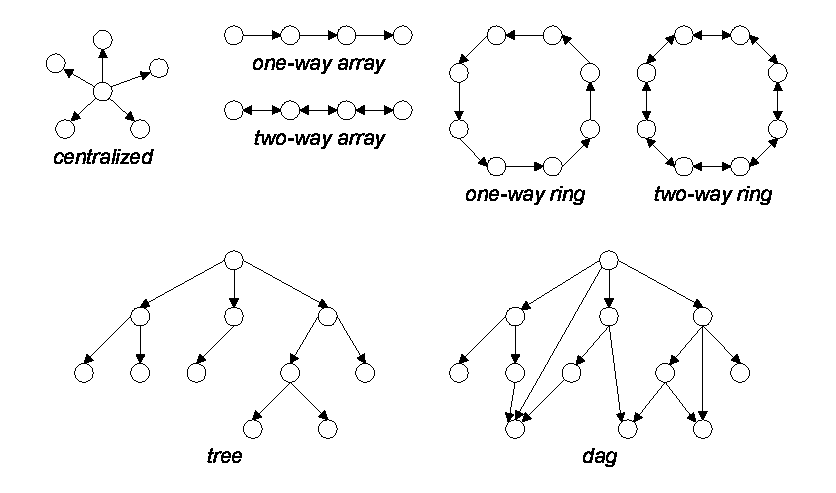
\includegraphics{img/pcgs/structur}
  \caption{Príklady komunikačných štruktúr $PCGS$} \label{pcgs_obr_structures}
\end{figure}

\begin{oznacenie}
$xPCGS_nX$ - trieda $PCGS$-systémov kde
$x\in\{centr,tree,dag,\dots\}$ je typ komunikačnej
štruktúry\footnote{ak nie je uvedený typ komunikačnej štruktúry,
máme na mysli triedu všetkých $PCGS$-systémov bez ohľadu na
štruktúru}, $n$ je počet komponentov ($(n=*)$ označuje ľubolný
počet komponentov) a $X\in\{REG,LIN,CF,\dots\}$ je typ
komponentov\footnote{lineárne gramatiky (LIN) sú bezkontextové
gramatiky, ktoré majú na pravej strane pravidiel najviac jeden
neterminál}.
\end{oznacenie}

\section{Generatívna sila $PCGS$}

Na bližšie pochopenie sily $PCGS$ si uvedieme najskôr zopár
príkladov.

\begin{priklad}
\label{pcgs_prikl_1}
$\Gamma_1=(\{S_1,S_2,S_3\},K,\{a,b,c\},G_1,G_2,G_3)$, kde množiny
pravidiel príslušných gramatík sú:
\begin{itemize}
  \item $P_1=\{S_1\ra aS_1,S_1\ra aQ_2,S_2\ra
  bQ_3,S_3\ra c\}$
  \item $P_2=\{S_2\ra bS_2\}$
  \item $P_3=\{S_3\ra cS_3\}$
\end{itemize}
Skúsme si napísať pár krokov odvodenia: \\ $(S_1,S_2,S_3)\Ra
(aS_1,bS_2,cS_3)\Ra\dots k-krokov\dots\Ra
(a^kS_1,b^kS_2,c^kS_3)\Ra\newline
(a^{k+1}Q_2,b^{k+1}S_2,c^{k+1}S_3)\Ra
(a^{k+1}b^{k+1}S_2,S_2,c^{k+1}S_3)\Ra
(a^{k+1}b^{k+2}Q_3,bS_2,c^{k+2}S_3)\Ra\newline
(a^{k+1}b^{k+2}c^{k+2}S_3,bS_2,S_3)\Ra
(a^{k+1}b^{k+2}c^{k+3},b^2S_2,cS_3)$ \\ Teraz už vidíme, že
$L(\Gamma_1)=\{a^nb^{n+1}c^{n+2}\mm n\geq 1\}$, a teda
centralizovaný $PCGS$ s troma re\-gu\-lárnymi komponentami
vygeneroval jazyk, ktorý nie je regulárny, ba dokonca ani
bezkontextový.
\end{priklad}

\begin{priklad}
\label{pcgs_prikl_2} $\Gamma_2=(\{S_1,S_2,A\},K,\{a,b,c\},G_1,G_2)$,
kde
\begin{itemize}
  \item $P_1=\{S_1\ra aS_1,S_1\ra Q_2,A\ra
  aS_1,A\ra c\}$
  \item $P_2=\{S_2\ra A,A\ra bA\}$
\end{itemize}
Napíšme si pár krokov odvodenia: \\ $(S_1,S_2)\Ra
(aS_1,A)\overset{*}\Ra (a^kS_1,b^{k-1}A)\Ra (a^k Q_2, b^k A)\Ra
(a^k b^k A, S_2)\Ra (a^k b^k aS_1,A)\Ra \dots$
\\ Ľahko vidno, že $L(\Gamma_2)=(\{a^nb^n\mm
n\geq 1\})^+c$, čo je opäť jazyk, ktorý nie je ani bezkontextový.
\end{priklad}

\begin{priklad}
\label{pcgs_prikl_3} $\Gamma_3=(\{S_1,S_2\},K,\{a,b,c,d\},G_1,G_2)$
\begin{itemize}
  \item $P_1=\{S_1\ra cS_1d,S_1\ra cQ_2d\}$
  \item $P_2=\{S_2\ra aS_2b,S_2\ra ab\}$
\end{itemize}
Všimnime si niektoré možné odvodenia:
\begin{enumerate}
  \item $(S_1,S_2)\overset{*}\Ra
  (c^{k-1}S_1d^{k-1},a^{k-1}S_2b^{k-1})\Ra (c^kQ_2d^k,a^kS_2b^k)\Ra
  (c^ka^kS_2b^kd^k,S_2)$ a tu sa $\Gamma_3$ zasekne
  \item $(S_1,S_2)\overset{*}\Ra
  (c^{k-1}S_1d^{k-1},a^{k-1}S_2b^{k-1})\Ra (c^kQ_2d^k,a^kb^k)\Ra
  (c^ka^kb^kd^k,S_2)$
  \item $(S_1,S_2)\overset{*}\Ra
  (c^{k-1}S_1d^{k-1},a^{k-1}S_2b^{k-1})\Ra
  (c^kS_1d^k,a^kb^k)\overset{*}\Ra
  (c^{k+i}Q_2d^{k+i},a^kb^k)\Ra\newline
  (c^{k+i}a^kb^kd^{k+i},a^kb^k)$
\end{enumerate}
Teda $L(\Gamma_3)=\{c^la^kb^kd^l\mm l\geq k\geq 1\}$. $PCGS$ s
dvoma lineárnymi komponentami vygeneroval jazyk mimo bezkontextovú
triedu jazykov.
\end{priklad}

\begin{priklad}
$\Gamma_4=(\{S_1,S_2\},K,\{a,b,c\},G_1,G_2)$
\begin{itemize}
  \item $P_1=\{S_1\ra S_1,S_1\ra Q_2cQ_2\}$
  \item $P_2=\{S_2\ra aS_2,S_2\ra bS_2,S_2\ra
  a,S_2\ra b\}$
\end{itemize}
Ľahko vidno, že $L(\Gamma_4)=\{wcw\mm w\in\{a,b\}^+\}$, a teda
$PCGS$ s dvoma bezkontextovými komponentami vygeneroval jazyk,
ktorý nie je bezkontextový.
\end{priklad}

\begin{priklad}
$\Gamma_5=(\{S_1,S_2,S_3\},K,\{a,b,c,d\},G_1,G_2,G_3)$
\begin{itemize}
  \item $P_1=\{S_1\ra aS_1,S_2\ra aQ_2,S_3\ra d\}$
  \item $P_2=\{S_2\ra bS_2,S_2\ra bQ_3\}$
  \item $P_3=\{S_3\ra cS_3\}$
\end{itemize}
Všimnime si odvodenie, v ktorom nasleduje po sebe viac
komunikačných krokov:
\\ $(S_1,S_2,S_3)\overset{*}\Ra (a^kS_1,b^kS_2,c^kS_3)\Ra
(a^{k+1}Q_2,b^{k+1}Q_3,c^{k+1}S_3)\Ra
(a^{k+1}Q_2,b^{k+1}c^{k+1}S_3,S_3)\Ra
(a^{k+1}b^{k+1}c^{k+1}S_3,S_2,S_3)\Ra
(a^{k+1}b^{k+1}c^{k+1}d,bS_2,cS_3)$ \\ Ľahko vidno, že
$L(\Gamma_5)=\{a^nb^nc^nd\mm n\geq 1\}\in
\mathcal{L}_{CS}-\mathcal{L}_{CF}$.
\end{priklad}

\begin{priklad}
V tomto príklade ukážeme ako $PCGS$ naplno využije silu svojej
komunikácie a vyrobíme jazyk $L(\Gamma)=\{ w^{2^n}c\mm w\in\{
a,b\}^*,n\geq 1\}$:
\\ $\Gamma_6=(\{ S_1,S_2,S_3\} ,K,\{ a,b\} ,G_1,G_2,G_3)$
\begin{itemize}
  \item $P_1=\{S_1\ra aS_1,S_1\ra bS_1,S_1\ra
  Q_2, \omega_1\ra Q_3,\omega_2\ra S_1',S_1'\ra c\}$
  \item $P_2=\{S_2\ra S_2,S_2\ra Q_1,S_1\ra\omega_1,
  S_1'\ra\omega_1\}$
  \item $P_3=\{S_3\ra S_3,S_3\ra Q_1,S_1\ra\omega_1,
  \omega_1\ra\omega_2,S_1'\ra\omega_1\}$
\end{itemize}
Pozrime sa na to ako funguje odvodenie v $\Gamma$:
\\ $(S_1,S_2,S_3)\overset{*}\Ra (wS_1,S_2,S_3)
\Ra (wS_1,Q_1,Q_1)\Ra (S_1,wS_1,wS_1)\Ra
(Q_2,w\omega_1,w\omega_1)\Ra\newline (w\omega_1,S_2,w\omega_1)\Ra
(wQ_3,S_2,w\omega_2)\Ra (ww\omega_2,S_2,S_3)\Ra
(wwS_1',Q_1,Q_1)\overset{*}\Ra (w^4S_1',Q_1,Q_1)\overset{*}\Ra
(w^{2^n}S_1',S_2,S_3)\Ra (w^{2^n}c,\dots )$
\\ Pravidlá v $\Gamma$ sú zostavené tak dômyselne, že gramatiky
$G_2$, $G_3$ naraz vygenerujú komunikačný symbol $Q_1$, teda
prenesú si vetnú formu vygenerovanú prvou gramatikou a následne
$G_1$ požiada o vetné formy $G_2$ a $G_3$, teda obsah vetnej formy
$G_1$ sa zdvojnásobí. Ak by gramatiky takto ``nespolupracovali'',
tak sa $\Gamma$ zasekne.
\\ Všimnime si ešte, že $\Gamma$ vygeneruje slovo $w^{2^n}c$ v
čase $O(n)$. $G_1$ na začiatku vygeneruje $w$ a potom pri každom
zdvojnásobení $\Gamma$ používa už len konštantný počet krokov
odvodenia. Treba si uvedomiť, že je to možné len vďaka tomu, že
pri modeli $PCGS$ máme komunikáciu v podstate zadarmo, lebo v
jednom kroku dokážeme preniesť ľubovoľne veľké slovo.
\end{priklad}

\begin{veta}
Niekoľko porovnaní $PCGS$ s triedami Chomského hierarchie:
\begin{enumerate}
  \item $\mathcal{L}(PCGS_nREG)-\mathcal{L_{LIN}}\neq\emptyset$ pre $n\geq 2$
  \item $\mathcal{L}(PCGS_nREG)-\mathcal{L_{CF}}\neq\emptyset$ pre $n\geq 3$
  \item $\mathcal{L}(PCGS_nLIN)-\mathcal{L_{CF}}\neq\emptyset$ pre $n\geq 2$
\end{enumerate}
\end{veta}

\begin{dokaz}
Pozri príklady \ref{pcgs_prikl_2}, \ref{pcgs_prikl_1} a \ref{pcgs_prikl_3}.
\end{dokaz}

\begin{veta}
\label{pcgs_veta_LLINtoLcentrPCGS*REG}
$\mathcal{L}_{LIN}-\mathcal{L}(centrPCGS_*REG)\neq\emptyset$
\end{veta}

\begin{dokaz}
Uvažujme jazyk $L=\{a^nb^mcb^ma^n\mm n,m\geq 1\}$. \\ Zrejme
$L\in\mathcal{L}_{LIN}$. Ukážeme, že
$L\not\in\mathcal{L}(centrPCGS_*REG)$. \\ Bez ujmy na všeobecnosti
môžme predpokladať, že $G_1$ negeneruje $a$-čka, lebo ak by
generovala tak to isté dokáže aj iný komponent a $G_1$ môže
požiadať o jej výstup. Teda $a$-čka generujú dve iné gramatiky
($G_2,G_3$), lebo potrebujeme rovnaký počet $a$-čiek na začiatku
aj na konci vetnej formy. Podobne musia existovať aj dve gramatiky
($G_4,G_5$) na generovanie $b$-čiek. Ak po nejakom počte krokov
$G_1$ vygeneruje $Q_2$, tak v konečnom (dosť malom) počte krokov
musí vygenerovať aj $Q_3$, lebo $G_3$ sa nemá ako dozvedieť, že už
nemá generovať $a$-čka, keďže uvažujeme centralizovanú komunikačnú
štruktúru. Z toho ale plynie, že v tomto konečnom počte krokov
musí $G_1$ vygenerovať $Q_4$ a $Q_5$, lebo uvažujeme regulárne
gramatiky. Teda $G_4$ a $G_5$ majú obmedzený čas na generovanie
$b$-čiek, a teda počet $b$-čiek nemôže byť oveľa
väčší\footnote{$m$ môže byť väčšie od $n$ najviac lineárne v
závislosti od pravidiel v $G_2,G_3$ a v $G_4,G_5$} ako počet
$a$-čiek, čo je spor s tým, že potrebujeme vygenerovať aj slová s
ľubovoľne veľkým rozdielom medzi $m$ a $n$.
\end{dokaz}

\pagebreak

\begin{veta}
$\mathcal{L}(centrPCGS_2REG)\subsetneq\mathcal{L}_{CF}$
\end{veta}

\begin{dokaz}
Podľa vety \ref{pcgs_veta_LLINtoLcentrPCGS*REG} stačí dokázať už len
inklúziu $\subseteq$:
\\ Majme $\Gamma=(N,K,T,G_1,G_2)\in centrPCGS_2REG$. Chceme
zostrojiť bezkontextovú gramatiku $G=(N',T,P,S)$ takú, že
$L(\Gamma)=L(G)$. Rozšírime množinu neterminálov takto:\\
$N'=N\cup \{[A,B]\mm A\in N,B\in N\}\cup\{\overline{A}\mm A\in
N\}$, neskôr si ukážeme ako tieto nové neterminály budeme
využívať. Najskôr sa zamyslime nad tým, ako bude vyzerať výsledné
slovo $w\in L(\Gamma)$.\linebreak $w$ bude mať nasledujúce
vlastnosti (obr.\ref{pcgs_obr_l2reglcf}):

\begin{enumerate}
  \item $w$ sa dá dekomponovať na $w=w_1w_2\dots w_s$ pre nejaké $s\geq 1$
  \item $\forall i\; w_i=v_{i_1}v_{i_2}$ pričom $v_{i_1}$ generuje $G_1$
  a $v_{i_2}$ generuje $G_2$
  \item $v_{i_1}$ a $v_{i_2}$ sú generované na rovnaký počet
  krokov
\end{enumerate}

\begin{figure}[ht]
  \centering
  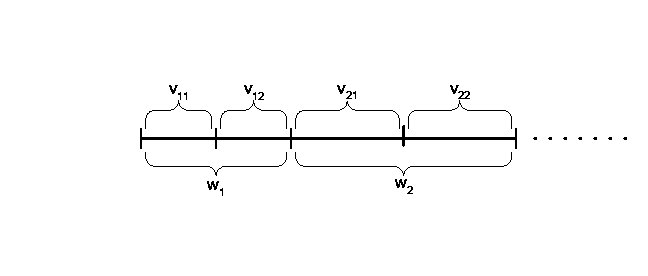
\includegraphics{img/pcgs/l2reglcf}
  \caption{Tvar slova generovaného $centrPCGS_2REG$}\label{pcgs_obr_l2reglcf}
\end{figure}

$G$ musí byť schopná generovať slová s takýmito vlastnosťami. Na
zabezpečenie podmienky 3 bude $G$ generovať jednotlivé podslová
$w_i$ odstredu t.j. nejaký špeciálny neterminál sa bude postupne
obklopovať terminálmi podľa pravidiel $G_1,G_2$.
\\ V $P$ budú pravidlá:
\begin{description}
  \item{$S\ra [S_1,B] B$  $\forall B\in N$} \\Teda máme špeciálnu
  sadu neterminálov $[S_1,B]$, ktoré určujú, že podslovo $v_{1_1}$
  sa začína generovať z počiatočného neterminálu $S_1$ a podslovo
  $v_{1_2}$ bude mať posledný neterminál $B$. To v podstate znamená,
  že $G$ sa nedeterministicky rozhodne pre neterminál $B$.
  \item{$[A,B]\ra a[A',B']b$  ak $A\ra aA'\in P_1$ a $B'\ra bB\in
  P_2$} \\ Tieto pravidlá nám zabezpečujú postupné simulovanie
  odvodenia slov $v_{i_1}$ odpredu a slov $v_{i_2}$ odzadu, pričom
  toto odvodenie bude legálne vzhľadom na pravidlá $G_1,G_2$.
  \item{$[Q_2,S_2]\ra\varepsilon$} \\ Toto pravidlo zabezpečuje, že
  ak $G$ na začiatku dobre uhádla posledný neterminál $v_{i_2}$, tak
  po konečnom počte krokov simulácia $G_1$ dospela ku komunikačnému
  neterminálu $Q_2$ a simulácia $G_2$ v spätnom odvodení dospela k
  počiatočnému neterminálu $S_2$, teda neterminál $[Q_2,S_2]$ sa už
  nebude ďalej rozvíjať, a teda ho vymažeme.
  \item{$A\ra [A,B]B$  $\forall A,B\in N$} \\ Tieto pravidlá slúžia na
  správne nadväzovanie podslov $w_i$, $w_{i+1}$. To znamená, že
  týmto pravidlom $G$ uhádne akým neterminálom bude končiť ďalšie
  podslovo.
\end{description}
Ukážme si teraz ako funguje simulácia. Zoberme si nejaké odvodenie
v $\Gamma$.
\\ $(S_1,S_2)\Ra (u_1A_1,v_1B_1)\overset{*}\Ra (u_1u_2\dots u_kQ_2,v_1v_2\dots
v_kB_k)\Ra (u_1\dots u_kv_1\dots v_kB_k,S_2)\Ra\dots$
\\ Príslušná časť odvodenia v $G$ bude vyzerať takto:
\\ $S\Ra [S_1,B_k]B_k\Ra u_1[A_1,B_{k-1}]v_kB_k\Ra u_1u_2[A_2,B_{k-2}]v_{k-1}v_kB_k
\overset{*}\Ra\newline u_1\dots u_k[Q_2,S_2]v_1\dots v_kB_k\Ra
u_1\dots u_kv_1\dots v_kB_k\Ra\dots$
\\ $G$ najskôr nedeterministicky vybrala pravidlo $S\ra
[S_1,B_k]B_k$ tak, aby správne uhádla neterminál, ktorým bude
ďalej pokračovať $G_1$ v odvodení po komunikačnom kroku (t.j.
neterminál, ktorý bol prenášaný v komunikačnom kroku). Potom
postupne simulovala odvodenie $G_1$, $G_2$ a nakoniec vymazala
neterminál $[Q_2,S_2]$ z vetnej formy. Takto ostal vo vetnej forme
len neterminál $B_k$, ktorým začne ďalšiu simuláciu $G_1$. Teraz
$G$ použije nejaké z pravidiel $B_k\ra [B_k,B]B$ na uhádnutie
neterminálu, ktorý bude prenášaný v nasledujúcom komunikačnom
kroku atď.

\smallskip

Ešte sa musíme zamyslieť nad tým, ako simuláciu ukončiť. Môžu
nastať dva prípady:
\begin{enumerate}
  \item $G_1$ už nepožiada $G_2$ o jej vetnú formu (teda nevyprodukuje $Q_2$)
  a sama vyprodukuje terminálne slovo. Pre túto možnosť dodáme do
  $P$ tieto pravidlá:
  \begin{itemize}
    \item $B\ra \overline{B}$  $\forall B\in N$
    \item $\overline{A}\ra u\overline{B}$ ak $A\ra uB\in P_1$
  \end{itemize}
  Tým, že sme použili ``pruhované'' neterminály a nemáme pravidlo
  typu $\overline{A}\ra A$ sme zmarili ďalšiu\footnote{k dispozícii
  máme samozrejme aj pravidlo $S\ra\overline{S}$ teda
  žiadna komunikácia nemusí nastať} komunikáciu, a teda simulujeme
  $G_1$ až kým nevygeneruje terminálne slovo.
  \item $G_2$ skončí skôr (t.j. vygeneruje terminálne slovo) ako
  $G_1$ požiada o jej vetnú formu. V $\Gamma$ sa vetná forma $G_2$
  nemení a čaká, kým $G_1$ vygeneruje $Q_2$. Pre túto možnosť dodáme
  do $P$ tieto pravidlá:
  \begin{itemize}
    \item $A\ra [A,\varepsilon]$  $\forall A\in N$
    \item $[A,\varepsilon]\ra u[A',\varepsilon]$ ak $A\ra uA'\in P_1$
    \item $[A,\varepsilon]\ra u[A',B]$  $\forall B\in N$ ak $A\ra uA'\in P_1$
  \end{itemize}
Teda pravidlá typu $[A,\varepsilon]\ra u[A',\varepsilon]$ simulujú
čakaknie $G_2$ na komunikáciu a pravidlá typu $[A,\varepsilon]\ra
u[A',B]$ opäť slúžia na uhádnutie posledného neterminálu, ktorý sa
objavil vo vetnej forme $G_2$.
\end{enumerate}
\end{dokaz}

\begin{lema}
\label{pcgs_lema_pumplemacentrPCGSnREG} (Pumpovacia lema pre
$centrPCGS_nREG$)
\\ Nech $L\in\mathcal{L}(centrPCGS_nREG)$. Potom existuje prirodzené číslo $M$, že
$\forall w\in L$ také, že\linebreak $|w|>M$ existuje $m$ $1\leq
m\leq n$ a existujú $x_i,y_i$ tak, že sú splnené nasledovné
podmienky:
\begin{enumerate}
  \item $w=x_1y_1x_2y_2\dots x_my_mx_{m+1}$
  \item $\forall i$ $y_i\neq\varepsilon$
  \item $\forall k\geq 0\; :\; x_1{y_1}^kx_2{y_2}^k\dots x_m{y_m}^kx_{m+1}\in L$
\end{enumerate}
\end{lema}

\begin{dokaz}
Nech $\Gamma=(N,K,T,G_1,\dots ,G_n)\in centrPCGS_nREG$. Každá
gramatika má vo svojej vetnej forme najviac jeden neterminál a ten
je posledným symbolom tejto vetnej formy. Teda konfigurácia
$\Gamma$ je tvaru $c=(x_1A_1,x_2A_2,\dots ,x_nA_n)$. Budeme
hovoriť, že dve konfigurácie $c_1=(x_1A_1,x_2A_2,\dots ,x_nA_n)$ a
$c_2=(y_1B_1,y_2B_2,\dots ,y_nB_n)$, kde $\forall i\; x_i,y_i\in
T^+$ a $\forall i\; A_i,B_i\in N\cup\{\varepsilon\}$ sú
ekvivalentné (ozn. $c_1\equiv c_2$), ak $\forall i :\; A_i=B_i$.
\\ Uvažujme slovo $w\in L(\Gamma)$ a jeho odvodenie minimálnej
dĺžky. Ak $M$ je počet všetkých možných rôznych výskytov
neterminálov vo vetných formách\footnote{tých je $M=|N\cup K|^n$},
tak za predpokladu, že $|w|>M$, existujú v tomto odvodení dve
konfigurácie $c_1$ a $c_2$ spĺňajúce nasledovné podmienky:
\begin{enumerate}
  \item $c_1\equiv c_2$
  \item ak je v odvodení medzi konfiguráciami $c_1$ a $c_2$ použitý
  komunikačný symbol $Q_i,\; 2\leq i\leq n$, tak $x_i=y_i$
\end{enumerate}
Teda odvodenie je tvaru: \\ $(S_1,S_2,\dots ,S_n)\overset{*}\Ra
(x_1A_1,x_2A_2,\dots ,x_nA_n)\overset{*}\Ra
(x_1z_1A_1,x_2z_2A_2,\dots ,x_nz_nA_n)\overset{*}\Ra (w,\dots)$ \\
Ak je v odvodení medzi konfiguráciami $c_1$ a $c_2$ použitý
komunikačný symbol $Q_i,\; 2\leq i\leq n$, tak podľa podmienky (2)
platí, že $z_i=\varepsilon$. Pre ostatné komponenty konfigurácie
nastáva jedna z nasledujúcich možností:
\begin{enumerate}
  \item $z_1\in T^+$ t.j. $z_1$ je neprázdne terminálne slovo.
  \item existuje $j,\; 2\leq j\leq n$ také, že $Q_j$ nie je použité v odvodení medzi
  konfiguráciami $c_1$ a $c_2$ ale je použité v odvodení, ktoré
  začína konfiguráciou $c_2$, naviac $z_j\in T^+$ teda $z_j$ je
  neprázdne terminálne slovo.
\end{enumerate}
Predpokladajme, že ani jedna z týchto možností nenastane. Potom
jednotlivé komponenty konfigurácií $c_1$ a $c_2$ sú totožné. Z
toho vyplýva, že časť odvodenia ($c_1\overset{*}\Ra c_2$) medzi
konfiguráciami $c_1$ a $c_2$ môžeme z odvodenia vynechať, čím
dostaneme kratšie odvodenie slova $w$, čo je spor s predpokladom,
že sme uvažovali najkratšie odvodenie $w$. \\ Teda jedna z
uvedených možností určite nastane. V tomto prípade môžeme
postupnosť krokov odvodenia medzi $c_1$ a $c_2$ opakovať $k$ krát
pre ľubovoľné\footnote{ak túto postupnosť krokov úplne vynecháme,
tiež dostaneme legálne odvodnie v $\Gamma$, teda pripúšťame aj
$k=0$ } $k$. Po týchto $k$ iteráciach sa komponent $j$, pre ktorý
$z_j$ bolo neprázdne terminálne slovo, zmení na $x_j{z_j}^kA_j$.
Ak po týchto $k$ ite\-rá\-ciach dokončíme odvodenie časťou pôvodného
odvodenia $c_2\overset{*}\Ra (w,\dots )$, tak dostaneme nové slovo
$w'\in L(\Gamma)$, ktoré sa od pôvodného $w$ líši napumpovaním
časti $z_j$. \\ Ak si uvedomíme, že počet podslov, ktoré môžu byť
takto pumpované, môže byť najviac $n$, tak sme s dôkazom tejto
lemy hotoví.
\end{dokaz}

\smallskip

Podobné pumpovacie lemy platia aj pre triedy $treePCGS_nREG$
a $dagPCGS_nREG$, avšak pre všeobecnú necentralizovanú
komunikačnú štruktúru $PCGS$ sa pumpovať nedá.

\begin{veta}
$\mathcal{L}(centrPCGS_{n-1}REG)\subsetneq\mathcal{L}(centrPCGS_nREG)$
pre $n\geq 2$
\end{veta}

\begin{dokaz}
Inklúzia $\subseteq$ je zrejmá.
\\ Treba ukázať, že existuje jazyk
$L$ taký, že $L\in\mathcal{L}(centrPCGS_nREG)$ a\newline
$L\not\in\mathcal{L}(centrPCGS_{n-1}REG)$. Uvažujme jazyky $L_n=\{
{a_1}^{k+1}{a_2}^{k+2}{a_3}^{k+3}\dots {a_n}^{k+n}\mm k\geq 0\}$.
Zostrojme $centrPCGS_nREG$ $\Gamma_n=(\{S_1,\dots
,S_n\},K,\{a_1,\dots ,a_n\},G_1,\dots ,G_n)$, kde
\begin{itemize}
  \item $P_1=\{S_1\ra a_1S_1,S_n\ra a_n\}\cup\{ S_i\ra a_iQ_{i+1}\mm 1\leq
  i\leq n-1\}$
  \item $P_j=\{S_j\ra a_jS_j\}$ pre $2\leq j\leq n$
\end{itemize}
Zrejme\footnote{čitateľovi
 to môže byť zrejmejšie, ak sa pozrie na príklad \ref{pcgs_prikl_1}}
$L(\Gamma_n)=L_n$. Chceme ukázať, že
$L_n\not\in\mathcal{L}(centrPCGS_{n-1}REG)$. Sporom,
predpokladjme, že $L_n\in\mathcal{L}(centrPCGS_{n-1}REG)$. Podľa
lemy \ref{pcgs_lema_pumplemacentrPCGSnREG} pre tento jazyk existuje
prirodzené číslo $M$. Zoberme si slovo
$w={a_1}^{M+1}{a_2}^{M+2}{a_3}^{M+3}\dots {a_n}^{M+n}\in L_n$.
Zjavne $|w|\geq M$. Slovo $w$ môžme pumpovať najviac na $n-1$
miestach. Aby toto slovo po pumpovaní ostalo v $L_n$ potrebujeme
ho pumpovať na $n$ miestach, a to je spor s predpokladom.
\end{dokaz}

\begin{dosledok}
Hierarchia $\mathcal{L}(centrPCGS_nREG),\; n\geq 1$ je nekonečná.
\end{dosledok}

Podobnými dokazovacími technikami (t.j. využitím pumpovacích liem
pre nejaký jazyk) by sme sa dopracovali k nasledujúcim dvom
tvrdeniam:

\begin{veta}
Hierarchie nasledujúcich tried sú nekonečné:
\begin{itemize}
\item $\mathcal{L}(treePCGS_nREG),\; n\geq 1$
\item $\mathcal{L}(dagPCGS_nREG),\; n\geq 1$
\end{itemize}
\end{veta}


Hoci pre triedy $PCGS$ s komunikačnými štruktúrami $array$ a
$ring$ nie sú známe pumpovacie lemy, inými spôsobmi sa dájú
dokázať nasledujúce tri tvrdenia:

\begin{veta}
Hierarchie nasledujúcich tried sú nekonečné:
\begin{itemize}
\item $\mathcal{L}(two-way-arrayPCGS_nREG),\; n\geq 1$
\item $\mathcal{L}(two-way-ringPCGS_nREG),\; n\geq 1$
\item $\mathcal{L}(one-way-ringPCGS_nREG),\; n\geq 1$
\end{itemize}
\end{veta}

\begin{veta}
$\mathcal{L}(PCGS_{n-1}REG)\subsetneq\mathcal{L}(PCGS_nREG)$ pre
$n\geq 2$
\end{veta}

\begin{dokaz}
Uvažujme jazyky $L_n=\{{a_1}^k{a_2}^k\dots a^k_{2n-2}\mm k\geq
1\}$. Dá sa skonštruovať \newline $\Gamma\in PCGS_nREG$ tak, že
$L(\Gamma)=L_n$. Potom zrejme $L_n\in\mathcal{L}(PCGS_nREG)$.
Treba ukázať, že $L_n\not\in\mathcal{L}(PCGS_{n-1}REG)$. Tento
dôkaz je však dosť technický, a preto ho tu nebudeme
uvádzať\footnote{podrobnosti možno nájsť v \cite{impact}}.
\end{dokaz}

\begin{dosledok}
Hierarchia $\mathcal{L}(PCGS_nREG),\; n\geq 1$ je nekonečná.
\end{dosledok}

\begin{poznamka}
Otvorenými problémami zostávajú nekonečnosť hierarchií\newline
$\mathcal{L}(centrPCGS_nX),\mathcal{L}(PCGS_nX)$ pre $n\geq 1$ a
$X\in\{ CF,CS\}$.
\end{poznamka}

\section{Porovnanie $PCGS$ so sekvenčnými triedami}

\begin{veta}
\label{pcgs_veta_multicounter} Nech $\Gamma$ je $treePCGS_mREG(f(n))$,
kde $f(n)$ je počet komunikačných krokov potrebných na
vygenerovanie slova dĺžky $n$. Potom existuje\footnote{n
počítadlový automat je zásobníkový automat s n zásobníkmi, ktoré
pracujú nad jednopísmenkovou abecedou} nedeterministický ($m-1$)
počítadlový automat $M$ pracujúci v lineárnom čase a akceptujúci
jazyk $L(\Gamma)$ pričom vykoná $2f(n)$ obratov\footnote{zmena
smeru hlavy v zásobníku resp. zmena inkrementácie counteru na
dekrementáciu a opačne} a $f(n)$ testov na
nulu\footnote{dosiahnutie dna zásobníka resp. counter dosiahol
nulu}.
\end{veta}

\pagebreak

\begin{dokaz}
Nech $\Gamma$ má komponenty $G_1,\dots ,G_m$. Chceme zostrojiť
nedeterministický ($m-1$) počítadlový automat $M$ simulujúci
$\Gamma$. Celá simulácia $\Gamma$ nám bude jasnejšia, ak sa
zamyslíme nad tým, ako môže vyzerať slovo $w\in L(\Gamma)$ pri
stromovej komunikačnej štruktúre. Slovo $w=w_{i_1}w_{i_2}\dots
w_{i_k}$, $\forall j\; i_j\in\{1,\dots ,m\}$ pozostáva z podslov
$w_{i_j}$ generovaných gramatikami $G_i$, pričom dĺžky týchto
podslov závisia od konkrétnej komunikačnej štruktúry
(obr.\ref{pcgs_obr_pocitad}).

\begin{figure}[ht]
  \centering
  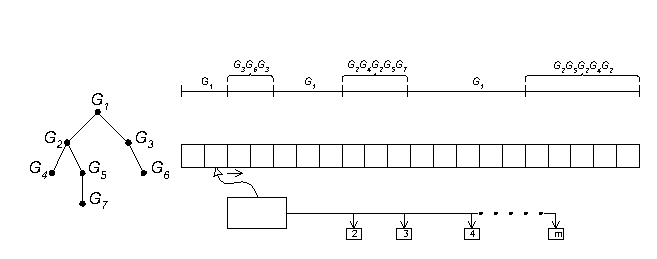
\includegraphics{img/pcgs/pocitad}
  \caption{Viacpočítadlový automat a tvar slova generovaného $treePCGS$}\label{pcgs_obr_pocitad}
\end{figure}

Vieme, že každá regulárna gramatika sa dá simulovať pomocou
nedeterministického konečného automatu\footnote{pozri
\cite{Hopc}}. Podobne budú v pravidlách nášho automatu $M$
simulované pravidlá regulárnych komponentov $G_1,\dots ,G_m$. $M$
bude používať svoje počítadlá $C_2,\dots ,C_m$ na zabepečenie
toho, aby jednotlivé gramatiky $G_1,\dots ,G_m$ neboli simulované
dlhšie ako to vyžaduje daná situácia (konfigurácia). V každej
konfigurácii $M$ bude číslo $c(C_i)\; \forall i\in\{2,\dots ,m\}$
uložené v $C_i$ uchovávať rozdiel medzi počtom prepisovacích
krokov $G_i$ simulovaných $M$ a počtom prepisovacích krokov otca
$G_i$ v stromovej komunikačnej štruktúre (to znamená, že ak $G_i$
je požiadaná svojim otcom o vyprodukovanú vetnú formu, tak túto
vetnú formu môže $G_i$ generovať najviac $c(C_i)$ krokov).
\\ $M$ nedeterministicky striedavo simuluje gramatiky $G_1,\dots ,G_m$ a
zároveň overuje, či slovo ge\-ne\-ro\-va\-né gramatikami je zhodné
so slovom na vstupnej páske. Na začiatku $M$ simuluje $G_1$ a
priebežne overuje vstupnú pásku. Zároveň po každom odsimulovanom
prepisovacom kroku $G_1$ inkrementuje počítadlá všetkým synom
$G_1$ a ostatné počítadlá zostanú nezmenené. Simulácia $G_1$
skončí, keď $G_1$ vygeneruje komunikačný symbol $Q_i$ pre nejaké
$i$. $M$ začne simulovať gramatiku $G_i$ z počiatočného
neterminálu $S_i$. Počas tejto simulácie po každom prepisovacom
kroku $G_i$ sa dekrementuje počítadlo $C_i$ a inkrementujú sa
počítadlá všetkých sy\-nov $G_i$. Ak $G_i$ vyprodukuje terminálnu
vetnú formu, tak $M$ zastaví a akceptuje vstupné slovo práve
vtedy, keď bol vstup prečítaný až do konca. Ak $C_i$ je prázdne
($c(C_i)=0$) a $G_i$ v poslednom kroku vygeneroval na konci
neterminál $A$, tak $M$ začne simulovať otca $G_i$ (v tomto
prípade $G_1$) pričom pokračuje v prepisovaní z neterminálu $A$.
Ak $G_1$ nemôže prepísať $A$ (t.j. nemá pravidlá na $A$), tak $M$
neakceptuje vstupné slovo. Ak $G_i$ vegeneruje komunikačný symbol
$Q_j$ pre nejaké $j$, tak $M$ začne simulovať $G_j$ (kde $G_j$ je
synom $G_i$) z počiatočného neterminálu $S_j$. $M$ od tohto
momentu po každom prepisovacom kroku $G_j$ dekrementuje $C_j$ a
inkrementuje počítadlá všetkých svojich synov. $M$ takto
rekurzívne simuluje gramatiky až kým poslená gramatika
nevygeneruje terminálnu vetnú formu. \\ Z popisu práce $M$ by malo
by zrejmé, že počet obratov je $2f(n)$ a počet testov na nulu je
$f(n)$, lebo počítadlo $C_i$ začne klesať práve vtedy, keď je
vygenerovaný komunikačný symbol $Q_i$. \\ Ak sa v pravidlách
gramatík nenachádzajú žiadne $chain rules$\footnote{pravidlá typu
$A\ra B$ kde $A,B$ sú neterminály}, tak $M$ pracuje v čase $n$. Ak
sú v gramatikách takéto pravidlá, tak $M$ pracuje v čase $O(n)$,
pretože existuje konštanta $d$ taká, že pre každé $w\in L(\Gamma)$
existuje odvodenie, ktoré v každých $d$ krokoch vygeneruje aspoň
jeden terminál.
\end{dokaz}

\medskip

Uvedomme si, že $m-1$ počítadlový automat vieme simulovať
viacpáskovým TS pracujúcim v rovnakom čase, a že počítadlá
uchovávajú čísla veľkosti najviac $n$,takže v binárnom kódovaní sa
zmestia do priestoru $O(\log n)$ Z týchto dvoch poznatkov plynie
nasledujúce tvrdenie.

\begin{veta}
$\mathcal{L}(treePCGS_mREG(f(n))\subseteq NTIME(n)\cap NSPACE(\log
n)$
\end{veta}

\begin{poznamka}
Predchádzajúca veta nehovorí, že vieme zostrojiť ekvivalentný TS
pracujúci v lineárnom čase a logaritmickom priestore. Hovorí len,
že vieme zostrojiť ekvivalentný TS pracujúci v lineárnom čase a
(iný) ekvivalentný TS pracujúci v logaritmickom priestore.
\end{poznamka}

Skúsme sa zamyslieť nad simuláciou $PCGS_mREG(f(n))$ priamočiaro
pomocou $m$-páskového TS. Ten by na každej páske simuloval
prepisovanie vetnej formy jednej gramatiky. Komunikácia medzi
gramatikami v tomto prípade znamená presunutie obsahu jednej pásky
na druhú. Keďže veľkosť pásky je $O(n)$ a komunikácií je $f(n)\in
O(n)$, tak časová zložitosť je $O(n^2)$. Pri takejto simulácii sa
nám ľahko môže stať, že nejaký kúsok vetnej formy bol presúvaný
medzi páskami $O(n)$ krát a nakoniec sa aj tak nedostal do
výsledného terminálneho slova. V nasledujúcej vete budeme toto
``zbytočné'' presúvanie eliminovať a dostaneme dobrý výsledok pre
$dagPCGS$.

\begin{veta}
$\mathcal{L}(dagPCGS_*REG)\subseteq NTIME(n)$
\end{veta}

\begin{dokaz}
Nech $\Gamma=(N,K,T,G_1,\dots ,G_m)\in dagPCGS_mREG$. Chceme
zostrojiť $m$-páskový\footnote{to znamená, že TS $A$ má $m$ hláv}
nedeterministický TS $A$ pracujúci v lineárnom čase a akceptujúci
jazyk $L(\Gamma)$.
\\ V $\delta$-funkcii si $A$ uchováva pravidlá všetkých m gramatík
a v stavoch si drží aktuálne neterminály\footnote{keďže gramatiky
sú regulárne, vo vetnej forme danej gramatiky sa vyskytuje najviac
jeden neterminál} všetkých gramatík. Na páskach $T_1,\dots ,T_m$
sú vetné formy generované gramatikami $G_1,\dots ,G_m$ alebo $T_i$
obsahuje blank symbol $B$, ak sa $A$ nedeterministicky rozhodne,
že vetnú formu, ktorú generuje $G_i$ sa neobjaví vo výslednom
terminálnom slove generovanom $\Gamma$ t.j eliminovanie
\mbox{``zbytočných''} presúvaní z jednej pásky na druhú.
\\ Na začiatku bude $A$ v stave so začiatočným neterminálom pre
každú gramatiku. Pre každé $i=1..m$ $A$ uhádne, či sa vetná forma
generovaná gramatikou $G_i$ bude nachádzať vo výslednom
terminálnom slove. Ak $A$ rozhodne, že vetná forma generovaná
$G_i$ bude vo výslednom slove, tak $A$ bude simulovať odvodenie
gramatiky $G_i$ na páske $T_i$. Ak $A$ rozhodne, že nebude, tak
$A$ zapíše na pásku $T_i$ symbol $B$ a ďalej nesimuluje odvodenie
$G_i$ na páske $T_i$. Takto $A$ simuluje iba to, čo sa vo
výslednom slove naozaj objaví.
\\ Jeden krok simulácie $A$ pozostáva z jedného prepisovacieho kroku
každej z gramatík, pre ktoré sa $A$ rozhodol, že ich bude
simulovať. To môžeme, lebo ako sme si povedali $A$ si v stave
uchováva aktuálne neterminály každej z gramatík. Takto $A$
pokračuje, až kým sa na páske $T_1$ neobjaví terminálne slovo,
alebo až kým sa aspoň na jednej páske neobjaví $query$ symbol. \\
Ak sa na $T_1$ objaví terminálne slovo, tak $A$ porovná obsah
pásky $T_1$ so vstupom a ak sa rovnajú, tak $A$ akceptuje vstupné
slovo.

Ak aktuálny neterminál $G_i$ je $Q_j$ a
\begin{itemize}
  \item ani $T_i$ ani $T_j$ neobsahuje $B$, tak $A$ prekopíruje obsah
  $T_j$ na miesto $Q_j$ na páske $T_i$ a celý obsah pásky $T_j$
  prepíše na $S_j$ (počiatočný neterminál gramatiky $G_j$). Po tomto
  pokračuje $A$ v simulácii $G_i$ z neterminálu, ktorý bol posledným
  symbolom pri kopírovaní. $A$ uhádne, či ďalšia vetná forma
  generovaná $G_j$ bude časťou výsledného slova alebo nie. Podľa
  toho začne simulovať $G_j$ z počiatočného neterminálu $S_j$ alebo
  na $T_j$ zapíše $B$.
  \item buď $T_i$ alebo $T_j$
  obsahuje $B$, tak to znamená, že $A$ uhádol nesprávne\footnote{Ak
  $T_j$ obsahuje $B$, tak $T_i$ sa objaví vo výsledku, a teda aj
  $T_j$ bude vo výsledku, keďže si ju $G_i$ vyžiadala, teda $A$ zle
  uhádol. Ak $T_i$ obsahuje $B$, tak $T_j$ sa má objaviť vo
  výsledku, ale nemá sa ako dostať cez $T_i$, takže $A$ zle uhádol.} a
  výpočet sa zasekne.
  \item $T_i$ aj $T_j$ obsahuje $B$, tak $A$ nezmení obsah $T_i$ a
  nedeterministicky uhádne, či sa ďalšia vetná forma generovaná
  $G_j$ objaví vo výslednom terminálnom slove. Podľa toho $A$ začne na
  $T_j$ simulovať $G_j$ od počiatočného neterminálu $S_j$ alebo na
  $T_j$ nechá $B$.
\end{itemize}
Ak sa naraz na viacerých páskach objavia komunikačné symboly, tak
$A$ kopíruje vetné formy v určitom poradí tak, aby nekopíroval
nejaký komunikačný symbol. To sa určite dá, pretože uvažujeme
komunikačnú štruktúru $dag$, ktorá nepripúšťa cykly. \\ Pre každé
slovo $w\in L(\Gamma)$ existuje postupnosť správnych
nedeterministických rozhodnutí TS $A$, ktorá vedie k odvodeniu
tohto slova na páske $T_1$. Keďže komunikačná štruktúra nepripúšťa
cykly, tak každý symbol akceptovaného slova $w$ bol kopírovaný z
jednej pásky na druhú najviac $m-1$ krát, čo je konštantne veľa.
Teda na prekopírovanie všetkých symbolov slova $w$ potrebujeme čas
$O(n)$. Na páskach generujeme iba symboly, ktoré sa objavia vo
výslednom slove $w$, teda na vygenerovanie všetkých symbolov slova
$w$ potrebujeme čas $O(n)$. Konečne na porovnanie terminálneho
slova na páske $T_1$ so vstupom potrebujeme čas $O(n)$. Teda
celkovo pracuje $A$ v čase $O(n)$.
\end{dokaz}

\medskip

Uvedieme ešte niekoľko tvrdení, ktoré hovoria o tom, že ani
zvýšenie počtu gramatík, ani zvýšenie počtu komunikačných liniek v
stromovej štruktúre nedokáže vykompenzovať obmedzenie počtu
komunikačných krokov.

\begin{veta}
$\mathcal{L}(centrPCGS_2REG(n))-\mathcal{L}(treePCGS_*REG(f(n)))\neq\emptyset$
pre $f(n)\not\in\Omega (n)$
\end{veta}

\begin{dokaz}
Uvedieme\footnote{podrobnosti možno nájsť v \cite{some}} len, že
dôkaz uvažuje jazyk \newline \centerline{$L=\{
a^{i_1}b^{i_1}a^{i_2}b^{i_2}\dots a^{i_k}b^{i_k}c\mm k\geq 1,
i_j\geq 1\; pre\; j\in\{ 1,\dots ,n\}\}$} o ktorom sa ukáže, že
$L\in \mathcal{L}(centrPCGS_2REG(n))$ a
$L\not\in\mathcal{L}(treePCGS_*REG(f(n)))$. Využíva sa pri tom
simulácia $treePCGS_mREG(f(n))$ pomocou $m-1$ počítadlového
automatu ako to bolo uvedené vo vete \ref{pcgs_veta_multicounter}.
\end{dokaz}

\begin{veta}
Pre $f(n)\not\in\Omega (n)$ platí:
\begin{itemize}
  \item $\mathcal{L}(one-way-arrayPCGS_m(f(n)))\subsetneq\mathcal{L}(one-way-arrayPCGS_m(n))$
  pre $m\geq 2$
  \item $\mathcal{L}(centrPCGS_m(f(n)))\subsetneq\mathcal{L}(centrPCGS_m(n))$
  pre $m\geq 2$
  \item $\mathcal{L}(treePCGS_m(f(n)))\subsetneq\mathcal{L}(treePCGS_m(n))$
  pre $m\geq 2$
\end{itemize}
\end{veta}

\begin{veta}
$\mathcal{L}(centrPCGS_{k+1}(k))-\mathcal{L}(treePCGS_*(k-1))\neq\emptyset$
pre ľubovoľnú konštantu $k$.
\end{veta}

\begin{veta}
Pre ľubovoľné $k\geq 1$ a ľubovoľné
$x\in\{centr,tree,one-way-array\}$ platí:
\begin{itemize}
  \item $\mathcal{L}(xPCGS_{k+1}(k-1))\subsetneq\mathcal{L}(xPCGS_{k+1}(k))$
  \item $\mathcal{L}(xPCGS_*(k-1))\subsetneq\mathcal{L}(xPCGS_*(k))$
\end{itemize}
\end{veta}

\section{Niektoré ďalšie vlastnosti $PCGS$}

\begin{veta}
$\mathcal{L}(PCGS_*CF)$ je úplná $AFL$.
\end{veta}

\begin{veta}
$centrPCGS_*CF {<_4}^{Var} CF$
\end{veta}

\begin{veta}
$centrPCGS_*CF {<_4}^{Prod} CF$
\end{veta}

\section{Porovnanie $PCGS$ s $g$-systémami}

\begin{veta}
  Pre každý $PCGS_mREG$ $\Gamma$ existuje $g$-systém $G$ taký, že
  $L(G)=L(\Gamma)$
\end{veta}

\begin{dokaz}
  Nech $\Gamma=(N,K,T,G_1,\dots ,G_m)\in PCGS_mREG$. Chceme
  zostrojiť $g$-systém $G=(N',T,M,\sigma)$ taký, že $L(G)=L(\Gamma)$
  \\ Najskôr, ako sme to už urobili v niektorých predchádzajúcich
  dôkazoch tejto kapitoly, si všimneme štruktúru slova, ktoré máme
  vyrobiť. Slovo $w\in L(\Gamma)$ pozostáva z podslov, ktoré boli
  generované jednotlivými gramatikami $\Gamma$. Keďže neuvažujeme
  nejaký špeciálny typ komunikačnej štruktúry, nemôžeme o
  postupnosti podslov prislúchajúcich k jednotlivým gramatikám
  vysloviť žiaden predpoklad okrem toho, že zrejme prvé podslovo
  bude generované gramatikou $G_1$.
  \\ Simuláciu $\Gamma$ $g$-systémom $G$ môžeme rozdeliť do
  niekoľkých fáz:
  \begin{description}
    \item[Inicializácia] (obr.\ref{pcgsgs1})

  \begin{figure}[ht]
    \centering
    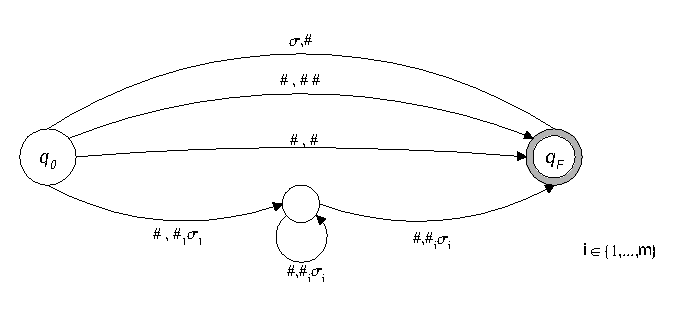
\includegraphics{img/pcgsgs/pcgsgs1}
    \caption{Časť 1-a-prekladača pre fázu inicializácie}\label{pcgsgs1}
  \end{figure}

    Najskôr $G$ uhádne počet komunikácií uskutočnených pri
    generovaní slova $w$ t.j. z koľkých podslov pozostáva $w$. Toto
    bude $G$ simulovať tak, že vygeneruje príslušný počet neterminálov $\#$.
    Potom $G$ uhádne príslušnosť jednotlivých podslov ku gramatikám
    t.j. ktoré podslovo bolo vyrobené ktorou gramatikou. Podľa toho
    bude $G$ prepisovať $\#$ na $\#_i\sigma_i$ (akési zárodky budúcich podslov),
    teda takto reprezentované podslovo bolo v $\Gamma$ generované gramatikou
    $G_i$. Zrejme prvý neterminál $\#$ bude prepísaný na $\#_1\sigma_1$, keďže
    prvé podslovo vygenerovala $G_1$

    \item[Prepisovací krok] (obr.\ref{pcgsgs2})
  \begin{figure}[ht]
    \centering
    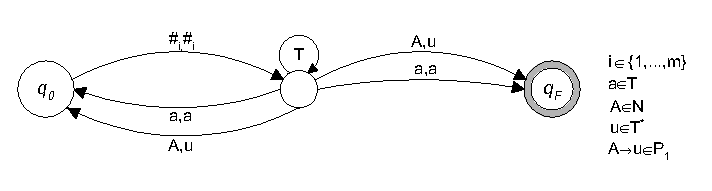
\includegraphics{img/pcgsgs/pcgsgs2}
    \caption{Časť 1-a-prekladača pre fázu prepisovania}\label{pcgsgs2}
  \end{figure}

    $g$-systémy vedia veľmi jednoducho simulovať regulárne
    gramatiky. V príslušnej vetnej forme skopírujú všetky
    neterminály a neterminál prepíšu podľa pravidiel regulárnej
    gramatiky. Náš $g$-systém $G$ bude vedieť simulovať všetky gramatiky
    $\Gamma$, pričom keď pri prechádzaní vetnej formy narazí na
    neterminál $\#_i$, bude simulovať gramatiku $G_i$ t.j. terminály
    sa skopírujú a neterminál sa prepíše podľa pravidiel v $G_i$.
    Môže sa stať, že vetná forma $G_i$ nebude obsahovať neterminál,
    preto musíme do $G$ pridať zopár šípok naviac, ktoré uhádnu, že
    nejaký terminál je vo vetnej forme danej gramatiky $G_i$
    posledný, aby sa nám nestalo, že v nejakom stave bude $G$
    na vstupe očakávať neterminál z $G_i$, ale dostane $\#_j$

    \item[Komunikačný krok] (obr.\ref{pcgsgs3})
  \begin{figure}[ht]
    \centering
    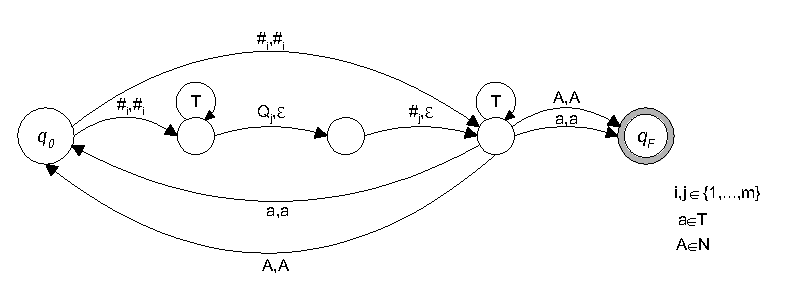
\includegraphics{img/pcgsgs/pcgsgs3}
    \caption{Časť 1-a-prekladača pre fázu komunikácie}\label{pcgsgs3}
  \end{figure}

    $G$ sa, predtým ako začne čítať vstup, niekedy rozhodne, že
    vo vetnej forme sa nachádzajú nejaké komunikačné symboly, teda
    má nastať komunikačný a nie prepisovací krok. $G$ uhádne podslovo,
    v ktorom sa nachádza komunikačný symbol $Q_j$ pre nejaké $j\in\{ 1\dots
    m\}$. Nech je toto podslovo generované gramatikou $G_k$. To znamená,
    že keď $G$ má na vstupe $\#_i$, môže sa
    rozhodnúť, či toto podslovo obsahuje alebo neobsahuje $Q_j$. Ak
    sa rozhodne, že nie, všetky terminály a prípadný neterminál
    skopíruje. Ak sa rozhodne, že áno, kopíruje terminály a očakáva
    $Q_j$. Ak sa objaví nejaký iný neterminál, znamená to, že $G$
    hádal nesprávne a zasekne sa. Ak na vstup príde $Q_j$, tak ho
    $G$ vymaže a očakáva symbol $\#_j$, ktorý tiež vymaže a zvyšok podslova
    skopíruje. Ak sa vo vetnej forme vyskytnú vedľa seba symboly
    $Q_j,\#_j$ znamená to, že v inicializácii $G$ správne uhádol
    následnosť týchto dvoch podslov t.j. uhádol, že gramatika $G_k$
    si vyžiada vetnú formu generovanú gramatikou $G_j$. Ak sa vo vetnej
    forme vyskytne dvojica $Q_j\#_i$ pre $j\neq i$, tak $G$ v inicializácii hádal
    zlú následnosť podslov a zasekne sa. Treba si uvedomiť, že toto
    naozaj simuluje komunikáciu, lebo v ďalšom prechode tým, že sme vymazali
    $Q_j\#_j$, bude podslovo pôvodne generované $G_j$ už súčasťou
    podslova generovaného $G_k$, a teda aj prepísanie prípadného
    neterminálu druhého podslova bude podliehať simulácii pravidiel
    $G_k$
    \item[Overovanie]
     V doterajšej simulácii sme ešte neuvažovali situáciu, že dve rôzne
    gramatiky $G_k,G_l$ $k\neq l$ naraz v tom istom kroku vygenerujú
    $Q_j$ pre nejaké $j\in \{ 1\dots m\}$. V $\Gamma$ to znamená, že
    vo vetnej forme oboch gramatík sa objaví ten istý obsah vetnej
    formy gramatiky $G_j$. V doteraz uvažovanej simulácii máme
    zabezpečené, že $G$ v inicializácii dobre uhádne dvojice
    $\#_k\sigma_k\#_j\sigma_j$ a $\#_l\sigma_l\#_j\sigma_j$, ale
    nemáme nijako zabezpečené, že simulácie odvodení gramatiky $G_j$
    budú na dvoch miestach rovnaké. Preto komunikačný krok upravíme
    nasledovne. $G$ si bude počas komunikačného kroku v stave pamätať
    $query$, ktoré už úspešne odstránil, a ak nájde vo vetnej forme
    ďalší taký symbol, zasekne sa. Tým sme zabezpečili,
    že komunikačný krok sa vykonaná len vtedy, keď vo vetnej forme
    nie sú viacnásobné $query$.
    \\ Keď sa $G$ rozhodne, že vo vetnej forme je viacnásobný
    $query$, tak uhádne a v stave si zapamätá $Q_j$, ktorý je
    viacnásobný a na začiatok vetnej formy dá špeciálny znak, upozorňujúci,
    že táto vetná forma je v stave overovania. Potom prehľadáva
    (kopíruje symboly) vetnú formu, a keď nájde prvý $Q_j$, tak ho
    vymaže, očakáva $\#_j$ ten tiež vymaže, v stave si zapamätá
    nasledujúci symbol podslova (pôvodne začínajúceho $\#_j$) a za
    tento symbol umiestni opäť špeciálny symbol $\pounds$ ukazujúci pokiaľ
    prečítal prvé overované podslovo. Zvyšok podslova skopíruje a v
    ďalších podslovách hľadá $Q_j$. Ak v podslove $Q_j$ nenájde, tak
    ho celé skopíruje, inak ho opäť vymaže spolu s očakávaným $\#_j$
    a porovnáva nasledujúci symbol podslova s tým, ktoré si
    zapamätal. Ak sa zhodujú, za tento symbol umiestni špeciálny
    znak $\$$ ukazujúci pokiaľ už podslovo overil a zvyšok podslova
    skopíruje, inak sa zasekne. Takto $G$ prejde celú vetnú formu.
    \\ Pri ďalšom prechode je na začiatku vstupu špeciálny symbol,
    ktorý hovorí, že máme pokračovať v overovaní. $G$ kopíruje
    symboly, až kým nenájde $\pounds$. Ten vymaže, zapamätá si ďalší
    symbol z overovaného podslova a zaň umiestni $\pounds$, zvyšok
    podslova skopíruje. V ďalších podslovách hľadá $\$$, a keď ho
    nájde, vymaže ho, skontroluje nasledujúci symbol so zapamätaným
    (ak sa nezhoduje, zasekne sa) a zapíše $\$$. Takýmto spôsobom
    dokáže $G$ overiť zhodnosť podslov, ktoré si dve gramatiky
    presunú do svojej vetnej formy, keď naraz vygenerujú rovnaké
    $query$.
    \\ $G$ sa niekedy na začiatku ďalšieho prechodu môže rozhodnúť,
    že už je overené celé podslovo t.j. za symbolmi $\pounds$, $\$$
    je nejaký $\#_i$. Vtedy $G$ vymaže špeciálny symbol na začiatku
    a symboly $\pounds$, $\$$ vo vetnej formy pričom overuje, či za
    týmito symbolmi sú naozaj nejaké $\#_i$, inak sa zasekne

    \item[Ukončenie] (obr.\ref{pcgsgs4})

  \begin{figure}[ht]
    \centering
    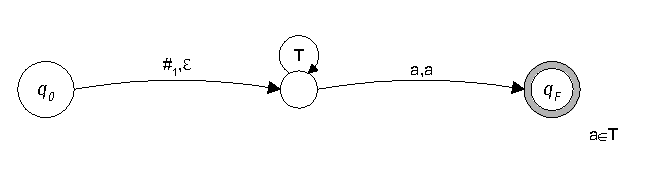
\includegraphics{img/pcgsgs/pcgsgs4}
    \caption{Časť 1-a-prekladača pre fázu ukončenia}\label{pcgsgs4}
  \end{figure}

    $G$ sa v počiatočnom stave niekedy rozhodne, že vetná forma
    obsahuje symbol $\#_1$ na začiatku a potom už len terminály. To znamená,
    že už nebudú nasledovať ani prepisovacie ani komunikačné kroky, teda simulácia
    $\Gamma$ už skončila. V tomto kroku stačí odstrániť symbol
    $\#_1$, čím dostaneme terminálne slovo
  \end{description}
  Čitateľ si určite všimol, že najzložitejšia z fáz bolo
  overovanie\footnote{preto sme ani neuviedli príslušný obrázok
  1-a-prekladača, ktorý by bol značne neprehľadný}. Skúsme sa preto
  zamyslieť, čo by sa stalo, keby sme overovanie zo simulácie
  vynechali. V takomto prípade sa však musíme obmedziť na
  simulovanie $PCGS$ s komunikačnou štruktúrou, ktorá nedovoľuje,
  aby v orientovanom grafe reprezentujúcom túto štruktúru existovali
  dve rôzne hrany vedúce do jedného vrchola. To napríklad spĺňajú
  štruktúry one-way array, one-way ring, tree, centr. Ak $\Gamma$ s
  takouto komunikačnou štruktúrou vygeneruje slovo v čase $T(n)$,
  tak $G$ vygeneruje toto slovo v rovnakom čase, teda $g$-systém
  zachováva časovú zložitosť $PCGS$.
  \\ Ak sa vrátime späť k všeobecnej komunikačnej štruktúre,
  overovanie zhorší časovú zložitosť polynomiálne
\end{dokaz}

\chapter{Alternujúce stroje}

V predchádzajúcich kapitolách sme si ukázali viaceré paralelné
modely. I keď šlo \mbox{o rôzne} pohľady na paralelizmus, všetky
mali jedno spoločné: pozerali sa na vec z ``gramatikového''
pohľadu, teda vo všetkých prípadoch sme mali jednu, prípadne
viacero gramatík, ktoré čosi generovali. Teraz si ukážeme jednu
automatovú charakterizáciu a porovnáme ju so sekvenčnými triedami.
Pre čitateľa, ktorý sa s pojmom alternovania ešte nestretol,
povedzme nasledovných pár viet. Modely alternujúcich strojov sa
uvažujú pre všetky známe zariadenia, my si ich popíšeme na
najvšeobecnejšom prípade, teda na Turingových strojoch, pre
čitateľa iste nebude problémom analogicky si zadefinovať
alternujúce konečné automaty, alternujúce zásobníkové automaty,
prípadne alternujúce lineárne ohraničené automaty. O niektorých
týchto zariadeniach si v závere kapitoly ukážeme pár zaujímavých
vecí, napr. ako alternovanie ovplyvní, resp. neovplyvní ich
generatívnu silu a podobne. Zariadenie (alternujúci stroj) má tzv.
existenčné a tzv. univerzálne stavy, ktoré môže ľubovoľne
kombinovať, a ktoré si ďalej bližšie popíšeme. Alternujúci
Turingov stroj sa v existenčných stavoch správa rovnako, ako už
známy nedeterministický model Turingovho stroja. Odlišné je
správanie sa v univerzálnych stavoch. Zariadenie sa akoby rozdelí
na $n$ nových strojov (kde $n$ je počet konfigurácií
dosiahnuteľných na 1 krok z jeho momentálnej konfigurácie), ktoré
dostanú novú pamäť (rovnakú ako pôvodný stroj) a ďalej nezávisle
od seba pracujú, táto operácia sa nazýva FORK a čitateľovi môže
byť trošku v reálnejšej podobe známa z niektorých operačných
systémov (UNIX), kde jeden proces vytvára nové a prideľuje im
pamäť.

\section{Definície a označenia}

\begin{definicia}
  Alternujúci Turingov stroj (ATS) je 6-tica
  $A=(K,\Sigma,\Gamma,\delta,q_0,F)$, kde $K$ je konečná množina
  stavov rozdelená na dve disjunktné časti $K=K_1\cup K_2$, $K_1$ je
  množina exis\-tenčných stavov, $K_2$ je množina univerzálnych
  stavov, $\Sigma$ je abeceda vstupných symbolov, $\Gamma$ je
  pracovná (pásková) abeceda, $q_0$ je počiatočný stav a $F$ je
  množina akceptačných stavov, $\delta$ je prechodová funkcia
  \[
  \delta:K\times\Gamma\ra 2^{K\times\Gamma\times\{-1,0,1\}}
  \]
\end{definicia}

\begin{definicia}
  Konfiguráciu ATS $A$ definujeme rovnako ako pre nedeterministické
  Turingove stroje (NTS), bližšie napr. \cite{Hopc}
\end{definicia}

\begin{definicia}
  Krok výpočtu ATS $A$ je relácia $\vdash$ na konfiguráciách
  definovaná rovnako ako pre NTS
\end{definicia}

Čitateľ si možno spomenie na pojem stromu konfigurácií, definovaný
pre nedeterministický Turingov stroj, ktorý prehľadne
reprezentoval jeho výpočet na konkrétnom slove\footnote{bol napr.
dobrou pomôckou pri dôkaze ekvivalencie deteministických a
nedeterministických Turingových strojov}. Podobný strom definujeme
aj pre alternujúce stroje. Okrem toho, že nám tento pojem pomôže
pri definovaní výpočtu ATS, mal mi výraznou mierou prispieť k
pochopeniu alternovania samotného.

\begin{definicia}
  Úplný strom konfigurácií pre ATS $A$ a vstupné slovo $w$ je strom,
  ktorého vrcholy sú označené konfiguráciami taký, že:
  \begin{enumerate}
    \item koreň je počiatočná konfigurácia na slove $w$
    \item každý vrchol má za priamych nasledovníkov práve toľko
      vrcholov, koľko konfigurácii je v relácii $\vdash$ s konfiguráciou
      označujúcou daný vrchol
    \item tieto vrcholy sú označené týmito konfiguráciami
  \end{enumerate}
\end{definicia}

\begin{poznamka}
  Úplný strom konfigurácií nemusí byť konečný
\end{poznamka}

\begin{definicia}
  Výpočet ATS $A$ (na slove $w$) je podstrom úplného stromu
  konfigurácií na slove $w$ taký, že:
  \begin{enumerate}
    \item obsahuje koreň
    \item s každým univerzálnym vrcholom $(q\in K_2)$ obsahuje
      všetkých jeho priamych nasledovníkov
    \item s každým existenčným vrcholom obsahuje práve jedného jeho
      priameho nasledovníka, ak existuje
  \end{enumerate}
\end{definicia}

\begin{definicia}
  Akceptujúci výpočet ATS $A$ na slove $w$ je taký výpočet na $w$,
  ktorý je konečný a každá listová konfigurácia je akceptačná
\end{definicia}

\begin{definicia}
  Jazyk akceptovaný ATS $A$ je
  \[
  L(A)=\{w\in\Sigma^*\mm \mbox{existuje akceptačný výpočet}\ A\
  \mbox{na}\ w\}
  \]
\end{definicia}

\begin{priklad}\label{dvojhlavy}
  Ukážeme si, ako alternovanie pomôže dvojhlavým konečným
  automatom\footnote{budeme uvažovať zariadenie s možnosťou pohybu
  hlavy iba jedným smerom} v ge\-ne\-ra\-tív\-nej sile. Zoberme si
  jazyk $L=\{ww\mm w\in\{a,b\}^*\}$. Dalo by sa ukázať, že ho nie je
  možné akceptovať dvojhlavým konečným automatom, no zostrojíme preň
  alternujúci dvojhlavý konečný automat, ktorý bude pracovať
  nasledovne:
  \begin{enumerate}
    \item dostane na vstup slovo, nedeterministicky uhádne jeho
    polovicu
    \item nastane FORK, automat alternuje v univerzálnom stave
    \begin{itemize}
      \item 1. proces overuje, či vstup je tvaru $ww$ tak, že hlavy sa
        synchrónne pohybujú po vstupe, v jednom kroku každá číta symbol,
        ak obe prečítajú to isté a keď sa jedna z nich dostane na koniec
        vstupu, dôjde k akceptovaniu
      \item 2. proces overuje, či automat uhádol polovicu správne tak,
        že prvá hlava sa hýbe o jedno políčko vpravo, zatiaľ čo za ten
        istý čas sa druhá hlava hýbe o dve políčka vpravo, k akceptovaniu
        dôjde, ak obe hlavy dočítajú naraz vstupné slovo
    \end{itemize}
  \end{enumerate}
  Výpočet automatu možno vidieť na (obr.\ref{apreww})
\end{priklad}

\begin{figure}[!ht]
  \centering
  \includegraphics{img/apreww}
  \caption{Úplný strom konfigurácií automatu pre jazyk $L=\{ww\mm
  w\in\{a,b\}^*\}$} z príkladu \ref{dvojhlavy} \label{apreww}
\end{figure}

\begin{veta}
  $\Langclass{ATS} = \Langclass{RE}$
\end{veta}

\begin{dokaz}
  Povieme si pár slov o oboch inklúziách:
  \begin{description}
    \item{$\subseteq$:} vyplýva z Turingovej tézy, keby sme mali
      zkonštruovať TS, ktorý by simuloval ATS, tak by sme zrejme
      prechádzali strom konfigurácii ATS do šírky, pamätali si niečo o
      výpočte a charaktere stavov a podobne
    \item{$\supseteq$:} na NTS sa možno pozerať aj ako na špeciálny
      prípad ATS, keď akoby všetky stavy NTS boli existenčné
  \end{description}
\end{dokaz}

\section{Miery zložitosti}

Pre ATS si zadefinujeme dve miery, ktoré sú analógiou mier
$NSPACE,NTIME$ definovaných pre NTS:

\begin{itemize}
  \item $ASPACE=$ najväčší počet použitých políčok na páske v
    niektorej konfigurácii akceptačného výpočtu
  \item $ATIME=$ hĺbka akceptačného výpočtu v strome
    konfigurácií
\end{itemize}

V niektorých simuláciách budeme pracovať s triedou jazykov
$ATIME(f(n))$, $\log n<f(n)<n$. Klasický model ATS by sme tu
nemohli použiť, lebo na prečítanie vstupu dĺžky $n$ potrebujeme
aspoň $n$ krokov. V takýchto prípadoch sa používa model ATS s
rýchlym prístupom na vstup. Môžeme si ho reprezentovať nasledovne:
nad páskou má binárny vyhľadávací strom, každý list je práve jedno
políčko, strom má výšku $\log n$, máme register dĺžky $\log n$,
keď do neho binárne zapíšeme číslo $k$, tak za čas $\log n$ sa
dostaneme ku $k$-temu vstupnému políčku (obr.\ref{rychly}).

\begin{figure}[!ht]
  \centering
  \includegraphics{img/rychly}
  \caption{Model ATS s rýchlym prístupom na vstup} \label{rychly}
\end{figure}

\section{Alternujúce vs. sekvenčné triedy zložitosti}

Keďže vo väčšine simulácií budeme požadovať predpoklad páskovej
konštruovateľnosti nejakej funkcie, bude dobré, keď si tento pojem
zadefinujeme.

\begin{definicia}
  Funkcia $f(n)$ sa nazýva páskovo konštruovateľná, ak existuje
  deterministický Turingov stroj (DTS) $T$, ktorý je $f(n)$ páskovo
  ohraničený a vyznačí na páske $f(n)$ políčok
\end{definicia}

Ukazuje sa, že takmer všetky funkcie, ktoré si možno reálne
predstaviť, sú páskovo konštruovateľné, problémy pri
konštruovateľnosti však nastávajú, keď sa pozrieme na triedu
funkcií menších ako $\log n$, teda $O(\log n)$. Keby sme chceli
nahliadnuť medzi nekonštruovateľné funkcie, dobrým prostriedkom na
ich zostrojovanie by bola metóda diagonalizácie.

\smallskip
V tejto chvíli sme už pripravení na ukázanie základného výsledku o
alternujúcich Turingových strojoch.

\begin{veta}
  \label{alter_veta_nspaceatime}
  $NSPACE(S(n))\subseteq ATIME(S^2(n))$ pre
  $S(n)\geq\log n$
\end{veta}

\begin{dokaz}
  Ak $S(n)\geq n$, nie je problém v lineárnom čase prečítať vstup,
  ak by však bolo $S(n)<n$, na prečítanie vstupu našim ATS $A'$ by
  sme potrebovali aspoň lineárny čas a celá simulácia by ztroskotala
  už na začiatku. Preto použijeme model ATS s rýchlym prístupom na
  vstup, v logaritmickom čase $O(\log n)$ sa vieme dostať na
  ľubovoľné políčko vstupnej pásky, využívame tu ideu paralelnej
  práce procesov, nie každý proces musí vidieť celý vstup, aby
  akceptoval, resp. každému procesu bude k práci stačiť malý úsek
  vstupu. K danému NTS $A$ pracujúcemu v priestore $S(n)$ zostrojíme
  ATS $A'$ pracujúci v čase $S^2(n)$ taký, že $L(A)=L(A')$.

  \smallskip
  Akceptujúci výpočet $A$ na slove $w$ dĺžky $n$ má (zmysluplne)
  dĺžku najviac $c^{S(n)}$ pre vhodné\footnote{ako už neraz,
  $c^{S(n)}$ je počet rôznych konfigurácií $A$ na slove dĺžky $n$,
  keď máme k dispozícii priestor $S(n)$} $c$. Položme $m=c^{S(n)}$,
  $\forall i\med k_i$ je konfigurácia $A$, akceptujúci výpočet má
  tvar:
  \[
  k_1\vdash k_2\vdash\dots\vdash k_m
  \]
  pričom $k_1$ je počiatočná konfigurácia, $k_m$ je akceptačná
  konfigurácia (ak je náhodou akceptujúci výpočet kratší,
  dodefinujeme $\delta$-funkciu v akceptačnom stave tak, aby sa nič
  nedialo, ale aby sme mohli ``naťahovať'' výpočet).

  \smallskip
  ATS $A'$ bude pracovať nasledovne:
  \begin{enumerate}
    \item výpočet začne v $k_1$
    \item uhádne akceptačnú konfiguráciu $k_m$
    \item overí, či sa z $k_1$ do $k_m$ dá dostať na $m$ krokov
      nasledovne:
      \begin{enumerate}
        \item uhádne $k_{\frac{m}{2}}$
        \item overí, či sa z $k_1$ dá dostať do $k_{\frac{m}{2}}$ na $\frac{m}{2}$
        krokov
        \item overí, či sa z $k_{\frac{m}{2}}$ dá dostať do $k_m$ na $\frac{m}{2}$
        krokov
      \end{enumerate}
  \end{enumerate}
  Body b) a c) tretieho kroku sú vlastne rekurzívne volania kroku 3
  s parametrami $k_1,k_{\frac{m}{2}},\frac{m}{2}$, resp.
  $k_{\frac{m}{2}},k_m,\frac{m}{2}$. ATS $A'$ sa do rekurzie bude
  vnárať\footnote{každé rekurzívne volanie si môžme reprezentovať z
  hľadiska alternovania tak, že $A'$ vytvorí nový proces, ktorý ako
  parametre dostane $k_i,k_j,r$ a za úlohu má overiť, či sa z $k_i$
  dá dostať do $k_j$ na $r$ krokov (obr.\ref{ats_time})} dovtedy,
  kým sa nedostane na úroveň, kedy bude overovať, či sa dá z $k_i$
  dostať do $k_{i+1}$ na jeden krok $\forall i=1,\dots,m-1$
  (obr.\ref{aspace1}). Táto úroveň je z hľadiska rekurzie
  elementárna, na nej stačí overiť, či v $\delta$-funkcii NTS $A$
  existoval taký prechod, ktorý umožnil prepísanie konfigurácie
  $k_i$ na $k_{i+1}$ (teda simulujeme jeden krok pôvodného NTS $A$).
  Je nutné si uvedomiť, že rekurzia sa vykonáva paralelne.

  \begin{figure}[!ht]
    \centering
    \includegraphics{img/aspace1}
    \caption{Overovanie náveznosti konfigurácií v ATS $A'$}
    \label{aspace1}
  \end{figure}

  Pozrime sa na proces hádania konfigurácií a overovania
  dosiahnuteľnosti konfigurácie $k_j$ z konfigurácie $k_i$ na $m$
  krokov podrobnejšie, z hľadiska alternovania a rozdelenia množiny
  stavov ATS $A'$ na existenčné a univerzálne. Na začiatku výpočtu
  je $A'$ v stave $q_0$ a na vstupe má slovo $w$, teda $k_1=q_0 w$,
  tento stav je existenčný. Teraz $A'$ prejde do stavu $q_H$ a háda
  $k_m$, pod $q_0 w$ v strome konfigurácií visí ``veľmi košatý''
  strom (označme ho $N$), je na (obr.\ref{strom_n}), výšky $S(n)$,
  ktorý ako všetky svoje vrcholy, vrátane listov, obsahuje všetky
  možné konfigurácie NTS $A$ v priestore $S(n)$. Kvôli jednoduchosti
  si ho môžeme popísať nasledovne\footnote{konfigurácia ako ju
  popisujeme, neobsahuje stav, ani pozíciu hlavy, čitateľ si tieto
  veci iste rád domyslí sám} (na čitateľa nechávame domyslenie
  ukončenia generovania):
  \[
  \delta(q_H,1)=\{(q_H,a,1),(q_H,b,1)\}
  \]

  \begin{figure}[!ht]
    \centering
    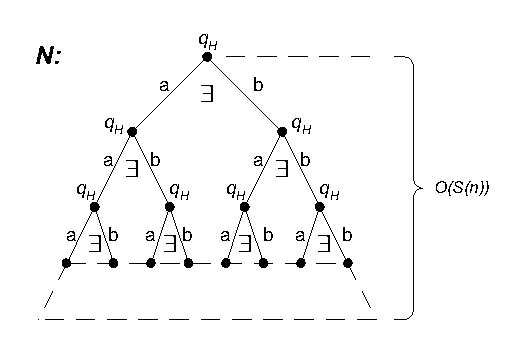
\includegraphics{img/strom_n}
    \caption{Hádanie konfigurácie dĺžky $S(n)$ ATS $A'$}
    \label{strom_n}
  \end{figure}

  Keď má $A'$ uhádnutú akceptačnú konfiguráciu $k_m$, overí, či sa z
  $k_1$ do $k_m$ dá dostať na $m$ krokov. To spraví tak, že uhádne
  $k_{\frac{m}{2}}$ rovnako, ako hádal $k_m$ (teda pod každým
  vrcholom stromu $N$ visí nový strom (opäť rovnaký ako $N$, má
  odlišné stavy, všetky sú existenčné), v ktorom $A'$ háda
  $k_\frac{m}{2}$). Keď ju uhádne, overuje, či sa z $k_1$ dá dostať
  do $k_{\frac{m}{2}}$ na $\frac{m}{2}$ krokov a či sa z
  $k_{\frac{m}{2}}$ dá dostať do $k_m$ na $\frac{m}{2}$ krokov tak,
  že v univerzálnom stave spraví FORK dvoch nových
  procesov\footnote{to je práve jedno rekurzívne volanie}, ktoré
  pracujú paralelne a každý overuje polovicu toho, čo mal overiť
  materský proces, atď.

  \begin{figure}[!ht]
    \centering
    \includegraphics{img/ats_time}
    \caption{Schématické vytváranie nových procesov ATS $A'$}
    \label{ats_time}
  \end{figure}

  Z konštrukcie by malo byť zrejmé (nebudeme to dokazovať), že
  $L(A)=L(A')$. Poďme sa teraz pozrieť na časovú zložitosť ATS $A'$,
  ktorý sme práve zkonštruovali: máme $O(S(n))$ rekurzívnych volaní
  a v každom hádame strednú konfiguráciu, resp. na začiatku musíme
  uhádnuť akceptačnú konfiguráciu $k_m$. Hádanie ľubovoľnej
  konfigurácie $k_i$ trvá čas $O(S(n))$, čo je presne výška stromu
  $N$, lebo ju treba zapamätať na páske. Celkový počet krokov (alebo
  inak výška akceptačných vetiev úplného stromu konfigurácií) $A'$
  je $O(S^2(n))$ a teda $L(A')\in ATIME(S^2(n))$
\end{dokaz}

\begin{poznamka}
  V predchádzajúcej vete sme použili ``paralelnú verziu''
  konštrukcie, ktorá bola (v sevkvenčnej podobe) použitá pri dôkaze
  vety $NSPACE(S(n))\subseteq DSPACE(S^2(n))$ (Savitch)
\end{poznamka}

Pri väčšine známych konštrukcií, keď máme dané zariadenie
(Turingov stroj) a požadujeme k nemu zostrojiť zariadenie
ekvivalentné, ale rýchlejšie, urýchlenie ide na úkor použitého
priestoru, resp. analogicky keď požadujeme zmenšenie použitého
priestoru, ide to na úkor času. Ako naznačila konštrukcia z vety
\ref{alter_veta_nspaceatime}, pri alternujúcich strojoch je situácia trochu
iná. Pozornému čitateľovi iste neunikol fakt, že priestorové
ohraničenie zostrojeného ATS zostalo nezmenené.

\smallskip
V niektorých konštrukciách bude kôli jednoduchosti vhodné uvažovať
binárne vetvenie úplného stromu konfigurácií ATS, teda fakt, že
ľubovoľný prechod $\delta$-funkcie má najviac dva prvky. Ukážeme
si preto nasledovné dve tvrdenia o normálnych tvaroch pre ATS.

\begin{lema}\label{binarny_nt}
  K ľubovoľnému ATS $A$ pracujúcemu v čase $T(n)$ s ľubovoľnou
  veľkosťou vetvenia\footnote{veľkosťou vetvenia rozumieme maximálny
  počet konfigurácii dosiahnuteľný z ľubovoľnej konfigurácie na
  jeden krok} v úplnom strome konfigurácii existuje ATS $A'$
  pracujúci v čase $T(n)$, ktorého úplný strom konfigurácii je
  binárny a $L(A)=L(A')$
\end{lema}

\begin{dokaz}
  Iba neformálne naznačíme spôsob konštrukcie $A'$: nech je vetvenie
  vo vrchole $v$ úplného stromu konfigurácií $A$ stupňa $n$. Binárne
  vetvenie vytvoríme tak, že v ľavej vetve vychádzajúcej z vrchola
  $v$ bude jeho najľavejší nasledovník a v pravej všetci ostatní
  nasledovníci tak, že priamy nasledovník $v$ bude $v'$ a jeho
  nasledovníci budú zvyšnými nasledovníkmi $v$. Konfiguráciu v tomto
  vrchole dostaneme tak, že v konfigurácii vo $v$ zmeníme stav na
  nový, ktorý ešte nepatrí do množiny stavov $A$, vetvenie vrchola
  $v'$ bude stupňa $n-1$, teda o 1 menšieho ako vetvenie $v$. Na
  vrchol $v'$ aplikujeme algoritmus rekurzívne a v rekurzii skončíme
  až vtedy, keď bude vrchol stupňa $\leq2$. Na čitateľa nechávame
  premysieť, ako algoritmus aplikovať na celý strom
  konfigurácií\footnote{pomôcka: $\delta$-funkcia $A$ má iba konečne
  veľa prvkov a vetvenie v úplnom strome konfigurácií je iba
  grafické znázornenie $\delta$-funkcie, resp. výpočtu}. Dodajme
  ešte, že ak vrchol $v$ bol existenčný, tak aj všetky vrcholy,
  ktoré pri vytváraní binárneho vetvenia vzniknú, budú existenčné,
  podobne ak $v$ bol univerzálny, tak všetky vzniknuté vrcholy budú
  univerzálne. Uvedomme si, že hĺbka akceptačného výpočtu v úplnom
  strome konfigurácií $A'$ bude iba konštantným násobkom hĺbky
  úplného stromu konfigurácií $A$, teda $A'$ pracuje v čase $T(n)$ a
  akceptuje rovnaký jazyk ako $A$
\end{dokaz}

\begin{lema}\label{binarny_nt2}
  K ľubovoľnému ATS $A$ pracujúcemu v priestore $S(n)$ s ľubovoľnou
  veľkosťou vetvenia v úplnom strome konfigurácii existuje ATS $A'$
  pracujúci v priestore $S(n)$, ktorého úplný strom konfigurácii je
  binárny a $L(A)=L(A')$
\end{lema}

\begin{dokaz}
  V konštrukcii z lemy \ref{binarny_nt} sme nikde nemenili priestor,
  ktorý využíval $A$ pri práci, a teda tvrdenie je jej priamym
  dôsledkom
\end{dokaz}

Nasledujúce tvrdenie hovorí, ako efektívne z hľadiska
priestorového ohraničenia vieme simulovať alternujúce Turingove
stroje pracujúce v čase $T(n)$ na deterministických Turingových
strojoch.

\begin{veta}
  \label{atimedspace} $ATIME(T(n))\subseteq DSPACE(T(n))$ pre
  $T(n)\geq\log n, T(n)$ je páskovo konštruovateľná
\end{veta}

\begin{dokaz}
  V celom dôkaze budeme pod pojmom strom konfigurácii rozumieť
  podstrom úplného stromu konfigurácii, ktorý dostaneme tak, že v
  úplnom strome konfigurácii ``odrežeme'' všetky vetvy v hĺbke
  $T(n)$.

  \smallskip
  K danému ATS $A$ pracujúcemu v čase $T(n)$ zostrojíme DTS $A'$
  pracujúci v priestore $T(n)$. Podľa lemy \ref{binarny_nt} môžeme
  kvôli jednoduchosti predpokladať, že úplný strom konfigurácii $A$
  je binárny. $A'$ musí overiť, či sa v strome konfigurácií $A$
  nachádza podstrom akceptujúceho výpočtu.

  \smallskip
  $A'$ bude prehľadávať strom konfigurácií $A$ algoritmom PREORDER
  do hĺbky a priradzovať vrcholom hodnoty $0,1$ nasledovne:
  \begin{itemize}
    \item vrcholu sa môže priradiť hodnota iba vtedy, ak sú už
      priradené hodnoty všetkým jeho nasledovníkom v strome konfigurácii
      alebo ak je to list\footnote{listom sa v tomto prípade myslí aj
      taký vrchol, ktorý síce nie je listovým v úplnom strome
      konfigurácii $A$, ale stáva sa listovým vrcholom v strome
      konfigurácii $A$}
    \item listom priradzujeme hodnoty podľa toho, či sú akceptujúcimi,
      alebo neakceptujúcimi konfiguráciami, akceptujúcim priradíme
      hodnotu 1, neakceptujúcim hodnotu 0
    \item ak je vrchol existenčný (a nie je to list)
      a aspoň jeden z jeho nasledovníkov v strome konfigurácii má
      hodnotu $1$, tak sa mu priradí hodnota $1$, inak sa mu priradí $0$
    \item ak je vrchol univerzálny (a nie je to list), tak sa mu priradí
      hodnota 1 práve vtedy, keď obaja jeho nasledovníci v strome
      konfigurácií majú hodnotu 1, inak sa mu priradí 0
  \end{itemize}
  $A'$ akceptuje svoj vstup práve vtedy, keď bude koreňu priradená
  hodnota 1. Keby sme chceli dosiahnuť dobrý pomer čas/priestor, asi
  by sme postupovali tak, že by sme si pamätali informáciu o celom
  ``lúči'' konfigurácii, teda všetky konfigurácie, ktorými sme od
  koreňa prechádzali až k listom, resp. ku vrcholom v hĺbke $T(n)$,
  aby sme nestrácali čas pri vracaní sa v strome smerom nahor.
  Dosiahli by sme však priestorové ohraničenie $T^2(n)$ (pretože by
  sme si museli pamätať až $T(n)$ konfigurácií, každú dĺžky $T(n)$),
  čo v našom prípade nie je žiadúce, preto budeme musieť použiť
  trochu rafinovanejšiu konštrukciu, vzhľadom na to, že nám nezáleží
  na čase. Nebudeme si pamätať celý ``lúč'' konfigurácii, ale iba
  momentálnu konfiguráciu a navigáciu k nej v strome konfigurácii.
  Navigácia bude dĺžky najviac $T(n)$ a bude to postupnosť z
  $\{0,1\}^*$, kde 0 znamená pohyb v strome vľavo smerom dole a 1
  znamená pohyb vpravo smerom dole. Keď sa budeme v strome musieť
  vracať smerom hore, tak si predchodcu konfigurácie, v ktorej práve
  sme, podľa tejto navigácie vypočítame, na páske $A'$
  (obr.\ref{paska}) si budeme potrebovať pamätať navigáciu,
  momentálnu konfiguráciu a pár pomocných konfigurácii, teda máme
  priestorové ohraničenie $T(n)$ pre $A'$
\end{dokaz}

\begin{figure}[!ht]
  \centering
  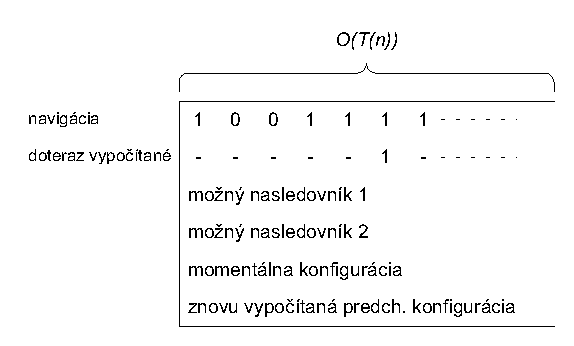
\includegraphics{img/paska}
  \caption{Páska DTS $A'$ (druhá stopa by sa dala pamätať aj v
  stave)} \label{paska}
\end{figure}

\begin{definicia}
  Polynomiálne triedy zložitosti definujeme nasledovne:
  \begin{itemize}
    \item $NSPACE(Poly)\overset{def}=\underset{{k\geq1}}{\bigcup}NSPACE(n^k)$
    \item $DSPACE(Poly)\overset{def}=\underset{{k\geq1}}{\bigcup}DSPACE(n^k)$
    \item $ATIME(Poly)\overset{def}=\underset{{k\geq1}}{\bigcup}ATIME(n^k)$
  \end{itemize}
\end{definicia}

\begin{dosledok} \label{alter_dosl_nspacepolyatimepoly}
  $NSPACE(Poly)=DSPACE(Poly)=ATIME(Poly)$
\end{dosledok}

\begin{dokaz}
  Tvrdenie vyplíva zo Savitchovej vety, vety \ref{alter_veta_nspaceatime} a
  vety \ref{atimedspace}
\end{dokaz}

\begin{veta}
  $ASPACE(S(n))\subseteq\underset{{c>0}}{\bigcup}DTIME(c^{S(n)})$
  pre $S(n)\geq\log n$
\end{veta}

\begin{dokaz}
  Ukážeme si, že keď máme k ATS $A$ pracujúcemu v priestore $S(n)$
  zostrojiť DTS $A'$ pracujúci v exponenciálnom čase $c^{S(n)}$ pre
  nejaké nezáporné $c$, tak nám na simuláciu postačí aj veľmi hrubá
  sila, akou je bezosporu vygenerovanie všetkých možných
  konfigurácii $A$ na páske a práca na týchto konfiguráciách. Opäť
  budeme bez újmy na všeobecnosti predpokladať, že úplný strom
  konfigurácií $A$ je binárny.

  \smallskip
  $A'$ bude pracovať nasledovne:
  \begin{itemize}
    \item na pásku zapíše všetkých $|\Gamma_A|^{S(n)}.S(n).|K_A|<r^{S(n)}$
      konfigurácii $A$ v lexikografickom usporiadaní, za každou
      konfiguráciou si nechá priestor (jedno políčko), ktorý ďalej
      využije\footnote{priestor si na páske vyznačíme napr. $\#?\#$,
      pričom $\#$ slúži ako oddeľovač konfigurácii, nie je prvkom
      páskovej abecedy $\Gamma$, rovnako ani $?$, ktorý hovorí, že o
      tomto políčku zatiaľ nič nevieme}, na to potrebuje čas
      $S(n).r^{S(n)}$
    \item do vyznačeného priestoru bude každej konfigurácii
      priraďovať hodnoty $0,1,?$ prechodom stromu konfigurácii $A$ tak,
      že v každom prechode priradí hodnoty $0,1$ rodičom tých detí,
      ktoré už sú vyhodnotené a hodnotu $?$ rodičom nevyhodnotených detí
      (podľa (obr.\ref{exponent})), akceptuje, ak bude počiatočnej
      konfigurácii priradená hodnota $1$, časová zložitosť bude
      nasledovná:
      \begin{enumerate}
        \item $r^{S(n)}$-krát prejde pásku a ``spracuje'' každú konfiguráciu
        \item ``spracovať'' konfiguráciu znamená zistiť hodnoty jej
          nasledovníkov a ak sa dá, tak jej priradiť hodnotu 0,1, toto je
          časovo ohraničené $\approx r^{S(n)}.S(n)$
      \end{enumerate}
  \end{itemize}
  Keď si celú prácu $A'$ zosumarizujeme, dostávame časovú zložitosť
  približne $c^{S(n)}$ pre nejaké $c$ (stačí zvoliť napr.
  $c=r^{10}$) a sme hotoví
\end{dokaz}

\begin{figure}[!ht]
  \centering
  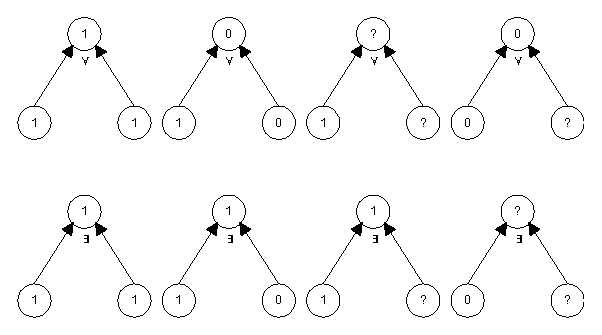
\includegraphics{img/exponent}
  \caption{Priraďovanie hodnôt rodičom v strome konfigurácii ATS
  $A$} \label{exponent}
\end{figure}

\begin{veta}
  \label{dtime_aspace}
  $DTIME(T(n))\subseteq ASPACE(\log T(n))$ pre $T(n)\geq n$
\end{veta}

\begin{dokaz}
  Nech $A_1$ je $k$-páskový DTS pracujúci v čase $T(n)$. K nemu
  existuje jednopáskový DTS $A=(K_A,\Sigma,\Gamma,\delta,q_0,F_A)$
  pracujúci v čase $T^2(n)$ taký, že $L(A_1)=L(A)$. K nemu
  zkonštruujeme ATS $A'$ pracujúci v priestore $\log T(n)$ taký, že
  $L(A)=L(A')$. Najskôr si zapíšme konfigurácie $A$ pod seba podľa
  (obr.\ref{dts_ats}) tak, že v prvom riadku bude počiatočná
  konfigurácia $q_0w$ a keď označíme $<qw_k>_{l}$ konfiguráciu v
  $k$-tom riadku pre nejaký stav $q\in K_A$ a pozíciu stavu (hlavy)
  v tejto konfigurácii $l$, tak platí
  $<qw_k>_{l}\vdash<pw_{k+1}>_{m}$, pričom $m\in\{l-1,l,l+1\}$. Ak
  $w\in L(A)$, tak máme v tabuľke zapísanú postupnosť konfigurácií
  akceptujúceho výpočtu (vzhľadom na to, že $A$ je deterministický),
  teda existuje $i$ také, že pre $<q_Fw_i>_j$ je $q_F\in F_A$.

  \begin{figure}[!ht]
    \centering
    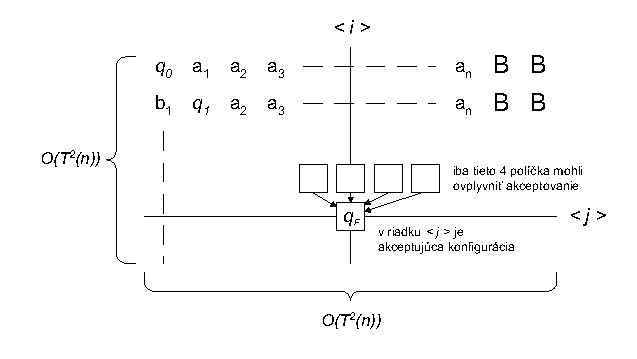
\includegraphics{img/dts_ats}
    \caption{Tabuľka konfigurácií jednopáskového DTS $A$}
    \label{dts_ats}
  \end{figure}

  $A'$ bude pracovať nasledovne:
  \begin{itemize}
    \item uhádne pozíciu $<$riadok, stĺpec$>$ akceptačného stavu $q_F$
      v akceptujúcej kon\-fi\-gu\-rá\-cii tvaru \mbox{$<q_Fw_i>_j$},
      teda háda $<i,j>$, toto zaberie $\log T^2(n)$ políčok (môžeme
      zvoliť napr. binárnu reprezentáciu čísel $i,j$), to je $2.\log
      T(n)\approx\log T(n)$ políčok
    \item uhádne, ktorý akceptujúci stav sa na pozícii $<i,j>$
      nachádza
    \item overí, či dobre hádal pozíciu $<i,j>$ a akceptačný stav
      nasledovne:
      \begin{enumerate}
        \item uhádne (zmysluplne\footnote{podľa $\delta$-funkcie $A$})
          obsahy políčok
          \mbox{$<i-1,j-1>,<i-1,j>,<i-1,j+1>$},\\\mbox{$<i-1,j+2>$}, pretože
          týmito obsahmi je obsah $<i,j>$ jednoznačne určený
        \item v univerzálnom vetvení overí, či hádal správne (každá
          vetva overí jedno políčko)
      \end{enumerate}
      Takto sa bude $A'$ vracať v tabuľke až do prvého riadku (zrejme si
      bude dekrementovať $i$ a pracovať s $j$ podľa pohybu hlavy $A$),
      keď bude na pozícii $<1,1>$ a bude v počiatočnom stave, tak
      akceptuje
  \end{itemize}
  Pri prechode tabuľkou konfigurácií smerom zdola nahor sa nám
  nemôže stať, že by sme našli viac ako jednu cestu vedúcu k
  akceptovaniu, pretože $A$ je deterministický a teda akceptačný
  výpočet pre dané slovo je vždy jednoznačný, ak sme v niektorej
  vetve niečo zle uhádli, výpočet sa určite zablokuje.

  \smallskip
  Keď sa máme baviť o priestorovej zložitosti $A'$, jediná vec,
  ktorá ju ovplyvňuje, je dĺžka $i$, resp. $j$, pretože okrem týchto
  dvoch čísel si pamätáme iba konštantne veľa informácii (dokonca
  veľmi málo). Ale o dĺžke sme si už povedali, že je $\log T(n)$,
  takže sme hotoví
\end{dokaz}

\begin{dosledok}
  $ASPACE(S(n))=\underset{{c>0}}{\bigcup}DTIME(c^{S(n)})$ pre
  $S(n)\geq n$
\end{dosledok}

\section{Alternujúce konečné automaty ($AFSA$)}

Čitateľ sa iste stretol s viacerými modifikáciami pôvodného modelu
deterministických konečných automatov. Nedeterminizmus im
nepomohol, rovnako ako nepomohlo napr. pridanie možnosti
obojsmerného pohybu po vstupnej páske. Mohlo by sa zdať, že taká
sila, akou je alternovanie, by mohlo pomôcť týmto zariadeniam
vyjsť z triedy $\Regclass$ a akceptovať aj nejaké nie regulárne
jazyky. Ako však hovorí nasledujúca veta, opak je pravdou. Faktom
totiž zostáva, že keď procesom v jednotlivých vetvách neumožníme
komunikáciu, resp. synchronizáciu, tak sa sila zariadenia
nezväčší.

\begin{veta}
  $\Langclass{AFSA} = \Regclass$
\end{veta}

\begin{dokaz}
  \label{afsa_r} Inklúzia zprava doľava je triviálna a preto ju
  nebudeme ukazovať. Na dôkaz opačnej inklúzie zostrojíme k AFSA $A$
  ekvivalentný nedeterministický konečný automat (NKA) $A'$ taký, že
  \mbox{$L(A)=L(A')$}. Najskôr podobnou konštrukciou ako pre NKA
  zostrojíme k $A$ ekvivalentný ATS $A_1$ (teda platí $L(A)=L(A_1)$)
  taký, že v $A_1$ neexistujú $\varepsilon$-prechody (konštrukcii sa
  nebudeme bližšie venovať, čitateľ ju nájde napr. v \cite{Hopc}).
  Zavedieme pár označení, ktoré sa nám neskôr budú hodiť:
  \begin{itemize}
    \item $all(q,a)=\{$množina všetkých stavov dosiahnuteľných v $A_1$ na
      jeden krok zo stavu $q$ pri čítaní vstupného symbolu $a\}$
    \item $ex_i(q,a)=p$, pričom $p\in\delta'(q,a)$ a keď máme prvky
      $\delta'(q,a)$ očíslované, resp. usporiadané, tak $\delta'(q,a)=p$
      je $i$-ty v poradí
  \end{itemize}
  Teraz k bez-$\varepsilon$ ATS $A_1=(K,\Sigma,\delta,q_0,F)$
  zostrojíme NKA $A'=(K',\Sigma',\delta',q'_0,F')$ nasledovne:
  \begin{itemize}
    \item Vezmime si úplný strom konfigurácii $A_1$ a pozrime sa naň
      po úrovniach. Keďže v $A_1$ nie sú $\varepsilon$-prechody, tak na
      $n$-tej úrovni je zo vstupu prečítaných práve $n$-symbolov
      \item $K'$ bude nová množina stavov, pričom jej prvky budú podmnožiny
      množiny stavov $K$, teda počet stavov $|K'|=2^{|K|}$, formálne
      \[
      [q_{i_1},\dots,q_{i_k}]\in K'\overset{def}{\Longleftrightarrow}
      q_{i_1},\dots,q_{i_k}\in K
      \]
    \item $\Sigma'=\Sigma$, teda vstupná abeceda sa nemení
    \item $\delta'$ definujeme nasledovne:
      \begin{itemize}
        \item ak $q$ je univerzálny a $\delta(q,a)=\{q_{i_1},\dots,q_{i_k}\}$, tak
          $\delta'([q],a)=\{[q_{i_1},\dots,q_{i_k}]\}$
        \item ak $q$ je existečný a $\delta(q,a)=\{q_{i_1},\dots,q_{i_k}\}$, tak
          $\delta'([q],a)=\{[q_{i_1}],\dots,[q_{i_k}]\}$
        \item rekurzívne definujeme
          $\delta'([q_{i_1},\dots,q_{i_j},q_{i_{j+1}}, \dots,q_{i_k}],a)$
          ako\\ $\{[all(q_{i_1},a),
          \dots,all(q_{i_j},a),ex_1(q_{i_{j+1}},a)],
          \dots,[all(q_{i_1},a),\dots,all(q_{i_j},a),ex_n(q_{i_k})]\}$\\
          pri\-čom $q_{i_1},\dots,q_{i_j}$ sú univerzálne stavy a
          $q_{i_{j+1}},\dots,q_{i_k}$ sú existenčné stavy a platí
          $|\delta'(q_{i_k})|=n$
      \end{itemize}
      V stavoch $A'$ udržujeme informácie o všetkých vetvách úplného
      stromu konfigurácií $A_1$, je dobré si uvedomiť, že ak už máme
      množinu stavov $[p,q]$, a napr. $\delta'([p],a)=[r]$ a súčasne
      $\delta'([q],a)=[r]$, tak si túto informáciu nemusíme pamätať
      druhý krát, ako stav si budeme pamätať iba $[r]$
    \item prirodzene definujeme $q'_0=[q_0]$
    \item $F'=\{[q_{i_1},\dots,q_{i_k}]\mm q_{i_1},\dots q_{i_k}\in F\}$
  \end{itemize}
  Nemalo by byť až také ťažké pochopiť, že $L(A_1)=L(A')$, a teda
  platí aj $L(A)=L(A')$
\end{dokaz}

V niektorých konštrukciách je potrebné a zmysluplné požadovať, aby
zostrojený konečný automat k alternujúcemu konečnému automatu bol
deterministický. Potom jeho stavy budú opäť množiny stavov AFSA,
keď tieto budú univerzálne, no keď prídu do hry exis\-ten\-čné
stavy, tak sa stavy rozpadnú na množiny, akceptačné stavy potom
budú také, ktorých aspoň jedna zložka je akceptačná v už
definovanm nedeterministickom zmysle. Stavov môže byť až
$2^{2^{|K|}}$, čo nie je zanedbateľné číslo.

\begin{priklad}
  Ku AFSA $A=(K,\Sigma,\delta,q_0,F)$, ktorého úplný strom
  konfigurácií na $w=aba$ je na (obr.\ref{afsa_aka}), pričom
  $\{q_0,\dots,q_4,p_1,p_2,r_1,\dots,r_4\}\subseteq K$,
  $\Sigma=\{a,b\}$, $\{r_1,r_2,r_3\}\subseteq F$ a $\delta$ je
  zrejmá z obrázku\footnote{definovali sme iba časť AFSA $A$
  potrebnú pre výpočet na $w$}, zostrojíme NKA
  $A'=(K',\Sigma',\delta',q'_0,F')$ (jeho časť) podľa konštrukcie z
  vety \ref{afsa_r} nasledovne:
  \begin{enumerate}
    \item
    $\{[q_0],[p_1,p_2],[q_1,q_3],[q_1,q_4],
    [q_2,q_3],[q_2,q_4],[r_1,r_2,r_3],[r_2,r_3,r_4]\}\subset K'$
    \item $\Sigma'=\Sigma$
    \item $q'_0=[q_0]$
    \item $[r_1,r_2,r_3]\subseteq F'$
    \item $\delta'$ definujeme schématicky nasledovne:
    \begin{displaymath}
    [q_0]\overset{a}{\rightsquigarrow}[p_1,p_2]\overset{b}{\rightsquigarrow}
    \left\{
    \begin{array}{l}
    {[q_1,q_3]}\overset{a}{\rightsquigarrow}
    \left\{
    \begin{array}{l}
    {[r_1,r_2,r_3]}\\
    {[r_2,r_3,r_4]}
    \end{array}
    \right.
    \\
    {[q_1,q_4]}\overset{a}{\rightsquigarrow}
    \left\{
    \begin{array}{l}
    {[r_1,q_4]}\\
    {[r_4,q_4]}
    \end{array}
    \right.
    \\
    {[q_2,q_3]}\overset{a}{\rightsquigarrow}
    {[q_2,r_2,r_3]}
    \\
    {[q_2,q_4]}\overset{a}{\rightsquigarrow}{[q_2,q_4]}
    \end{array}
    \right.
    \end{displaymath}
  \end{enumerate}
  Potom zrejme výpočet
  \[
  [q_0]aba\vdash_{A'}[p_1,p_2]ba\vdash_{A'}[q_1,q_3]a
  \vdash_{A'}[r_1,r_2,r_3]
  \]
  je akceptujúcim výpočtom NTS $A'$ na $w$.
\end{priklad}

\begin{figure}[!ht]
  \centering
  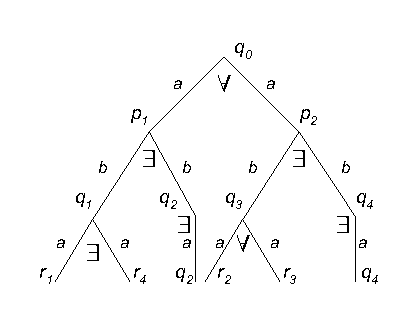
\includegraphics{img/afsa_aka}
  \caption{Úplný strom konfigurácií AFSA $A$ na slove $w=aba$}
  \label{afsa_aka}
\end{figure}

\section{Alternujúce zásobníkové automaty ($APDA$)}

Ako sme ukázali, konečným automatom alternovanie v generatívnej
sile vôbec nepomohlo. Lepšia je situácia v oblasti bezkontextových
jazykov, ktoré rozpoznávajú zásobníkové automaty (PDA). Tu
alternovanie zvýši možnosť rozpoznávania jazykov až na úroveň, o
ktorej hovorí nasledujúce tvrdenie

\begin{veta}\label{apda}
  $\underset{c}{\bigcup} DTIME(c^n)\subseteq\mathcal{L}_{APDA}$
\end{veta}

\begin{dokaz}
  Tvrdenie nebudeme dokazovať priamo, využijeme tvrdenie vety
  \ref{dtime_aspace}, podľa ktorého platí $\underset{c}{\bigcup}
  DTIME(c^n)\subseteq ASPACE(n)$. My ukážeme, že platí
  $ASPACE(n)\subseteq\mathcal{L}_{APDA}$, potom bude z tranzitívnosti
  relácie $\subseteq$ platiť aj
  $\underset{c}{\bigcup}DTIME(c^n)\subseteq\mathcal{L}_{APDA}$.

  \smallskip
  Na dôkaz $ASPACE(n)\subseteq\mathcal{L}_{APDA}$ potrebujeme k
  ATS $A$, ktorý pre vstup dĺžky $n$ používa $n$ políčok na
  pracovnej páske, zostrojiť APDA $A'$ taký, že
  $L(A)=L(A')$. Bez újmy na všeobecnosti budeme predpokladať, že
  úplný strom konfigurácií $A$ je binárny\footnote{čitateľ si
  iste vie predstaviť podobnú konštrukciu ako v leme
  \ref{binarny_nt2} pre APDA}.

  \smallskip
  $A'$ bude pracovať nasledovne\footnote{idea je nasledovná: v
  zásobníku bude simulovať výpočet ATS $A$ tak, že do neho bude
  postupne pridávať konfigurácie $A$ a overovať ich náväznosť
  vzhľadom na $\vdash$, keď pridá do zásobníka akceptačnú
  konfiguráciu, ktorá bude nadväzovať na predchádzajúce, akceptuje}:
  \begin{itemize}
    \item najskôr v existenčnom vetvení uhádne počiatočnú
    konfiguráciu (bude hádať $n+1$ symbolov, háda aj stav) $q_0w$,
    pričom $w=a_1\dots a_n$, v obrátenom poradí, teda zásobník bude
    mať po $n+1$ krokoch tvar ako na (obr.\ref{zasobnik1}a)
    \item v univerzálnom vetvení v jednej vetve overí, či konfiguráciu
    hádal správne, v druhej vetve háda nasledovníkov konfigurácie
    $q_0w$ vo vetvení, ktorého typ zodpovedá vetveniu v úplnom strome
    konfigurácií $A$, každej konfigurácii priradí aj vetvu, v ktorej
    sa nachádzala v úplnom strome konfigurácií $A$ (teda L,R),
    konfigurácie ďalej overí a háda ďaľšie, až kým neakceptuje, resp.
    neodmietne (REJECT) vstup
    \item do overenia, či konfigurácie na seba nadväzujú, spadá:
      \begin{itemize}
        \item overiť, či sme hádali správnu vetvu (prvky $\delta_A$
        si usporiadame L,R)
        \item $A'$ musí po jednotlivých symboloch prejsť konfigurácie a
        testovať ich na rovnosť (obr.\ref{zasobnik1}b), resp. možnosť
        prechodu v $\delta_A$, univerzálne sa rozvetví: v jednej vetve
        overí, či sa 1. symbol zhoduje s ($n+k$)-tym symbolom\footnote{$k$
        je konštanta, jej určenie prenechávame na čitateľa}, resp.či
        existuje v $\delta_A$ prechod taký, aby sa symboly na seba mohli
        prepísať, tak, že zo zásobníka zmaže $n+k$ symbolov (je dôležité
        uvedomiť si, že do tejto chvíle sme v tejto vetve vstup nečítali,
        tu ho používame na počítanie $n$, zrejme bude dobre vždy si v
        stave pamätať 4 symboly z vrchu pôvodného obsahu zásobníka pred
        vymazávaním), v ďaľšej overí, či 2. až ($n+1$)-vý symbol z prvej
        konfigurácie sedí podľa $\delta_A$ s 2. až ($n+1$)-vým symbolom
        druhej konfigurácie podobne ako pre 1. symbol
      \end{itemize}
  \end{itemize}
  Čitateľovi odporúčame podrobnejšie rozpracovať overovanie
  konfigurácii, najmä overenie, či sa konfigurácia nachádzala v
  ľavej, alebo pravej vetve vzhľadom na svojho predka, v úplnom
  strome konfigurácií ATS $A$. Na pochopenie, že $L(A)=L(A')$ by
  však úroveň detailu v našej konštrukcii mala byť dostačujúca
\end{dokaz}

\begin{figure}[!ht]
  \centering
  \includegraphics{img/zasobnik1}
  \caption{Zásobník APDA $A'$ a) po uhádnutí $q_0w$ b) pri overovaní
  náväznosti konfigurácií} \label{zasobnik1}
\end{figure}

\begin{poznamka}
  Platí aj obrátená inklúzia, jej dôkaz však presahuje rozsah tohto
  textu, navyše na ukážku, že alternovanie zásobníkovým automatom
  pomáha v generatívnej sile, stačí veta \ref{apda}
\end{poznamka}

\section{Synchronizované alternujúce stroje}

Ukážeme si jednu modifikáciu pôvodného modelu alternujúcich strojov,
keď umožníme jed\-no\-du\-chú komunikáciu medzi paralelnými procesmi.
Zavedieme nové delenie stavov alternujúceho
stroja, nezávisle od delenia na existenčné a univerzálne stavy,
na:
\begin{itemize}
  \item obyčajné
  \item synchronizačné - dvojica $(q,S)\ra($stav,symbol$)$
\end{itemize}
Keď proces prejde do synchronizačného stavu, čaká, kým všetky
ostatné prejdu do synchronizačného stavu. Keď majú všetky rovnaký
symbol v druhej komponente synchronizačného stavu, pokračujú,inak
sa zariadenie zablokuje

\begin{priklad}
  Ukážeme si, že keď umožníme synchronizáciu konečným automatom, tak
  sa nám ich podarí posunúť z triedy regulárnych jazykov. Na
  (obr.\ref{anbnc}) je znázornený synchronizovaný konečný automat,
  ktorý akceptuje bezkontextový jazyk $L=\{a^nb^nc\mm n\geq1\}$
\end{priklad}

\begin{figure}[!ht]
  \centering
  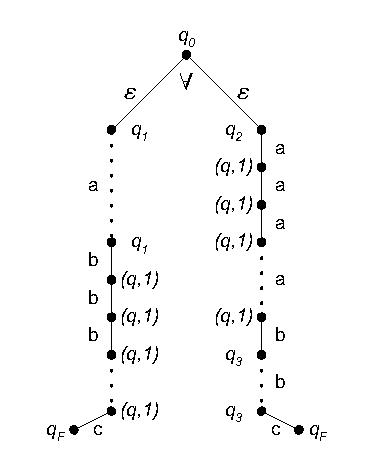
\includegraphics{img/anbnc}
  \caption{Synchronizovaný konečný automat pre jazyk $L=\{a^nb^nc\mm
  n\geq1\}$} \label{anbnc}
\end{figure}

\begin{poznamka}
  Dá sa ukázať tvrdenie, ktoré hovorí o tom, že trieda jazykov
  rozpoznávaných synchronizovanými konečnými automatmi je presne
  $\Langclass{CS}$
\end{poznamka}

\chapter{Booleovské obvody ($BO$)}

\section{Definície a označenia}

\begin{definicia}
Booleovský obvod $(BO)$ je konečný acyklický orientovaný graf, v
ktorom každému vrcholu $v$ priradíme typ $\tau (v)\in \{
B_{IN}\}\cup\{ B_0\}\cup\{ B_1\}\cup\{ B_2\}$ a hodnotu
$\mathcal{V}(v)\in\{ 0,1\}$. Vrchol $v$, pre ktorý typ $\tau
(v)\in\{ B_{IN}\}$, má vstupný stupeň 0 a nazývame ho vstupný
vrchol. Vstupom pre booleovský obvod je $n$-tica rôznych vstupných
vrcholov označených $\langle x_1,\dots ,x_n\rangle$. Vrchol $v$,
pre ktorý typ $\tau (v)\in\{ B_i\}$, má vstupný stupeň $i$ a
nazývame ho hradlo. Medzi hradlá typu $B_0$ patria konštanty ``0''
a ``1'', do $B_1$ patria hradlá ``$I$'' a ``$\neg$''
reprezentujúce booleovské funkcie identita a negácia a do $B_2$
patria hradlá ``$\wedge$'' a ``$\vee$'' reprezentujúce booleovské
funkcie AND a OR. Vrcholy s výstupným stupňom 0 nazývame výstupné.
Výstupom pre booleovský obvod je $m$-tica rôznych výstupných
vrcholov označených $\langle y_1,\dots ,y_m\rangle$.
\end{definicia}

\begin{definicia}
Booleovský obvod so vstupom $\langle x_1,\dots ,x_n\rangle$ a
výstupom $\langle y_1,\dots ,y_m\rangle$ počíta\linebreak funkciu
$f:\;\{ 0,1\}^n\rightarrow \{ 0,1\}^m$ nasledovne. Každý vstupný
vrchol $x_i$ má danú hodnotu\linebreak $\mathcal{V}(x_i)\in\{
0,1\}$. Každé hradlo $h$ jednoznačne vyhodnotí hodnotu
$\mathcal{V}(h)$ aplikovaním elementárnej booleovskej funkcie
$\tau (h)$ na hodnoty vstupných vrcholov. Výsledná hodnota funkcie
$f$ je daná $m$-ticou hodnôt výstupných vrcholov $\langle
\mathcal{V}(y_1),\dots ,\mathcal{V}(y_m)\rangle$.
\end{definicia}

Všimnime si, že v definícii sme ohraničili počet vstupov vrchola,
ale nie počet výstupov. Takisto sme nezakázali, aby vstupný vrchol
bol zároveň výstupným.

Ak chceme pomocou modelu $BO$ definovať jazyky, je rozumné sa
obmedziť na $BO$ s jedným výstupným vrcholom, pričom slovo na
vstupe z $\{ 0,1\}^*$ akceptujeme práve vtedy, keď hodnota
výstupného vrchola bude 1. Toto so sebou prináša jednu
nepríjemnosť, pretože $BO$ má konečný počet vstupných vrcholov, a
teda je schopný akceptovať len konečné jazyky. Preto jazyky budeme
definovať pomocou triedy booleovských obvodov.

\begin{definicia}
Nech $\{C_n\}_{n=0}^{\infty}$ je postupnosť booleovských obvodov,
kde $BO$ $C_n$ s $n$ vstupnými a $m(n)$ výstupnými vrcholmi počíta
funkciu $f_n:\; \{ 0,1\}^n\rightarrow\{ 0,1 \}^{m(n)}$. Túto
postupnosť nazývame trieda booleovských obvodov $\{ C_n\}$
počítajúca funkciu $f:\; \{ 0,1\}^*\rightarrow\{ 0,1\}^*$
definovanú takto: $f(w)\equiv f_n(w)$ práve vtedy, keď $|w|=n$.
\end{definicia}

\begin{definicia}
Nech $\{ C_n\}$ je trieda (postupnosť) booleovských obvodov
počítajúca funkciu \\ $f:\; \{ 0,1\}^*\rightarrow\{ 0,1\}$, teda
každý $BO$ má jeden výstupný vrchol. Jazyk akceptovaný triedou $\{
C_n\}$ definujeme takto: $L(\{ C_n\})=\{ w\in\{ 0,1\}\mm
f(w)=1\}$.
\end{definicia}

\section{Miery zložitosti}

Pre booleovské obvody definujeme nasledujúce miery zložitosti:
\begin{itemize}
  \item $DEPTH(C_n)$ = dĺžka najdlhšej cesty v obvode $C_n$
  \item $SIZE(C_n)$ = počet hradiel obvodu $C_n$
\end{itemize}

Ak predpokladáme, že čas, ktorý potrebuje hradlo na vyhodnotenie
výstupu je jedna časová jednotka, a čas potrebný na prenos
informácie medzi hradlami neuvažujeme, potom miera $DEPTH$ je
ekvivalentná časovej náročnosti výpočtu na $BO$.

\begin{priklad}
Chceme vypočítať skalárny súčin dvoch $n$-bitových vektorov
$(x_1,\dots ,x_n)$ a \linebreak $(y_1,\dots ,y_n)$. Vieme, že ich
skalárny súčin vypočítame takto: $(x_1\wedge y_1)\vee\dots\vee
(x_n\wedge y_n)$. \linebreak Príslušný $BO$ realizujúci tento
výpočet je znázornený na obrázku \ref{bo_obr_scalsuc}a, z ktorého ľahko \linebreak
vidieť, že $SIZE(C_n)=2n-1=O(n)$ a $DEPTH(C_n)=n=O(n)$.
\end{priklad}

\begin{priklad}
\label{bo_prikl_2}

Opäť chceme vypočítať skalárny súčin dvoch $n$-bitových vektorov,
tentoraz však použijeme iný $BO$ $C_n$ (obr. \ref{bo_obr_scalsuc}b). Pri
zachovaní rovnakého počtu hradiel sme znížili hĺbku obvodu na
$DEPTH(C_n)=O(\log n)$.
\end{priklad}

\begin{figure}[!ht]
  \centering
  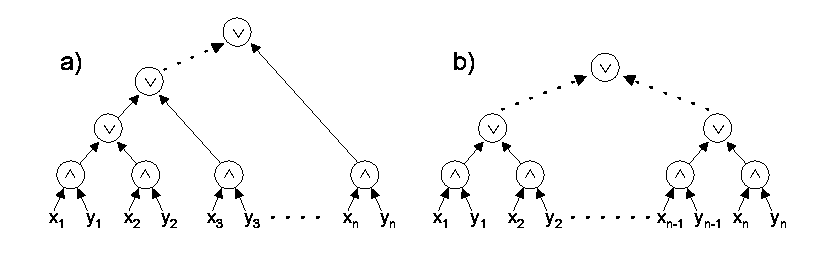
\includegraphics{img/bo/scalsuc}
  \caption{Výpočet skalárneho súčinu na $BO$} \label{bo_obr_scalsuc}
\end{figure}

\begin{priklad}
\label{bo_prikl_3}

Chceme vynásobiť dve booleovské matice $A$ a $B$ rozmeru $n\times
n$. Výsledok je matica rovnakého rozmeru $C$, pričom jej prvky
vypočítame nasledovne: $c_{i,j}=\bigvee\limits_{k=1}^{n}
a_{ik}\wedge b_{kj}$. To je $n^2$ nezávislých skalárnych súčinov.
Ak budeme každý takýto súčin počítať podľa príkadu
\ref{bo_prikl_2} dostaneme príslušný obvod $C_n$, pre ktorý platí,
že $SIZE(C_n)=O(n^3)$ a $DEPTH(C_n)=O(\log)$.
\end{priklad}

\begin{priklad}
\label{bo_prikl_4}

Teraz sa pokúsime vyrobiť reflexívny a tranzitívny uzáver
booleovskej matice $M$ rozmeru $n\times n$. Výsledkom je matica
$M^*$, ktorú dostaneme nasledovným výpočtom: \\ $M^*=I\vee M\vee
M^2\vee\dots M^n$, kde $M^i=\bigwedge\limits_{k=1}^{i} M$, čo
znamená, že $M^*=(I\vee M)^n$. Ak na výpočet súčinu matíc
použijeme obvod z príkladu \ref{bo_prikl_3} a štruktúru úplného
binárneho stromu (obr. \ref{bo_obr_tranzuzm}) dostaneme obvod $C_n$ počítajúci
$M^*$, pre ktorý platí $SIZE(C_n)=O(n^4)$ a $DEPTH(C_n)=O(\log^2
n)$.
\end{priklad}

\begin{figure}[!ht]
  \centering
  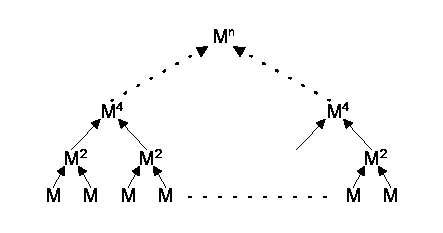
\includegraphics{img/bo/tranzuzm}
  \caption{Výpočet reflexívneho a tranzitívneho uzáveru matice} \label{bo_obr_tranzuzm}
\end{figure}

\section{$BC$-uniformné booleovské obvody}

Postupnosť booleovských obvodov, ako neskôr uvidíme, dokáže
akceptovať triedu jazykov $\mathcal{L}_{RE}$, ale tak ako sme ju
zatial zadefinovali dokáže akceptovať ešte viac, pretože
postupnosť $BO$ môžeme určiť tak, že pre rôzne dĺžky vstupu bude
používať úplne iný mechanizmus spracovania vstupného slova, čo v
iných modeloch v zásade nie je možné. Preto doterajší model $BO$
trochu zoslabíme zavedením akejsi ``pravidelnosti'' (uniformity)
do postupnosti $BO$.

\begin{definicia}
Postupnosť booleovských obvodov je uniformná, ak existuje nejaký
deterministický stroj ($DTS$, $ATS$), ktorý na vstupe $1^n$
vygeneruje $BO$ $C_n$ resp. jeho kód.
\end{definicia}

\begin{definicia}
(Štandardný kód $BO$)
\\ Kód booleovského obvodu $C_n$ (ozn. $\langle C_n\rangle$) je postupnosť
štvoríc $\langle g,t,a,b\rangle$, kde $g\in\{ 0,1\}^+$ je
jednoznačné číslo vrchola, $t\in\{ 0, 1, I,\neg,\wedge,\vee, x\}$
je typ vrchola $g$ ($x$ označuje vstup),\newline $a,b\in\{
0,1\}^+$ sú čísla ľavého a pravého vstupu vrchola $g$. Vstupným
vrcholom $x_1,\dots ,x_n$\linebreak štandardne priradíme čísla
$1,\dots ,n$ a výstupnému vrcholu (ak je len jeden) priradíme
číslo 0.
\end{definicia}

\begin{definicia}
Postupnosť booleovských obvodov $\{ C_n\}$ je $BC$-uniformná
($BC$-uniformne \linebreak konštruovateľná\footnote{$BC$ -
Borodin, Cook}), ak existuje $DTS$, ktorý pre každé $n$ na vstupe
$1^n$ vygeneruje kód booleovského obvodu $\langle C_n\rangle$ v
priestore\footnote{všimnime si, že pracovný priestor neurčujeme podľa veľkosti
vstupu, ale na základe veľkosti vygenerovaného výstupu} $\log
(SIZE(C_n))$.
\end{definicia}

\begin{figure}[!ht]
  \centering
  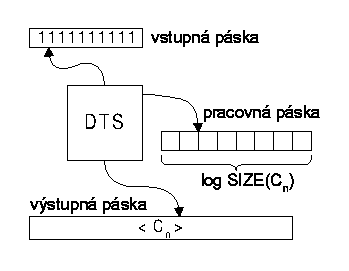
\includegraphics{img/bo/ubcdts}
  \caption{$DTS$ generujúci kód booleovského obvodu} \label{bo_obr_ubcdts}
\end{figure}

Čísla vrcholov v kóde obvodu $C_n$ kódujeme binárne, takže pre
veľkosť kódu dostávame\linebreak {$|\langle C_n\rangle|=O(SIZE(C_n).\log
SIZE(C_n))$, čo nám určuje časovú zložitosť $DTS$ z definície\linebreak
$BC$-uniformity.\\ Ďalším predpokladom na tento $DTS$ je
topologické usporiadanie výstupu t.j. kód vrchola $C_n$ sa na
výstupe neobjaví skôr ako kódy jeho vstupov.

\begin{poznamka}\label{bo_pozn_bcuniformita}
$BC$-uniformita zabezpečuje len to, aby sme s jazykmi nevyšli z
triedy $\mathcal{L}_{RE}$, teda v návrhoch postupností $BO$ nás
príliš neobmedzuje. Preto aj každá ``rozumne'' navrhnutá
postupnosť $BO$ je $BC$-uniformná.
\end{poznamka}

\begin{oznacenie}
$\mathcal{U}_{BC}DEPTHSIZE(D(n),S(n))$ - trieda jazykov. Pre každý
jazyk z tejto triedy existuje $BC$-uniformná postupnosť
booleovských obvodov $\{ C_n\}$ akceptujúca daný jazyk pričom
$DEPTH(C_n)=O(D(n))$ a $SIZE(C_n)=O(S(n))$.
\end{oznacenie}

\section{Porovnanie $BO$ a $TS$}

\begin{veta}
\label{bo_veta_dtimetobosize}

Ak $L$ je jazyk akceptovaný jednopáskovým $DTS$ v čase $T(n)$,
potom existuje \linebreak $BC$-uniformná postupnosť $BO$ $\{
C_n\}$ taká, že $L(\{ C_n\})=L$ a $SIZE(C_n)=O(T^2(n))$.
\end{veta}

\begin{dokaz}
Uvažujme $DTS\; A$ a jazyk $L$ zo znenia vety. Zoberme si nejaké
slovo $w=a_1\dots a_n\in L$. Ukážeme si ako bude vyzerať $BO$
$C_n$ akceptujúci slová dĺžky $n$ z jazyka $L$.

Najskôr binárne zakódujeme všetky symboly vstupnej a pracovnej
abecedy a všetky stavy $DTS\; A$ t.j. všetkým jednoznačne
priradíme nenulový binárny vektor. Obvod $C_n$ bude mať $T(n)$
úrovní, pričom na $i$-tej úrovni bude ``udržiavať'' informáciu o
$i$-tej konfigurácii $A$ pri výpočte na slove $w$ nasledovným
spôsobom. Každá úroveň bude pozostávať z elementárnych obvodov
$(eBO)$ reprezentujúcich jedno políčko pracovnej pásky $A$, pričom
jeden takýto obvod dostane na vstup kód znaku, ktorý je na danom
políčku, a kód stavu, v ktorom je $A$, ak sa hlava $A$ nachádza na
tomto políčku (obr. \ref{bo_obr_tsboebo}a).

Z mechanizmu výpočtu Turingovho stroja vieme, že zmeny
konfigurácií sú len lokálneho charakteru t.j. v jednom kroku
výpočtu sa môže zmeniť len jednopísmenkové okolie pozície hlavy.
Podobne aj v našom obvode $C_n$ jeden elementárny obvod môže
ovplyvniť len svojho nasledovníka a jeho susedov, preto sú
jednotlivé elementárne obvody pospájané ako na obrázku \ref{bo_obr_tsboebo}b.

\begin{figure}[!ht]
  \centering
  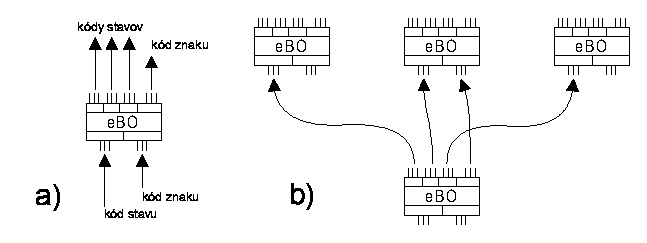
\includegraphics{img/bo/tsboebo}
  \caption{Elementárny booleovský obvod $(eBO)$} \label{bo_obr_tsboebo}
\end{figure}

Každý elementárny obvod bude pracovať nasledovne:
\begin{enumerate}
  \item ak na vstup dostane kód nejakého znaku a nulový vektor ako
  kód stavu, znamená to, že hlava $A$ nie je na políčku, ktoré je
  reprezentované týmto obvodom a na výstup pošle kód prijatého znaku
  a nulový vektor ako kód stavu (obr. \ref{bo_obr_tsbo2}a)
  \item ak na vstup dostane kód znaku $a$ a kód stavu $q$, tak
  podľa definície $\delta$-funkcie $A$ pošle na výstup kód nového
  znaku $b$, a podľa pohybu hlavy v $\delta$-funkcii pošle
  príslušnému obvodu v nasledujúcej úrovni kód nového stavu, čím
  ho informuje o tom, že v nasledujúcom kroku bude hlava nad jeho
  políčkom a  ostatným dvom pošle ako kód stavu nulový vektor
  (\mbox{obr. \ref{bo_obr_tsbo2}b} pre $\delta$-funkciu $DTS$, ktorá pošle hlavu vľavo)
\end{enumerate}

\begin{figure}[!ht]
  \centering
  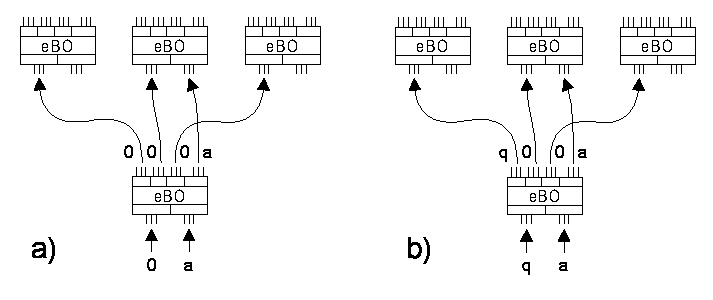
\includegraphics{img/bo/tsbo2}
  \caption{Komunikácia medzi úrovňami $eBO$} \label{bo_obr_tsbo2}
\end{figure}

Takže celý obvod $C_n$ bude mať $T^2(n)$ elementárnych obvodov
($T(n)$ úrovní pre každú kon\-fi\-gu\-rá\-ciu a v každej úrovni
$T(n)$ obvodov pre každé políčko\footnote{v každej úrovni by
stačilo $S(n)$ (veľkosť pracovného priestoru) obvodov, ale nemáme
žiaden predpoklad na priestor $DTS\; A$, vieme však, že určite
platí $S(n)\leq T(n)$ }). Vstupom pre $C_n$ bude počiatočná
konfigurácia $A$, teda prvý obvod v prvej úrovni dostane na vstup
kód počiatočného stavu a kód prvého písmenka slova $w=a_1\dots
a_n$, ďalších $n-1$ obvodov dostane na vstup kódy zvyšných $n-1$
písmenok slova $w$ a nulové vektory ako kódy stavov, a ostatné
obvody dostanú na \mbox{vstup} nulové vektory ako kódy znakov aj
stavov (obr. \ref{bo_obr_tsbo3}). Ďalej bude každý elementárny obvod pracovať
ako sme už uviedli, takže jednotlivé úrovne obvodu $C_n$ budú krok
po kroku zodpovedať konfiguráciám vo výpočte $A$. Na úrovni $T(n)$
už iba skontrolujeme, či nejaký $eBO$ je v akceptačnom stave, ak
áno, na výstup dáme jednotku inak nulu.

\begin{figure}[!ht]
  \centering
  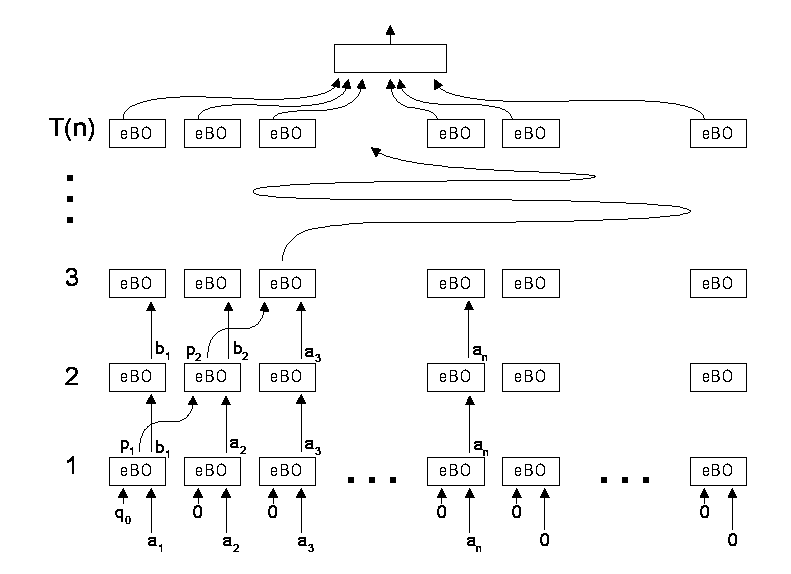
\includegraphics{img/bo/tsbo3}
  \caption{Simulácia $DTS$ booleovským obvodom} \label{bo_obr_tsbo3}
\end{figure}

Z uvedeného vyplýva, že $DEPTH(C_n)=T(n)$, a keďže uvažujeme
konečný počet stavov, symbolov abecedy a konečný zápis
$\delta$-funkcie $DTS\; A$, tak dokážeme realizovať elementárny
obvod z konečného počtu hradiel, z čoho nakoniec plynie, že
$SIZE(C_n)=O(T^2(n))$.

Týmto sme ukázali, že $L\subseteq L(\{ C_n\})$. Opačná inklúzia
(t.j. že takto zostrojená postupnosť $BO$ neakceptuje žiadne slovo
mimo jazyka $L$) je z konštrukcie zrejmá.

To, že takto vytvorená postupnosť $BO$ je naozaj $BC$-uniformná,
nebudeme formálne dokazovať. Obmedzíme sa len na fakt, že každý
obvod $C_n$ tejto postupnosti bude vytváraný rovnakým postupom, čo
v súlade s poznámnkou \ref{bo_pozn_bcuniformita} zabezpečuje
$BC$-unifomitu.
\end{dokaz}

\begin{veta}
\label{bo_veta_bosizetodtime}

Ak $L$ je jazyk akceptovaný $BC$-uniformnou postupnosťou $BO$ $\{
C_n\}$, pričom\linebreak $SIZE(C_n)=S(n)$, potom existuje $DTS$
akceptujúci jazyk $L$ v čase $S^3(n)$.
\end{veta}

\begin{dokaz}
Nech $\{ C_n\}$ je postupnosť $BO$ zo znenia vety. Chceme
zozstrojiť $DTS\; A$ taký, že $L(A)=L$. Postupnosť $\{ C_n\}$ je
$BC$-uniformná, teda poznáme $DTS\; A'$, ktorý vygeneruje kód
$\langle C_n\rangle$. $DTS\; A$ bude na vstupnom slove $w$ dĺžky
$n$ pracovať nasledovne:
\begin{enumerate}
  \item $A$ si na pásku napíše kód $BO$ $C_n$ simulovaním $A'$
  so vstupom\footnote{Takýto vstup máme k dispozícii zo vstupného
  slova $w$ tým, že všetky symboly budeme považovať za 1.} $1^n$.
  To dokáže v čase $O(S(n).\log S(n))$, lebo kód
  $\langle C_n\rangle$ je takejto dĺžky.
  \item $A$ bude postupne ohodnocovať\footnote{ohodnotiť hradlo
  znamená na páske označiť symboly príslušného hradla v kóde $C_n$
  hodnotami 0 alebo 1}
  vrcholy $BO$ $C_n$ tak, že vstupné vrcholy ohodnotí podľa
  príslušných hodnôt vstupu a hradlá ohodnotí podľa hodnôt vstupov
  hradla a jeho typu. Ohodnocovanie musí samozrejme prebiehať v topologickom
  usporiadaní. Na ohodnotenie jedného vrchola potrebuje $A$ v
  najhoršom prípade prejsť celú pásku trikrát (dvakrát na nájdenie
  hodnôt vstupov a tretí krát na nájdenie a ohodnotenie samotného
  vrchola). Vrcholov je $S(n)$, veľkosť pásky je $O(S(n).\log S(n))$,
  teda na ohodnotenie všetkých vrcholov $C_n$ potrebuje $A$ čas
  $O(S^2(n).\log S(n))$.
\end{enumerate}
$A$ akceptuje vstupné slovo práve vtedy, keď výstupný vrchol
ohodnotí jednotkou. Teda ukázali sme, že $L\subseteq L(A)$. Opačná
inklúzia je z konštrukcie zrejmá. Obidva kroky výpočtu vykoná $A$
v čase $O(S^2(n).\log S(n))$, čo je samozrejme v $O(S^3(n))$.
\end{dokaz}

\begin{dosledok}
$DTIME(Poly)=\mathcal{U}_{BC} SIZE(Poly)$
\end{dosledok}

\begin{dokaz}
Z vety \ref{bo_veta_dtimetobosize} sme dostali
$DTIME(T(n))\subseteq\mathcal{U}_{BC} SIZE(T^2(n))$.

Z vety \ref{bo_veta_bosizetodtime} sme dostali $\mathcal{U}_{BC}
SIZE(S(n))\subseteq DTIME(S^3(n))$.

Spojením týchto výsledkov teda dostávame
$DTIME(Poly)=\mathcal{U}_{BC} SIZE(Poly)$. To znamená, že vo
výpočtovom modeli $BO$ vieme polynomiálny sekvenčný čas premieňať
na polynomiálny paralelný priestor a opačne.
\end{dokaz}

\begin{veta}
\label{bo_veta_nspacetobodepth}

Ak $L$ je jazyk akceptovaný $NTS$, pracujúcim s jednou vstupnou a
jednou pracovnou páskou, v priestore $S(n)\geq\log n$, potom
existuje $BC$-uniformná postupnosť $BO$ $\{ C_n\}$ taká, že $L(\{
C_n\})=L$ a $DEPTH(C_n)=O(S^2(n))$.
\end{veta}

\begin{dokaz}
Uvažujme jazyk $L$ a $NTS\; A$ zo znenia vety. Zostrojíme $BO$
$C_n$ akceptujúci slová dĺžky $n$ z jazyka $L$. Zoberme si nejaké
slovo $w\in L$, kde $|w|=n$. Zamyslime sa nad tým v koľkých
možných konfiguráciach môže byť $A$ počas výpočtu na vstupnom
slove $w$. Ak berieme do úvahy počty stavov, symbolov abecedy,
políčok pracovnej pásky, možné pozície hlavy na vstupnej a
pracovnej páske, dostaneme, že počet všetkých možných konfigurácií
je $k^{S(n)}$ pre vhodnú konštantu $k$.

Uvažujme ďalej reláciu krok výpočtu $\vdash$ na týchto
konfiguráciach. Za predpokladu, že binárne zakódujeme stavy a
symboly abecedy, dokážeme reláciu $\vdash$ reprezentovať
booleovskou maticou rozmeru $k^{S(n)}\times k^{S(n)}$, čo je pre
pevne stanovené $n$ konečná matica. Predpokladajme, že $A$ má
jednoznačne danú akceptačnú konfiguráciu. Potom otázka, či vstupné
slovo $w$ patrí do jazyka $L$, je vlastne otázka, či počiatočná
konfigurácia $A$ je v relácii $\overset{*}{\vdash}$ s akceptačnou
konfiguráciou. Relácia $\overset{*}{\vdash}$ je reflexívnym a
tranzitívnym uzáverom relácie $\vdash$. Keďže túto reláciu vieme
reprezentovať konečnou booleovskou maticou, z príkladu
\ref{bo_prikl_4} plynie, že aj reláciu $\overset{*}{\vdash}$ vieme
reprezentovať konečnou booleovskou maticou, ktorú dostaneme
konečným násobením mocnín matice reprezentujúcej reláciu $\vdash$.
Z uvedeného príkladu tiež vieme, že reflexívny a tranzitívny
uzáver booleovskej matice $M$ rozmeru $k^{S(n)}\times k^{S(n)}$
vypočítame na $BO$ hĺbky rádovo $\log^2 k^{S(n)}=O(S^2(n))$.

Teda náš $BO$ $C_n$ so vstupom $\langle w\rangle$ najskôr zostrojí
maticu relácie $\vdash$ na vstupnom slove $w$ (to sa dá konečným
$BO$, v ktorom je zakódovaná $\delta$-funkcia $A$), a potom už
spomínaným spôsobom urobí nad touto maticou jej reflexívny a
tranzitívny uzáver. $A$ akceptuje práve vtedy, keď vo výslednej
matici je na i-tom riadku a j-tom stĺpci 1, kde i-ty riadok
reprezentuje počiatočnú konfiguráciu a j-ty stĺpec reprezentuje
akceptačnú konfiguráciu. Takto sme ukázali, že $L\subseteq L(\{
C_n\})$, pričom $DEPTH(C_n)=O(S^2(n))$. Opačná inklúzia je z
konštrukcie zrejmá.

Tvrdenie o tom, že vytvorená postupnosť $BO$ je $BC$-uniformná,
nechávame opäť na poznámku \ref{bo_pozn_bcuniformita}.
\end{dokaz}

\begin{veta}
\label{bo_veta_bodepthtodspace}

Ak $L$ je jazyk akceptovaný $BC$-uniformnou postupnosťou $BO$ $\{
C_n\}$, pričom\linebreak $DEPTH(C_n)=D(n)$, potom existuje $DTS$
akceptujúci jazyk $L$ v priestore $O(D(n))$.
\end{veta}

\begin{dokaz}
Uvažujme jazyk $L$ a postupnosť $BO$ $\{ C_n\}$ zo znenia vety.
Chceme zostrojiť príslušný $DTS\;A$. Nech $w\in L$ je dĺžky $n$, čiže
kód $\langle w\rangle$ je akceptovaný $BO$ $C_n$ z postupnosti $\{
C_n\}$. Vieme, že $\{ C_n\}$ je $BC$-uniformná, takže existuje
generátor $A'$ kódu $\langle C_n\rangle$ pracujúci v priestore
$\log (SIZE(C_n))$. Zrejme $\log (SIZE(C_n))\in O(D(n))$, takže $A$ má
dostatok priestoru, aby mohol simulovať $A'$, ale nemá dosť
priestoru na uloženie celého kódu $\langle C_n\rangle$. Nemôžeme
teda použiť techniku ohodnocovania $C_n$ ako v dôkaze vety
\ref{bo_veta_bosizetodtime}.

$A$ bude postupne ohodnocovať vrcholy $C_n$ postorder
prehľadávaním $C_n$ od výstupného vrcholu (vstupný vrchol ohodnotí
podľa príslušnej časti vstupu $\langle w\rangle$ a vnútorný podľa
hodnôt jeho\linebreak vstupov). $A$ však nemá na páske ani toľko
priestoru, aby si zapamätal kódy všetkých vrcholov na ceste od
výstupného k práve prehľadávanému vrcholu\footnote{Cesta môže byť
dlhá maximálne $D(n)$ a kód každého vrcholu je veľkosti rádovo
$\log SIZE(C_n)$, takže by sme potrebovali priestor rádovo $D^2(n)$.}. Preto
si bude na páske pamätať len navigačnú cestu od výstupného k práve
prehľadávanému vrcholu (obr. \ref{bo_obr_bots}). Ak sa chce $A$ posunúť pri
prehľadávaní z jedného vrchola do druhého (t.j. z otca do syna
alebo opačne), zakaždým musí spustiť simuláciu $A'$ a v jeho
výstupe nájsť kód príslušného vrchola. Vstupné slovo $w$ bude $A$
akceptovať práve vtedy, keď výstupný vrchol dostane hodnotu 1.

\begin{figure}[!ht]
  \centering
  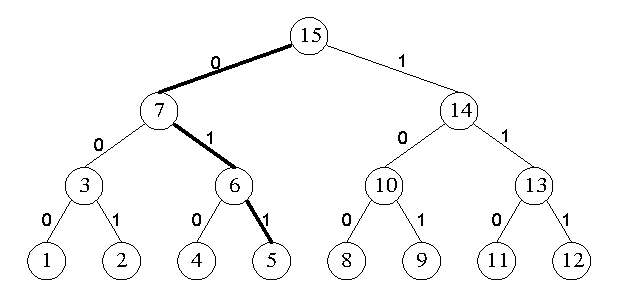
\includegraphics{img/bo/bots}
  \caption{Postorder prehľadávanie booleovského obvodu} \label{bo_obr_bots}
\end{figure}

Takže $A$ si bude na páske udržiavať kódy práve prehľadávaného
vrcholu a niekoľko málo vrcholov v jeho okolí (aby mohol vrchol
ohodnotiť), navigačnú cestu od koreňa k prehľadávanému vrcholu a
už známe ohodnotenia vrcholov, ktoré má aktuálne na páske. Na toto
potrebuje $A$ priestor rádovo $D(n)$. Na simulovanie $A'$
potrebuje tiež priestor rádovo $D(n)$, takže veľkosť pracovnej
pásky $A$ bude $O(D(n))$.

Týmto sme ukázali, že $L\subseteq L(A)$, opačná inklúzia by opäť
mala byť z konštrukcie zrejmá.
\end{dokaz}

\pagebreak

\begin{dosledok} \label{bo_dosl_nspacepolyubcdepthpoly}
$NSPACE(Poly)=\mathcal{U}_{BC} DEPTH(Poly)$
\end{dosledok}

\begin{dokaz}
Z vety \ref{bo_veta_nspacetobodepth} sme dostali
$NSPACE(S(n))\subseteq\mathcal{U}_{BC} DEPTH(S^2(n))$.

Z vety \ref{bo_veta_bodepthtodspace} sme dostali $\mathcal{U}_{BC}
DEPTH(D(n))\subseteq DSPACE(D(n))$.

Zo Savitchovej vety vieme, že $DSPACE(Poly)=NSPACE(Poly)$.

Spojením týchto výsledkov teda dostávame
$NSPACE(Poly)=\mathcal{U}_{BC} DEPTH(Poly)$. To\linebreak znamená,
že vo výpočtovom modeli $BO$ vieme polynomiálny sekvenčný priestor
premieňať na polynomiálny paralelný čas a opačne.
\end{dokaz}


\section{Druhá počítačová trieda a Nick Class}

V tejto časti si povieme nakoľko sú paralelné výpočtové modely, ktoré sme doteraz spomenuli a ktoré
ešte len spomenieme, vhodné na efektívne riešenie problémov, či je daný model vhodne zadefinovaný a
ukážeme si akými mierami budeme posudzovať vhodnosť daného modelu.

\begin{definicia}
Model počítača patrí do druhej počítačovej triedy, ak sekvenčný nedeterministický
priestor je v polynomiálnom vzťahu s časom na danom modeli.
\end{definicia}

Predchádzajúca definícia hovorí o tom aké kritérium sme zvolili na posudzovanie toho, či je nejaký
výpočtový model pre nás zaujímavý (vhodný). Z doteraz spomenutých modelov patria do druhej
počítačovej triedy modely Alternujúcich Turingových strojov (dôsledok
\ref{alter_dosl_nspacepolyatimepoly}) a $BC$-uniformných booleovských obvodov (dôsledok
\ref{bo_dosl_nspacepolyubcdepthpoly}).

Takmer všetky paralelné modely patria do druhej počítačovej triedy. Ak uvažujeme nejaký nový model
a chceme ho zaradiť do druhej počítačovej triedy, tak môžme urobiť simuláciu daného modelu s
Turingovým strojom podobne, ako sme to urobili vo vetách \ref{bo_veta_nspacetobodepth} a
\ref{bo_veta_bodepthtodspace}, alebo urobíme simuláciu s modelom, ktorý tam už patrí.

Ďalšou otázkou, ktorá je pre nás zaujímavá, je aké problémy môžeme považovať za efektívne paralelne
riešiteľné. Vieme, že pri sekvenčných modeloch tieto problémy tvoria triedu $\mathcal{P}$, teda sú
to problémy, ktoré vieme riešiť v polynomiálnom čase. Za efektívne riešiteľné považujeme pri
paralelných modeloch problémy patriace do triedy $\mathcal{NC}$ (Nick Class).

\pagebreak

\begin{definicia}
Nick Class
\begin{itemize}
  \item $\mathcal{NC}^i=\mathcal{U}_{BC}DEPTHSIZE(\log^i n,n^{O(1)})$
  \item $\mathcal{NC}=\bigcup\limits_{i\geq 1} \mathcal{NC}^i$
\end{itemize}
\end{definicia}

Z doterajších poznatkov (pozri vety \ref{bo_veta_bosizetodtime} a \ref{bo_veta_bodepthtodspace})
vieme o práve zadefinovanej triede $\mathcal{NC}$ vysloviť pár tvrdení:

\begin{veta}
Postavenie triedy $\mathcal{NC}$ medzi inými zložitostnými triedami.
\begin{itemize}
  \item $\mathcal{NC}\subseteq\mathcal{P}$
  \item $\mathcal{NC}^i\subseteq DSPACE(\log^i n)$
\end{itemize}
\end{veta}

Doterajšie teoretické výsledky ukazujú, že medzi triedami platí nasledovná hierarchia:

\centerline{$\mathcal{NC}\subseteq\mathcal{P}\subseteq\mathcal{NP}\subseteq PSPACE$}

Vieme, že $\bigcup\limits_{i\geq 1} DSPACE(\log^i n)\subset PSPACE$. Z predchádzajúcej vety
dostávame\\ $\mathcal{NC}\neq PSPACE$. Otvoreným problémom zostáva, ktorá z inklúzií v spomenutej
hierarchii tried je ostrá.

\section{Iné uniformity pre booleovské obvody}

$BC$-uniformita nie je jedinou možnosťou ako uniformovať
booleovské obvody. Niekedy sa nám táto uniformita na naše účely
nehodí. Preto teraz ukážeme ďalšie dva spôsoby ako možno
uniformovať booleovké obvody, a tie neskôr využijeme pri porovnaní
s alternujúcimi Turingovými strojmi.

\begin{definicia}
Nech $\{ C_n\}$ je postupnosť $BO$. Jej príslušným rozšíreným
jazykom prepojení je jazyk $L_e=\{
\\ \langle n,g,p,y\rangle\mm
n\in\{ 1\}^+, g\in\{ 0,1\}^+, p\in\{ L,R\}^*, |p|\leq\log
SIZE(C_n), y\in \{ x, \wedge, \vee, \neg\}\cup\{ 0,1\}^+$, kde
\begin{itemize}
  \item $n$ udáva\footnote{všimnime si, že $n$ je kódované unárne},
  že slovo $\langle n,g,p,y\rangle$ popisuje obvod $C_n$
  \item $g$ je binárne kódované číslo vrchola obvodu $C_n$
  \item $p$ je buď $\varepsilon$ alebo navigačná cesta k vrcholu
  \item $y$ je typ\footnote{$x$ je označenie pre vstupný vrchol}
  hradla alebo číslo vrchola
\end{itemize}
pričom platí:

\begin{enumerate}
  \item ak $p=\varepsilon$, tak hradlo číslo $g$ je typu $y\in\{ x,
  \wedge, \vee, \neg\}$
  \item ak $p\in\{ L,R\}^+$, tak $p$-predchodca hradla číslo $g$
  má číslo $y$ t.j. hradlo, do ktorého sa dostaneme z hradla $g$
  po navigačnej ceste $p$, má číslo $y\in\{ 0,1\}^+$
\end{enumerate}
$\}$
\end{definicia}

\begin{priklad}\label{bo_prikl_le}
Na bližšie pochopenie predchádzajúcej komplikovanej definície si
ukážeme časť jazyka $L_e$ prislúchajúceho k obvodu $C_4$ (obr. \ref{bo_obr_lepriklad})
z nejakej postupnosti $\{ C_n\}$.

\begin{description}
  \item[vrchol 1:] $\langle 1111,1,\varepsilon,x\rangle$
  \item[vrchol 2:] $\langle 1111,10,\varepsilon,x\rangle$
  \item[vrchol 3:] $\langle 1111,11,\varepsilon,x\rangle$
  \item[vrchol 4:] $\langle 1111,100,\varepsilon,x\rangle$
  \item[vrchol 5:] $\langle 1111,101,\varepsilon,\wedge\rangle, \langle 1111,101,L,1\rangle,
\langle 1111,101,R,10\rangle$
  \item[vrchol 6:] $\langle 1111,110,\varepsilon,\vee\rangle, \langle 1111,110,L,10\rangle,
\langle 1111,110,R,11\rangle$
  \item[vrchol 7:] $\langle 1111,111,\varepsilon,\neg\rangle, \langle 1111,111,L,100\rangle$
  \item[vrchol 8:] $\langle 1111,1000,\varepsilon,\wedge\rangle,
\langle 1111,1000,L,101\rangle, \langle
1111,1000,R,110\rangle, \langle 1111,1000,LL,1\rangle,\newline
\langle 1111,1000,LR,10\rangle, \langle 1111,1000,RL,10\rangle,
\langle 1111,1000,RR,11\rangle$
  \item[vrchol 9:] $\langle 1111,1001,\varepsilon,\vee\rangle, \langle 1111,1001,L,1001\rangle,
\langle 1111,1001,LL,101\rangle, \langle 1111,1001,LR,110\rangle,\newline
\langle 1111,1001,LLL,1\rangle, \langle 1111,1001,LLR,10\rangle,
\langle 1111,1001,LRL,10\rangle, \langle 1111,1001,LRR,11\rangle,\newline
\langle 1111,1001,R,111\rangle, \langle 1111,1001,RR,100\rangle$
\end{description}
\end{priklad}


\begin{figure}[!ht]
  \centering
  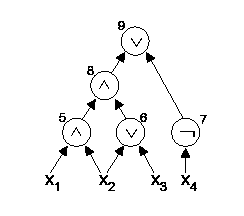
\includegraphics{img/bo/leprikl}
  \caption{Booleovský obvod $C_4$ z príkladu \ref{bo_prikl_le}} \label{bo_obr_lepriklad}
\end{figure}

\begin{definicia}
Postupnosť booleovských obvodov $\{ C_n\}$ veľkosti $S(n)$ a hĺbky
$D(n)$ je
\begin{enumerate}
  \item $\mathcal{U}_E$ - uniformná, ak existuje $DTS\; A$ taký,
  že $L(A)=L_e$ a slová $\langle n,g,p,y\rangle$ akceptuje v čase
  $\log S(n)$
  \item $\mathcal{U}_{E^*}$ - uniformná, ak existuje $ATS\; A$
  taký, že $L(A)=L_e$ a slová $\langle n,g,p,y\rangle$ akceptuje v
  čase $D(n)$ a priestore $\log S(n)$.
\end{enumerate}
\end{definicia}

Všimnime si, že priestor potrebný na akceptovanie jazyka $L_e$
nezávisí od dĺžky vstupného\linebreak slova, ale od nejakého
podslova vstupného slova. Preto nie je korektné na základe
definície $\mathcal{U}_E$ uniformity písať $L_e\in DTIME(\log
SIZE(C_n))$. Na vyjadrenie tejto situácie zavedieme špeciálne
označenie: $L_e\Subset DTIME(\log SIZE(C_n))$, a podobne pri
$\mathcal{U}_{E^*}$ uniformite:\newline $L_e\Subset
ATIMESPACE(DEPTH(n),log SIZE(C_n))$.

V ďalšom budeme predpokladať, že v jazyku $L_e$, ktorý prislúcha
postupnosti $BO$ $\{ C_n\}$, bude použité ``tesné'' (``bez dier'')
očíslovanie vrcholov t.j. ak má obvod $m$ vrcholov, tak čísla
vrcholov budú z množiny $\{1,\dots ,m\}$ resp. $\{ 0,\dots
,m-1\}$.

\begin{lema}
\label{bo_lema_uniformity}

Nech $\{ C_n\}$ je postupnosť $BO$, $L_e$ je jej príslušný
rozšírený jazyk prepojení, a nech $f(n)\in\Omega(\log SIZE(C_n))$.
Potom štandardný kód $\langle C_n\rangle$ sa dá vypočítať v
$DSPACE(f(n))$ práve vtedy, keď $L_e\Subset DSPACE(f(n))$.
\end{lema}

\begin{dokaz}
Dokážeme obe inklúzie:
\begin{description}
  \item[``$\Rightarrow$''] Máme $DTS\; A$ generujúci kód $\langle
  C_n\rangle$v priestore $f(n)$. Chceme zostrojiť $DTS\; A'$
  akceptujúci jazyk $L_e$ v rovnakom priestore. $A'$ bude na
  vstupnom slove $\langle n,g,p,y\rangle$ pracovať nasledovne:

  $A'$ najskôr overí, či v obvode $C_n$ existuje vrchol s čislom
  $g$. To urobí tak, že bude simulovať $A$ na vstupe $1^n$, až kým
  nevygeneruje slovo $\langle g,t,a,b$ v štandardom kóde. Ak
  $p=\varepsilon$, overí či $y=t$ (ak nie, tak slovo neakceptuje).
  Ak $p\in\{ L,R\}^+$, tak $A'$ potrebuje overiť, či
  $p$-predchodca vrchola $g$ má číslo $y$. To robí rekurzívne:
  \begin{itemize}
    \item ak $p=Lp'$, tak $A'$ simuluje $A$, až kým nevygeneruje
    $\langle a,t',a',b'\rangle$. Ak $p'=\varepsilon$, overí typ t.j.
    či $t'=y$ (ak nie, tak slovo neakceptuje). Inak opäť simuluje
    $A'$, až kým nevygeneruje $p'$-predchodcu vrchola $a$ atď.
    \item ak $p=Rp'$, tak $A'$ simuluje $A$, až kým
    nevygeneruje $\langle b,t',a',b'\rangle$, a pokračuje podobne
    ako v prvom prípade.
  \end{itemize}
  Na prácu $A'$ nám stačí priestor $f(n)$ (v zmysle $\Subset$ notácie),
  lebo v tomto priestore dokážeme simulovať $A$ a pamätať si jedno
  slovo štandardného kódu.
  \item[``$\Leftarrow$''] Máme $DTS\;A'$ akceptujúci jazyk $L_e$ v
  $\Subset$ priestore $f(n)$. Chceme zostrojiť generátor $A$. Na
  vstupnom slove $1^n$ potrebuje $A$ pre každý vrchol číslo $g$ v
  obvode $C_n$ zistiť jeho typ $t$ a jeho vstupy $a,b$, a potom
  zapísať na výstup štvoricu $\langle g,t,a,b\rangle$. To bude
  robiť nasledovne:

  $A$ bude postupne pre $g=0,1,2,\dots$ a $t=x,0,1,\wedge,\vee,I,\neg$
  simulovať $A'$ na vstupe $\langle n,g,\varepsilon,t\rangle$. Ak
  nejakú takúto štvoricu $A'$ akceptuje, znamená to, že v obvode
  $C_n$ sa nachádza vrchol s číslom $g$ a typom $t$. Na zistenie
  vstupov vrchola $g$ bude $A$ postupne pre $a=0,1,2,\dots$ simulovať
  $A'$ na vstupe $\langle n,g,L,a\rangle$. Ak $A'$ pre nejaké $a$
  akceptuje, zistili sme číslo vrchola, ktorý je ľavým vstupom
  vrchola $g$. Podobne, simulovaním $A'$ na vstupe $\langle
  n,g,R,b\rangle$ pre $b=0,1,2,\dots$, zistíme pravý vstup vrchola
  $g$. Teda $A$ môže na výstup zapísať $\langle g,t,a,b\rangle$.
  Toto bude $A$ vykonávať, až kým pre nejaké $g$ $A'$ neakceptuje
  ani jednu zo štvoríc $\langle n,g,\varepsilon,t\rangle$ pre
  všetky $t\in\{ x,0,1,\wedge,\vee,I,\neg\} $. To znamená, že vrchol s takýmto
  číslom v obvode $C_n$ nie je, a vďaka predpokladu o číslovaní
  vrcholov ``bez dier'' vieme, že $A$ už vygeneroval kódy všetkých
  vrcholov v obvode.

  Na túto prácu stačí $A$ priestor $f(n)$, lebo v tomto prietore
  dokáže simulovať $A'$ a pamätať si nejakú informáciu konštantnej
  dĺžky o práve generovanom vrchole.
\end{description}
\end{dokaz}

Teraz si ukážeme aké vzťahy sú medzi troma uniformitami
booleovských obvodov, ktoré sme doteraz spomenuli.

\begin{veta}
Medzi uniformitami platia nasledujúce vzťahy:
\begin{enumerate}
  \item $\mathcal{U}_E DEPTHSIZE(D(n),S(n))\subseteq\mathcal{U}_{BC}
  DEPTHSIZE(D(n),S(n))$
  \item $\mathcal{U}_E DEPTHSIZE(D(n),S(n))\subseteq\mathcal{U}_{E^*}
  DEPTHSIZE(D(n),S(n))$
  \item Nech $D(n)\geq\log^2 (S(n))$, potom\newline
  $\mathcal{U}_{BC} DEPTHSIZE(D(n),S(n))\subseteq\mathcal{U}_{E^*}
  DEPTHSIZE(D(n),S(n))$
\end{enumerate}
\end{veta}

\begin{dokaz}
Dokážeme všetky tri inklúzie:
\begin{enumerate}
  \item Nech $\{ C_n\}$ je $\mathcal{U}_E$-uniformná postupnosť
  $BO$. Z definície vieme, že príslušný jazyk prepojení $L_e\Subset
  DTIME(\log S(n))$. Zjavne žiadny $DTS$ nepoužije viac priestoru
  ako času, takže $L_e\Subset DSPACE(\log S(n))$. Potom z lemy
  \ref{bo_lema_uniformity} plynie, že štandardný kód $\{ C_n\}$ sa dá
  vypočítať v $DSPACE(\log S(n))$, teda $\{ C_n\}$ je
  $\mathcal{U}_{BC}$-uniformná.
  \item Nech $\{ C_n\}$ je opäť $\mathcal{U}_E$-uniformná, teda
  vieme, že $L_e\Subset DTIME(\log S(n))$. Zrejme\linebreak $L_e\Subset
  DTIMESPACE(\log S(n),\log S(n))$. Keďže $DTS$ je špeciálnym
  prípadom $ATS$, tak $L_e\Subset ATIMESPACE(\log S(n),\log
  S(n))$. Zrejme $D(n)\geq\log S(n)$, teda\newline $L_e\Subset
  DTIMESPACE(D(n),\log S(n))$, čo znamená, že $\{ C_n\}$ je
  $\mathcal{U}_{E^*}$-uniformná.
  \item Nech $\{ C_n\}$ je $\mathcal{U}_{BC}$-uniformná postupnosť booleovských obvodov,
  teda jej štandardný kód vieme vygenerovať v $DSPACE(\log S(n))$. Z
  lemy \ref{bo_lema_uniformity} vieme, že príslušný jazyk\linebreak prepojení $L_e\Subset
  DSPACE(\log S(n))$. Zo simulácie $DTS$ na $ATS$ (veta
  \ref{alter_veta_nspaceatime}) plynie\linebreak $L_e\Subset ATIMESPACE(\log^2 S(n),\log
  S(n))$. Z predpokladu $D(n)\geq\log^2 S(n)$ dostávame $L_e\Subset
  ATIMESPACE(D(n),\log S(n))$, čo znamená, že $\{ C_n\}$ je
  $\mathcal{U}_{E^*}$-uniformná.
\end{enumerate}
\end{dokaz}

\section{Porovnanie modelov $BO$ a $ATS$}

Prv než prejdeme k samotnému porovnaniu modelov, uvedieme si jeden
normálový tvar booleov\-ských obvodov, ktoré neobsahujú hradlo
negácie. Tento normálový tvar následne využijeme v ďalšej vete.

\begin{lema}
Pre každý $BO$ $C_n$ existuje ekvivalentný $BO$ $C'_n$ obsahujúci
len vrcholy typu $\wedge$, $\vee$, ``0'', ``1'', ``x'',
``$\overline{x}$'', kde ``$\overline{x}$'' označuje negáciu
vstupného vrchola ``x''.
\end{lema}

\begin{dokaz}
Majme daný $BO$ $C_n$. Chceme k nemu skonštruovať $BO$ $C'_n$,
ktorý nebude obsahovať hradlo $\neg$. Jediným miestom v obvode
$C'_n$, kde sa môže negácia prejaviť, je na vstupe nahradením
vstupného vrchola ``x'' jeho negáciou ``$\overline{x}$''.

Odstránenie hradiel $\neg$ z obvodu bude prebiehať nasledovne.
Obvod $C_n$ budeme prehľadávať (do šírky) od výstupného vrchola k
vstupným. Ak narazíme na hradlo $\neg$, budeme rozlišovať šesť
možných prípadov v závislosti na tom, aký vrchol je vstupom pre
nájdené hradlo:
\begin{description}
  \item[$\wedge$ :] Vstupom pre $\wedge$ sú nejaké hodnoty $A,B$.
  Vieme, že platí: $\neg(A\wedge B)=\neg A\vee\neg B$, teda
  vrcholy $\neg,\wedge$ nahradíme vrcholmi $\vee,\neg,\neg$ podľa
  obrázka \ref{bo_obr_nonnegbo}a.
  \item[$\vee$ :] Vstupom pre $\vee$ sú nejaké hodnoty $A,B$.
  Vieme, že platí: $\neg(A\vee B)=\neg A\wedge\neg B$, teda
  vrcholy $\neg,\vee$ nahradíme vrcholmi $\wedge,\neg,\neg$ podľa
  obrázka \ref{bo_obr_nonnegbo}b.
  \item[$\neg$ :] Vstupom pre $\neg$ je nejaká hodnota $A$. Platí $\neg(\neg
  A)=A$, teda vrcholy $\neg,\neg$ z obvodu vynecháme (obr. \ref{bo_obr_nonnegbo}c).
  \item[``0'' :] Vrcholy $\neg$,``0'' nahradíme vrcholom ``1''
  (obr. \ref{bo_obr_nonnegbo}d).
  \item[``1'' :] Vrcholy $\neg$,``1'' nahradíme vrcholom ``0''
  (obr. \ref{bo_obr_nonnegbo}e).
  \item[``x'' :] Vrchol $\neg$ a vstupný vrchol ``x'' nahradíme vstupným
  vrcholom ``$\overline{x}$'' s opačnou hodnotou (obr. \ref{bo_obr_nonnegbo}f).
\end{description}

\begin{figure}[!ht]
  \centering
  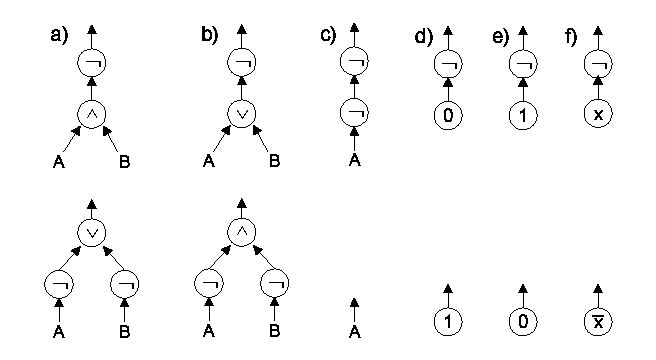
\includegraphics{img/bo/nonnegbo}
  \caption{Modifikácia $BO$ do normálového tvaru} \label{bo_obr_nonnegbo}
\end{figure}

V prvých dvoch prípadoch pri modifikácii obvodu opäť využívame
hradlá $\neg$. Treba si však uvedomiť, že tieto hradlá sú v obvode
o úroveň nižšie ako pôvodné nahradzované hradlo. Po príslušnej
úprave obvodu pokračujeme rekurzívne v prehľadávaní obvodu v
ďalšej úrovni až sa dostaneme k vstupným vrcholom.

Takto modifikovaný obvod $C'_n$ zrejme akceptuje rovnaký jazyk ako
$C_n$, lebo každá elementárna modifikácia bola logicky
ekvivalentná.
\end{dokaz}

\begin{veta}
Nech $S(n)\geq n$, potom platí:
\\ $\mathcal{U}_{E^*}DEPTHSIZE(D(n),S(n))\subseteq
ATIMESPACE(D(n),\log S(n))$.
\end{veta}

\begin{dokaz}
Nech $\{ C_n\}$ je $E^*$-uniformná postupnosť $BO$ hĺbky $D(n)$ a
veľkosti $S(n)$ v normálnom tvare z predchádzajúcej lemy, a nech
$A'$ je $ATS$ akceptujúci príslušný jazyk prepojení $L_e$ v čase
$D(n)$ a priestore $\log S(n)$. Chceme zostrojiť $ATS$ $A$
simulujúci $\{ C_n\}$. Uvažujme nejaké slovo $w=a_1\dots a_n\in
L(\{ C_n\})$ dĺžky $n$ (t.j. $w$ je akceptované $BO$ $C_n$).
Ukážeme, ako pracuje $A$ na vstupnom slove $w$.

$A$ uhádne číslo a typ výstupného vrchola $g_{out},t_{out}$. To
urobí tak, že sa existenčne rozvetví na veľa vetiev a v každej
vetve na pracovnú pásku zapíše binárne číslo dĺžky najviac $\log
S(n)$ a nejaký typ vrchola\footnote{Naozaj to bude tak, že pod
počiatočnou konfiguráciou sa rozvetví binárny strom hĺbky $\log
S(n)$, pričom pri prechode na nižšiu úroveň $A$ pripíše k už
vygenerovanému binárnemu číslu jeden bit podľa cesty v binárnom
strome od koreňa.}. Každá takáto vetva overí svoje hádanie t.j.
univerzálne spustí proces, v ktorom sa bude simulovať $A'$ na
vstupe\footnote{$A$ má v každej vetve na pracovnej páske zapísané
iba $\langle g_{out},t_{out}\rangle $, preto treba ešte vhodne
dopísať $\varepsilon$. $n$ na pracovnú pásku zapísať nemôžeme,
lebo jej priestor $\log S(n)$ je na to malý. Nie je však problém
upraviť $A'$ tak, aby $n$, keďže je kódované unárne, prečítal zo
vstupnej pásky $A$, kde ja zapísané vstupné slovo $w$ dĺžky $n$.}
$\langle n,g_{out},\varepsilon,t_{out}\rangle $, teda či vrchol s
číslom $g_{out}$ a typom $t_{out}$ v obvode $C_n$ existuje. Ak
taký vrchol existuje, potrebujeme overiť, či je naozaj výstupný,
teda opäť vo veľkom univerzálnom vetvení simuláciou $A'$
overujeme, či pre všetky $h\in\{ 0,1\}^*$ také, že $|h|\leq\log
S(n)$ platí $\langle n,h,L,g_{out}\rangle \not\in L_e$, a zároveň
$\langle n,h,R,g_{out}\rangle \not\in L_e$ to znamená, že vrchol
$g_{out}$ nemá nasledovníkov.

Uvažujme ďalej výpočet na vetve, ktorá úspešne uhádla výstupný
vrchol. Na pracovnej páske máme zapísané $\langle
g_{out},t_{out},\varepsilon\rangle $. V nasledujúcom bude $A$
hádať typy vrcholov, ktoré sú vstupmi $g_{out}$. $A$ sa podľa typu
$t_{out}$ ($\wedge$ univerzálne, $\vee$ existenčne) rozvetví
pričom v jednej vetve bude mať na páske zapísané $\langle
g_{out},L\rangle $ a v druhej $\langle g_{out},R\rangle $.

Vo všeobecnosti bude mať $A$ na páske zapísané $\langle g,p\rangle $,
kde $g$ je číslo nejakého vrchola a $p\in\{ L,R\}^*$ je nejaká
navigačná cesta dĺžky najviac $\log S(n)$. $A$ v tomto prípade
uhádne typ vrchola $g(p)$ ($p$-predchodca vrchola $g$) a univerzálne
sa rozvetví na dve vetvy:
\begin{itemize}
  \item V jednej overí, že hádal správne typ t.j. uhádne číslo
  $p$-predchodcu vrchola $g$ (teda v existenčnom vetvení si $A$
  zapíše na pásku binárne číslo $g(p)$) a overí, že hádal správne,
  teda simuluje $A'$ na vstupe $\langle n,g,p,g(p)\rangle $. Následne overí, že
  pre $p$-predchodcu vrchola $g$ hádal správny typ, teda simuluje
  $A'$ na vstupe $\langle n,g(p),\varepsilon,t_{g(p)}\rangle $.
  \item V druhej vetve pokračuje vo výpočte. To znamená, že podľa
  hádaného typu vrchola $g(p)$ sa ($\wedge$ univerzálne, $\vee$
  existenčne) rozvetví, pričom v jednej vetve si k navigačnej
  ceste $p$ na pásku pripíše $L$ a v druhej si pripíše $R$, teda
  $A$ bude v situácii kedy má na páske zapísané $\langle g,p'\rangle $, kde $p'$
  je v jednom prípade $pL$, v druhom $pR$. V oboch vetvách $A$
  postupuje rovnako ako sme naznačili vyššie.

  V prípade, že typ vrchola $g(p)$ je vstup, $A$ uhádne, ktorý
  i-ty vstup to je a či je typu ``$x_i$'' alebo
  ``$\overline{x}_i$''. Hádanie v univerzálnom vetvení overí, teda
  v jednej vetve simuluje $A'$ na vstupe
  $\langle n,g(p),\varepsilon,x_i\rangle $ resp.
  $\langle n,g(p),\varepsilon,\overline{x}_i\rangle $ a v druhej vetve výpočet
  končí s tým, že
  \begin{itemize}
    \item ak je vstup typu ``$x_i$'', tak $A$ akceptuje, ak $a_i=1$
    (neakceptuje, ak $a_i=0$)
    \item ak je vstup typu ``$\overline{x}_i$'', tak $A$
    akceptuje, ak $a_i=0$ (neakceptuje, ak $a_i=1$)
  \end{itemize}
\end{itemize}

Uvažujme teraz prípad, že dĺžka navigačnej cesty $p$ na páske
dosiahne hranicu $\log S(n)$. To je problém, pretože priestor
pracovnej pásky $A$ je ohraničený na $O(\log S(n))$ a naviac pri
väčšej dĺžke $p$ by sme už ani nemohli jednoducho overovať hádanie
simuláciou $A'$, lebo slová jazyka $L_e$ sú definované s
navigačnou cestou dĺžky najviac $\log S(n)$. V tomto prípade
postupojeme nasledovne:

$A$ má na páske zapísané $\langle g,p\rangle $, pričom $|p|=\log
S(n)$. V existenčnom vetvení uhádne číslo $h$ a typ $t_h$ vrchola
$g(p)$ a univerzálne
\begin{itemize}
  \item overí či $\langle n,g,p,h\rangle \in L_e$ a $\langle n,h,\varepsilon,t_h\rangle \in
  L_e$
  \item pokračuje vo výpočte, pričom na páske má zapísané
  $\langle h,t_h,\varepsilon\rangle $, teda sme v podobnej situácii, ako sme
  boli na začiatku po uhádnutí výstupného vrchola.
\end{itemize}

Z konštrukcie by malo byť vidieť, že skonštruovaný $ATS$ $A$
naozaj akceptuje práve slová z jazyka $L(\{ C_n\})$.

Zamyslime sa teraz nad časovou a priestorovou zložitosťou $A$:
\begin{itemize}
  \item Uhádnutie výstupného vrchola trvá čas $\log S(n)\leq D(n)$.
  \item Ak má $A$ na páske zapísanú cestu $p$ dĺžky menšej ako $\log
  S(n)$, tak $A$ sa v hlavnom výpočte (hádanie ďalšej úrovne
  $C_n$) posunie v konštantnom čase vďaka tomu, že pri
  rozvetvovaní stačí na páske predĺžiť cestu $p$ o $L$ resp. $R$.
  Všetky dlhé hádania a overovania sa robia v bočných vetvách
  výpočtu, a teda ich netreba do celkového času zarátať. Musíme si
  však uvedomiť, že tieto bočné vetvy sú dlhé najviac $D(n)$, lebo
  v nich $A$ buď háda, teda zapisuje na pásku (ale sú to vždy informácie
  dĺžky najviac $D(n)$), alebo simuluje $A'$, ten však z definície
  pracuje v čase $O(D(n))$.
  \item Každú $(\log S(n))$-tú úroveň výpočtu dosiahne dĺžka $p$
  hranicu $\log S(n)$. $A$ vtedy musí znova hádať v hlavnom
  výpočte číslo vrchola - na to spotrebuje čas $O(\log S(n))$.
  Keďže obvod má hĺbku $D(n)$, takýchto situácií sa počas výpočtu
  vyskytne $\frac{D(n)}{\log S(n)}$ krát. Na riešenie všetkých týchto
  situácií spotrebuje $A$ čas $O(\frac{D(n)}{\log S(n)} \log S(n))=O(D(n))$.
  \item Na koncoch jednotlivých vetiev výpočtu pri zisťovaní
  hodnoty i-teho vstupu musí $A$ presunúť hlavu nad tento symbol.
  Pri dĺžke vstupu $n$ by sme na túto operáciu potrebovali čas $O(n)$,
  čo je priveľa. Preto budeme uvažovať, že $ATS$ $A$ má rýchly
  prístup na vstupnú pásku, teda nám bude stačiť čas $\log n$, čo
  je menej ako $D(n)$ vďaka predpokladu $S(n)\leq n$ zo znenia
  vety.
  \item Počas celého výpočtu bolo na páske zapísané číslo nejakého
  vrchola dĺžky najviac $\log S(n)$, navigačná cesta dĺžky najviac
  $\log S(n)$ a typ vrchola konštantnej dĺžky, čo celkovo dáva
  nároky na priestor $O(\log S(n))$.
\end{itemize}
Z uvedeného vyplýva, že sme konštrukciou $ATS$ $A$ splnili
požiadavky na korektnosť akceptácie ako aj na časovú a priestorovú
zložitosť.
\end{dokaz}

\begin{veta}
Nech $S(n)\geq\log n$, potom pre vhodnú konštantu $k$ platí:\newline
$ATIMESPACE(T(n),S(n))\subseteq\mathcal{U}_E
DEPTHSIZE(T(n),k^{S(n)})$
\end{veta}

\begin{dokaz}
K danému $ATS\;A$ chceme zostrojiť postupnosť $BO$ $\{ C_n\}$
akceptujúcu jazyk $L(A)$. Skôr ako začneme konštruovať $\{ C_n\}$
zamyslime sa nad tým ako vyzerá výpočet na $ATS$.

Predstavme si úplný strom konfigurácií $ATS\;A$ na nejakom
vstupnom slove $w$. Na výpočet $A$ sa môžme pozerať aj ako na
vyhodnocovanie tohto stromu zdola. Každý vrchol reprezentujúci
akceptačnú konfiguráciu na konci nejakej vetvy v strome
konfigurácií ohodnotíme 1. Ostatné vrcholy na konci vetiev ako aj
nekonečné vetvy ohodnotíme 0. Každý vrchol reprezentujúci
univerzálnu konfiguráciu ohodnotíme 1 práve vtedy, keď všetci jeho
synovia majú hodnotu 1. Vrchol reprezentujúci existenčnú
konfiguráciu ohodnotíme 1 práve vtedy, keď aspoň jeden z jeho
synov má hodnotu 1. Vstupné slovo $w$ bude $A$ akceptovať práve
vtedy, keď koreň stromu (vrchol reprezentujúci počiatočnú
konfiguráciu $A$ na slove $w$) ohodnotíme 1.

Uvažujme teraz $ATS\;A$ v nasledovnom normálovom tvare:\newline
$A$ pracuje s binárnou vstupnou aj pracovnou abecedou, $A$ používa
rýchly prístup na vstupnú pásku (t.j. $A$ má špeciálnu pásku dĺžky
$\log n$, na ktorú keď v binárnom kódovaní zapíše číslo $j$,
dostane sa k $j$-temu symbolu na vstupe), úplný strom konfigurácií
je binárny a v každej vetve tohto stromu môže $A$ čítať vstup iba
raz, a to na konci (t.j. $A$ má špeciálne čítacie stavy $q^0$ a
$q^1$, do ktorých sa dostane na konci výpočtu vetvy, pričom v
stave $q^0$ očakáva na vstupe\footnote{na jednej pozícii vstupu
určenej číslom na špeciálnej páske} 0 (ak je na vstupe naozaj 0,
tak akceptuje, ak je tam 1, neakceptuje) a v $q^1$ očakáva na
vstupe 1).

Pozrime sa teraz na úplný strom konfigurácií $A$. Má $T(n)$
úrovní, pričom v nultej úrovni bude jediný vrchol reprezentujúci
počiatočnú konfiguráciu. Hľadaný $BO$ $C_n$ akceptujúci vstupné
slovo $w$ dĺžky $n$ bude vyzerať veľmi podobne. Každému vrcholu v
úplnom strome konfigurácií zodpovedá jeden vrchol v obvode $C_n$.

Vrcholu na úrovni $t$, ktorý reprezentuje
konfiguráciu\footnote{Uvažujeme tu konfiguráciu bez vstupu, lebo
každý FORKovaný výpočet používa len jeden symbol zo vstupu, takže
vstup v konfigurácii de facto nepotrebujeme. Na druhej strane
veľmi užitočná v konfigurácii je informácia o špeciálnej páske
určujúcej ktorý symbol sa má čítať na konci výpočtu.} $c$ v strome
konfigurácií zodpovedá v obvode $C_n$ vrchol s číslom $f(t,c)$,
kde $f:N\times N\rightarrow N$ je funkcia zachovávajúca tesné
očíslovanie vrcholov, pričom
\begin{itemize}
  \item ak $c$ je univerzálna konfigurácia, tak vrchol $f(t,c)$ je
  typu $\wedge$
  \item ak $c$ je existenčná konfigurácia, tak vrchol $f(t,c)$ je
  typu $\vee$
  \item ak $c$ je čítacia konfigurácia so stavom $q^0$ a na
  špeciálnej páske je zapísané číslo $j$, tak vrchol $f(t,c)$ je
  typu\footnote{Ak $A$ očakáva na vstupe 0 a naozaj tam 0 je, tak
  hradlo $\neg$ dostane na vstup 0 a na výstup pošle 1, čo signalizuje,
  že $A$ očakával správne. Naopak ak je na vstupe 1, tak hradlo $\neg$
  pošle na výstup 0, čo signalizuje, že $A$ sa mýlil. Analogicky to
  funguje pre stav $q^1$ a hradlo $I$.} $\neg$ a jeho vstupom je
  $j$-ty bit vstupného slova $w$
  \item ak $c$ je čítacia konfigurácia so stavom $q^1$ a na
  špeciálnej páske je zapísané číslo $j$, tak vrchol $f(t,c)$ je
  typu $I$ a jeho vstupom je $j$-ty bit vstupného slova $w$
  \item ak $c$ je akceptačná konfigurácia ale nie je čítacia, tak
  vrchol $f(t,c)$ je typu ``1''
  \item ak $c$ je odmietacia konfigurácia ale nie je čítacia, tak
  vrchol $f(t,c)$ je typu ``0''
\end{itemize}

\begin{figure}[!ht]
  \centering
  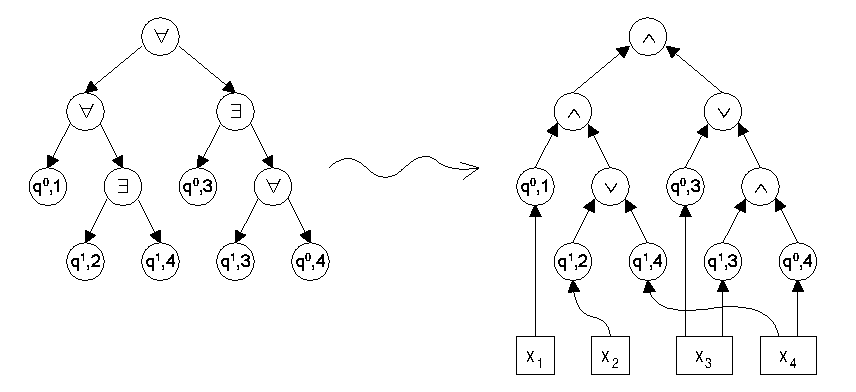
\includegraphics{img/bo/atsbo}
  \caption{Konštrukcia $BO$ k $ATS$} \label{bo_obr_atsbo}
\end{figure}

Vstupnými vrcholmi pre vrchol $f(t,c)$ sú vrcholy s číslami
$f(t+1,c_1)$ a $f(t+1,c_2)$ pričom platí $c\underset{A}{\vdash}
c_1$ a $c\underset{A}{\vdash} c_2$ (obr. \ref{bo_obr_atsbo}).

Takto zostrojený obvod $C_n$ pracuje presne tak ako výpočet $ATS$,
ktorý sme opísali na začiatku dôkazu. Teda príslušná postupnosť
$BO$ $\{ C_n\}$ zrejme akceptuje jazyk $L(A)$.

Pozrime sa ešte na miery zložitosti obvodu $C_n$. Obvod sme
zostrojili ``jedna k jednej'' vzhľadom na úplný strom konfigurácií
$ATS\;A$. Z toho plynie, že $DEPTH(C_n)=T(n)$. $SIZE(C_n)$
zodpovedá počtu vrcholov v strome konfigurácií. Keďže do
konfigurácií nezahŕňame vstup, tak počet všetkých možných
konfigurácií je $k^{S(n)}$ pre vhodné $k$. V zásade sa môže stať, že v úplnom
strome konfigurácií máme v dvoch rôznych vetvách vrcholy
reprezentujúce rovnakú konfiguráciu, čo by mohlo spôsobiť, že
počet vrcholov, a teda aj veľkosť $C_n$ by bola rádovo väčšia ako
$k^{S(n)}$. Ak ale uvažujeme výpočet $ATS$ ako FORKovanie
procesov, tak nie je potrebné, aby boli spustené dva rovnaké
procesy. Takže ak chce $ATS$ spustiť proces, ktorého kópia už
beží, tak tento duplicitný proces iba odkážeme na rovnaký už
bežiaci proces. To v booleovskom obvode znamená jedno prepojenie
medzi hradlami. Takže v konečnom dôsledku môžme uvažovať opäť
akýsi normálový tvar $ATS$, ktorý bude mať v úplnom strome
konfigurácií všetky konfigurácie disjunktné, a teda
$SIZE(C_n)=O(k^{S(n)})$.
\end{dokaz}

\chapter{Booleovské obvody ($BO$)}

\section{Definície a označenia}

\begin{definicia}
  Booleovký obvod je acyklický orientovaný graf,
  v ktorom vrcholy so vstupným stupňom 0 nazývame vstupné,
  vrcholy s výstupným stupňom 0 nazývame výstupné a vrcholom,
  ktoré nie sú vstupné, sú priradené $\wedge$, $\vee$, $\neg$ (AND, OR, NOT).
  Vstupné vrcholy označíme $x_1, x_2, ..., x_k$ alebo $0$ alebo $1$
\end{definicia}

Booleovský obvod počíta funkciu $f: B^n \rightarrow B^m$,
kde $n$ je počet vstupných a $m$ výstupných vrcholov.
Štandardne platí, že AND a OR má 2 vstupy a NOT jeden.
My budeme v nasledujúcom uvažovať, že booleovský obvod má len jeden výstup,
keďže obvod s $m$ výstupmi sa dá "rozbiť" na m obvodov,
ktoré majú len jeden výstup.\\
Je rozumné zamyslieť sa, kedy bude na výstupe booleovského obvodu
platný výsledok. Ak uvažujeme, že prechod vrcholom nám trvá
jednu časovú jednotku (po hrane je to zadarmo), po čase rovnom
najdlhšej ceste v grafe už určite bude na výstupe korektný výsledok.

\begin{definicia}
  Definujeme jazyky pomocou obvodov:\\
  Jazyk generovaný triedou obvodov
  $\{C_n\}_{n=0}^{\infty}$, kde $C_n$ má $n$ vstupných vrcholov označených\\
  $x_1,...,x_n$ a jeden výstupný vrchol,
  je $L(\{C_n\}_{n=0}^{\infty})=\{w \in \{0,1\}^* \mm $Obvod
  $C_{|w|}$ pri vstupe $a_1,...,a_{|w|}$, kde $w=a_1...a_{|w|}$, má hodnotu výstupu $1\}$
\end{definicia}

Booleovské obvody sú neuniformný model,
lebo pre každú dĺžku vstupu môže byť iný obvod.

\begin{definicia}
  Uniformné booleovské obvody sú také obvody $\{C_n\}_{n=0}^{\infty}$,
  pre ktoré existuje deterministický TS, ktorý na vstupe $1^n$
  (teda na vstupe obsahujúcom $n$ jednotiek)
  "vyrobí" obvod $C_n$
\end{definicia}

To nám zaručuje, že nemôžem vybehnúť mimo rekurzívne vyčísiteľné jazyky.

\section{Kódovanie Booleovských obvodov}

Booleovské obvody bodeme kódovať takto:
Jednotlivým vrcholom priradíme identifikátor - číslo.
Vrcholy $x_1,x_2,...,x_k$ budú mať identifikátory $1,2,...,k$.
Kód obvodu $C_n$ (označujeme $\langle C_n \rangle$) bude postupnosť štvoríc:
(číslo vrchola, funkcia, číslo ľavého vstupu, číslo pravého vstupu),
kde funkcia je z množiny $\set{\wedge, \vee, \neg, 0, 1, vstup}$\footnote{
  $0,1$ nám označujú booleovské konštanty}\\ Tu sa
dohodneme, že vrchol s číslom 0 označuje výstup.\\ O topologickom usporiadaní hovoríme
vtedy, keď vrchol sa objaví v kóde až vtedy, keď tam už boli jeho vstupy.

\section{Miery zložitosti pre booleovské obvody}

Pre booleovské obvody definujeme nasledujúce miery zložitosti:
\begin{itemize}
  \item{SIZE($C_n$) }označuje počet hradiel (okrem vstupných vrcholov) obvodu $C_n$
  \item{DEPTH($C_n$) }charakterizuje dĺžku najdlhšej cesty v obvode
\end{itemize}

\begin{priklad}
  Skalárny súčin dvoch booleovských vektorov vypočítame takto:\\ $(x_1, x_2, ..., x_n) .
  (y_1, y_2,..., y_n)=\underset{i=1}{\overset{n}\bigvee}(x_i\wedge y_i)$

  \begin{figure}[!ht]
    \centering
    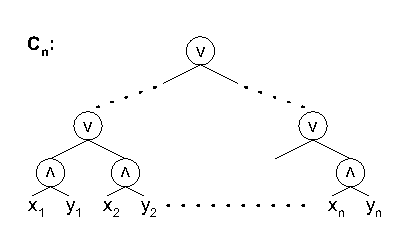
\includegraphics{img/bobr1}
    \caption{} \label{BObr1}
  \end{figure}

  \begin{itemize}
    \item DEPTH($C_n$)$=\log_2n$
    \item SIZE($C_n$)$=2n-1=O(n)$
  \end{itemize}

  Ukážme si, ako inak môžme skonštruovať obvod na výpočet skalárneho súčinu:

  \begin{figure}[!ht]
    \centering
    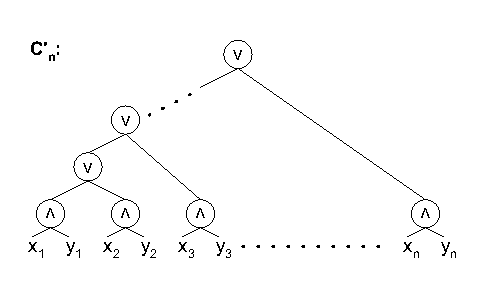
\includegraphics{img/bobr2}
    \caption{} \label{BObr2}
  \end{figure}

  \begin{itemize}
    \item DEPTH($C'_n$)$=O(n)$
    \item SIZE($C'_n$)$=O(n)$
  \end{itemize}

  Tu vidíme že aj napriek tomu, že sa nám zväčšila hĺbka, nedokázali sme zmenšiť počet
  hradiel.\\ Pre zaujímavosť: $|\langle C_n \rangle | =$SIZE($C_n$)$*\log$ SIZE($C_n$) lebo
  jedno hradlo dokážeme zapísať na priestor veľkosti $\log$ SIZE($C_n$) a počet hradiel je
  SIZE($C_n$)

\end{priklad}

\begin{priklad}
  Násobenie matíc: je to $n^2$ skalárnych súčinov,
  každý z nich sa robí nezávisle,
  teda podľa predchádzajúceho príkladu platí:
  \begin{itemize}
    \item DEPTH($C_n$)$=\log_2n$
    \item SIZE($C_n$)$=n^2*O(n)=O(n^3)$
  \end{itemize}
\end{priklad}

\begin{priklad}\label{Priklad1}
  Tranzitívny reflexívny uzáver booleovskej matice M:\\ 
  $M^*=I\vee M\vee M^2 \vee ...\vee M^n=(I\vee M)^n$,
  kde $M^i=\underbrace{M\wedge M\wedge ... \wedge M}_{i}$ \\
  Ideme len po $M^n$ preto, lebo ostatné sa už opakujú.

  \begin{figure}[!ht]
    \centering
    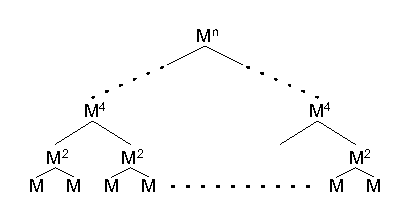
\includegraphics{img/bobr3}
    \caption{} \label{BObr3}
  \end{figure}

  Z obrázku \ref{BObr3} a predchádzajúceho príkladu vyplýva, že
  \begin{itemize}
    \item DEPTH($C_n$)$=O(\log^2n)$
    \item SIZE($C_n$)$=n*O(n^3)=O(n^4)$
  \end{itemize}

\end{priklad}

\section{Simulácie TS a BO}

\begin{veta}
  Ak $L$ je akceptovaný deterministickým 1-páskovým TS - A v čase T(n), potom $L$ sa dá
  definovať postupnosťou BO $\{C_n\}_{n=0}^{\infty}$ takých, že SIZE($C_n$)$=O(T^2(n))$
\end{veta}

\begin{dokaz}(Zatiaľ nekompletný) Zapíšeme konfigurácie TS pri výpočte na slove
  $a_1a_2...a_n$\\ do "tabuľky":
  \begin{center}
  \begin{tabular}{rcccccc}

     koncová konfigurácia:& $c_1$    &  $c_2$   & $...$ & $c_n$  & $...$ & $c_m$ \\

                          & $...$    &          &       &     \\

  konfigurácia po 1.kroku:& $b_1$    & $q_1a_2$ & $...$ & $a_n$     \\

  počiatočná konfigurácia:& $q_0a_1$ & $a_2$    & $...$ & $a_n$     \\

  \end{tabular}
  \end{center}
  kde počet stĺpcov tabuľky, ako aj počet riadkov je rovný T(n). $q_0a_1$, ako aj $q_1a_2$
  a ďalšie také, prehlásime za jeden symbol. Ak si očíslujeme riadky zdola hore číslami
  1,2,...,k a stĺpce zľava doprava číslami 1,2,...,l , tak obsah políčka (i,j) môžu
  ovplyvniť len políčka (i-1,j-1), (i-1,j) a (i-1,j+1) (Obrázok\ref{BObr4}) .
  \begin{figure}[!ht]
    \centering
    %\includegraphics{img/BObr4}
    \caption{CHÝBA OBRÁZOK} \label{BObr4}
  \end{figure}

  Políčko bude vyzerať takto:
    \begin{tabular}{|c|c|}
      \hline 1011 & 0101 \\
      \hline
    \end{tabular},
  kde v prvej časti je kód stavu (ak je tam 00...0 znamená to, že nie je tam
  stav) a v druhej časti je kód znaku.
\end{dokaz}

\begin{veta}
  Nech A je NTS so vstupnou páskou a jednou pracovnou páskou a vstupnou abecedou
  $\Sigma=\{0,1\}$. Ak A akceptuje slová dĺžky n v priestore $S(n)\geq \log\med n$, potom
  existuje booleovský obvod hĺbky $\approx S^2(n)$, ktorý akceptuje slová dĺžky n z $L(A)$
\end{veta}

\begin{dokaz}
  Keďže máme ohraničený priestor, tak vieme, že A môže byť v maximálne $k^{S(n)}$
  konfiguráciách pre nejakú konštantu $k$. Môžeme predpokladať, že A má jednoznačne
  danú\footnote{čiže jedinú jednu} akceptačnú konfiguráciu. Nech $\vdash$ je relácia na
  konfiguráciách. Keďže konfigurácii je $k^{S(n)}$, je $\vdash$ konečná relácia definovaná
  booleovskou maticou veľkosti $k^{S(n)}\times k^{S(n)}$.\\ Otázka, či $w\in L$, je otázka,
  či počiatočná konfigurácia na $w$ je v relácii $\overset{*}\vdash$ \footnote{tiež je
  konečná, tiež sa dá reprezentovať booleovskou maticou $k^{S(n)}\times k^{S(n)}$}s
  akceptačnou konfiguráciou.\\ Tranzitívny a reflexívny uzáver relácie $\vdash$ vieme podľa
  príkladu \ref{Priklad1} získať obvodom hĺbky $\log^2(k^{S(n)})$, čo je zhruba $S^2(n)$.
\end{dokaz}

\begin{definicia}
  Postupnosť booleovských obvodov $\{C_n\}_{n=0}^{\infty}$ je BC - uniformne
  konštruovateľná, ak existuje deterministický TS, ktorý pre každé n na vstupe $1^n$
  vypočíta kód obvodu $C_n$ v priestore $\log(SIZE(C_n))$
\end{definicia}

Ako vyzerá DTS:

\begin{figure}[!ht]
  \centering
  \includegraphics{img/bobr5}
  \caption{} \label{BObr5}
\end{figure}

\begin{description}
  \item $SIZE(C_n)$ - maximálny čas na pracovnej páske
  \item $SIZE(C_n).\log(SIZE(C_n))$ - veľkosť výstupu (a teda aj čas)
\end{description}

- o čase vieme povedať: $SIZE(C_n).\log(SIZE(C_n))$ - z obmedzenia DTS

\begin{oznacenie}
  $\mathcal{U}_{BC}SIZE \med DEPTH(S(n),D(n))$ je trieda jazykov, pre ktoré existuje
  postupnosť booleovských obvodov veľkosti $\approx S(n)$ a hĺbky $\approx D(n)$
\end{oznacenie}

\begin{veta}\label{Veta1}
  $L\in \mathcal{U}_{BC}Size(S(n))$ potom $L\in DTIME(Poly(S(n)))$
\end{veta}

\begin{dokaz}
  \begin{enumerate}
    \item Nech $A$ je DTS, ktorý vyrába obvod $C_n$ v prietore
      $\log(SIZE(C_n))$. Zostrojíme DTS $A'$,
      ktorý vyrobí na pracovnej páske kód $C_n$ simulovaním $A$ -
      to vieme v čase $[S(n)*\log(S(n))]$,
      čo je aj maximálna veľkosť pracovnej pásky
    \item Postupne priraďujeme hodnoty jednotlivým vrcholom $C_n$.
      Vstupným podľa vstupného slova, ostatným podľa hodnôt predchodcov.
      Keďže pre každý vrchol musím prebehnúť pásku a mám $S(n)$ vrcholov,
      teda výsledný čas DTS $A'$ bude približne $[S(n)*S(n)*\log(S(n))]$,
      čo je polynomiálna veľkosť.
  \end{enumerate}
\end{dokaz}

\begin{veta}
  \label{Veta2}
  $L\in \mathcal{U}_{BC}DEPTH(D(n))$ potom $L\in DSPACE(D(n))$
\end{veta}

\begin{dokaz}
  Zrejme $D(n)\geq \log(SIZE(C_n))$,
  lebo najviac hradiel v určitej hĺbke je v úplnom binárnom strome.
  Čiže v priestore $D(n)$ vieme simulovať konštruktor kódu obvodu $C_n$.
  Obvod budeme vyhodnocovať postorder prehľadávaním obvodu $C_n$.
  Pritom budeme opakovane generovať kódy jednotlivých vrcholov podľa toho,
  ktorý vrchol budeme práve potrebovať
  (lebo kód celého obvodu sa nám nevmestí do priestoru $D(n)$).
  Taktiež si musíme nejakým spôsobom pamätať,
  kde v strome sa nachádzame (navigáciu).
  Keby sme si navigáciu pamätali ako kódy všetkých vrcholov po ktorých sme šli,
  mohlo by to v najhoršom prípade zabrať veľmi veľa priestoru.
  Preto si budeme pamätať len navigačný reťazec(napríklad:0,0,1,...
  kde 0=vľavo a 1=vpravo).\\
  - z časového hľadiska je to veľmi neefektívna simulácia,
  keďže zakaždým od začiatku generujeme kódy vrcholov,
  ktoré momentálne potrebujeme, ale nepresiahneme priestor $D(n)$.
\end{dokaz}

\begin{dosledok}
  $PSPACE(\equiv DSPACE(Poly)=NSPACE(Poly))=\mathcal{U}_{BC}DEPTH(n^{O(1)})$
\end{dosledok}

\begin{definicia}
  Model počítača patrí do triedy počítačov druhej triedy, ak sekvenčný nedeterministický
  priestor je v polynomiálnom vzťahu s časom na danom modeli (jeden bol alternujúci stroj a
  druhý booleovský obvod)
\end{definicia}

Rýchlo paralelne počítateľné problémy - problémy, ktoré sa dajú počítať na nie príliš
hlbokých a nie príliš košatých obvodoch (polylogaritmická hĺbka a polynom. veľkosť).

\begin{definicia}
  (Nick's Class)
  \begin{description}
    \item $\mathcal{NC}^i = \mathcal{U}_{BC}SIZE \med DEPTH(n^{O(1)},\log^in)$
    \item $\mathcal{NC} = \underset{i\geq 1}\bigcup \mathcal{NC}^i$
  \end{description}
\end{definicia}

\begin{veta}
  $\mathcal{NC} \subseteq P $
\end{veta}

\begin{dokaz}
  Vyplýva z vety \ref{Veta1}
\end{dokaz}

Otvoreným problémom je rovnosť $\mathcal{NC}$ a $P$. Predpokladá sa ale, že podobne ako
pre $P$ a $NP$, aj tu platí: $\mathcal{NC}\neq P$

\begin{veta}
  $\mathcal{NC}^i \subseteq DSPACE(\log^in)$
\end{veta}

\begin{dokaz}
  Vyplýva z vety \ref{Veta2}
\end{dokaz}

\begin{dosledok}
  $\mathcal{NC} \neq PSPACE$
\end{dosledok}

\begin{poznamka}
  Vieme: $\mathcal{NC} \subseteq P \subseteq NP \subseteq PSPACE$, ale nevieme, kde je
  porušená súvislosť
\end{poznamka}

\begin{priklad}
  $L=\{ww^R\mm w\in \{0,1\}^* \} \in \mathcal{NC}^1$\\  Na obrázku \ref{BObr6} je
  znázornený obvod pre daný jazyk $L$. Ekvivalencia sa pomocou $\{\wedge,\vee,\neg\}$ dá
  napísať napríklad takto: $a\equiv b \Leftrightarrow (a\wedge b)\vee(\neg a \wedge \neg
  b)$.
\end{priklad}

\begin{figure}[!ht]
  \centering
  \includegraphics{img/bobr6}
  \caption{} \label{BObr6}
\end{figure}


Ak počítame funkcie, uvažujeme triedu funkcií $\mathcal{FNC}$\\ Násobenie matíc je v
$\mathcal{FNC}^1$ - hĺka je logaritmická, veľkosť polynomiálna. \\ Tranzitívny a
reflexívny uzáver je v $\mathcal{FNC}^2$ - hĺbka je $\log^2$. \\ - trieda $\mathcal{NC}$
(na rozdiel od $\mathcal{NC}^i)$ je dosť odolná voči uniformitám.

\section{Ďalšie druhy uniformity}

\begin{definicia}
  Majme danú postupnosť booleovských obvodov $\{C_n\}_{n=0}^\infty$. Jej príslušný
  rozšírený jazyk prepojení je nasledujúci jazyk: $L_e = \{\langle n,g,p,y\rangle \mm n,g
  \in \{0.1\}^*;\med p \in \{L,R\}^*;\\ |p|\leq \log(SIZE(C_n));\med y\in \{\times, \wedge,
  \vee, \neg\}\cup \{0,1\}^*$\footnote{$\times$ označuje vstupné hradlo}, pričom v obvode
  $C_n$ platí jedna z vecí:
  \begin{description}
    \item{(i) }$p=\varepsilon$ a hradlo číslo g je typu y
    \item{(ii) } $p\neq \varepsilon$ a hradlo $g(p)$ má číslo y $\}$
  \end{description}
  \begin{description}
    \item $g(L)$ je ľavý vstup hradla g
    \item $g(R)$ je pravý vstup hradla g
    \item $g(Lw)=(g(L))w$
    \item $g(Rw)=(g(R))w$
  \end{description}
\end{definicia}

\begin{priklad}
  Rozšírený jazyk prepojení, ktorého obvod $C_4$ je znázornený na Obr \ref{BObr7} vyzerá
  takto:\\
  $L_e=\{\underbrace{\med\med\med\med\med\med\med\med\med\med}_{C_1,C_2,C_3}\med,\overset{x_1}{\langle
  1111,1,\varepsilon,\times \rangle},\overset{x_2}{\langle 1111,10,\varepsilon,\times
  \rangle},\overset{x_3}{\langle 1111,11,\varepsilon,\times \rangle}, \overset{x_4}{\langle
  1111,100,\varepsilon, \times \rangle},\\ \overset{\mbox{\scriptsize 1.možnosť
  č.5}}{\langle 1111,101,\varepsilon, \wedge \rangle },\overset{\mbox{\scriptsize 2.možnosť
  č.5}}{\langle 1111,101,L, 1 \rangle },\overset{\mbox{\scriptsize 3.možnosť č.5}}{\langle
  1111,101,R, 10 \rangle },...,\overset{\mbox{\scriptsize 1.možnosť č.8}}{\langle
  1111,1000,\varepsilon, \vee \rangle }, \overset{\mbox{\scriptsize 2.možnosť č.8}}{\langle
  1111,1000,L, 111 \rangle },\\ \overset{\mbox{\scriptsize 3.možnosť č.8}}{\langle
  1111,1000,R, 100 \rangle },\overset{\mbox{\scriptsize 4.možnosť č.8}}{\langle
  1111,1000,LL, 101 \rangle },\overset{\mbox{\scriptsize 5.možnosť č.8}}{\langle
  1111,1000,LR, 110 \rangle },\overset{\mbox{\scriptsize 6.možnosť č.8}}{\langle
  1111,1000,LRL, 10 \rangle },...\}$

\end{priklad}

\begin{figure}[!ht]
  \centering
  \includegraphics{img/bobr7}
  \caption{} \label{BObr7}
\end{figure}

\begin{definicia}\label{Def1}
  Postupnosť booleovských obvodov $\{C_n\}_{n=o}^{\infty}$ veľkosti $S(n)$ a hĺbky $D(n)$
  je
  \begin{description}
    \item{(a) }$\mathcal{U}_E$ - uniformná, ak existuje DTS, ktorý akceptuje $L_e$ tak, že
    slová $\langle n,...\rangle$\footnote{ktoré popisujú n-ty obvod} akceptuje v čase
    $\log(S(n))$
    \item{(b) }$\mathcal{U}_{E^*}$ - uniformná, ak existuje ATS akceptujúci $L_e$ tak, že
    slová $\langle n,...\rangle$ akceptuje v čase $D(n)$ a priestore
    $\log(S(n))$\footnote{implicitne predpokladáme, že máme obvody očíslované, pričom
    nepoužívame veľmi veľké čísla}
  \end{description}
\end{definicia}

\begin{lema}\label{Lema1}
  Nech je daná postupnosť booleovských obvodov $\{C_n\}_{n=0}^{\infty}$ veľkosti $S(n)$.
  Nech $f(n)=\Omega (\log(S(n)))$. Potom $(1)$ štandardný kód obvodu $C_n$ sa dá vypočítať
  v $DSPACE(f(n)) \Leftrightarrow \med (2) \med L_e \widetilde{\in}$\footnote{priestor
  $f(n)$ na slovách $\langle n,...\rangle$}$DSPACE(f(n))$
\end{lema}

\begin{dokaz}
  \begin{description}
    \item{$(1)\Rightarrow (2)$ }Na zistenie, či $\langle n,g,p,y \rangle \in L_e$ budeme robiť
    nasledujúcu vec:
      \begin{description}
      \item{(i) }Budeme simulovať generátor kódu pre obvod $C_n$, kým nevyrobí $(g,t,a,b)$
      \item{(ii) }Overíme typ: ak $p=\varepsilon$: akceptuj ak $y=t$, inak $reject$
      \item{(iii) }Rekurzívne overíme číslo:
      \begin{description}
      \item ak $p=Lp'$:
      \begin{description}
      \item ak $p'=\varepsilon$ akceptuj ak $y=a$
      \item ak $p'\neq \varepsilon$ akceptuj ak $y=a(p')$\footnote{rekurzívne vytvorí
      $(a,.,.,.)$ a overuje}
      \end{description}
      \item ak $p=Rp'$:
      \begin{description}
      \item ak $p'=\varepsilon$ akceptuj ak $y=b$
      \item ak $p'\neq \varepsilon$ akceptuj ak $y=b(p')$
      \end{description}
      \end{description}
      \end{description}
  \item{$(2)\Rightarrow (1)$ }Štandardný kód pre obvod $C_n$ budeme generovať takto:
  \begin{description}
  \item{(i) }Zistíme najväčšie číslo hradla v obvode $C_n$\footnote{predpokladám
  číslovanie "bez dier"} \\ $g_{max}$ získam tak, že postupne testujem pre $g=0,1,2,...$ a
  $t\in \{\times, \wedge, \vee, \neg\}$, či $\langle n,g,\varepsilon, t\rangle \in L_e$,
  kým existuje také $t$
  \item{(ii) }Pre každé $g=0,1,...,g_{max}$ vyrobíme štvoricu $(g,t,g_L,g_R)$ tak, že $g_L$
  resp. $g_R$ nájdeme testovaním $\langle n,g,L,h \rangle \forall h \in
  \{0,1,...,g_{max}\}$ resp. $\langle n,g,R,h \rangle \forall h \in \{0,1,...,g_{max}\}$ a
  typ testujem tak, že testujem $\langle n,g,\varepsilon,t \rangle$ pre $t\in
  \{\times,\wedge,\vee,\neg \}$
  \end{description}
  \end{description}
\end{dokaz}

\section{Vzťahy uniformít}

\begin{veta}
  Platia nasledujúce vzťahy uniformít:
  \begin{enumerate}
    \item $\{C_n\}_{n=0}^{\infty}$ je $\mathcal{U}_E$ - uniformná $\Rightarrow$
      $\{C_n\}_{n=0}^{\infty}$ je $\mathcal{U}_{BC}$ - uniformná
    \item $\{C_n\}_{n=0}^{\infty}$ je $\mathcal{U}_E$ - uniformná $\Rightarrow$
      $\{C_n\}_{n=0}^{\infty}$ je $\mathcal{U}_{E^*}$ - uniformná
    \item Ak $D(n)\geq \log^2(S(n))$, potom \\ $\{C_n\}_{n=0}^{\infty}$ je
      $\mathcal{U}_{BC}$ - uniformná $\Rightarrow$ $\{C_n\}_{n=0}^{\infty}$ je
      $\mathcal{U}_{E^*}$ - uniformná
  \end{enumerate}
\end{veta}

\begin{dokaz}
  \begin{enumerate}
  \item Ak $\{C_n\}_{n=0}^{\infty}$ je $\mathcal{U}_E$ - uniformná
    $\overset{Def.\ref{Def1}}{\Longrightarrow} L_e \widetilde{\in} DTIME(\log(S(n)))
    \Rightarrow\\ L_e \widetilde{\in} DSPACE(\log(S(n)))
    \overset{Lema\ref{Lema1}}{\Longrightarrow}\{C_n\}_{n=0}^{\infty}$ je $\mathcal{U}_{BC}$ -
    uniformná
  \item $\{C_n\}_{n=0}^{\infty}$ je $\mathcal{U}_E$ - uniformná $\Rightarrow L_e
    \widetilde{\in} DTIME(\log(S(n))) \Rightarrow\\ L_e \widetilde{\in}
    DTIMESPACE(\log(S(n)),\log(S(n))) \Rightarrow\\ L_e \widetilde{\in}
    ATIMESPACE(\log(S(n)),\log(S(n))) \overset{D(n)\geq \log(S(n))}{\Longrightarrow}\\ L_e
    \widetilde{\in} ATIMESPACE(D(n),\log(S(n)))$ a to znamená, že $\{C_n\}_{n=0}^{\infty}$ je
    $\mathcal{U}_{E^*}$ - uniformná
  \item $\{C_n\}_{n=0}^{\infty}$ je $\mathcal{U}_{BC}$ - uniformná $\Rightarrow L_e
    \widetilde{\in} DSPACE(\log(S(n))) \Rightarrow\\ L_e \widetilde{\in}
    ATIMESPACE(\log^2(S(n)),\log(S(n))) \Rightarrow\\ L_e \widetilde{\in}
    ATIMESPACE(D(n),\log(S(n)))$, čiže $\mathcal{U}_{E^*}$ - uniformná
  \end{enumerate}
\end{dokaz}

\section{Booleovské obvody a alternujúce turingove stroje}

\begin{veta}\label{Veta3}
  $\mathcal{U}_{E^*} DEPTHSIZE(D(n),S(n))\subseteq ATIMESPACE(D(n),\log(S(n)))$,\\ kde
  $S(n)\geq n$\footnote{lebo inak by som do $S(n)$ nenapísal pointer na vstup}
  $(\Rightarrow D(n)\geq \log \med n)$
\end{veta}

\begin{dokaz}
  Budem predpokladať hradlá typu $\{\times, \bar{\times}, \wedge, \vee \}$\footnote{negáciu
  stlačím až na vstup}. ATS pre simuláciu $C_n$ bude pracovať takto:
  \begin{description}
    \item{(i) }Uhádne číslo výstupného vrchola $g_{OUT}$ (overí, že pre žiaden vrchol $h$
    neplatí $\langle n,h,L,g_{OUT} \rangle \in L_e$ ani $\langle n,h,R,g_{OUT} \rangle \in
    L_e$, lebo platí: ak som koreň, tak nie som syn)
    \item{(ii) }Vyhodnotí obvod tak, že postupne rozbehne procesy $CV(n,g,p)$\footnote{$p$ by
    mohlo mať veľkosť až $D(n)$, čo by sa nemuselo vojsť na $\log(S(n))$, keby sme to ďalej
    neošetrili}, ktoré akceptujú $\Leftrightarrow$ ak pre daný vstup hradlo $g(p)$ v $C_n$ je
    1.
    \\ Začne s $CV(n,g_{OUT},\varepsilon)$.\\ $CV(n,g,p)$ robí následovné: Kým platí
    $|p|<\log(S(n))$, ATS uhádne typ hradla $G(p)\med t\in
    \{\times,\bar{\times},\wedge,\vee\}$ a univerzálne
    \begin{enumerate}
    \item overí, či správne uhádol typ hradla tak, že uhádne číslo hradla
    $h\in\{0,1\}^{\log(S(n))}$ a univerzálne overí
    \begin{description}
    \item $\langle n,g,p,h\rangle\in L_e$
    \item $\langle n,h,\varepsilon,t \rangle \in L_e$
    \end{description}
    \item počíta ďalej
    \begin{description}
    \item ak $t=\wedge$ tak univerzálne
    \begin{description}
    \item $CV(n,g,pL)$
    \item $CV(n,g,pR)$
    \end{description}
    \item ak $t=\vee$ tak existenčne
    \begin{description}
    \item $CV(n,g,pL)$
    \item $CV(n,g,pR)$
    \end{description}
    \item ak $t=vstup$\footnote{$\times$ alebo $\bar{\times}$} tak uhádne, koľký v poradí
    vstup je to\footnote{číslo $i$ v binárnom zápise} a univerzálne
    \begin{description}
    \item overí, či to $i$ dobre hádal: $\langle n,g,p,"i"\rangle \in L_e$
    \item akceptuje
    \begin{description}
    \item ak $\times$ tak keď $a_i$\footnote{vstupné slovo je $a_1,a_2,...,a_n$} je 1
    \item ak $\bar{\times}$ tak keď $a_i$ je 0
    \end{description}
    \end{description}
    \end{description}
    \end{enumerate}
    Ak $|p|=\log(S(n))$\footnote{táto situácia nastane $\frac{D(n)}{\log(S(n))}$ krát}, stroj
    sa "posunie": uhádne číslo $h$ vrcholu $g(p)$\footnote{trvá to $\log(S(n))$} a
    univerzálne
    \begin{description}
    \item overí uhádnuté číslo $h$: $\langle n,g,p,h \rangle \in L_e$
    \item pokračuje $CV(n,h,\varepsilon)$
    \end{description}
    - v priemere čas na volanie "posunutia" stroja je konštantný\footnote{9 ľudí nakúpi za
    1Sk a 10. človek za 10Sk $\Rightarrow$ každý nakúpi za 2Sk}
  \end{description}
  Celkový čas: $\frac{D(n)}{\log(S(n))}.\log(S(n)) = D(n).c=D(n)$, kde c je konštanta.
\end{dokaz}

\begin{lema}
  K ľubovoľnému ATS A pracujúcemu v čase $T(n)$ a priestore $S(n)$ existuje ATS A'
  pracujúci v čase $T(n)$ a priestore $S(n)$ taký, že L(A)=L(A') a A' používa vstup v
  každej vetve najviac raz\footnote{každá vetva prečíta len jedno písmenko (bit) zo vstupu}
  a to na konci, pri prechode do $accept$ alebo $reject$ stavu\footnote{predpokladáme
  rýchly prístup k vstupným bitom}
\end{lema}

\begin{dokaz}
  Načrtneme si myšlienku dôkazu: tam, kde A čítal vstup, A' uhádne vstup a univerzálne sa
  rozvetví: v jednej vetve pokračuje v simulácii automatu A a v druhej overí uhádnutý vstup
  načítaním (ak sa rovnajú tak $accept$ inak $reject$).
\end{dokaz}

\begin{veta}\label{Veta4}
  $ATIMESPACE(T(n),S(n))\subseteq \mathcal{U}_E DEPTHSIZE(T(n),2^{O(S(n))})$, kde $T(n)\geq
  S(n) \geq \log\med n$
\end{veta}

\begin{dokaz}
  K danému ATS A zostrojíme postupnosť obvodov $\{C_n\}_{n=0}^{\infty}$ takto: Bez ujmy na
  všeobecnosti môžme predpokladať, že A sa vetví na max. 2 procesy v každej konfigurácii a
  každý proces číta najviac raz, a to na konci. Obvod $C_n$ zostrojíme z hradiel typu
  $\wedge,\vee,\neg, "0","1",id$\footnote{nerobí nič, len prepúšťa signál}. Hradlám bude
  prideľovať čísla tvaru $[t,c]$\footnote{uvažujeme zmysluplné číslovanie hradiel}, kde $t$
  je časový moment $0\leq t \leq \Gamma(n)$ veľkosti $\log(T(n))$ a $c$ je konfigurácia
  (bez informácie o vstupe) veľkosti $S(n)$\\ -takto budem mať očíslované vrcholy
  booleovského obvodu \\ -o čase môžme predpokladať, že bude $(const)^{S(n)}$\\Hradlu
  $[t,c]$ priradím typ
  \begin{description}
  \item {$\wedge$ } ak $c$ je univerzálna konfigurácia
  \item {$\vee$ } ak $c$ je existenčná konfigurácia
  \item {"0"} ak c je $reject$
  \item {"1"} ak $c$ je $accept$
  \end{description}
  Ak chce ísť čítať, prepne sa do stavu $q^0$, ak predpokladáme na vstupe 0 (ak načíta 0
  $\rightarrow \med accept$, ak 1 $\rightarrow \med reject$) a $q^1$, ak predpokladáme na
  vstupe 1 (ak načíta 1 $\rightarrow \med accept$, ak 0 $\rightarrow \med reject$).
  \begin{description}
  \item $\neg $ ak $c$ obsahuje čítací stav $q^0$
  \item $id $ ak $c$ obsahuje čítací stav $q^1$
  \end{description}
  Výstupný vrchol je $[0,$poč.konfig.$]$.\\ Nasledovníci:
  \begin{description}
  \item "obyčajný" vrchol $[t,c]$ má vstupné vrcholy $[t+1,c_1]$ a $[t+1,c_2]$ ak $c
  \underset{A}{\vdash}c_1$ a $c \underset{A}{\vdash}c_2$
  \item "čítací" vrchol $c$ má vstup vstupný vrchol $x_i$ ak $i$ je číslo v čítacom
  registri konfigurácii $c$.
  \end{description}
  Hĺbka obvodu zodpovedá $T(n)$, veľkosť $2^{O(S(n))}$. Ešte by sme mali ukázať, že obvod
  je $\mathcal{U}_E$ - uniformný:\\ $\langle n,g,p,y \rangle \in L_e$ len vtedy, keď
  $p=\varepsilon$ alebo $p$ "je nasledovník" - sledovanie cesty znamená robiť výpočet.
  Zmeny sú lokálne, je ich najviac $S(n)$\\ Ťažkosti, ktoré môžu nastať:\\ stroj by nemal
  akceptovať štvorice, kde $p$ je dlhšie ako $S(n)$ \\ ak by boli $T(n)$ a $S(n)$ rovné
  logaritmu, dostávam sa do problémov so vstupom.\\ Číslovanie je deravé, inak by to bol
  (možno aj) neriešiteľný problém.
\end{dokaz}

\begin{veta}
  $\mathcal{U}_{E^*}DEPTHSIZE(D(n),S(n))=ATIMESPACE(D(n),\log(S(n)))$
\end{veta}

\begin{dokaz}
  Priamy dôsledok vety \ref{Veta3} a vety \ref{Veta4}
\end{dokaz}

\begin{dosledok}
  $\mathcal{NC}=ATIMESPACE(\log^{O(1)}n,\log \med n)$
\end{dosledok}

\chapter{Parallel Random Access Machine $(PRAM)$}

Model, ktorý predstavujeme v tejto kapitole, je najviac podobný
reálnym paralelným architektúram. Ide o sústavu veľa (teoreticky
nekonečne) samostatných výpočtových jednotiek, ktoré nazývame
procesory. Každý procesor má svoju privátnu pamäť a sadu
inštrukcií podobných tým, ktoré poznáme z asembleru. Jednotlivé
procesory spolu komunikujú cez spoločnú zdielanú pamäť. Tento
model je akousi automatovou analogiou k modelu $PCGS$.
\\ Nebudeme sa zaoberať porovnávaním generatívnej sily $PRAMu$ s
modelmi Chomského\newline hierarchie, pretože už jeden samostatný
procesor $(RAM)$ má generatívnu silu Turingovho stroja. Zameriame
sa skôr na využitie sily tohto modelu na rýchle paralelné riešenie
problémov. V závere porovnáme model $PRAM$ s booleovskými obvodmi.

\section{Definície a označenia}

Skôr ako si zadefinujeme výpočtový model $PRAM$, s ktorým budeme
ďalej pracovať, povieme si niečo o jeho základnej základnej
výpočtovej jednotke, ktorou je $RAM$.

\subsection{$RAM$}

\begin{definicia}
$RAM$ (Random Access Machine) je výpočtový model pozostávajúci z
výpočtovej jednotky s pevne daným programom, jednej vstupnej a
jednej výstupnej pásky a neobmedzeného počtu registrov
$R_0,R_1,R_2,\dots$, pričom v jednom registri môže uchovávať
ľubovoľne veľké celé číslo (obr.\ref{pram_obr_modelram}). Program
výpočtovej jednotky je postupnosť jednoduchých\footnote{V sade
inštrukcií máme len jednoduché násobenie t.j. obsah registra krát
nejaká konštanta. Nemáme tu násobenie medzi registrami, lebo to by
dalo modelu $RAM$ príliš veľkú silu.} inštrukcií, ktoré sú uvedené
v tabuľke \ref{pram_tab_ram}. Výpočet začína prvou inštrukciou a
končí inštrukciou HALT.
\end{definicia}

\begin{figure}[!ht]
 \centering
 \includegraphics{img/pram/modelram.eps}
 \caption{Model $RAM$} \label{pram_obr_modelram}
\end{figure}

\begin{table}[!ht]\label{pram_tab_ram}
 \begin{center}
  \begin{tabular}{|c||c|}
   \hline
   inštrukcia & popis \\  \hline  \hline
   $READ$ & prečítaj nasledujúci symbol zo vstupu a zapíš ho do
   registra $R_0$ \\ \hline
   $WRITE$ & obsah registra $R_0$ zapíš na výstup \\ \hline
   $STORE\; R_i$ & obsah registra $R_0$ zapíš do registra $R_i$ \\
   \hline
   $COPY\; R_i$ & skopíruj obsah registra $R_i$ do registra $R_0$
   ($R_0\leftarrow [R_i]$) \\ \hline
   $CONST\; c$ & do registra $R_0$ zapíš hodnotu $c$ \\ \hline
   $ADD\; R_i$ & $R_0\leftarrow [R_0]+[R_i]$ \\ \hline
   $SUB\; R_i$ & $R_0\leftarrow [R_0]-[R_i]$ \\ \hline
   $MULT\; c$ & $R_0\leftarrow [R_0].c$ \\ \hline
   $DIV\; c$ & $R_0\leftarrow [R_0]/c$ \\ \hline
   $IFZERO\; i$ & ak register $R_0$ obsahuje 0, tak pokračuj
   inštrukciou $i$ \\ \hline
   $GOTO\; i$ & pokračuj inštrukciou $i$ \\ \hline
   $HALT accept$ & ukonči výpočet a akceptuj\\ \hline
   $HALT reject$ & ukonči výpočet a neakceptuj\\ \hline
  \end{tabular}
 \end{center}
\caption{Zoznam jednoduchých inštrukcií $RAMu$}
\end{table}

Model $RAM$ sa dá zadefinovať viacerými spôsobmi. Uvedenú
definíciu môžme, bez zmeny výpočtovej sily a zložitosti,
modifikovať tak, že vstup nebude zadaný na vstupnej páske, ale v
špeciálnych registroch, pričom v jednom z nich bude zadaná veľkosť
vstupu $n$ a v ďalšich $n$ registroch bude bit po bite zadaný
samotný vstup. \\ Ďalšou modifikáciou môže byť rovnakým spôsobom
upravený výstup, teda nie na výstupnej páske, ale opäť v (na to
určených) registroch.

\subsection{$PRAM$}

Prirodzeným rozšírením modelu $RAM$ v paralelných výpočtoch je
model $PRAM$, ktorý v sebe integruje viacero $RAMov$
komunikujúcich prostredníctvom zdieľanej pamäte.

\begin{figure}[!ht]
 \centering
 \includegraphics{img/pram/modepram.eps}
 \caption{Model $PRAM$} \label{pram_obr_modelpram}
\end{figure}

\begin{definicia}
$PRAM$ (Parallel Random Access Machine) je výpočtový model
pozostávajúci z neobmedzeného počtu $RAM$ procesorov označených
$P_0,P_1,P_2,\dots$ a neobmedzeného počtu spoločných (zdieľaných)
registrov $C_0,C_1,C_2,\dots$ Každý procesor $P_i$ má svoje
identifikačné číslo (index), má svoju vlastnú pamäť t.j.
ne\-ob\-me\-dze\-nú sadu registrov $R_{i,0},R_{i,1},R_{i,2},\dots$
a inštrukcie na priamy alebo nepriamy prí\-stup (read/write) do
spoločnej pamäte. Základná sada inštrukcii je zobrazená v tabuľke
\ref{pram_tab_pram}. Procesory sú zosynchronizované podľa globálnych
hodín, teda inštrukcie\linebreak v jednotlivých procesoroch sú
vykonávané v taktoch.
\\ Vstup $x\in\{ 0,1\}^n$ je zadaný nasledovne:
\begin{itemize}
  \item v registri $C_0$ je uložená dĺžka vstupu $n$
  \item v registri $C_i$ je uložený i-ty bit vstupu $x_i$
\end{itemize}
Výstup $y\in\{ 0,1\}^m$ je uložený v rovnakej forme.
\end{definicia}

\begin{table}[!ht]\label{pram_tab_pram}
 \begin{center}
  \begin{tabular}{|c||c|}
   \hline
   inštrukcia & popis \\  \hline  \hline
   $R_i\leftarrow [R_j]$ & skopíruj obsah registra $R_j$ do registra $R_i$
   \\ \hline
   $IDENT$ & do registra $R_0$ zapíš číslo procesora \\ \hline
   $CONST\; c$ & do registra $R_0$ zapíš hodnotu $c$ \\ \hline
   $ADD\; R_i$ & $R_0\leftarrow [R_0]+[R_i]$ \\ \hline
   $SUB\; R_i$ & $R_0\leftarrow [R_0]-[R_i]$ \\ \hline
   $MULT\; c$ & $R_0\leftarrow [R_0].c$ \\ \hline
   $DIV\; c$ & $R_0\leftarrow [R_0]/c$ \\ \hline
   $IFZERO\; i$ & ak register $R_0$ obsahuje 0, tak pokračuj
   inštrukciou $i$ \\ \hline
   $GOTO\; i$ & pokračuj inštrukciou $i$ \\ \hline
   $HALT$ & ukonči výpočet \\ \hline
  \end{tabular}
 \end{center}
\caption{Zoznam jednoduchých inštrukcií $PRAMu$}
\end{table}

\smallskip

Pri práve zadefinovanom modeli sa ukazujú dva závažné problémy:
\begin{enumerate}
  \item Nemôžeme predpokladať, že potenciálne nekonečne veľa
  procesorov sa bude podieľať na danom výpočte, a teda že budú
  všetky aktívne. Každý výpočet potrebuje isté množstvo
  procesorov, ktoré je závislé od vstupu resp. jeho dĺžky. Preto
  jeden z procesorov, označený ako $P_0$, má význačné postavenie,
  je to akýsi ``generál''. $P_0$ zapíše do špeciálneho registra $C_{-1}$
  maximálne číslo aktívneho procesora t.j. všetky procesory s
  menším indexom sú aktívne počas výpočtu. Teda najskôr je aktívny
  $P_0$ a ostatné čakajú, kým zapíše hodnotu maximálneho indexu
  procesora.\footnote{inou možnosťou riešenia tohoto problému by
  bolo zavedenie inštrukcie FORK, ktorou ľuboľný aktívny procesor môže
  aktivovať ďalšie, pričom na začiatku bude aktívny len procesor
  $P_0$}
  Výpočet skončí, keď skončí procesor $P_0$ t.j. vykoná HALT.
  \item Musíme vyriešiť konflikty pri viacnásobnom prístupe do
  spoločnej pamäte. Každá inštrukcia je vykonávaná v troch fázach.
  V prvej fáze je povolený prístup (ak treba) do spoločnej pamäte
  pre čítanie, potom sa vykoná príslušný výpočet pre danú
  inštrukciu, a nakoniec je povolený prístup (ak treba) do
  spoločnej pamäte pre zápis. Týmto sme oddelili prístup pre
  čítanie od prístupu pre zápis. Treba ešte vyriešiť situáciu, keď
  viac procesorov naraz pristupuje do spoločnej pamäte. Poznáme
  tri základné typy modelu $PRAM$:
  \begin{itemize}
    \item $CRCW-PRAM$ (Concurrent Read Concurrent Write) \\ Dovolíme
    procesorom súčasné čítanie aj súčasný zápis do spoločnej
    pamäte (registra). Tento typ má tri verzie:
    \begin{itemize}
      \item $PRIORITY:$ Ak chce do jedného registra zapisovať
      viacero procesorov, zápis vykoná len procesor s najmenším
      číslom z procesorov, ktoré žiadali o zápis.
      \item $COMMON:$ Ak chce do jedného registra zapisovať viacero
      procesorov, zápis sa uskutoční len vtedy, ak všetky
      procesory chcú zapísať rovnakú hodnotu.\newline V opačnom prípade sa
      výpočet zasekne.
      \item $ARBITRARY:$ Ľubovoľný\footnote{je to jediný
      nedeterministický prístup v modeli $PRAM$ t.j. môže sa stať,
      že pri opakovanom výpočte na rovnakom vstupe dostaneme
      rozdielne výstupy} z procesorov žiadajúcich o zápis zapíše
      svoju hodnotu do registra
    \end{itemize}
    \item $CREW-PRAM$ (Concurrent Read Exlusive Write) \\ Dovolíme\footnote{to
    znamená, že program (postupnosť inštrukcií) pre jednotlivé
    procesory musí spĺňať túto podmienku}
    procesorom súčasné čítanie spoločného registra, ale zapisovať do
    spoločného registra môže vždy len jeden procesor.
    \item $EREW-PRAM$ (Exlusive Read Exlusive Write) \\ Čítať a zapisovať do
    spoločného registra môže vždy len jeden procesor.
  \end{itemize}
\end{enumerate}

\section{Miery zložitosti}

Pri modeli $RAM$ uvažujeme tieto jenotkové miery zložitosti:
\begin{itemize}
  \item $TIME$ $T(n)$ = počet vykonaných inštrukcií
  \item $SPACE$ $S(n)$= počet použitých registrov
\end{itemize}
Z definície týchto mier je zrejmé, že neuvažujú veľkosť dát
(čísel), s ktorými inštrukcie pracujú, teda pracovať s veľkými
číslami je rovnako ``drahé'' ako pracovať s malými číslami. Z toho
plynie, že použitie jednotkovej miery nie je vhodné napr. pri
porovnávaní $RAM$ s Turingovým strojom. V takýchto prípadoch
uvažujeme tzv. logaritmickú mieru, ktorá zohľadňuje veľkosti čísel
pri jednotlivých operáciach. Logaritmická miera sa však používa
len zriedka, lebo v praxi máme aj tak obmedzenú veľkosť aj počet
registrov.

\pagebreak

Pri modeli $PRAM$ uvažujeme tieto jenotkové miery zložitosti:
\begin{itemize}
  \item $TIME$ $T(n)$ = počet krokov (taktov) procesora $P_0$ pri
  výpočte na vstupe dĺžky $n$
  \item $PROCESSORS$ $P(n)$ = maximálny počet aktívnych procesorov
  počas výpočtu na vstupe dĺžky $n$
\end{itemize}

Model $PRAM$ nemôže generovať príliš veľké (superpolynomiálne)
čísla. To znamená, že po $T(n)\leq \log n$ taktoch nebude ani v
jednom registri zapísané číslo s viac ako $O(T(n))$
bitmi.\linebreak Z toho plynie, že pri výpočte s časovou
zložitosťou $T(n)$ na $P(n)$ procesoroch $PRAM$ nespotrebuje na
uloženie dát viac ako $O(P(n).T^2(n))$ bitov. Máme teda adekvátnu
mieru pre pamäťové nároky $(SPACE)$.

\section{Výpočtová sila modelu $PRAM$}

Najskôr si ukážeme niekoľko príkladov výpočtov na modeli $PRAM$.

\begin{priklad}
Chceme vypočítať maximum z postupnosti $n$ zadaných čísel
$x_1,\dots ,x_n$ na\linebreak modeli $COMMON$ $CRCW-PRAM$.
\\ Vstup bude zadaný nasledovne: $C_0\leftarrow n$, $C_1\leftarrow
x_1,\dots ,C_n\leftarrow x_n$.
\\ Chceme\footnote{$[C]$ označuje obsah registra $C$, $C\leftarrow
a$ označuje zápis čísla $a$ do regitra $C$} výstup: $[C_0]=\max \{
x_1,\dots ,x_n\}$.
\\ Na výpočet použijeme $n^2$ procesorov ozn. $P_{i,j}$, kde
$i,j\in\{ 1,\dots ,n\}$ plus procesor $P_0$:
\begin{enumerate}
  \item Každý procesor $P_{i,1}$ vykoná: $C_{n+i}\leftarrow 0$
  \item Každý procesor $P_{i,j}$ vykoná\footnote{procesor nemá k dispozícii
  takú silnú inštrukciu, ale iste si vieme predstaviť jej simuláciu pomocou konečného
  počtu $PRAM$-inštrukcií}: $if\; [C_i]<[C_j]\; then\; C_{n+i}\leftarrow 1$
  \\ Uvedomme si, že tu nenastane žiadny konflikt pri súčasnom
  zápise viacerých procesorov do toho istého registra, pretože
  všetky procesory, ktoré budú chcieť zapísovať do registra
  $C_{n+i}$, budú chcieť zapísať 1.
  \item Každý procesor $P_{i,1}$ vykoná: $if\; [C_{n+i}]=0\;
  then\; C_0\leftarrow [C_i]$
  \\ Po kroku 2 je medzi registrami $C_{n+1},\dots ,C_{2n}$ jediný
  s nulovou hodnotou a platí
  \\ $[C_{n+i}]=0$ práve vtedy, keď $x_i=\max\{x_1,\dots ,x_n\}$
\end{enumerate}
Ako vidieť, vďaka použitiu polynomiálneho počtu procesorov, sa nám
podarilo nájsť maximum\linebreak z číselnej postupnosti v
konštantnom čase. Pri sekvenčných modeloch na to potrebujeme
lineárny čas.
\end{priklad}

\begin{priklad}
\label{pram_prikl_2}

Opäť chceme vypočítať maximum ako v predchádzajúcom príklade, ale
tentoraz na modeli $EREW-PRAM$.
\\ Vstup je zadaný tak isto ako v predchádzajúcom príklade.
Budeme\footnote{rovnakú myšlienku možno použiť pri úlohe sčítať
$n$ čísel} porovnávať dvojice registrov, pričom výsledky zapíšeme
do nových registrov, ktoré budeme opäť po dvojiciach porovnávať
atď. takže dostaneme binárny porovnávací strom
(obr.\ref{pram_obr_maxstrom}). Keďže používame stále nové a nové registre a
každý register má na starosti jeden procesor, tak procesory naraz
nečítajú ani nezapisujú do toho istého registra.

\begin{figure}[!ht]
 \centering
 \includegraphics{img/pram/maxstrom.eps}
 \caption{Výpočet maxima na $EREW-PRAM$} \label{pram_obr_maxstrom}
\end{figure}

Procesorovú zložitosť sme zmenšili $P(n)=n$, ale časová zložitosť
vzrástla $T(n)=\log n$.
\end{priklad}

\begin{priklad}
Ukážeme si, ako efektívne vieme triediť postupnosť čísel
$x_1,\dots ,x_n$ na modeli $CREW-PRAM$.
\\ Vo vstupných registroch $C_1,\dots ,C_n$ sú hodnoty $x_1,\dots
,x_n$. Chceme, aby po skončení výpočtu boli v registroch
$C_1,\dots ,C_n$ čísla zo vstupu v utriedenom poradí.
\\ Na výpočet použijeme $n^2$ procesorov ozn. $P_{i,j}$.
\begin{enumerate}
  \item Každý procesor $P_{i,j}$ vykoná: $if\; [C_i]<[C_j]\; then\;
  C_{i,j}\leftarrow 1\; else\; C_{i,j}\leftarrow 0$
  \item Každých $n$ procesorov $P_{i,1},\dots ,P_{i,n}$ sa bude
  podieľať na výpočte\footnote{sčítať $n$ čísel je podobný problém
  ako nájsť maximum z $n$ čísel (príklad \ref{pram_prikl_2})}:
  $C_{n+i}\leftarrow 1+$ $\sum\limits_{j=1}^{n} [C_{i,j}]$
  \item Každý procesor $P_{i,1}$ vykoná: $C_{C_{n+i}}\leftarrow [C_i]$
\end{enumerate}
Časová zložitosť $TIME$ je $T(n)=O(\log n)$, lebo prvý a tretí
krok výpočtu trvá konštantný čas a na druhý potrebujeme
logaritmický čas, počet procesorov je $P(n)=n^2$.
\\ Teraz ľahko vidíme, že problém triedenia je v $\mathcal{NC}$,
teda ho vieme efektívne paralelne riešiť.
\end{priklad}

\medskip
Jednotlivé modely $PRAM$ sú medzi sebou relatívne ekvivalentné,
takže je v zásade jedno, ktorý používame. Tento poznatok využijeme
pri porovnaní $PRAM$ s booleovskými obvodmi. Teraz si ukážeme
porovnanie medzi modelmi $EREW$ a $CRCW$.

\begin{veta}
$\mathcal{L}(EREW-PRAM)=\mathcal{L}(CRCW-PRAM)$
\end{veta}

\begin{dokaz}
Inklúziu $\subseteq$ netreba dokazovať, pretože z definícií
jednotlivých modelov vyplýva, že $EREW$ je špeciálnym prípadom
$CRCW$. Dokážeme opačnú inklúziu.
\\ Chceme simulovať $CRCW$ na $EREW$. Treba vyriešiť
situáciu, keď viacero procesorov chce naraz zapisovať do toho
istého registra t.j. treba z nich vybrať jeden, ktorý svoju
hodnotu do registra naozaj zapíše. Budeme z nich vyberať procesor
s najmenším číslom (takto vyriešime naraz všetky tri verzie modelu
$CRCW$).
\\ Pod každým registrom $C_i$ budeme mať binárny strom
pozostávajúci z nových registrov obsahujúcich čísla procesorov. V
listoch sú čísla všetkých aktívnych procesorov. Na začiatku každý
procesor pozná svoju pozíciu v tomto strome. Nie každý aktívny
procesor chce v danom okamihu zapisovať do $C_i$. Budeme postupne
po dvojiciach porovnávať obsahy registrov v tomto strome.
\\ Ak je procesor ľavý (t.j. s menším číslom) a chce zapisovať do $C_i$,
tak postúpi o úroveň vyššie (t.j. zapíše do príslušného registra
svoje číslo).
\\ Ak je procesor pravý, tak ``skúsi'', či jeho ľavý sused
postúpil.\footnote{To môžeme zabezpečiť tak, že každý postup o
úroveň vyššie bude prebiehať v troch krokoch. V prvom ľaví z
dvojice buď nechcú zapisovať a nepostupujú alebo postúpia, ak chcú
zapisovať, zatiaľ čo praví čakajú t.j. vykonajú inštrukciu NOP. V
druhom kroku praví, ak chcú zapisovať do $C_i$, tak čítajú obsah
registra zodpovedajúcemu vyššej úrovni. V treťom kroku praví, ak
zistili, že ľaví nezapísali svoje číslo do registra vyššej úrovne,
tak tam zapíšu svoje číslo.} Ak áno, tak v ďalšom už nechce
zapisovať do $C_i$, ak nie, tak postúpi o úroveň vyššie. Toto sa
vykonáva až ku koreňu stromu, teda ku koreňu sa dostane len jeden
procesor (s najmenším číslom z aktívnych procesorov, ktoré chceli
zapisovať do $C_i$) a ten zapíše svoju hodnotu do registra $C_i$.

Čítanie bude fungovať podobne, iba s tým rozdielom, že výpočet na
strome pod každým registrom sa bude vykonávať opačným smerom, aby
každý z procesorov, ktorý mal záujem čítať, sa dostal k $C_i$.

Keďže binárne stromy pod registrami majú výšku $\log P(n)$, tak
čítanie registra a zápis do registra sa z jedného kroku v modeli
$CRCW$ predĺži na $O(\log P(n))$ krokov v modeli $EREW$, a teda
čas $EREW$ modelu sa oproti $CRCW$ zhorší $O(\log P(n))$ násobne.
To je ale v celku dobrá simulácia.
\end{dokaz}

\section{Porovnanie modelov $BO$ a $PRAM$}

\begin{veta}
Nech $\{ C_n\}$ je $BC$-uniformná postupnosť booleovských obvodov
počítajúca funkciu $f_n:\{ 0,1\}^n\rightarrow\{ 0,1\}^m$ taká, že
$DEPTH(C_n)=(\log n)^{O(1)}$ a $SIZE(C_n)=n^{O(1)}$. Potom
existuje $CREW-PRAM$, ktorý počíta funkciu $f_n$ v čase
$T(n)=(\log n)^{O(1)}$ na $P(n)=n^{O(1)}$ procesoroch.
\end{veta}

\begin{dokaz}
Základná idea dôkazu spočíva v tom, že každé hradlo booleovského
obvodu $(BO)$ bude simulované jedným procesorom a každé spojenie
medzi hradlami (t.j. vstup resp. výstup)\linebreak v $BO$ bude
reprezentované jedným spoločným registrom. Potom každý procesor v
príslušnom takte, podľa hĺbky simulovaného hradla v $BO$, načíta
obsahy registrov prislúchajúce k vstupom simulovaného hradla,
vykoná daný výpočet podľa typu hradla, a následne zapíše výsledok
do registra prislúchajúceho k výstupu hradla (pozri obrázok
\ref{pram_obr_bopram3}, kde kružnice predstavujú procesory a obdĺžniky
registre). Tento register je zároveň vstupným registrom pre nejaký
iný procesor, ktorý simuluje ďalšie hradlo v $BO$.

\begin{figure}[!ht]
\centering
\includegraphics{img/pram/bopram3.eps}
\caption{Simulácia $BO$ na modeli $PRAM$} \label{pram_obr_bopram3}
\end{figure}

Každý procesor $P_i$, ktorý simuluje nejaké hradlo v $BO$, bude
mať v spoločnej pamäti vyhradené štyri registre $C_{i,IN1},
C_{i,IN2}, C_{i,OUT} ,C_{i,TYP}$, pričom v prvých dvoch budú
zapísané adresy dvoch vstupných registrov, do tretieho procesor
$P_i$ zapíše výstup a vo štvrtom bude zapísaný typ simulovaného
hradla. Procesor simulujúci vstupné hradlo samozrejme vystačí z
jedným registrom pre adresu vstupu.

Obsahy registrov $C_{i,IN1}, C_{i,IN2}, C_{i,TYP}$ závisia od
daného $BO$, a pred samotnou simuláciou ich podľa neho musíme
najskôr naplniť. Pripomeňme si, čo to znamená, že máme
daný\linebreak $BC$-uniformný booleovský obvod. Znamená to, že
poznáme $DTS\; A$ pracujúci s jednou\linebreak vstupnou, jednou
pracovnou a jednou výstupnou páskou, ktorý na vstupe $1^n$ zapíše
na výstupnú pásku kód $BO$ $C_n$, pričom pracovnú pásku má
obmedzenú na priestor $\log SIZE(C_n)$.

Chceme zostrojiť $PRAM$ simulujúci postupnosť $BO$ $\{ C_n\}$. To
znamená, že pre nejaký vstup dĺžky $n$ potrebujeme najskôr
odsimulovať výpočet $DTS\; A$, ktorý vygeneruje kód $BO$, potom ho
dekódovať (t.j. správne naplniť registre $C_{i,IN1}, C_{i,IN2},
C_{i,TYP}$), a nakoniec spustiť samotnú simuláciu výpočtu $BO$.

\pagebreak

\begin{itemize}
  \item Simulácia výpočtu $DTS\; A$:

  Čo vieme o $DTS\; A$? Ak uvažujeme, že $A$ pracuje na vstupe
  dĺžky $n$ v priestore\linebreak $S(n)=\log SIZE(C_n)$, tak počet všetkých
  možných konfigurácií $A$ je $k^{S(n)}.n.S(n)$ pre nejakú
  konštantu $k$, čo je rádovo $(SIZE(C_n))^{O(1)}$ čiže podľa
  predpokladu $n^{O(1)}$. Očíslujme si jednotlivé konfigurácie
  $1,2,\dots r$. Nech\footnote{takýto predpoklad môžeme urobiť,
  lebo pre daný vstup poznáme počiatočnú konfiguráciu a môžeme sa
  dohodnúť na jednej koncovej konfigurácií pre všetky výpočty, z
  ktorej sa už nedá dostať do inej konfigurácie} počiatočná
  konfigurácia má číslo $1$ a koncová má číslo $r$. Podľa
  predpokladu vety máme dostatok procesorov, aby sme každej
  konfigurácii priradili jeden procesor. Každému procesoru
  pridelíme dva registre zo spoločnej pamäte, jeden\footnote{POZOR:
  Nemýliť si s vyššie uvedeným rovnako nazvaným registrom,
  použitým pri samotnej simulácii $BO$} na výstup $(C_{j,OUT})$
  a druhý na číslo registra $(C_{j,REG})$.

  V prvom kroku každý procesor $P_j$ prislúchajúci j-tej
  konfigurácii odsimuluje jeden krok výpočtu $DTS\; A$ z tejto
  konfigurácie, pričom do prvého registra zapíše výstup
  zodpovedajúci tomuto kroku a do druhého zapíše číslo
  konfigurácie, do ktorej sa týmto krokom $A$
  dostal\footnote{tieto zápisy sú jednoznačné, keďže simulujeme
  deterministický stroj}. Keďže sme odsimulovali jeden krok $A$
  z každej konfigurácie, vyčerpali sme tým všetky možnosti
  $\delta$-funkcie, takže $\delta$-funkciu už simulovať
  nebudeme. V ďalšom chceme\linebreak jednotlivé kroky výpočtu $A$ vhodne
  ``pospájať'', aby spolu tvorili celý výpočet $A$, čím by sme
  dostali výsledný kód $\langle C_n\rangle$.

  V každom ďalšom kroku procesor $P_j$ vykoná:
  \begin{enumerate}
    \item  $C_{j,OUT}\leftarrow [C_{j,OUT}]\centerdot
    [C_{C_{j,REG},OUT}]$       , kde $\centerdot$ je
    zreťazenie\footnote{obsahmi registrov sú čísla v binárnom
    zápise, takže zreťazenie znamená nasledujúcu aritmetickú
    operáciu nad registrami: $C_{j,OUT}\leftarrow C_{j,OUT} +
    2^{|C_{C_{j,REG},OUT}|}.C_{C_{j,REG},OUT}$} obsahov registrov
    \item $C_{j,REG}\leftarrow [C_{C_{j,REG},REG}]$
  \end{enumerate}
  Každý procesor $P$ načíta registre procesora
  prislúchajúceho ku konfigurácii, ktorej číslo má procesor $P$ vo
  svojom druhom registri. Prvé (výstupné) registre zreťazí a toto
  zreťazenie zapíše ako novú hodnotu výstupného registra. Do
  druhého registra zapíše číslo konfi\-gurácie, ktoré načítal
  (obr.\ref{pram_obr_bopram1}). Každý procesor $P_j$ teraz reprezentuje dva
  kroky výpočtu $A$ začínajúci konfiguráciou číslo $j$. Po ďalšom
  kroku $PRAMu$ bude každý procesor $P_j$ reprezentovať štyri kroky
  výpočtu $A$ s výnimkou tých, ktoré už vo svojom druhom registri
  majú číslo koncovej konfigurácie, z ktorej sa už nedá dostať.
  Toto sa opakuje až kým procesor $P_1$ nemá vo svojom druhom
  registri hodnotu $r$. Vtedy sa simulácia generovania
  kódu\linebreak
  zastaví\footnote{realizáciu si môžeme predstaviť nasledovne:
  $P_1$ zapíše do nejakého špeciálneho booleovského registra, ktorý
  bol inicializovaný na TRUE, hodnnotu FALSE a program pre procesory
  upravíme tak, že dané inštrukcie budú vykonávať len vtedy, keď v
  tomto registri je hodnota TRUE} a $P_1$ bude mať vo svojom prvom
  registri celý výstup $A$, teda kód $BO$ $C_n$.
  Na obrázku \ref{pram_obr_bopram2} sú vyznačené procesory prislúchajúce ku
  konfiguráciám, v ktorých sa nachádza $DTS$ pri generovaní daného
  kódu. Hrubo vyznačené procesory sú pre nás významné z pohľadu
  generovania kódu. Tenko vyznačené procesory nám už nepomôžu k
  vygenerovaniu kódu, napriek tomu stále vykonávajú svoj program,
  pretože dopredu nevieme povedať, ktoré procesory budú významné a
  ktoré nie. Podobne nevieme dopredu určiť, ktoré procesory
  (konfigurácie) sa budú podielať na výpočte, a preto aj procesory,
  ktoré sa v konečnom dôsledku na výpočte podielať nebudú (na
  obrázku znázornené malými kružnicami v prvom riadku), vykonávajú
  svoj program.

\begin{figure}[!ht]
 \centering
 \includegraphics{img/pram/bopram1.eps}
 \caption{Jeden krok simulácie $DTS$} \label{pram_obr_bopram1}
\end{figure}

\begin{figure}[!ht]
 \centering
 \includegraphics{img/pram/bopram2.eps}
 \caption{Generovanie kódu $BO$ na modeli $PRAM$} \label{pram_obr_bopram2}
\end{figure}

  Keďže po každom kroku $PRAMu$ sa dĺžka odsimulovaného výpočtu $A$
  zdvojnásobí, tak na odsimulovanie celého výpočtu vystačíme s
  časom logaritmus z počtu konfigurácií, čo je $O(\log
  SIZE(C_n))$.

  \item Dekódovanie:

  Predpokladajme, že už máme v nejakom registri kód $\langle C_n\rangle$. Ten
  je v tvare:

   \centerline{
  ($\langle$ číslo hradla,typ hradla,číslo ľavého vstupu, číslo
  pravého vstupu $\rangle$)$^*$}
  Zrejme dĺžka kódu je $|\langle C_n\rangle |=O(SIZE(C_n).
  \log SIZE(C_n))$. Opäť máme dostatok procesorov, aby sme nimi
  ``pokryli'' každý symbol výstupu. Každý procesor $P_j$ načíta
  register s kódom $\langle C_n\rangle$ a akoby nastaví svoju čítaciu
  hlavu na j-ty symbol kódu $\langle C_n\rangle$. Procesory samozrejme žiadne
  čítacie hlavy nemajú, ale ľahko si vieme predstaviť, že $PRAM$ by
  vedel na jeden krok ``rozložiť'' obsah registra na veľa registrov
  obsahujúcich po jednom symbole, a potom by už procesory pracovali
  nad registrami ako je to v modeli $PRAM$ zvykom a nie s čítacou
  hlavou ako prezentujeme tu.

  Po prvom kroku prestanú pracovať všetky procesory, ktoré
  neprečítali na vstupe symbol\footnote{všetky symboly sú zakódované
  binárne, takže procesory prestanú pracovať po tom ako rozpoznajú
  symbol ``(''} ``(''. Tie, ktoré ``('' prečítali
  (t.j. boli nastavené na začiatok podslova v kóde $\langle C_n\rangle$
  reprezentujúce kód nejakého hradla), v každom ďalšom kroku
  prečítajú jeden symbol, až kým neprečítajú ``)'' (t.j. koniec
  kódu hradla). Každý takýto procesor ``zistí'' informácie o
  jednom hradle $BO$, teda číslo hradla, typ hradla a čísla
  vstupov, a zapíše ich do príslušných registrov $C_{i,IN1},
  C_{i,IN2}, C_{i,TYP}$.

  Keďže čísla hradiel sú v kóde zapísané v binárnom tvare, tak
  dĺžka kódu jedného\linebreak hradla je $O(\log SIZE(C_n))$. Každý procesor
  potrebuje prečítať kód jedného hradla a\linebreak zapísať získané
  informácie do registrov. Preto čas, ktorý na dekódovanie
  potrebujeme, je $O(\log SIZE(C_n))$.

  \item Simulácia výpočtu $BO$:

  Teraz už máme všetko pripravené na simuláciu výpočtu $BO$, teda
  v registroch  $C_{i,IN1}$, $C_{i,IN2}$, $C_{i,TYP}$ sú zapísané
  správne hodnoty prislúchajúce simulovanému $BO$. Predpo\-kladajme,
  že všetky registre $C_{i,OUT}$ sú inicializované na nejakú
  NILovú hodnotu\footnote{vzhľadom na to, že vo výstupných
  registroch budú len hodnoty 0 alebo 1, hodnotu NIL môže
  reprezentovať akákoľvek iná hodnota}. Procesor $P_i$ bude
  vykonávať program:
  \begin{enumerate}
    \item načítaj obsahy registrov $C_{i,IN1}, C_{i,IN2}, C_{i,TYP}$
    \item čakaj kým platí: $[C_{C_{i,IN1}}] = NIL$ a $[C_{C_{i,IN2}}] = NIL$
    \item vykonaj operáciu podľa typu hradla $[C_{i,TYP}]$ so
    vstupmi $[C_{C_{i,IN1}}], [C_{C_{i,IN2}}]$
    \item zapíš výsledok operácie do registra $C_{i,OUT}$
  \end{enumerate}
  Na vykonanie tohto programu potrebuje každý procesor čas najviac
  $(\log n)^{O(1)}$, pretože na druhom riadku bude procesor čakať
  toľko krokov koľko je hĺbka hradla v $BO$ a z predpokladu vieme, že
  $DEPTH(C_n)=(\log n)^{O(1)}$, ostatné riadky programu sa
  vykonajú v konštantnom čase.
\end{itemize}

Z dôkazu ľahko vidieť, že sme splnili požiadavky kladené na časovú
a procesorovú zložitosť, ako aj na model $CREW-PRAM$.
\end{dokaz}

\begin{veta}
Nech $M$ je $CREW-PRAM$, ktorý v čase $T(n)={(\log n)}^{O(1)}$ a s
počtom procesorov $P(n)=n^{O(1)}$ počíta funkciu $f$. Potom
existuje konštanta $k$ a $BC$-uniformná postupnosť booleovských
obvodov $\{ C_n\}$ taká, že $C_n$ počíta na vstupe $x_1\dots x_n$
výstup $y_{11}y_{12}\dots y_{ij}\dots$ kde $y_{ij}$ je hodnota
j-teho bitu spoločného registra $C_i$ v čase $T(n)$ pre $1\leq
i\leq P(n).T(n)$ a $1\leq j\leq k.T(n)$, pričom $DEPTH(C_n)={(\log
n)}^{O(1)}$ a $SIZE(C_n)=n^{O(1)}$.
\end{veta}

\begin{dokaz}
Chceme zostrojiť $BO$ simulujúci $CREW-PRAM$. Vstupom pre $M$ je
prvých $n$ spoločných registrov $C_1,\dots ,C_n$. Vstupom
$x_1\dots x_n$ pre $BO$ $C_n$ sú obsahy týchto registrov\linebreak
v čase $T_0$.

Výpočet $M$ závisí od postupnosti inštrukcií jenotlivých
procesorov. Pre každú inštrukciu zostrojíme elementárny obvod
simulujúci túto inštrukciu. Vstupom preň bude obsah
registra\linebreak (registrov), s ktorým príslušná inštrukcia
pracuje a výstupom bude nový obsah výstupného registra. Uvedomme
si, že za nášho predpokladu existencie konštanty $k$ takej, že
$1\leq j\leq k.T(n)$ (t.j. vieme ohraničiť maximálnu veľkosť
registra počas celého výpočtu), každú inštrukciu vieme simulovať
elementárnym obvodom obsahujúcim konečný počet hradiel.

\begin{figure}[!ht]
 \centering
 \includegraphics{img/pram/prambo.eps}
 \caption{Simulácia výpočtu $PRAM$ na $BO$} \label{pram_obr_prambo}
\end{figure}

$C_n$ bude mať $T(n)$ úrovní, pričom v i-tej úrovni budeme mať
obsahy všetkých registrov (bit po bite) v čase $T_i$. Dosiahneme
to tak, že medzi (i-1). úroveň a i-tu úroveň umiestnime (a vhodne
pospájame) elementárne obvody prislúchajúce k i-tym inštrukciám
všetkých aktívnych procesorov (obr.\ref{pram_obr_prambo}). Takže na
poslednej úrovni budú obsahy registrov v čase $T(n)$, čo zodpovedá
výstupu $M$.

Vďaka predpokladom o počte $(1\leq i\leq P(n).T(n))$, veľkosti
$(1\leq j\leq k.T(n))$ registrov a z toho vyplývajúcej konečnej
veľkosti elementárnych obvodov dostávame zložitosti pre $C_n$:
$DEPTH(C_n)={(\log n)}^{O(1)}$ a $SIZE(C_n)=n^{O(1)}$.

Teda dokázali sme ekvivalentnosť mier zložitosti medzi týmito
dvoma modelmi t.j. čas na modeli $PRAM$ zodpovedá hĺbke na $BO$ a
počet procesorov na $PRAM$ zodpovedá veľkosti $BO$.
\end{dokaz}

\begin{dosledok}
Model $PRAM$ je v druhej počítačovej triede.
\end{dosledok}

\begin{dosledok}
Triedu $\mathcal{NC}$ môžeme pomocou modelu $PRAM$ zadefinovať
nasledovne: \\ \centerline{$\mathcal{NC}=TIMEPROCESSORS((\log
n)^{O(1)},n^{O(1)})$}
\end{dosledok}


\bibliographystyle{alpha}
\bibliography{literatura}

\end{document}
